\newlength{\descwidth}
\setlength{\descwidth}{2in}
\newpage
\begin{center}{\Large\verb|ALPH|}\end{center}
\subsection{ALPH---An alpha magnet implemented as a matrix, up to 3rd order.}
An alpha magnet implemented as a matrix, up to 3rd order.
\\
Parallel capable? : yes\\
GPU capable? : yes\\
Back-tracking capable? : no\\
\begin{tabular}{|l|l|l|l|p{\descwidth}|} \hline
Parameter Name & Units & Type & Default & Description \\ \hline 
XMAX & $M$ & double &  0.0 & size of alpha  \\ \hline 
XS1 & $M$ & double &  0.0 & inner scraper position relative to XMAX  \\ \hline 
XS2 & $M$ & double &  0.0 & outer scraper position relative to XMAX  \\ \hline 
DP1 &  & double &   -1 & inner scraper fractional momentum deviation  \\ \hline 
DP2 &  & double &   1 & outer scraper fractional momentum deviation  \\ \hline 
XPUCK & $M$ & double &   -1 & position of scraper puck  \\ \hline 
WIDTHPUCK & $M$ & double &  0.0 & size of scraper puck  \\ \hline 
DX & $M$ & double &  0.0 & misalignment  \\ \hline 
DY & $M$ & double &  0.0 & misalignment  \\ \hline 
DZ & $M$ & double &  0.0 & misalignment  \\ \hline 
TILT &  & double &  0.0 & rotation about incoming longitudinal axis  \\ \hline 
PART &  & short &  \verb|0| & 0=full, 1=first half, 2=second half  \\ \hline 
ORDER &  & short &  \verb|0| & matrix order [1,3]  \\ \hline 
GROUP &  & string & NULL & Optionally used to assign an element to a group, with a user-defined name.  Group names will appear in the parameter output file in the column ElementGroup  \\ \hline 
\end{tabular}

\vspace*{0.5in}
\input{alph.tex}
\newpage
\begin{center}{\Large\verb|APCONTOUR|}\end{center}
\subsection{APCONTOUR---An aperture (or its inverse) defined by (x, y) points in an SDDS file.}
An aperture (or its inverse) defined by (x, y) points in an SDDS file.
\\
Parallel capable? : yes\\
GPU capable? : no\\
Back-tracking capable? : no\\
\begin{tabular}{|l|l|l|l|p{\descwidth}|} \hline
Parameter Name & Units & Type & Default & Description \\ \hline 
L & $M$ & double &  0.0 & length  \\ \hline 
TILT & $RAD$ & double &  0.0 & rotation about longitudinal axis  \\ \hline 
DX & $M$ & double &  0.0 & misalignment  \\ \hline 
DY & $M$ & double &  0.0 & misalignment  \\ \hline 
DZ & $M$ & double &  0.0 & misalignment  \\ \hline 
RESOLUTION & $M$ & double &  0.0 & z resolution of finding intersection  \\ \hline 
INVERT &  & short &  \verb|0| & if non-zero, contour defines an obstruction rather than an aperture  \\ \hline 
STICKY &  & short &  \verb|0| & if non-zero, effect persists in downstream elements until canceled or replaced  \\ \hline 
CANCEL &  & short &  \verb|0| & if non-zero, sole effect is to cancel previous sticky APCONTOUR  \\ \hline 
FILENAME &  & STRING &   NULL            & name of file containing contour data  \\ \hline 
XCOLUMN &  & STRING &   NULL            & name of column containing x data  \\ \hline 
YCOLUMN &  & STRING &   NULL            & name of containing y data  \\ \hline 
GROUP &  & string & NULL & Optionally used to assign an element to a group, with a user-defined name.  Group names will appear in the parameter output file in the column ElementGroup  \\ \hline 
\end{tabular}

\vspace*{0.5in}
The \verb|STICKY| parameter results in the aperture contour being applied inside subsequent \verb|CCBEND|,
\verb|CSBEND|, \verb|CSRCSBEND|, \verb|KQUAD|, \verb|KSEXT|, \verb|KOCT|, and \verb|KQUSE| elements, as well as at the
end of other downstream elements. This continues until another \verb|APCONTOUR| element asserts a new contour, or uses
\verb|CANCEL=1| to cancel the feature.

\newpage
\begin{center}{\Large\verb|BGGEXP|}\end{center}
\subsection{BGGEXP---A magnetic field element using generalized gradient expansion.}
A magnetic field element using generalized gradient expansion.
\\
Parallel capable? : yes\\
GPU capable? : no\\
Back-tracking capable? : no\\
\begin{tabular}{|l|l|l|l|p{\descwidth}|} \hline
Parameter Name & Units & Type & Default & Description \\ \hline 
L & $M$ & double &  0.0 & insertion length  \\ \hline 
LFIELD & $M$ & double &   -1 & expected length of the field map. If negative, use L.  \\ \hline 
FILENAME & $NULL$ & STRING &   NULL            & name of file generalized gradient data  \\ \hline 
STRENGTH & $NULL$ & double &   1 & factor by which to multiply field  \\ \hline 
TILT & $RAD$ & double &  0.0 & rotation about longitudinal axis  \\ \hline 
DX & $M$ & double &  0.0 & misalignment  \\ \hline 
DY & $M$ & double &  0.0 & misalignment  \\ \hline 
DZ & $M$ & double &  0.0 & misalignment  \\ \hline 
BX & $T$ & double &  0.0 & add BX*STRENGTH to Bx field  \\ \hline 
BY & $T$ & double &  0.0 & add BY*STRENGTH to By field  \\ \hline 
MAXIMUM\_M &  & short &   -1              & data with m greater than this is ignored  \\ \hline 
MAXIMUM\_2N &  & short &   -1              & data with 2*n greater than this is ignored  \\ \hline 
Z\_INTERVAL &  & short &   1               & input z data is sampled at this interval  \\ \hline 
SYMPLECTIC &  & short &  \verb|0| & if nonzero, use implicit symplectic integrator. At minimum, should always be used to validate the sufficiency of the non-symplectic integrator.  \\ \hline 
SYNCH\_RAD &  & short &  \verb|0| & if nonzero, include classical, single-particle synchrotron radiation  \\ \hline 
ISR &  & short &  \verb|0| & if nonzero, include incoherent synchrotron radiation (quantum excitation)  \\ \hline 
PARTICLE\_OUTPUT\_FILE &  & STRING &   NULL            & name of file for phase-space and field output. Use for debugging only!  \\ \hline 
IS\_BEND &  & short &  \verb|0| & if nonzero, magnet is a bending magnet; vertex, entry, and exit points should be defined.  \\ \hline 
\end{tabular}

\newpage
\begin{center}{\Large\verb|BGGEXP| continued}\end{center}
A magnetic field element using generalized gradient expansion.
\\
\begin{tabular}{|l|l|l|l|p{\descwidth}|} \hline
Parameter Name & Units & Type & Default & Description \\ \hline 
XVERTEX & $M$ & double &  0.0 & For dipoles: x position of vertex in coordinate system of the fields.  \\ \hline 
ZVERTEX & $M$ & double &  0.0 & For dipoles: z position of vertex in coordinate system of the fields.  \\ \hline 
XENTRY & $M$ & double &  0.0 & For dipoles: x position of reference entry point in coordinate system of the fields.  \\ \hline 
ZENTRY & $M$ & double &  0.0 & For dipoles: z position of reference entry point in coordinate system of the fields.  \\ \hline 
XEXIT & $M$ & double &  0.0 & For dipoles: x position of reference exit point in coordinate system of the fields.  \\ \hline 
ZEXIT & $M$ & double &  0.0 & For dipoles: z position of reference exit point in coordinate system of the fields.  \\ \hline 
DXEXPANSION & $M$ & double &  0.0 & x position of expansion relative to coordinate system of the fields.  \\ \hline 
GROUP &  & string & NULL & Optionally used to assign an element to a group, with a user-defined name.  Group names will appear in the parameter output file in the column ElementGroup  \\ \hline 
\end{tabular}

\vspace*{0.5in}
This element simulates transport through a 3D magnetic field
specified in terms of a generalized gradient expansion \cite{Venturini-NIMA427-387}.
After reconstructing the field, it simply integrates the equations of motion
based on the Lorentz force equation in cartesian coordinates.  

The generalized gradients are provided in an SDDS file with the following floating-point columns:
\begin{itemize}
\item {\bf z} --- Longitudinal coordinate. Units should be ``m''.
\item {\bf Cnm{\em n}} --- The $n^{th}$ generalized gradient of the $m^{th}$ harmonic, where $n=0,2,4,...$.
  There is no preset limit to the number of generalized gradients. Units are ignored,
  but should be SI.
\item {\bf dCnm{\em n}/dz} --- The longitudial derivative of the $n^{th}$ generalized gradient, 
  for the $m^{th}$ harmonic, where $n=0,2,4,...$.
  The number of derivatives must match the number of generalized gradients {\bf Cnm{\em n}}.
\end{itemize}
In addition, the file must contain a parameter:
\begin{itemize}
\item {\bf m} --- The multipole index, using the convention where $m=1$ is dipole, $m=2$ is quadrupole,
  etc. N.B.: this convention conforms with \cite{Venturini-NIMA427-387} but is not the usual one used by
  {\tt elegant}. This should be stored as a short integer.
  N. B.: for $m=1$, if the system has net bending, the results will not be correct as the required coordinate
  transformations are not performed.
\end{itemize}

The generalized gradient file can be prepared using the script {\tt computeGeneralizedGradients}, which is
provided with {\tt elegant}. The input file for that script must be organized into many pages, with
each page giving $B_r(\phi)$ on radius $r=R$ for a single $z$ location. The file must contain two floating-point columns:
\begin{itemize}
\item {\bf phi} --- The angle, in radians. $\phi=0$ corresponds to $x=R$ and $y=0$, while $\phi=\pi/2$ corresponds
  to $x=0$ and $y=R$. It is assumed that $\phi$ runs from $0$ to $2\pi - \Delta \phi$ in steps of $\Delta \phi$.
\item {\bf Br} --- The radial field at the reference radius R, Tesla.
\end{itemize}
In addition, the file must contain two floating-point parameters:
\begin{itemize}
\item {\bf R} --- The radius, in meters. 
\item {\bf z} --- The longitudinal coordinate, in meters. $z$ should extend from the zero-field region upstream of the magnet to 
  the zero-field region downstream of the magnet.
\end{itemize}

Synchrotron radiation can be included by setting \verb|SYNCH_RAD=1| for classical radiation only and
also \verb|ISR=1| for incoherent (quantum) effects. 
This will impact the results of \verb|moments_output| calculation as well as tracking.

Important notes and limitations:
\begin{enumerate}
\item The calculations of \verb|twiss_output|, including radiation integrals, are at this point not affected,
nor is the setup of rf cavities for storage rings via the \verb|rf_setup| command.
\item The symplectic integrator, in addition to being symplectic, is typically more accurate than the non-symplectic integrator.
  It is also considerably slower.
  However, at minimum, users should use the symplectic integrator to verify that the accuracy of the non-symplectic integrator
  is adequate.
\item The \verb|BX| and \verb|BY| parameters allow imposing uniform horizontal and vertical magnetic fields 
  on the device.
  This can be helpful if the terminal trajectory deviates from the expected value, e.g., an on-axis particle  
  ends up off-axis. This may happen if the device has
  a dipolar field that is truncated at the ends before it has decayed sufficiently.
  Note that these values are multiplied by the \verb|STRENGTH| factor before being applied to the beam.
\end{enumerate}

If \verb|IS_BEND| is non-zero, the magnet is assumed to be a bending magnet, in which case additional
parameters are required.
\begin{itemize}
\item \verb|ZVERTEX|, \verb|XVERTEX| --- Coordinates of the vertex point in coordinate frame of the field data.
  For a symmetric dipole, \verb|ZVERTEX| is typically zero, while \verb|XVERTEX| would be the displacement of
  the vertex point from the cylinder axis.
\item \verb|ZENTRY|, \verb|XENTRY| --- Coordinates of the nominal entry plane.
\item \verb|ZEXIT|, \verb|XEXIT| --- Coordinates of the nominal exit plane.
\end{itemize}

\newpage
\begin{center}{\Large\verb|BMAPXY|}\end{center}
\subsection{BMAPXY---A map of Bx and By vs x and y.}
A map of Bx and By vs x and y.
\\
Parallel capable? : yes\\
GPU capable? : no\\
Back-tracking capable? : no\\
\begin{tabular}{|l|l|l|l|p{\descwidth}|} \hline
Parameter Name & Units & Type & Default & Description \\ \hline 
L & $M$ & double &  0.0 & length  \\ \hline 
STRENGTH & $NULL$ & double &  0.0 & factor by which to multiply field  \\ \hline 
ACCURACY & $NULL$ & double &  0.0 & integration accuracy  \\ \hline 
METHOD & $NULL$ & STRING &   NULL            & integration method (runge-kutta, bulirsch-stoer, modified-midpoint, two-pass modified-midpoint, leap-frog, non-adaptive runge-kutta  \\ \hline 
FILENAME & $NULL$ & STRING &   NULL            & name of file containing columns (x, y, Fx, Fy) giving normalized field (Fx, Fy) vs (x, y)  \\ \hline 
FX & $NULL$ & STRING &   NULL            & rpn expression for Fx in terms of x and y  \\ \hline 
FY & $NULL$ & STRING &   NULL            & rpn expression for Fy in terms of x and y  \\ \hline 
GROUP &  & string & NULL & Optionally used to assign an element to a group, with a user-defined name.  Group names will appear in the parameter output file in the column ElementGroup  \\ \hline 
\end{tabular}

\vspace*{0.5in}
\input{bmapxy.tex}
\newpage
\begin{center}{\Large\verb|BMXYZ|}\end{center}
\subsection{BMXYZ---A map of (Bx, By, Bz) vs (x, y, z), for straight elements only}
A map of (Bx, By, Bz) vs (x, y, z), for straight elements only
\\
Parallel capable? : yes\\
GPU capable? : no\\
Back-tracking capable? : no\\
\begin{tabular}{|l|l|l|l|p{\descwidth}|} \hline
Parameter Name & Units & Type & Default & Description \\ \hline 
L & $M$ & double &  0.0 & insertion length  \\ \hline 
DX & $M$ & double &  0.0 & misalignment  \\ \hline 
DY & $M$ & double &  0.0 & misalignment  \\ \hline 
DZ & $M$ & double &  0.0 & misalignment  \\ \hline 
TILT & $RAD$ & double &  0.0 & rotation about longitudinal axis  \\ \hline 
LFIELD & $M$ & double &   -1 & expected length of the field map. If negative, determined from field data.  \\ \hline 
STRENGTH & $NULL$ & double &   1 & factor by which to multiply field  \\ \hline 
ACCURACY & $NULL$ & double &  0.0 & integration accuracy  \\ \hline 
METHOD & $NULL$ & STRING &   NULL            & integration method (runge-kutta, bulirsch-stoer, modified-midpoint, two-pass modified-midpoint, leap-frog, non-adaptive runge-kutta  \\ \hline 
FILENAME & $NULL$ & STRING &   NULL            & name of file containing columns (x, y, z) and either (Bx, By, Bz) or (Fx, Fy, Fz)  \\ \hline 
SYNCH\_RAD &  & short &  \verb|0| & include classical, single-particle synchrotron radiation?  \\ \hline 
CHECK\_FIELDS &  & short &  \verb|0| & check fields by computing divB and curlB errors?  \\ \hline 
INJECT\_AT\_Z0 &  & short &  \verb|0| & By default, particles are placed at the entrance to the field map regardless of the z coordinate values. If nonzero, particles start at z=0.  \\ \hline 
DRIFT\_MATRIX &  & short &  \verb|0| & If non-zero, instead of tracking to determine the matrix, just assume a drift-space matrix.  \\ \hline 
XY\_INTERPOLATION\_ORDER &  & short &   1               & Order of interpolation in x and y.  \\ \hline 
\end{tabular}

\newpage
\begin{center}{\Large\verb|BMXYZ| continued}\end{center}
A map of (Bx, By, Bz) vs (x, y, z), for straight elements only
\\
\begin{tabular}{|l|l|l|l|p{\descwidth}|} \hline
Parameter Name & Units & Type & Default & Description \\ \hline 
XY\_GRID\_EXCESS &  & short &  \verb|0| & Number of rows or columns to add in each dimension to the minimum.  \\ \hline 
SINGLE\_PRECISION &  & short &  \verb|0| & If nonzero, store field data in single precision to reduce memory requirements.  \\ \hline 
PARTICLE\_OUTPUT\_FILE & $NULL$ & STRING &   NULL            & name of file for phase-space output inside element. Use for debugging only in serial version.  \\ \hline 
GROUP &  & string & NULL & Optionally used to assign an element to a group, with a user-defined name.  Group names will appear in the parameter output file in the column ElementGroup  \\ \hline 
\end{tabular}

\vspace*{0.5in}
This element simulates transport through a 3D magnetic field
specified as a field map.  It does this by simply integrating the
Lorentz force equation in cartesian coordinates.  It does not
incorporate changes in the design trajectory resulting from the
fields.  I.e., if you input a dipole field, it is interpreted as a
steering element.

The field map file is an SDDS file with the following columns:
\begin{itemize}
\item {\bf x}, {\bf y}, {\bf x} --- Transverse coordinates in meters (units should be ``m'').
\item {\bf Fx}, {\bf Fy}, {\bf Fx} --- Normalized field values (no units).  The
        field is multiplied by the value of the STRENGTH parameter to convert it to a 
        local bending radius.  For example, an ideal quadrupole could be simulated
        by setting (Fx=y, Fy=x, Fz=0), in which case STRENGTH is the
        K1 quadrupole parameter.
\item {\bf Bx}, {\bf By}, {\bf Bz} --- Field values in Tesla (units should be ``T'').
        The field is still multiplied by the value of the STRENGTH parameter, which
        is dimensionless.
\end{itemize}

The field map file must contain a rectangular grid of points,
equispaced (separately) in x, y, and z.  There should be no missing values
in the grid (this is not checked by {\tt elegant}).  In addition, the
x values must vary fastest as the values are accessed in row order, then the y values.
To ensure that this is the case, use the following command on the field
file:
\begin{flushleft}
sddssort {\em fieldFile} -column=z,incr -column=y,incr -column=x,incr
\end{flushleft}

This element is an alternative to \verb|FTABLE| using a more conventional integration method.

The \verb|BXFACTOR|, \verb|BYFACTOR|, and \verb|BZFACTOR| allow multiplying the indicated field components by the given factors.
These scaling parameters may result in unphysical fields.

By default, the \verb|BMXYZ| element should be supplied with the full 3D field map of the magnet.
To allow saving memory and reducing the file to load data, partial magnetic field maps can be 
loaded as well, but the user must specify the symmetry of the magnet to ensure that the fields are
modeled correctly in the full volume.
This is done using three optional parameters in the input file, \verb|xSymmetry|, \verb|ySymmetry|, and \verb|zSymmetry|.
If present, these must have one of three \verb|none| (default), \verb|even|, and \verb|odd|.  

For example, a normal quadrupole magnet would have
\verb|xSymmetry=odd|, \verb|ySymmetry=odd|, and \verb|zSymmetry=even|.  A left/right symmetric dipole or sextupole
would have \verb|xSymmetry=even|, \verb|ySymmetry=odd|,
\verb|Z_SYMMETRY=even|.  A normal octupole would have the same symmetry codes as a normal quadrupole.
Note that when using these symmetries, the user is not required to limit the field map to, say, 
$x\geq 0$, $y\geq 0$, and $z\geq 0$, though doing so saves the most memory.
If possible, it is recommended to provide the fields over $x\geq -2\Delta x$, $y\geq -2\Delta y$, 
and $z\geq 0$, so that the transverse interpolation as a few points on both sides of the origin.
This will ensure better results near the origin.

Internally, {\tt elegant} stores only the partial field map. When field values are required outside this region, the
declared symmetries are used to map the coordinates to the covered region and change signs of the various field
components if required.

Internal apertures may be specified using four methods, as used in elements like \verb|KQUAD| and
\verb|CSBEND|. The methods include upstrea \verb|MAXAMP| elements, upstream \verb|APCONTOUR| elements
with \verb|STICKY=1|, $s$-dependent apertures defined via the \verb|aperture_data| command,
and global-coordinate system apertures defined via the \verb|obstruction_data| command.

For \verb|APCONTOUR|-defined apertures, this can be invoked using the \verb|STICKY=1| parameter,
which is used to impose the aperture contour on downstream elements.
One fine point is that the field map is typically significantly longer than the magnet itself.
We don't want to apply the apertures except in some region in the interior of the field map
This can be specified using the \verb|ZMIN_APCONTOUR| and \verb|ZMAX_APCONTOUR| parameters,
which give the range of application in the coordinate system of the field map.
In this case, to prevent application of the \verb|APCONTOUR| apertures at the point of 
definition, the \verb|APCONTOUR| element should have \verb|HOLDOFF=1| and be inserted
in the lattice just before the \verb|BMXYZ| element.


\newpage
\begin{center}{\Large\verb|BOFFAXE|}\end{center}
\subsection{BOFFAXE---A straight magnetic field element using off-axis expansion from an on-axis derivative.}
A straight magnetic field element using off-axis expansion from an on-axis derivative.
\\
Parallel capable? : yes\\
GPU capable? : no\\
Back-tracking capable? : no\\
\begin{tabular}{|l|l|l|l|p{\descwidth}|} \hline
Parameter Name & Units & Type & Default & Description \\ \hline 
L & $M$ & double &  0.0 & insertion length  \\ \hline 
LFIELD & $M$ & double &   -1 & expected length of the field map for verification purposes only.  \\ \hline 
FILENAME & $NULL$ & STRING &   NULL            & name of file containing derivative data  \\ \hline 
Z\_COLUMN & $NULL$ & STRING &   z               & name of longitunidal coordinate column in the data file  \\ \hline 
FIELD\_COLUMN & $NULL$ & STRING &   NULL            & name of derivative column in the data file  \\ \hline 
ORDER &  & short &   1               & order of transverse derivative  \\ \hline 
EXPANSION\_ORDER &  & short &  \verb|0| & order of expansion in x and y. If zero, determined by data in file.  \\ \hline 
STRENGTH & $NULL$ & double &   1 & factor by which to multiply field  \\ \hline 
TILT & $RAD$ & double &  0.0 & rotation about longitudinal axis  \\ \hline 
DX & $M$ & double &  0.0 & misalignment  \\ \hline 
DY & $M$ & double &  0.0 & misalignment  \\ \hline 
DZ & $M$ & double &  0.0 & misalignment  \\ \hline 
BX & $T$ & double &  0.0 & add BX*STRENGTH to Bx field  \\ \hline 
BY & $T$ & double &  0.0 & add BY*STRENGTH to By field  \\ \hline 
Z\_INTERVAL &  & short &   1               & input z data is sampled at this interval  \\ \hline 
Z\_SUBDIVISIONS &  & short &   1               & Number of subdivisions of z interval to use in integration  \\ \hline 
SYNCH\_RAD &  & short &  \verb|0| & if nonzero, include classical, single-particle synchrotron radiation  \\ \hline 
ISR &  & short &  \verb|0| & if nonzero, include incoherent synchrotron radiation (quantum excitation)  \\ \hline 
PARTICLE\_OUTPUT\_FILE &  & STRING &   NULL            & name of file for phase-space and field output. Use for debugging only!  \\ \hline 
\end{tabular}

\newpage
\begin{center}{\Large\verb|BOFFAXE| continued}\end{center}
A straight magnetic field element using off-axis expansion from an on-axis derivative.
\\
\begin{tabular}{|l|l|l|l|p{\descwidth}|} \hline
Parameter Name & Units & Type & Default & Description \\ \hline 
GROUP &  & string & NULL & Optionally used to assign an element to a group, with a user-defined name.  Group names will appear in the parameter output file in the column ElementGroup  \\ \hline 
\end{tabular}

\vspace*{0.5in}
This element simulates transport through a 3D magnetic field constructed from
an off-axis expansion.
At present, it is restricted to non-bending elements and in fact to quadrupoles.

For quadrupoles, we use the on-axis gradient $g(z)$ and its derivatives.
The scalar potential can be written 
\begin{eqnarray}
\Phi & \approx & \frac{1}{2} \left(-\frac{x^7 y g^{(6)}(z)}{5040}+\frac{1}{120} x^5 y g^{(4)}(z)-\frac{1}{6} x^3 y g''(z)\right) \\
 & &  +\frac{1}{2} \left(-\frac{x y^7 g^{(6)}(z)}{5040}+\frac{1}{120} x y^5 g^{(4)}(z)-\frac{1}{6} x y^3 g''(z)\right) \\
 & & + x y g(z)
\end{eqnarray}
From which we find
\begin{eqnarray}
B_x & = & \frac{1}{2} \left(-\frac{1}{720} x^6 y g^{(6)}(z)+\frac{1}{24} x^4 y g^{(4)}(z)-\frac{1}{2} x^2 y g''(z)\right) \\
 & & + \frac{1}{2} \left(-\frac{y^7 g^{(6)}(z)}{5040}+\frac{1}{120} y^5 g^{(4)}(z)-\frac{1}{6} y^3 g''(z)\right) \\ 
 & & +y g(z),
\end{eqnarray}
\begin{eqnarray}
B_y & = & \frac{1}{2} \left(-\frac{x^7 g^{(6)}(z)}{5040}+\frac{1}{120} x^5 g^{(4)}(z)-\frac{1}{6} x^3 g''(z)\right) \\
& & + \frac{1}{2}  \left(-\frac{1}{720} x y^6 g^{(6)}(z)+\frac{1}{24} x y^4 g^{(4)}(z)-\frac{1}{2} x y^2 g''(z)\right) \\
& & +x g(z),
\end{eqnarray}
and
\begin{eqnarray}
B_z & = & \frac{1}{2} \left(-\frac{x^7 y g^{(7)}(z)}{5040}+\frac{1}{120} x^5 y g^{(5)}(z)-\frac{1}{6} x^3 y g^{(3)}(z)\right) \\
& &  + \frac{1}{2} \left(-\frac{x y^7 g^{(7)}(z)}{5040}+\frac{1}{120} x y^5 g^{(5)}(z)-\frac{1}{6} x y^3 g^{(3)}(z)\right) \\
& & + x y g'(z).
\end{eqnarray}

These equations satisfy Maxwell's curl equation exactly while satisfying the divergence equation to high order.
In particular
\begin{equation}
\vec{\nabla} \cdot \vec{B} = -\frac{x^7 y g^{(8)}(z)}{10080}-\frac{x y^7 g^{(8)}(z)}{10080}.
\end{equation}


\newpage
\begin{center}{\Large\verb|BRANCH|}\end{center}
\subsection{BRANCH---Conditional branch instruction to jump to another part of the beamline}
Conditional branch instruction to jump to another part of the beamline
\\
Parallel capable? : yes\\
GPU capable? : no\\
Back-tracking capable? : no\\
\begin{tabular}{|l|l|l|l|p{\descwidth}|} \hline
Parameter Name & Units & Type & Default & Description \\ \hline 
COUNTER &  & long &  \verb|0| & Counter, which is decremented by 1 for each pass. Set to negative value for unconditional branch.  \\ \hline 
INTERVAL &  & long &  \verb|0| & Interval between branching. If non-positive, use COUNTER-based method instead.  \\ \hline 
OFFSET &  & long &  \verb|0| & If INTERVAL method used, offset of branch passes.  \\ \hline 
VERBOSITY &  & long &  \verb|0| & Larger values result in more output during running.  \\ \hline 
DEFAULT\_TO\_ELSE &  & long &  \verb|0| & If non-zero, defaults to ELSE\_TO when performing tracking for closed orbit, twiss\_output, etc.  \\ \hline 
BRANCH\_TO &  & STRING &   NULL            & Optional name of element to which to jump when counter is non-positive.  \\ \hline 
ELSE\_TO &  & STRING &   NULL            & Optional name of element to which to jump when counter is positive.  \\ \hline 
GROUP &  & string & NULL & Optionally used to assign an element to a group, with a user-defined name.  Group names will appear in the parameter output file in the column ElementGroup  \\ \hline 
\end{tabular}

\vspace*{0.5in}
This element is experimental and should be used with care.
It may not work well with other features, e.g., orbit correction or twiss parameter output.
It should work well with tracking.

The application that inspired creation of this element is to switch from tracking using lumped elements to tracking
using element-by-element methods.
More specifically, imagine we want to track for 10,000 turns to reach an equilibrium, then perform a beam abort.
The equilibrium state can be accurately and rapidly modeled using lumped elements, such as \verb|ILMATRIX| and \verb|SREFFECTS|,
but the beam abort needs to be modeled using comparatively slow element-by-element tracking.
\begin{verbatim}
RING1: ILMATRIX,...
SR1: SREFFECTS,...
...
RINGFULL: line=(SECTOR1, SECTOR2, ..., SECTOR40)
M1: MARK
M2: MARK
RF: RFCA,...
BR1: BRANCH,COUNTER=10000,BRANCH_TO="M1"
BR2: BRANCH,COUNTER=-1,BRANCH_TO="M2"
BL: line=(BR1,RING1,SR1,M1,RINGFULL,M2,RF)
\end{verbatim}

\newpage
\begin{center}{\Large\verb|BRAT|}\end{center}
\subsection{BRAT---Bending magnet RAy Tracing using (Bx, By, Bz) vs (x, y, z).}
Bending magnet RAy Tracing using (Bx, By, Bz) vs (x, y, z).
\\
Parallel capable? : yes\\
GPU capable? : no\\
Back-tracking capable? : no\\
\begin{tabular}{|l|l|l|l|p{\descwidth}|} \hline
Parameter Name & Units & Type & Default & Description \\ \hline 
L & $M$ & double &  0.0 & length  \\ \hline 
ANGLE & $RAD$ & double &  0.0 & Nominal bending angle. Will be refined to match geometry specified by input/output and vertex coordinates  \\ \hline 
FSE & $NULL$ & double &  0.0 & fractional strength error  \\ \hline 
ACCURACY & $NULL$ & double &  0.0 & integration accuracy  \\ \hline 
METHOD & $NULL$ & STRING &   NULL            & Ignored. Method defaults to Bulirsch-Stoer.  \\ \hline 
FILENAME & $NULL$ & STRING &   NULL            & name of file containing columns (x, y, z, Bx, By, Bz)  \\ \hline 
XVERTEX & $M$ & double &  0.0 & x coordinate of vertex point  \\ \hline 
ZVERTEX & $M$ & double &  0.0 & z coordinate of vertex point  \\ \hline 
XENTRY & $M$ & double &  0.0 & x coordinate of nominal entry point  \\ \hline 
ZENTRY & $M$ & double &  0.0 & z coordinate of nominal entry point  \\ \hline 
XEXIT & $M$ & double &  0.0 & x coordinate of nominal exit point  \\ \hline 
ZEXIT & $M$ & double &  0.0 & z coordinate of nominal exit point  \\ \hline 
DXMAP & $M$ & double &  0.0 & x displacement of map  \\ \hline 
DZMAP & $M$ & double &  0.0 & z displacement of map  \\ \hline 
YAWMAP & $RAD$ & double &  0.0 & yaw of map about x=z=0  \\ \hline 
FACTOR &  & double &   1 & factor by which to multiply fields  \\ \hline 
DELTA\_BY\_INSIDE & $T$ & double &  0.0 & Vertical magnetic field to add to the map value when inside the hard-edge boundaries  \\ \hline 
USE\_FTABLE &  & short &  \verb|0| & If nonzero, use FTABLE method for integration. Value gives the number of kicks.  \\ \hline 
XY\_INTERPOLATION\_ORDER &  & short &   1               & Order of interpolation in x and y.  \\ \hline 
\end{tabular}

\newpage
\begin{center}{\Large\verb|BRAT| continued}\end{center}
Bending magnet RAy Tracing using (Bx, By, Bz) vs (x, y, z).
\\
\begin{tabular}{|l|l|l|l|p{\descwidth}|} \hline
Parameter Name & Units & Type & Default & Description \\ \hline 
XY\_GRID\_EXCESS &  & short &  \verb|0| & Number of rows or columns to add in each dimension to the minimum.  \\ \hline 
XY\_EXTRAPOLATE &  & short &  \verb|0| & If nonzero, will extrapolate the field map in (x,y) if particle is outside. Otherwise, field is assumed to be zero.  \\ \hline 
USE\_SBEN\_MATRIX &  & short &  \verb|0| & If nonzero, instead of using tracking to determine the matrix, will just use a sector-bend matrix.  \\ \hline 
SINGLE\_PRECISION &  & short &  \verb|0| & If nonzero, store field data in single precision to reduce memory requirements. Incompatible with FTABLE mode.  \\ \hline 
PARTICLE\_OUTPUT\_FILE & $NULL$ & STRING &   NULL            & Filename template for particle output. Can be very resource intensive!  \\ \hline 
PARTICLE\_OUTPUT\_LOST\_ONLY & $NULL$ & short &  \verb|0| & If non-zero, particle output includes only lost particles.  \\ \hline 
PARTICLE\_OUTPUT\_SELECTION\_INTERVAL & $NULL$ & long &   1               & Interval between particles selected for output.  \\ \hline 
PARTICLE\_OUTPUT\_SAMPLE\_INTERVAL & $NULL$ & long &   1               & Interval in integration steps for particle output.  \\ \hline 
GROUP &  & string & NULL & Optionally used to assign an element to a group, with a user-defined name.  Group names will appear in the parameter output file in the column ElementGroup  \\ \hline 
\end{tabular}

\vspace*{0.5in}
Bending magnet RAy Tracing using (Bx, By, Bz) vs (x, y, z).
This element is a companion to the commandline program {\tt abrat}.
It integrates through a 3-D field map for a bending magnet, including
coordinate transformations.
No synchrotron radiation calculations are included at this time.

{\bf Coordinates}

The coordinates of the field map are right-handed system (x, y, z), where z is along the length of the magnet, x is 
to the right as viewed along the direction of beam propagation, and y is up.
The user must specify the (x, z) coordinates of three points:
\begin{itemize}
\item Nominal entrance point: \verb|XENTRY| and \verb|ZENTRY|. These give the coordinates of reference trajectory at
  the exit of the previous element. In the limit of a hard-edge model, this would be at the entrance to the magnetic field 
  region.
\item Vertex point: \verb|XVERTEX| and \verb|ZVERTEX|. These give the coordinates of vertex point, which is the intersection
  of the reference lines from the entrance and exit.
\item Nominal exit point: \verb|XEXIT| and \verb|ZEXIT|. These give the coordinates of reference trajectory at
  the exit of the previous element. In the limit of a hard-edge model, this would be at the exit from the magnetic field 
  region.
\end{itemize}
The bending angle is equal to the angle between two lines: the line from \verb|ENTRY| to \verb|VERTEX| and the
line from \verb|VERTEX| to \verb|EXIT|.
The \verb|L| and \verb|ANGLE| parameters supplied by the user are used for geometry calculations (e.g., floor coordinates) only.

{\bf Matrix generation}

{\tt elegant} will use tracking to determine the transport matrix for \verb|CCBEND| elements, which 
is needed for computation of twiss parameters and other operations.
This can require some time, so {\tt elegant} will cache the matrices and re-use them for
identical elements.


\newpage
\begin{center}{\Large\verb|BUMPER|}\end{center}
\subsection{BUMPER---A time-dependent kicker magnet with optional spatial dependence of the kick and no fringe effects. The waveform is in SDDS format, with time in seconds and amplitude normalized to 1. The optional spatial dependence is also specified as an SDDS file.}
A time-dependent kicker magnet with optional spatial dependence of the kick and no fringe effects. The waveform is in SDDS format, with time in seconds and amplitude normalized to 1. The optional spatial dependence is also specified as an SDDS file.
\\
Parallel capable? : yes\\
GPU capable? : no\\
Back-tracking capable? : no\\
\begin{tabular}{|l|l|l|l|p{\descwidth}|} \hline
Parameter Name & Units & Type & Default & Description \\ \hline 
L & $M$ & double &  0.0 & length  \\ \hline 
ANGLE & $RAD$ & double &  0.0 & kick angle  \\ \hline 
TILT & $RAD$ & double &  0.0 & rotation about longitudinal axis  \\ \hline 
DX & $M$ & double &  0.0 & misalignment  \\ \hline 
DY & $M$ & double &  0.0 & misalignment  \\ \hline 
DZ & $M$ & double &  0.0 & misalignment  \\ \hline 
B2 & $1/M^2$ & double &  0.0 & Sextupole term: By=Bo*(1+b2*x\^2)  \\ \hline 
TIME\_OFFSET & $S$ & double &  0.0 & time offset of waveform  \\ \hline 
PERIODIC &  & long &  \verb|0| & is waveform periodic?  \\ \hline 
PHASE\_REFERENCE &  & long &  \verb|0| & phase reference number (to link with other time-dependent elements)  \\ \hline 
FIRE\_ON\_PASS &  & long &  \verb|0| & pass number to fire on  \\ \hline 
N\_KICKS &  & long &  \verb|0| & Number of kicks to use for simulation. 0 uses an exact result but ignores b2.  \\ \hline 
WAVEFORM &  & STRING &   NULL            & $<$filename$>$=$<$x$>$+$<$y$>$ form specification of input file giving kick factor vs time  \\ \hline 
DEFLECTION\_MAP &  & STRING &   NULL            & optional filename giving the spatial variation of the deflection  \\ \hline 
GROUP &  & string & NULL & Optionally used to assign an element to a group, with a user-defined name.  Group names will appear in the parameter output file in the column ElementGroup  \\ \hline 
\end{tabular}

\vspace*{0.5in}
This element simulates a time-dependent kicker magnet as a rectangular
dipole with no fringe field effects.  To use this element, you must
supply an SDDS file giving the time-dependent waveform.  The element
is called {\tt BUMPER} to because {\tt HKICK}, {\tt VKICK}, {\tt
KICKER} are used for steering magnets.

The arrival time of the beam is taken to define the reference time,
$t=0$.  Hence, if the waveform file has the maximum amplitude at
$t=0$, the beam will get kicked at the peak of the waveform.  If the waveform
peaks at $t=t_{peak}$, then setting \verb|TIME_OFFSET| equal to $-t_{peak}$
will ensure that the beam is kicked at the peak amplitude.

By default, the kicker fires on the first beam passage.  However, if 
\verb|FIRE_ON_PASS| is used, then the kicker is treated like a drift space until
the specified pass.

If \verb|PHASE_REFERENCE| is non-zero, then the initial timing is
taken from the first time-dependent element that has the same
\verb|PHASE_REFERENCE| value.  This would allow, for example,
simulating several kickers firing at the same time.  Delays relative
to this reference time can then be given with positive adjustments to
\verb|TIME_OFFSET|.

The waveform input file need not have equispaced points in time.  However, the
time values should increase monotonically.

The deflection map, if provided, should have four floating-point columns
\begin{enumerate}
\item Transverse coordinates \verb|x| and \verb|y|, with units of \verb|m|.
\item Kick multipliers \verb|xpFactor| and \verb|ypFactor|, which are dimensionless quantities.
\end{enumerate}
The resulting kick in each plane for a particle with coordinates $(x, y, t, \delta)$ is 
\begin{equation}
\Delta q^\prime (x, y, t, \delta) = \frac{\theta A(t) f_q(x, y)}{1 + \delta},
\end{equation}
where $q$ stands for $x$ or $y$, $\theta$ is the specfied deflection angle, 
$A(t)$ is the time-dependent amplitude waveform, and $f_q(x, y)$ is the
deflection map factor for the $q$ plane at the particle's location.

The data in the deflection map file must be sorted so that \verb|x| changes fastest, which can be accomplished using
the command
\begin{verbatim}
sddssort input.sdds -column=y,incr -column=x,incr 
\end{verbatim}

This element simulates a dipole kicker only.  For multipole kickers, see the
{\tt MBUMPER} element.
\vspace*{0.5in}
\input{xyWaveforms.tex}
\newpage
\begin{center}{\Large\verb|CCBEND|}\end{center}
\subsection{CCBEND---A canonically-integrated straight dipole magnet, assumed to have multipoles defined in Cartesian coordinates.}
A canonically-integrated straight dipole magnet, assumed to have multipoles defined in Cartesian coordinates.
\\
Parallel capable? : yes\\
GPU capable? : no\\
Back-tracking capable? : yes\\
\begin{tabular}{|l|l|l|l|p{\descwidth}|} \hline
Parameter Name & Units & Type & Default & Description \\ \hline 
L & $M$ & double &  0.0 & arc length (not chord length!)  \\ \hline 
ANGLE & $RAD$ & double &  0.0 & bend angle  \\ \hline 
K1 & $1/M^{2}$ & double &  0.0 & geometric quadrupole strength  \\ \hline 
K2 & $1/M^{3}$ & double &  0.0 & geometric sextupole strength  \\ \hline 
K3 & $1/M^{4}$ & double &  0.0 & geometric octupole strength  \\ \hline 
K4 & $1/M^{5}$ & double &  0.0 & geometric decapole strength  \\ \hline 
K5 & $1/M^{6}$ & double &  0.0 & geometric 12-pole strength  \\ \hline 
K6 & $1/M^{7}$ & double &  0.0 & geometric 14-pole strength  \\ \hline 
K7 & $1/M^{8}$ & double &  0.0 & geometric 16-pole strength  \\ \hline 
K8 & $1/M^{9}$ & double &  0.0 & geometric 18-pole strength  \\ \hline 
TILT & $RAD$ & double &  0.0 & rotation about incoming longitudinal axis  \\ \hline 
YAW & $RAD$ & double &  0.0 & rotation about vertical axis through entrance point  \\ \hline 
HGAP & $M$ & double &  0.0 & half-gap between poles  \\ \hline 
FINT1 &  & double &  0.0 & edge integral for entrance  \\ \hline 
FINT2 &  & double &  0.0 & edge integral for exit  \\ \hline 
DX & $M$ & double &  0.0 & misalignment  \\ \hline 
DY & $M$ & double &  0.0 & misalignment  \\ \hline 
DZ & $M$ & double &  0.0 & misalignment  \\ \hline 
XKICK & $RAD$ & double &  0.0 & horizontal steering angle (approximate)  \\ \hline 
FSE &  & double &  0.0 & fractional strength error  \\ \hline 
FSE\_DIPOLE &  & double &  0.0 & fractional strength error of dipole component  \\ \hline 
FSE\_QUADRUPOLE &  & double &  0.0 & fractional strength error of quadrupole component  \\ \hline 
ETILT & $RAD$ & double &  0.0 & error rotation about incoming longitudinal axis  \\ \hline 
N\_KICKS &  & long &   4               & number of kicks  \\ \hline 
INTEGRATION\_ORDER &  & short &   4               & integration order (2 or 4)  \\ \hline 
SYSTEMATIC\_MULTIPOLES &  & STRING &   NULL            & input file for systematic multipoles  \\ \hline 
\end{tabular}

\newpage
\begin{center}{\Large\verb|CCBEND| continued}\end{center}
A canonically-integrated straight dipole magnet, assumed to have multipoles defined in Cartesian coordinates.
\\
\begin{tabular}{|l|l|l|l|p{\descwidth}|} \hline
Parameter Name & Units & Type & Default & Description \\ \hline 
EDGE\_MULTIPOLES &  & STRING &   NULL            & input file for systematic entrance/exit edge multipoles  \\ \hline 
EDGE1\_MULTIPOLES &  & STRING &   NULL            & input file for systematic entrance edge multipoles. Overrides EDGE\_MULTIPOLES.  \\ \hline 
EDGE2\_MULTIPOLES &  & STRING &   NULL            & input file for systematic exit edge multipoles. Overrides EDGE\_MULTIPOLES.  \\ \hline 
RANDOM\_MULTIPOLES &  & STRING &   NULL            & input file for random multipoles  \\ \hline 
SYSTEMATIC\_MULTIPOLE\_FACTOR &  & double &   1 & Factor by which to multiply systematic and edge multipoles  \\ \hline 
RANDOM\_MULTIPOLE\_FACTOR &  & double &   1 & Factor by which to multiply random multipoles  \\ \hline 
REFERENCE\_ORDER &  & short &  \verb|0| & Reference order for multipole errors. Overridden by value in multipole files, if those are given.  \\ \hline 
MIN\_NORMAL\_ORDER &  & short &   -1              & If nonnegative, minimum order of systematic and random normal multipoles to use from data files.  \\ \hline 
MIN\_SKEW\_ORDER &  & short &   -1              & If nonnegative, minimum order of systematic and random skew multipoles to use from data files.  \\ \hline 
MAX\_NORMAL\_ORDER &  & short &   -1              & If nonnegative, maximum order of systematic and random normal multipoles to use from data files.  \\ \hline 
MAX\_SKEW\_ORDER &  & short &   -1              & If nonnegative, maximum order of systematic and random skew multipoles to use from data files.  \\ \hline 
SYNCH\_RAD &  & short &  \verb|0| & include classical, single-particle synchrotron radiation?  \\ \hline 
\end{tabular}

\newpage
\begin{center}{\Large\verb|CCBEND| continued}\end{center}
A canonically-integrated straight dipole magnet, assumed to have multipoles defined in Cartesian coordinates.
\\
\begin{tabular}{|l|l|l|l|p{\descwidth}|} \hline
Parameter Name & Units & Type & Default & Description \\ \hline 
ISR &  & short &  \verb|0| & include incoherent synchrotron radiation (quantum excitation)?  \\ \hline 
ISR1PART &  & short &   1               & Include ISR for single-particle beam only if ISR=1 and ISR1PART=1  \\ \hline 
USE\_RAD\_DIST &  & short &  \verb|0| & If nonzero, overrides SYNCH\_RAD and ISR, causing simulation of radiation from distributions, optionally including opening angle.  \\ \hline 
ADD\_OPENING\_ANGLE &  & short &   1               & If nonzero, radiation opening angle effects are added if USE\_RAD\_DIST is nonzero.  \\ \hline 
OPTIMIZE\_FSE &  & short &   1               & Optimize strength (FSE) to obtain the ideal deflection angle.  \\ \hline 
OPTIMIZE\_DX &  & short &   1               & Optimize x offset to obtain centered trajectory.  \\ \hline 
OPTIMIZE\_FSE\_ONCE &  & short &  \verb|0| & If nonzero, the FSE offset is optimized only once, even if relevant parameters are changed.  \\ \hline 
OPTIMIZE\_DX\_ONCE &  & short &  \verb|0| & If nonzero, the x offset is optimized only once, even if relevant parameters are changed.  \\ \hline 
COMPENSATE\_KN &  & short &  \verb|0| & If nonzero, K1 and K2 strengths are adjusted to compensate for the changes in FSE needed to center the trajectory.  \\ \hline 
EDGE\_ORDER &  & short &   3               & Gives order of edge effects. Does not affect edge multipoles.  \\ \hline 
VERBOSE &  & short &  \verb|0| & If nonzero, print messages showing optimized FSE and x offset.  \\ \hline 
\end{tabular}

\newpage
\begin{center}{\Large\verb|CCBEND| continued}\end{center}
A canonically-integrated straight dipole magnet, assumed to have multipoles defined in Cartesian coordinates.
\\
\begin{tabular}{|l|l|l|l|p{\descwidth}|} \hline
Parameter Name & Units & Type & Default & Description \\ \hline 
GROUP &  & string & NULL & Optionally used to assign an element to a group, with a user-defined name.  Group names will appear in the parameter output file in the column ElementGroup  \\ \hline 
\end{tabular}

\vspace*{0.5in}
This element provides a symplectic straight-pole, bending magnet with the exact
Hamiltonian in Cartesian coordinates \cite{Borland-LS356}.
The quadrupole, sextupole, and other multipole terms are defined in Cartesian coordinates.
The magnet at present is restricted to having rectangular ends.
This is quite different from \verb|CSBEND|, where the edge angles are user-defined and
where the field expansion is in curvilinear coordinates.
Strictly speaking, \verb|CSBEND| is only valid when the dipole is built with curved,
beam-following poles.

Integration of particles in \verb|CCBEND| is very similar to what's done for
\verb|KQUAD|, \verb|KSEXT|, and \verb|KOCT|. 
The only real difference is that coordinate transformations are performed at the
entrance and exit to orient the incoming central trajectory to the straight magnet axis.
In addition, the fractional strength error is adjusted to ensure that the 
outgoing central trajectory is correct.

By default, two adjustments are made at start-up and whenever the length, angle, 
gradient, or sextupole term change:
\begin{enumerate}
\item The fractional strength error is altered to ensure the correct deflecting angle. 
      This is required because the bending field varies along the trajectory.
      By default, this affects all field 
      components together, per the usual convention in {\tt elegant}. To restrict
      the strength change to the dipole term, set \verb|COMPENSATE_KN=1|.
      To turn off this optimization, set \verb|OPTIMIZE_FSE=0|.
\item The transverse position is adjusted to center the trajectory in the magnet.
      If the sagitta is $\sigma$ and \verb|ANGLE| is positive, the initial and final $x$ 
      coordinates are $x=-\sigma/2$, while the center coordinate is $x=\sigma/2$.
      To turn off this optimization, set \verb|OPTIMIZE_DX=0|.
\end{enumerate}
One can block the re-optimization of these parameters by setting 
\verb|OPTIMIZE_FSE_ONCE| and \verb|OPTIMIZE_DX_ONCE| to 1.
Note also that the optimization is performed with all error-defining parameters
(\verb|DX|, \verb|DY|, \verb|DZ|, \verb|FSE|, \verb|ETILT|, etc.) set to zero.
However, errors that are assigned to, say, the \verb|K1| value directly would
not be recognized as such.
For this reason, assigning errors to \verb|K1| is not recommended; instead, use
the \verb|FSE_QUADRUPOLE| parameter.

Having computed the ideal trajectory through a \verb|CCBEND| element, {\tt elegant}
can suppress any errors in the trajectory. Such errors may occur due to
limited accuracy in numerical integration. It is recommended to
set \verb|REFERENCE_CORRECTION=1| to ensure that the path length is corrected.
Optionally, setting \verb|REFERENCE_CORRECTION=2| would instead correct
residual transverse trajectory errors. Using \verb|REFERENCE_CORRECTION=3| corrects
both types of error.

{\bf Edge angles and edge effects} 

The user may specify edge multipoles using the \verb|EDGE_MULTIPOLE| parameter. In addition, 
the \verb|CCBEND| element supports two fringe models, selected via the \verb|FRINGEMODEL| parameter, 
which may have a value of 0 (default) or 1.
\begin{itemize}
\item[0] --- The default edge angle treatment in \verb|CCBEND| is relatively simple, consisting of a 
vertical focusing effect with momentum dependence to all orders.
Also included are edge pseudo-sextupoles (due to the body $K_1$ term) and
pseudo-octupoles (due to the body $K_2$ term).
\item[1] --- This model is based on theoretical work and code by R. Lindberg, and includes soft-fringe
  effects via a series of fringe integrals. The integrals can be computed with the companion program
  \verb|straightDipoleFringeCalc| from a generalized gradient expansion (GGE). The  GGE can be
  created using either \verb|computeCBGGE| (for cylindrical-boundary data) or \verb|computeRBGGE|
  for (rectangular-boundary data). There is an example in the {\tt elegant} examples collection.
\end{itemize}

{\bf Multipole errors}

Multipole errors are specified for the body and edge in the same fashion as for the
\verb|KQUAD| element.
The reference is the dipole field by default, but this may be changed using the
\verb|REFERENCE_ORDER| parameter.

{\bf Radiation effects}

If \verb|SYNCH_RAD| is non-zero, classical synchrotron radiation is included in tracking.
Incoherent synchrotron radiation, when requested with {\tt ISR=1},
normally uses gaussian distributions for the excitation of the electrons.
(To exclude ISR for single-particle tracking, set \verb|ISR1PART=0|.)
Setting {\tt USE\_RAD\_DIST=1} invokes a more sophisticated algorithm that
uses correct statistics for the photon energy and number distributions.
In addition, if {\tt USE\_RAD\_DIST=1} one may also set {\tt ADD\_OPENING\_ANGLE=1},
which includes the photon angular distribution when computing the effect on 
the emitting electron.  

If \verb|SYNCH_RAD| and \verb|SR_IN_ORDINARY_MATRIX| are non-zero, classical synchrotron radiation will be included in
the ordinary matrix (e.g., for \verb|twiss_output| and \verb|matrix_output|).  Symplecticity is not assured, but the results may
be interesting nonetheless. A more rigorous approach is to use \verb|moments_output|.
\verb|SR_IN_ORDINARY_MATRIX| does not affect tracking.

{\bf Adding errors}

When adding errors, care should be taken to choose the right
parameters.  The \verb|FSE|, \verb|FSE_DIPOLE|, \verb|FSE_QUADRUPOLE|, \verb|ETILT|, \verb|EPITCH|, and
\verb|YAW|, \verb|DX|, \verb|DY|, and \verb|DZ| parameters are used for
assigning errors to the strength and alignment relative to the ideal
values given by \verb|ANGLE| and \verb|TILT|.  One can also assign 
errors to \verb|ANGLE| and \verb|TILT|, but this has a different meaning:
in this case, one is assigning errors to the survey itself.  The reference
beam path changes, so there is no orbit/trajectory error.  Note that when
adding errors to \verb|FSE|, the error is assumed to come from the power
supply, which means that multipole strengths also change.

Assigning errors to \verb|K1| is also possible, but is not the best approach, since
it changes the internal reference trajectory calculation for the element.

{\bf Splitting dipoles}

The \verb|CCBEND| element does not support splitting.
{\bf Important}: Users {\em should not} attempt to split \verb|CCBEND| elements by hand, since this
will not result in the correct geometry entering and exiting the various parts.

{\bf Matrix generation}

{\tt elegant} will use tracking to determine the transport matrix for \verb|CCBEND| elements, which 
is needed for computation of twiss parameters and other operations.
This can require some time, so {\tt elegant} will cache the matrices and re-use them for
identical elements.


\newpage
\begin{center}{\Large\verb|CENTER|}\end{center}
\subsection{CENTER---An element that centers the beam transversely on the ideal trajectory.}
An element that centers the beam transversely on the ideal trajectory.
\\
Parallel capable? : yes\\
GPU capable? : yes\\
Back-tracking capable? : no\\
\begin{tabular}{|l|l|l|l|p{\descwidth}|} \hline
Parameter Name & Units & Type & Default & Description \\ \hline 
X &  & long &   1               & center x coordinates?  \\ \hline 
XP &  & long &   1               & center x' coordinates?  \\ \hline 
Y &  & long &   1               & center y coordinates?  \\ \hline 
YP &  & long &   1               & center y' coordinates?  \\ \hline 
S &  & long &  \verb|0| & center s coordinates?  \\ \hline 
DELTA &  & long &  \verb|0| & center delta coordinates?  \\ \hline 
T &  & long &  \verb|0| & center t coordinates?  \\ \hline 
ONCE\_ONLY &  & long &  \verb|0| & compute centering offsets for first beam only, apply to all?  \\ \hline 
ON\_PASS &  & long &   -1              & If nonnegative, do centering on the nth pass only.  \\ \hline 
GROUP &  & string & NULL & Optionally used to assign an element to a group, with a user-defined name.  Group names will appear in the parameter output file in the column ElementGroup  \\ \hline 
\end{tabular}

\newpage
\begin{center}{\Large\verb|CEPL|}\end{center}
\subsection{CEPL---A numerically-integrated linearly-ramped electric field deflector.}
A numerically-integrated linearly-ramped electric field deflector.
\\
Parallel capable? : yes\\
GPU capable? : no\\
Back-tracking capable? : no\\
\begin{tabular}{|l|l|l|l|p{\descwidth}|} \hline
Parameter Name & Units & Type & Default & Description \\ \hline 
L & $M$ & double &  0.0 & length  \\ \hline 
RAMP\_TIME & $S$ & double &   1e-09 & time to ramp to full strenth  \\ \hline 
TIME\_OFFSET & $S$ & double &  0.0 & offset of ramp-start time  \\ \hline 
VOLTAGE & $V$ & double &  0.0 & maximum voltage between plates due to ramp  \\ \hline 
GAP & $M$ & double &   0.01 & gap between plates  \\ \hline 
STATIC\_VOLTAGE & $V$ & double &  0.0 & static component of voltage  \\ \hline 
TILT & $RAD$ & double &  0.0 & rotation about longitudinal axis  \\ \hline 
ACCURACY &  & double &   0.0001 & integration accuracy  \\ \hline 
X\_MAX & $M$ & double &  0.0 & x half-aperture  \\ \hline 
Y\_MAX & $M$ & double &  0.0 & y half-aperture  \\ \hline 
DX & $M$ & double &  0.0 & misalignment  \\ \hline 
DY & $M$ & double &  0.0 & misalignment  \\ \hline 
PHASE\_REFERENCE &  & long &  \verb|0| & phase reference number (to link with other time-dependent elements)  \\ \hline 
N\_STEPS &  & long &   100             & number of steps (for nonadaptive integration)  \\ \hline 
METHOD & $ $ & STRING &   runge-kutta     & integration method (runge-kutta, bulirsch-stoer, non-adaptive runge-kutta, modified midpoint)  \\ \hline 
FIDUCIAL &  & STRING &   t,median        & \{t$|$p\},\{median$|$min$|$max$|$ave$|$first$|$light\} (e.g., "t,median")  \\ \hline 
GROUP &  & string & NULL & Optionally used to assign an element to a group, with a user-defined name.  Group names will appear in the parameter output file in the column ElementGroup  \\ \hline 
\end{tabular}

\newpage
\begin{center}{\Large\verb|CHARGE|}\end{center}
\subsection{CHARGE---An element to establish the total charge of a beam.  Active on first pass only.  If given, overrides all charge specifications on other elements.}
An element to establish the total charge of a beam.  Active on first pass only.  If given, overrides all charge specifications on other elements.
\\
Parallel capable? : yes\\
GPU capable? : no\\
Back-tracking capable? : yes\\
\begin{tabular}{|l|l|l|l|p{\descwidth}|} \hline
Parameter Name & Units & Type & Default & Description \\ \hline 
TOTAL & $C$ & double &  0.0 & total charge in beam  \\ \hline 
PER\_PARTICLE & $C$ & double &  0.0 & charge per macroparticle  \\ \hline 
ALLOW\_TOTAL\_CHANGE & $NULL$ & long &  \verb|0| & If nonzero, allow total charge to change while tracking even if number of particles does not change.  Useful for ramping of charge.  \\ \hline 
GROUP &  & string & NULL & Optionally used to assign an element to a group, with a user-defined name.  Group names will appear in the parameter output file in the column ElementGroup  \\ \hline 
\end{tabular}

\vspace*{0.5in}
This is the preferred way to assign charge to a beam, which is needed for the use of CSR simulation (CSRCSBEND, CSRDRIFT),
wake simulation (WAKE, TRWAKE, LRWAKE, ZLONGIT, ZTRANSVERSE), rf mode simulation (RFMODE, TRFMODE, FRFMODE, RTRFMODE),
space charge simulation (LSCDRIFT, RFCW, SCMULT), and intrabeam scattering simulation (IBSCATTER).

This element is also used to declare the bunch structure of the beam, since this is also involved in calculations of
collective effects. This is done by specifying \verb|N_BUCKETS|, which declares how many buckets to divide the beam into for
the purposes of collective effects calculations. The number of buckets $b$ in this sense should not be confused with the number $h$ of rf buckets in a
storage ring, although typically $b$ divides evenly into $h$.
In \verb|STORAGE_RING_BUCKET_MODE=1| the revolution length is used to determine the
duration of each bucket. Otherwise, the bucket durations are determined from the beam; this can be problematical if,
for example, particles escape from the real rf bucket and incur large time offsets from their bunch. To avoid this, the \verb|CLEAN|
element or another filter may be needed.

\newpage
\begin{center}{\Large\verb|CLEAN|}\end{center}
\subsection{CLEAN---Cleans the beam by removing outlier particles.}
Cleans the beam by removing outlier particles.
\\
Parallel capable? : yes\\
GPU capable? : no\\
Back-tracking capable? : no\\
\begin{tabular}{|l|l|l|l|p{\descwidth}|} \hline
Parameter Name & Units & Type & Default & Description \\ \hline 
MODE &  & STRING &   stdeviation     & stdeviation, absdeviation, or absvalue  \\ \hline 
XLIMIT &  & double &  0.0 & Limit for x  \\ \hline 
XPLIMIT &  & double &  0.0 & Limit for x'  \\ \hline 
YLIMIT &  & double &  0.0 & Limit for y  \\ \hline 
YPLIMIT &  & double &  0.0 & Limit for y'  \\ \hline 
TLIMIT &  & double &  0.0 & Limit for t  \\ \hline 
DELTALIMIT &  & double &  0.0 & Limit for (p-p0)/p0  \\ \hline 
GROUP &  & string & NULL & Optionally used to assign an element to a group, with a user-defined name.  Group names will appear in the parameter output file in the column ElementGroup  \\ \hline 
\end{tabular}

\vspace*{0.5in}
The three options and their mode of operation are as follows:
\begin{itemize}

\item \verb|ABSDEV| : compute the mean of the coordinate values, then compute absolute value of difference
between the mean and the coordinate value for each particle. If this absolute deviation exceeds
the user-specified limit, then the particle is removed. This could be used, for
example, to remove particles outside of 100ps of the mean arrival time.

\item \verb|STDEVIATION|: compute the mean and standard deviation of the
coordinate values, then compute the absolute value of difference between the
mean and the coordinate value for each particle, normalized by the standard
deviation. If this value exceeds the user-specified limit, then the
particle is removed. This could be used, for example, to remove
particles outside of five sigma of the horizontal beam size from the centroid.

\item \verb|ABSVALUE|: compare the absolute value of the particle coordinate value to the
user-specified limit. If it exceeds this limit, then the particle is removed.
This could be used, for example, to remove particles with slopes that exceed 100 mrad.

\end{itemize}

\newpage
\begin{center}{\Large\verb|CORGPIPE|}\end{center}
\subsection{CORGPIPE---A corrugated round pipe, commonly used as a dechirper in linacs.}
A corrugated round pipe, commonly used as a dechirper in linacs.
\\
Parallel capable? : yes\\
GPU capable? : no\\
Back-tracking capable? : no\\
\begin{tabular}{|l|l|l|l|p{\descwidth}|} \hline
Parameter Name & Units & Type & Default & Description \\ \hline 
L & $M$ & double &  0.0 & length  \\ \hline 
RADIUS & $M$ & double &  0.0 & pipe radius  \\ \hline 
PERIOD & $M$ & double &  0.0 & period of corrugations ($<$$<$ radius recommended)  \\ \hline 
GAP & $M$ & double &  0.0 & gap in corrugations ($<$ period required)  \\ \hline 
DEPTH & $M$ & double &  0.0 & depth of corrugations ($<$$<$ radius, $>$~ period recommended)  \\ \hline 
DT & $S$ & double &  0.0 & maximum time duration of wake (0 for autoscale)  \\ \hline 
TMAX & $S$ & double &  0.0 & maximum time duration of wake (0 for autoscale)  \\ \hline 
N\_BINS &  & long &  \verb|0| & number of bins for charge histogram (0 for autoscale)  \\ \hline 
INTERPOLATE &  & long &  \verb|0| & interpolate wake?  \\ \hline 
SMOOTHING &  & long &  \verb|0| & Use Savitzky-Golay filter to smooth current histogram?  \\ \hline 
SG\_HALFWIDTH &  & long &   4               & Savitzky-Golay filter half-width for smoothing  \\ \hline 
SG\_ORDER &  & long &   1               & Savitzky-Golay filter order for smoothing  \\ \hline 
CHANGE\_P0 &  & long &  \verb|0| & change central momentum?  \\ \hline 
ALLOW\_LONG\_BEAM &  & long &  \verb|0| & allow beam longer than wake data?  \\ \hline 
RAMP\_PASSES &  & long &  \verb|0| & Number of passes over which to linearly ramp up the wake to full strength.  \\ \hline 
GROUP &  & string & NULL & Optionally used to assign an element to a group, with a user-defined name.  Group names will appear in the parameter output file in the column ElementGroup  \\ \hline 
\end{tabular}

\vspace*{0.5in}
\input{corgpipe.tex}
\newpage
\begin{center}{\Large\verb|CSBEND|}\end{center}
\subsection{CSBEND---A canonical kick sector dipole magnet.}
A canonical kick sector dipole magnet.
\\
Parallel capable? : yes\\
GPU capable? : yes\\
Back-tracking capable? : yes\\
\begin{tabular}{|l|l|l|l|p{\descwidth}|} \hline
Parameter Name & Units & Type & Default & Description \\ \hline 
L & $M$ & double &  0.0 & arc length  \\ \hline 
ANGLE & $RAD$ & double &  0.0 & bend angle  \\ \hline 
K1 & $1/M^{2}$ & double &  0.0 & geometric quadrupole strength  \\ \hline 
K2 & $1/M^{3}$ & double &  0.0 & geometric sextupole strength  \\ \hline 
K3 & $1/M^{4}$ & double &  0.0 & geometric octupole strength  \\ \hline 
K4 & $1/M^{5}$ & double &  0.0 & geometric decapole strength  \\ \hline 
K5 & $1/M^{6}$ & double &  0.0 & geometric 12-pole strength  \\ \hline 
K6 & $1/M^{7}$ & double &  0.0 & geometric 14-pole strength  \\ \hline 
K7 & $1/M^{8}$ & double &  0.0 & geometric 16-pole strength  \\ \hline 
K8 & $1/M^{9}$ & double &  0.0 & geometric 18-pole strength  \\ \hline 
E1 & $RAD$ & double &  0.0 & entrance edge angle  \\ \hline 
E2 & $RAD$ & double &  0.0 & exit edge angle  \\ \hline 
TILT & $RAD$ & double &  0.0 & rotation about incoming longitudinal axis  \\ \hline 
H1 & $1/M$ & double &  0.0 & entrance pole-face curvature  \\ \hline 
H2 & $1/M$ & double &  0.0 & exit pole-face curvature  \\ \hline 
HGAP & $M$ & double &  0.0 & half-gap between poles  \\ \hline 
FINT &  & double &   0.5 & edge-field integral  \\ \hline 
FINT1 &  & double &   -1 & edge-field integral. If negative, use FINT.  \\ \hline 
FINT2 &  & double &   -1 & edge-field integral. If negative, use FINT.  \\ \hline 
DX & $M$ & double &  0.0 & misalignment  \\ \hline 
DY & $M$ & double &  0.0 & misalignment  \\ \hline 
DZ & $M$ & double &  0.0 & misalignment  \\ \hline 
XKICK & $RAD$ & double &  0.0 & horizontal steering angle (approximate)  \\ \hline 
YKICK & $RAD$ & double &  0.0 & vertical steering angle (approximate)  \\ \hline 
FSE &  & double &  0.0 & fractional strength error of all components  \\ \hline 
FSE\_DIPOLE &  & double &  0.0 & fractional strength error of dipole component  \\ \hline 
\end{tabular}

\newpage
\begin{center}{\Large\verb|CSBEND| continued}\end{center}
A canonical kick sector dipole magnet.
\\
\begin{tabular}{|l|l|l|l|p{\descwidth}|} \hline
Parameter Name & Units & Type & Default & Description \\ \hline 
FSE\_QUADRUPOLE &  & double &  0.0 & fractional strength error of quadrupole component  \\ \hline 
ETILT & $RAD$ & double &  0.0 & error rotation about incoming longitudinal axis  \\ \hline 
N\_KICKS &  & long &   4               & number of kicks  \\ \hline 
ETILT\_SIGN &  & short &   -1              & Sign of ETILT relative to TILT. -1 is the old convention and is the default for backwards compatibility  \\ \hline 
NONLINEAR &  & short &   1               & include nonlinear field components?  \\ \hline 
SYNCH\_RAD &  & short &  \verb|0| & include classical, single-particle synchrotron radiation?  \\ \hline 
EDGE1\_EFFECTS &  & short &   1               & If nonzero, determines the method used to include entrance edge effects.  \\ \hline 
EDGE2\_EFFECTS &  & short &   1               & If nonzero, determines the method used to include exit edge effects.  \\ \hline 
EDGE\_ORDER &  & short &   1               & order to which to include edge effects  \\ \hline 
INTEGRATION\_ORDER &  & short &   4               & integration order (2 or 4)  \\ \hline 
EXPAND\_HAMILTONIAN &  & short &  \verb|0| & If 1, Hamiltonian is expanded to leading order.  \\ \hline 
EDGE1\_KICK\_LIMIT &  & double &   -1 & maximum kick entrance edge can deliver  \\ \hline 
EDGE2\_KICK\_LIMIT &  & double &   -1 & maximum kick exit edge can deliver  \\ \hline 
KICK\_LIMIT\_SCALING &  & short &  \verb|0| & scale maximum edge kick with FSE?  \\ \hline 
USE\_BN &  & short &  \verb|0| & use b$<$n$>$ instead of K$<$n$>$?  \\ \hline 
EXPANSION\_ORDER &  & short &  \verb|0| & Order of field expansion. (0=auto)  \\ \hline 
B1 & $1/M$ & double &  0.0 & K1 = b1/rho, where rho is bend radius  \\ \hline 
\end{tabular}

\newpage
\begin{center}{\Large\verb|CSBEND| continued}\end{center}
A canonical kick sector dipole magnet.
\\
\begin{tabular}{|l|l|l|l|p{\descwidth}|} \hline
Parameter Name & Units & Type & Default & Description \\ \hline 
B2 & $1/M^{2}$ & double &  0.0 & K2 = b2/rho  \\ \hline 
B3 & $1/M^{3}$ & double &  0.0 & K3 = b3/rho  \\ \hline 
B4 & $1/M^{4}$ & double &  0.0 & K4 = b4/rho  \\ \hline 
B5 & $1/M^{5}$ & double &  0.0 & K5 = b5/rho  \\ \hline 
B6 & $1/M^{6}$ & double &  0.0 & K6 = b6/rho  \\ \hline 
B7 & $1/M^{7}$ & double &  0.0 & K7 = b7/rho  \\ \hline 
B8 & $1/M^{8}$ & double &  0.0 & K8 = b8/rho  \\ \hline 
XREFERENCE & $M$ & double &  0.0 & reference x for interpretation of fn values  \\ \hline 
F1 &  & double &  0.0 & Fractional normal field error fn=bn*xr\^n/n!, adds to K1 or b1.  \\ \hline 
F2 &  & double &  0.0 & Fractional normal field error fn=bn*xr\^n/n!, adds to K2 or b2.  \\ \hline 
F3 &  & double &  0.0 & Fractional normal field error fn=bn*xr\^n/n!, additive.  \\ \hline 
F4 &  & double &  0.0 & Fractional normal field error fn=bn*xr\^n/n!, additive.  \\ \hline 
F5 &  & double &  0.0 & Fractional normal field error fn=bn*xr\^n/n!, additive.  \\ \hline 
F6 &  & double &  0.0 & Fractional normal field error fn=bn*xr\^n/n!, additive.  \\ \hline 
F7 &  & double &  0.0 & Fractional normal field error fn=bn*xr\^n/n!, additive.  \\ \hline 
F8 &  & double &  0.0 & Fractional normal field error fn=bn*xr\^n/n!, additive.  \\ \hline 
G1 &  & double &  0.0 & Fractional skew field error.  \\ \hline 
G2 &  & double &  0.0 & Fractional skew field error.  \\ \hline 
G3 &  & double &  0.0 & Fractional skew field error.  \\ \hline 
G4 &  & double &  0.0 & Fractional skew field error.  \\ \hline 
G5 &  & double &  0.0 & Fractional skew field error.  \\ \hline 
\end{tabular}

\newpage
\begin{center}{\Large\verb|CSBEND| continued}\end{center}
A canonical kick sector dipole magnet.
\\
\begin{tabular}{|l|l|l|l|p{\descwidth}|} \hline
Parameter Name & Units & Type & Default & Description \\ \hline 
G6 &  & double &  0.0 & Fractional skew field error.  \\ \hline 
G7 &  & double &  0.0 & Fractional skew field error.  \\ \hline 
G8 &  & double &  0.0 & Fractional skew field error.  \\ \hline 
ISR &  & short &  \verb|0| & include incoherent synchrotron radiation (quantum excitation)?  \\ \hline 
ISR1PART &  & short &   1               & Include ISR for single-particle beam only if ISR=1 and ISR1PART=1  \\ \hline 
SQRT\_ORDER &  & short &  \verb|0| & Ignored, kept for backward compatibility only.  \\ \hline 
USE\_RAD\_DIST &  & short &  \verb|0| & If nonzero, overrides SYNCH\_RAD and ISR, causing simulation of radiation from distributions, optionally including opening angle.  \\ \hline 
ADD\_OPENING\_ANGLE &  & short &   1               & If nonzero, radiation opening angle effects are added if USE\_RAD\_DIST is nonzero.  \\ \hline 
PHOTON\_OUTPUT\_FILE &  & STRING &   NULL            & output file for photons, if USE\_RAD\_DIST=1  \\ \hline 
PHOTON\_LOW\_ENERGY\_CUTOFF & $eV$ & double &  0.0 & Lower limit of photon energy to output.  \\ \hline 
REFERENCE\_CORRECTION &  & short &  \verb|0| & If nonzero, reference trajectory is subtracted from particle trajectories to compensate for inaccuracy in integration.  \\ \hline 
TRACKING\_MATRIX &  & short &  \verb|0| & If nonzero, gives order of tracking-based matrix up to third order to be used for twiss parameters etc.  If zero, 2nd-order analytical matrix is used.  \\ \hline 
\end{tabular}

\newpage
\begin{center}{\Large\verb|CSBEND| continued}\end{center}
A canonical kick sector dipole magnet.
\\
\begin{tabular}{|l|l|l|l|p{\descwidth}|} \hline
Parameter Name & Units & Type & Default & Description \\ \hline 
FSE\_CORRECTION &  & short &  \verb|0| & If nonzero, FSE is adjusted to compensate for edge effects when EDGE1\_EFFECTS or EDGE2\_EFFECTS = 2  \\ \hline 
GROUP &  & string & NULL & Optionally used to assign an element to a group, with a user-defined name.  Group names will appear in the parameter output file in the column ElementGroup  \\ \hline 
\end{tabular}

\vspace*{0.5in}
This element provides a symplectic bending magnet with the exact
Hamiltonian.  For example, it retains all orders in the momentum offset
and curvature.  The field expansion is available to fourth order.

One pitfall of symplectic integration is the possibility of orbit and
path-length errors for the reference orbit if too few kicks are used.
This may be an issue for rings.  Hence, one must verify that a
sufficient number of kicks are being used by looking at the trajectory
closure and length of an on-axis particle by tracking.  Using 
{\tt INTEGRATION\_ORDER=4} is recommended to reduce the number of
required kicks.

Normally, one specifies the higher-order components of the field with
the {\tt K1}, {\tt K2}, {\tt K3}, and {\tt K4} parameters. The field
expansion in the midplane is $B_y(x) = B_o * (1 +
\sum_{n=1}^4\frac{K_n\rho_o}{n!}x^n)$.  By setting the {\tt USE\_bN}
flag to a nonzero value, one may instead specify the {\tt b1} through
{\tt b4} parameters, which are defined by the expansion $B_y(x) = B_o
* (1 + \sum_{n=1}^4\frac{b_n}{n!}x^n)$.  This is convenient if one is
varying the dipole radius but wants to work in terms of constant field
quality.  

Setting {\tt NONLINEAR=0} turns off all the terms above {\tt K\_1} (or {\tt b\_1}) and
also turns off effects due to curvature that would
normally result in a gradient producing terms of higher order.

Edge effects are included using a first- or second-order matrix.  The
order is controlled using the {\tt EDGE\_ORDER} parameter, which has a
default value of 1.  N.B.: if you choose the second-order matrix, it
is not symplectic.

Note about split dipoles: {\tt elegant} can internally split dipoles
into several pieces, which the user can control using the {\tt
element\_divisions} parameter of the {\tt run\_setup} namelist, or
using the {\tt divide\_elements} command.  In splitting dipoles, {\tt elegant}
simply substitutes a series of dipoles with the length and angle divided by
the appropriate factor.  ``Interior'' edge effects (i.e., between split
pieces) are automatically turned off.

The user may also split dipoles into pieces in the lattice definition.  E.g.,
suppose one wanted to split the following dipole:
\begin{verbatim}
B1: SBEN,L=0.5,ANGLE=0.5,E1=0.5,E2=0.5
\end{verbatim}
One could do this easily using
\begin{verbatim}
B1PART: SBEN,L=0.1,ANGLE=0.1,E1=0.5,E2=0.5
B1: line=(5*B1PART)
\end{verbatim}
The edge effects are turned off for the edges between successive {\tt B1PART} elements.
This is done only for successive dipoles with the same name and when there
are no intervening elements.

Incoherent synchrotron radiation, when requested with {\tt ISR=1},
normally uses gaussian distributions for the excitation of the electrons.
Setting {\tt USE\_RAD\_DIST=1} invokes a more sophisticated algorithm that
uses correct statistics for the photon energy and number distributions.
In addition, if {\tt USE\_RAD\_DIST=1} one may also set {\tt ADD\_OPENING\_ANGLE=1},
which includes the photon angular distribution when computing the effect on 
the emitting electron.  

\newpage
\begin{center}{\Large\verb|CSRCSBEND|}\end{center}
\subsection{CSRCSBEND---Like CSBEND, but incorporates a simulation of Coherent Synchrotron radiation.}
Like CSBEND, but incorporates a simulation of Coherent Synchrotron radiation.
\\
Parallel capable? : yes\\
GPU capable? : yes\\
Back-tracking capable? : yes\\
\begin{tabular}{|l|l|l|l|p{\descwidth}|} \hline
Parameter Name & Units & Type & Default & Description \\ \hline 
L & $M$ & double &  0.0 & arc length  \\ \hline 
ANGLE & $RAD$ & double &  0.0 & bend angle  \\ \hline 
K1 & $1/M^{2}$ & double &  0.0 & geometric quadrupole strength  \\ \hline 
K2 & $1/M^{3}$ & double &  0.0 & geometric sextupole strength  \\ \hline 
K3 & $1/M^{4}$ & double &  0.0 & geometric octupole strength  \\ \hline 
K4 & $1/M^{5}$ & double &  0.0 & geometric decapole strength  \\ \hline 
K5 & $1/M^{6}$ & double &  0.0 & geometric 12-pole strength  \\ \hline 
K6 & $1/M^{7}$ & double &  0.0 & geometric 14-pole strength  \\ \hline 
K7 & $1/M^{8}$ & double &  0.0 & geometric 16-pole strength  \\ \hline 
K8 & $1/M^{9}$ & double &  0.0 & geometric 18-pole strength  \\ \hline 
E1 & $RAD$ & double &  0.0 & entrance edge angle  \\ \hline 
E2 & $RAD$ & double &  0.0 & exit edge angle  \\ \hline 
TILT & $RAD$ & double &  0.0 & rotation about incoming longitudinal axis  \\ \hline 
H1 & $1/M$ & double &  0.0 & entrance pole-face curvature  \\ \hline 
H2 & $1/M$ & double &  0.0 & exit pole-face curvature  \\ \hline 
HGAP & $M$ & double &  0.0 & half-gap between poles  \\ \hline 
FINT &  & double &   0.5 & edge-field integral  \\ \hline 
DX & $M$ & double &  0.0 & misalignment  \\ \hline 
DY & $M$ & double &  0.0 & misalignment  \\ \hline 
DZ & $M$ & double &  0.0 & misalignment  \\ \hline 
FSE &  & double &  0.0 & fractional strength error  \\ \hline 
ETILT & $RAD$ & double &  0.0 & error rotation about incoming longitudinal axis  \\ \hline 
N\_KICKS &  & long &   4               & number of kicks  \\ \hline 
ETILT\_SIGN &  & short &   -1              & Sign of ETILT relative to TILT. -1 is the old convention and is the default for backwards compatibility  \\ \hline 
NONLINEAR &  & short &   1               & include nonlinear field components?  \\ \hline 
LINEARIZE &  & short &  \verb|0| & use linear matrix instead of symplectic integrator?  \\ \hline 
\end{tabular}

\newpage
\begin{center}{\Large\verb|CSRCSBEND| continued}\end{center}
Like CSBEND, but incorporates a simulation of Coherent Synchrotron radiation.
\\
\begin{tabular}{|l|l|l|l|p{\descwidth}|} \hline
Parameter Name & Units & Type & Default & Description \\ \hline 
SYNCH\_RAD &  & short &  \verb|0| & include classical, single-particle synchrotron radiation?  \\ \hline 
EDGE1\_EFFECTS &  & short &   1               & include entrance edge effects?  \\ \hline 
EDGE2\_EFFECTS &  & short &   1               & include exit edge effects?  \\ \hline 
EDGE\_ORDER &  & short &   1               & order to which to include edge effects  \\ \hline 
INTEGRATION\_ORDER &  & short &   4               & integration order (2 or 4)  \\ \hline 
BINS &  & long &  \verb|0| & number of bins for CSR wake  \\ \hline 
BIN\_ONCE &  & short &  \verb|0| & bin only at the start of the dipole?  \\ \hline 
BIN\_RANGE\_FACTOR &  & double &   1.2 & Factor by which to increase the range of histogram compared to total bunch length.  Large value eliminates binning problems in CSRDRIFTs.  \\ \hline 
SG\_HALFWIDTH &  & short &  \verb|0| & Savitzky-Golay filter half-width for smoothing current histogram.  If less than 1, no SG smoothing is performed.  \\ \hline 
SG\_ORDER &  & short &   1               & Savitzky-Golay filter order for smoothing current histogram  \\ \hline 
SGDERIV\_HALFWIDTH &  & short &  \verb|0| & Savitzky-Golay filter half-width for taking derivative of current histogram.  Defaults to SG\_HALFWIDTH (if positive) or else 1.  \\ \hline 
SGDERIV\_ORDER &  & short &   1               & Savitzky-Golay filter order for taking derivative of current histogram  \\ \hline 
TRAPAZOID\_INTEGRATION &  & short &   1               & Select whether to use trapazoid-rule integration (default) or a simple sum.  \\ \hline 
\end{tabular}

\newpage
\begin{center}{\Large\verb|CSRCSBEND| continued}\end{center}
Like CSBEND, but incorporates a simulation of Coherent Synchrotron radiation.
\\
\begin{tabular}{|l|l|l|l|p{\descwidth}|} \hline
Parameter Name & Units & Type & Default & Description \\ \hline 
OUTPUT\_FILE &  & STRING &   NULL            & output file for CSR wakes  \\ \hline 
OUTPUT\_INTERVAL &  & long &   1               & interval (in kicks) of output to OUTPUT\_FILE  \\ \hline 
OUTPUT\_LAST\_WAKE\_ONLY &  & short &  \verb|0| & output final wake only?  \\ \hline 
STEADY\_STATE &  & short &  \verb|0| & use steady-state wake equations?  \\ \hline 
IGF &  & short &  \verb|0| & use integrated Greens function (requires STEADY\_STATE=1)?  \\ \hline 
USE\_BN &  & short &  \verb|0| & use b$<$n$>$ instead of K$<$n$>$?  \\ \hline 
EXPANSION\_ORDER &  & short &  \verb|0| & Order of field expansion. (0=auto)  \\ \hline 
B1 & $1/M$ & double &  0.0 & K1 = b1/rho, where rho is bend radius  \\ \hline 
B2 & $1/M^{2}$ & double &  0.0 & K2 = B2/rho  \\ \hline 
B3 & $1/M^{3}$ & double &  0.0 & K3 = B3/rho  \\ \hline 
B4 & $1/M^{4}$ & double &  0.0 & K4 = B4/rho  \\ \hline 
B5 & $1/M^{5}$ & double &  0.0 & K5 = B5/rho  \\ \hline 
B6 & $1/M^{6}$ & double &  0.0 & K6 = B6/rho  \\ \hline 
B7 & $1/M^{7}$ & double &  0.0 & K7 = B7/rho  \\ \hline 
B8 & $1/M^{8}$ & double &  0.0 & K8 = B8/rho  \\ \hline 
ISR &  & short &  \verb|0| & include incoherent synchrotron radiation (quantum excitation)?  \\ \hline 
ISR1PART &  & short &   1               & Include ISR for single-particle beam only if ISR=1 and ISR1PART=1  \\ \hline 
CSR &  & short &   1               & enable CSR computations?  \\ \hline 
BLOCK\_CSR &  & short &  \verb|0| & block CSR from entering CSRDRIFT?  \\ \hline 
DERBENEV\_CRITERION\_MODE &  & STRING &   disable         & disable, evaluate, or enforce  \\ \hline 
PARTICLE\_OUTPUT\_FILE &  & STRING &   NULL            & name of file for phase-space output  \\ \hline 
PARTICLE\_OUTPUT\_INTERVAL &  & long &   1               & interval (in kicks) of output to PARTICLE\_OUTPUT\_FILE  \\ \hline 
\end{tabular}

\newpage
\begin{center}{\Large\verb|CSRCSBEND| continued}\end{center}
Like CSBEND, but incorporates a simulation of Coherent Synchrotron radiation.
\\
\begin{tabular}{|l|l|l|l|p{\descwidth}|} \hline
Parameter Name & Units & Type & Default & Description \\ \hline 
SLICE\_ANALYSIS\_INTERVAL &  & long &  \verb|0| & interval (in kicks) of output to slice analysis file (from slice\_analysis command)  \\ \hline 
LOW\_FREQUENCY\_CUTOFF0 &  & double &   -1 & Highest spatial frequency at which low-frequency cutoff filter is zero.  If not positive, no low-frequency cutoff filter is applied. Frequency is in units of Nyquist (0.5/binsize).  \\ \hline 
LOW\_FREQUENCY\_CUTOFF1 &  & double &   -1 & Lowest spatial frequency at which low-frequency cutoff filter is 1.  If not given, defaults to LOW\_FREQUENCY\_CUTOFF1.  \\ \hline 
HIGH\_FREQUENCY\_CUTOFF0 &  & double &   -1 & Spatial frequency at which smoothing (high-frequency cutoff) filter begins.  If not positive, no frequency filter smoothing is done.  Frequency is in units of Nyquist (0.5/binsize).  \\ \hline 
HIGH\_FREQUENCY\_CUTOFF1 &  & double &   -1 & Spatial frequency at which smoothing (high-frequency cutoff) filter is 0.  If not given, defaults to HIGH\_FREQUENCY\_CUTOFF0.  \\ \hline 
CLIP\_NEGATIVE\_BINS &  & short &   1               & If non-zero, then any bins with negative counts after the filters are applied have the counts set to zero.  \\ \hline 
WAKE\_FILTER\_FILE &  & STRING &   NULL            & Name of file supplying wakefield filtering data.  \\ \hline 
WFF\_FREQ\_COLUMN &  & STRING &   NULL            & Name of column supplying frequency values for wakefield filtering data.  \\ \hline 
\end{tabular}

\newpage
\begin{center}{\Large\verb|CSRCSBEND| continued}\end{center}
Like CSBEND, but incorporates a simulation of Coherent Synchrotron radiation.
\\
\begin{tabular}{|l|l|l|l|p{\descwidth}|} \hline
Parameter Name & Units & Type & Default & Description \\ \hline 
WFF\_REAL\_COLUMN &  & STRING &   NULL            & Name of column supplying real values for wakefield filtering data.  \\ \hline 
WFF\_IMAG\_COLUMN &  & STRING &   NULL            & Name of column supplying imaginary values for wakefield filtering data.  \\ \hline 
GROUP &  & string & NULL & Optionally used to assign an element to a group, with a user-defined name.  Group names will appear in the parameter output file in the column ElementGroup  \\ \hline 
\end{tabular}

\vspace*{0.5in}
For a discussion of the method behind this element, see M. Borland,
``Simple method for particle tracking with coherent synchrotron
radiation,'' Phys. Rev. ST Accel. Beams 4, 070701 (2001).

{\bf Recommendations for using this element.}  The default values for
this element are not the best ones to use.  They are retained only for
consistency through upgrades.  In using this element, it is
recommended to have 50 to 100 k particle in the simulation.  Setting
{\tt BINS=600} and {\tt SG\_HALFWIDTH=1} is also recommended to allow
resolution of fine structure in the beam and to avoid excessive
smoothing.  It is strongly suggested that the user vary these
parameters and view the histogram output to verify that the
longitudinal distribution is well represented by the histograms (use
{\tt OUTPUT\_FILE} to obtain the histograms).  For LCLS simulations,
we find that the above parameters give essentially the same results as
obtained with 500 k particles and up to 3000 bins.

In order to verify that the 1D approximation is valid, the user should
also set {\tt DERBENEV\_CRITERION\_MODE = ``evaluate''} and view
the data in {\tt OUTPUT\_FILE}.  Generally, the criterion should be
much less than 1.

\newpage
\begin{center}{\Large\verb|CSRDRIFT|}\end{center}
\subsection{CSRDRIFT---A follow-on element for CSRCSBEND that applies the CSR wake over a drift.}
A follow-on element for CSRCSBEND that applies the CSR wake over a drift.
\\
Parallel capable? : yes\\
GPU capable? : yes\\
Back-tracking capable? : no\\
\begin{tabular}{|l|l|l|l|p{\descwidth}|} \hline
Parameter Name & Units & Type & Default & Description \\ \hline 
L & $M$ & double &  0.0 & length  \\ \hline 
ATTENUATION\_LENGTH & $M$ & double &  0.0 & exponential attenuation length for wake  \\ \hline 
DZ &  & double &  0.0 & interval between kicks  \\ \hline 
N\_KICKS &  & long &   1               & number of kicks (if DZ is zero)  \\ \hline 
SPREAD &  & short &  \verb|0| & use spreading function?  \\ \hline 
USE\_OVERTAKING\_LENGTH &  & short &  \verb|0| & use overtaking length for ATTENUATION\_LENGTH?  \\ \hline 
OL\_MULTIPLIER &  & double &   1 & factor by which to multiply the overtaking length to get the attenuation length  \\ \hline 
CSR &  & short &   1               & do CSR calcuations  \\ \hline 
USE\_SALDIN54 &  & short &  \verb|0| & Use Saldin et al eq. 54 (NIM A 398 (1997) 373-394 for decay vs z?  \\ \hline 
SALDIN54POINTS &  & long &   1000            & Number of values of position inside bunch to average for Saldin eq 54.  \\ \hline 
SALDIN54NORM\_MODE &  & STRING &   peak            & peak or first  \\ \hline 
SPREAD\_MODE &  & STRING &   full            & full, simple, or radiation-only  \\ \hline 
WAVELENGTH\_MODE &  & STRING &   sigmaz          & sigmaz or peak-to-peak  \\ \hline 
BUNCHLENGTH\_MODE &  & STRING &   68-percentile   & rms, 68-percentile, or 90-percentile  \\ \hline 
SALDIN54\_OUTPUT &  & STRING &   NULL            & Filename for output of CSR intensity vs. z as computed using Saldin eq 54.  \\ \hline 
USE\_STUPAKOV &  & short &  \verb|0| & Use treatment from G. Stupakov's note of 9/12/2001?  \\ \hline 
STUPAKOV\_OUTPUT &  & STRING &   NULL            & Filename for output of CSR wake vs. s as computed using Stupakov's equations.  \\ \hline 
STUPAKOV\_OUTPUT\_INTERVAL &  & long &   1               & Interval (in kicks) between output of Stupakov wakes.  \\ \hline 
SLICE\_ANALYSIS\_INTERVAL &  & long &  \verb|0| & interval (in kicks) of output to slice analysis file (from slice\_analysis command)  \\ \hline 
\end{tabular}

\newpage
\begin{center}{\Large\verb|CSRDRIFT| continued}\end{center}
A follow-on element for CSRCSBEND that applies the CSR wake over a drift.
\\
\begin{tabular}{|l|l|l|l|p{\descwidth}|} \hline
Parameter Name & Units & Type & Default & Description \\ \hline 
LINEARIZE &  & short &  \verb|0| & use linear optics for drift pieces?  \\ \hline 
LSC\_INTERPOLATE &  & short &   1               & Interpolate computed LSC wake?  \\ \hline 
LSC\_BINS &  & long &  \verb|0| & If non-zero, include LSC with given number of bins.  \\ \hline 
LSC\_LOW\_FREQUENCY\_CUTOFF0 &  & double &   -1 & Highest spatial frequency at which low-frequency cutoff filter is zero.  If not positive, no low-frequency cutoff filter is applied. Frequency is in units of Nyquist (0.5/binsize).  \\ \hline 
LSC\_LOW\_FREQUENCY\_CUTOFF1 &  & double &   -1 & Lowest spatial frequency at which low-frequency cutoff filter is 1.  If not given, defaults to LOW\_FREQUENCY\_CUTOFF1.  \\ \hline 
LSC\_HIGH\_FREQUENCY\_CUTOFF0 &  & double &   -1 & Spatial frequency at which smoothing filter begins for LSC.  If not positive, no frequency filter smoothing is done.  Frequency is in units of Nyquist (0.5/binsize).  \\ \hline 
LSC\_HIGH\_FREQUENCY\_CUTOFF1 &  & double &   -1 & Spatial frequency at which smoothing filter is 0 for LSC.  If not given, defaults to HIGH\_FREQUENCY\_CUTOFF0.  \\ \hline 
LSC\_RADIUS\_FACTOR &  & double &   1.7 & Radius factor for LSC computation.  \\ \hline 
GROUP &  & string & NULL & Optionally used to assign an element to a group, with a user-defined name.  Group names will appear in the parameter output file in the column ElementGroup  \\ \hline 
\end{tabular}

\vspace*{0.5in}
\input{csrdrift.tex}
\newpage
\begin{center}{\Large\verb|CWIGGLER|}\end{center}
\subsection{CWIGGLER---Tracks through a wiggler using canonical integration routines of Y. Wu (Duke University).}
Tracks through a wiggler using canonical integration routines of Y. Wu (Duke University).
\\
Parallel capable? : yes\\
GPU capable? : no\\
Back-tracking capable? : no\\
\begin{tabular}{|l|l|l|l|p{\descwidth}|} \hline
Parameter Name & Units & Type & Default & Description \\ \hline 
L & $M$ & double &  0.0 & Total length  \\ \hline 
B\_MAX & $T$ & double &  0.0 & Maximum on-axis magnetic field.  \\ \hline 
BX\_MAX & $T$ & double &  0.0 & Maximum on-axis magnetic field.  Ignored if B\_MAX is nonzero.  \\ \hline 
BY\_MAX & $T$ & double &  0.0 & Maximum on-axis magnetic field.  Ignored if B\_MAX is nonzero.  \\ \hline 
TGU\_GRADIENT & $1/M$ & double &  0.0 & Transverse gradient divided by maximum on-axis field, used if TGU=1.  \\ \hline 
TGU\_COMP\_FACTOR & $NULL$ & double &   1 & Use to adjust constant field component to reduce trajectory error.  \\ \hline 
POLE1\_FACTOR & $NULL$ & double &   1 & Use to adjust first and last pole strength, e.g., to reduce trajectory error.  \\ \hline 
POLE2\_FACTOR & $NULL$ & double &   1 & Use to adjust second and penultimate pole strength, e.g., to reduce trajectory error.  \\ \hline 
POLE3\_FACTOR & $NULL$ & double &   1 & Use to adjust third and third-from=last pole strength, e.g., to reduce trajectory error.  \\ \hline 
DX & $M$ & double &  0.0 & Misaligment.  \\ \hline 
DY & $M$ & double &  0.0 & Misaligment.  \\ \hline 
DZ & $M$ & double &  0.0 & Misaligment.  \\ \hline 
TILT & $RAD$ & double &  0.0 & Rotation about beam axis.  \\ \hline 
PERIODS &  & long &  \verb|0| & Number of wiggler periods.  \\ \hline 
STEPS\_PER\_PERIOD &  & long &   10              & Integration steps per period.  \\ \hline 
INTEGRATION\_ORDER &  & short &   4               & Integration order (2 or 4).  \\ \hline 
BY\_FILE & $ $ & STRING &   NULL            & Name of SDDS file with By harmonic data.  \\ \hline 
\end{tabular}

\newpage
\begin{center}{\Large\verb|CWIGGLER| continued}\end{center}
Tracks through a wiggler using canonical integration routines of Y. Wu (Duke University).
\\
\begin{tabular}{|l|l|l|l|p{\descwidth}|} \hline
Parameter Name & Units & Type & Default & Description \\ \hline 
BX\_FILE & $ $ & STRING &   NULL            & Name of SDDS file with Bx harmonic data.  \\ \hline 
BY\_SPLIT\_POLE &  & short &  \verb|0| & Use "split-pole" expansion for By?  \\ \hline 
BX\_SPLIT\_POLE &  & short &  \verb|0| & Use "split-pole" expansion for Bx?  \\ \hline 
SYNCH\_RAD &  & short &  \verb|0| & Include classical, single-particle synchrotron radiation?  \\ \hline 
ISR &  & short &  \verb|0| & Include incoherent synchrotron radiation (quantum excitation)?  \\ \hline 
ISR1PART &  & short &   1               & Include ISR for single-particle beam only if ISR=1 and ISR1PART=1  \\ \hline 
SINUSOIDAL &  & short &  \verb|0| & Ideal sinusoidal wiggler?  If non-zero, BX\_FILE and BY\_FILE are not used.  \\ \hline 
VERTICAL &  & short &  \verb|0| & If SINUSOIDAL is non-zero, then setting this to non-zero gives a vertical wiggler.  Default is horizontal.  \\ \hline 
HELICAL &  & short &  \verb|0| & Ideal helical wiggler?  If non-zero and SINUSOIDAL is also non-zero, BX\_FILE and BY\_FILE are not used.  \\ \hline 
TGU &  & short &  \verb|0| & Ideal transverse gradient undulator? If non-zero and SINUSOIDAL is also non-zero, BX\_FILE and BY\_FILE are not used. Give gradient in TGU\_GRADIENT.  \\ \hline 
FORCE\_MATCHED &  & short &   1               & Force matched dispersion for first harmonics?  If non-zero, start and end of magnetic field will be inset from the ends of the device if phase is not 0 or $\pi$.  \\ \hline 
\end{tabular}

\newpage
\begin{center}{\Large\verb|CWIGGLER| continued}\end{center}
Tracks through a wiggler using canonical integration routines of Y. Wu (Duke University).
\\
\begin{tabular}{|l|l|l|l|p{\descwidth}|} \hline
Parameter Name & Units & Type & Default & Description \\ \hline 
FIELD\_OUTPUT &  & STRING &   NULL            & Name of file to which field samples will be written.  Slow, so use only for debugging.  \\ \hline 
VERBOSITY &  & short &  \verb|0| & A higher value requires more detailed printouts related to computations.  \\ \hline 
GROUP &  & string & NULL & Optionally used to assign an element to a group, with a user-defined name.  Group names will appear in the parameter output file in the column ElementGroup  \\ \hline 
\end{tabular}

\vspace*{0.5in}
This element simulates a wiggler or undulator using Ying Wu's
canonical integration code for wigglers.  To use the element, one must
supply an SDDS file giving harmonic analysis of the wiggler field.
The field expansion used by the code for a horizontally-deflecting
wiggler is (Y. Wu, Duke University, private communication).
\begin{equation}
B_y = -\left|B_0\right| \sum_{m,n} C_{mn}\cos(k_{xl} x) \cosh (k_{ym} y)
\cos(k_{zn} z + \theta_{zn}),
\end{equation}
where $\left|B_0\right|$ is the peak value of the on-axis magnetic field,
the C_{mn} give the relative amplitudes of the harmonics, the wavenumbers
statisfy $k^2_{ym} = k^2_{xl} + k^2_{zn}$, and $\theta_{zn}$ is the phase.

The file must contain the following columns:
\begin{itemize}
\item The harmonic amplitude, $C_{mn}$, in column {\tt Cmn}.
\item The phase, in radians, in column {\tt Phase}.  The phase of the first
harmonic should be 0 or $\pi$ in order to have matched dispersion.
\item The three wave numbers, normalized to $k_w = 2\pi/\lambda_w$, where
 $\lambda_w$ is the wiggler period.  These are given in columns 
 {\tt KxOverKw}, {\tt KyOverKw}, and {\tt KzOverKw}.
\end{itemize}

For matrix and radiation integral computations, {\tt elegant} uses a
WIGGLER element when it encounters a CWIGGLER.  The effective bending
radius is $B\rho/B_0/\sqrt{\sum C_{mn}^2}$ (L. Emery, private
communication).  Tests show that this gives good agreement in the
tunes from tracking and Twiss parameter calculations.

\newpage
\begin{center}{\Large\verb|DRIF|}\end{center}
\subsection{DRIF---A drift space implemented as a matrix, up to 2nd order. Use EDRIFT for symplectic tracking.}
A drift space implemented as a matrix, up to 2nd order. Use EDRIFT for symplectic tracking.
\\
Parallel capable? : yes\\
GPU capable? : yes\\
Back-tracking capable? : yes\\
\begin{tabular}{|l|l|l|l|p{\descwidth}|} \hline
Parameter Name & Units & Type & Default & Description \\ \hline 
L & $M$ & double &  0.0 & length  \\ \hline 
ORDER &  & short &  \verb|0| & matrix order  \\ \hline 
GROUP &  & string & NULL & Optionally used to assign an element to a group, with a user-defined name.  Group names will appear in the parameter output file in the column ElementGroup  \\ \hline 
\end{tabular}

\newpage
\begin{center}{\Large\verb|DSCATTER|}\end{center}
\subsection{DSCATTER---A scattering element to add random changes to particle coordinates according to a user-supplied distribution function}
A scattering element to add random changes to particle coordinates according to a user-supplied distribution function
\\
Parallel capable? : yes\\
GPU capable? : no\\
Back-tracking capable? : no\\
\begin{tabular}{|l|l|l|l|p{\descwidth}|} \hline
Parameter Name & Units & Type & Default & Description \\ \hline 
PLANE &  & STRING &   NULL            & Plane to scatter: xp, yp, dp (dp is deltaP/P)  \\ \hline 
FILENAME &  & STRING &   NULL            & Name of SDDS file containing distribution function.  \\ \hline 
VALUENAME &  & STRING &   NULL            & Name of column containing the independent variable for the distribution function data.  \\ \hline 
CDFNAME &  & STRING &   NULL            & Name of column containing the cumulative distribution function data.  \\ \hline 
PDFNAME &  & STRING &   NULL            & Name of column containing the probability distribution function data.  \\ \hline 
ONCEPERPARTICLE &  & long &  \verb|0| & If nonzero, each particle can only get scattered once by this element.  \\ \hline 
FACTOR &  & double &   1 & Factor by which to multiply the independent variable values.  \\ \hline 
PROBABILITY &  & double &   1 & Probability that any particle will be selected for scattering.  \\ \hline 
GROUPID &  & long &   -1              & Group ID number (nonnegative integer) for linking once-per-particle behavior of multiple elements.  \\ \hline 
RANDOMSIGN &  & long &  \verb|0| & If non-zero, then the scatter is given a random sign.  Useful if distribution data is one-sided.  \\ \hline 
LIMITPERPASS &  & long &   -1              & Maximum number of particles that will be scattered on each pass.  \\ \hline 
LIMITTOTAL &  & long &   -1              & Maximum number of particles that will be scatter for each step.  \\ \hline 
\end{tabular}

\newpage
\begin{center}{\Large\verb|DSCATTER| continued}\end{center}
A scattering element to add random changes to particle coordinates according to a user-supplied distribution function
\\
\begin{tabular}{|l|l|l|l|p{\descwidth}|} \hline
Parameter Name & Units & Type & Default & Description \\ \hline 
STARTONPASS &  & long &  \verb|0| & Pass number to start on.  \\ \hline 
ENDONPASS &  & long &   -1              & Pass number to end on (inclusive).  Ignored if negative.  \\ \hline 
GROUP &  & string & NULL & Optionally used to assign an element to a group, with a user-defined name.  Group names will appear in the parameter output file in the column ElementGroup  \\ \hline 
\end{tabular}

\newpage
\begin{center}{\Large\verb|ECOL|}\end{center}
\subsection{ECOL---An elliptical collimator.}
An elliptical collimator.
\\
Parallel capable? : yes\\
GPU capable? : yes\\
Back-tracking capable? : yes\\
\begin{tabular}{|l|l|l|l|p{\descwidth}|} \hline
Parameter Name & Units & Type & Default & Description \\ \hline 
L & $M$ & double &  0.0 & length  \\ \hline 
X\_MAX & $M$ & double &  0.0 & half-axis in x  \\ \hline 
Y\_MAX & $M$ & double &  0.0 & half-axis in y  \\ \hline 
DX & $M$ & double &  0.0 & misalignment  \\ \hline 
DY & $M$ & double &  0.0 & misalignment  \\ \hline 
OPEN\_SIDE &  & STRING &   NULL            & which side, if any, is open (+x, -x, +y, -y)  \\ \hline 
EXPONENT &  & short &   2               & Exponent for boundary equation.  2 is ellipse.  \\ \hline 
YEXPONENT &  & short &  \verb|0| & y exponent for boundary equation.  2 is ellipse.  If 0, defaults to EXPONENT  \\ \hline 
INVERT &  & short &  \verb|0| & If non-zero, particles inside the aperture are lost while those outside are transmitted.  \\ \hline 
GROUP &  & string & NULL & Optionally used to assign an element to a group, with a user-defined name.  Group names will appear in the parameter output file in the column ElementGroup  \\ \hline 
\end{tabular}

\newpage
\begin{center}{\Large\verb|EDRIFT|}\end{center}
\subsection{EDRIFT---Tracks through a drift with no approximations (Exact DRIFT).}
Tracks through a drift with no approximations (Exact DRIFT).
\\
Parallel capable? : yes\\
GPU capable? : yes\\
Back-tracking capable? : yes\\
\begin{tabular}{|l|l|l|l|p{\descwidth}|} \hline
Parameter Name & Units & Type & Default & Description \\ \hline 
L & $M$ & double &  0.0 & length  \\ \hline 
GROUP &  & string & NULL & Optionally used to assign an element to a group, with a user-defined name.  Group names will appear in the parameter output file in the column ElementGroup  \\ \hline 
\end{tabular}

\newpage
\begin{center}{\Large\verb|EHKICK|}\end{center}
\subsection{EHKICK---A horizontal steering dipole implemented using an exact hard-edge model}
A horizontal steering dipole implemented using an exact hard-edge model
\\
Parallel capable? : yes\\
GPU capable? : no\\
Back-tracking capable? : yes\\
\begin{tabular}{|l|l|l|l|p{\descwidth}|} \hline
Parameter Name & Units & Type & Default & Description \\ \hline 
L & $M$ & double &  0.0 & length  \\ \hline 
KICK & $RAD$ & double &  0.0 & kick angle  \\ \hline 
TILT & $RAD$ & double &  0.0 & rotation about longitudinal axis  \\ \hline 
DX & $M$ & double &  0.0 & misalignment  \\ \hline 
DY & $M$ & double &  0.0 & misalignment  \\ \hline 
DZ & $M$ & double &  0.0 & misalignment  \\ \hline 
CALIBRATION &  & double &   1 & factor applied to obtain kick  \\ \hline 
LERAD &  & double &  0.0 & if L=0, use this length for radiation computations  \\ \hline 
STEERING &  & short &   1               & use for steering?  \\ \hline 
SYNCH\_RAD &  & short &  \verb|0| & include classical, single-particle synchrotron radiation?  \\ \hline 
ISR &  & short &  \verb|0| & include incoherent synchrotron radiation (quantum excitation)?  \\ \hline 
STEERING\_MULTIPOLES &  & STRING &   NULL            & input file for systematic multipole content of steering kicks  \\ \hline 
RANDOM\_MULTIPOLES &  & STRING &   NULL            & input file for random multipoles content of steering kicks  \\ \hline 
RANDOM\_MULTIPOLE\_FACTOR &  & double &   1 & Factor by which to multiply random multipoles  \\ \hline 
STEERING\_MULTIPOLE\_FACTOR &  & double &   1 & Factor by which to multiply steering multipoles  \\ \hline 
GROUP &  & string & NULL & Optionally used to assign an element to a group, with a user-defined name.  Group names will appear in the parameter output file in the column ElementGroup  \\ \hline 
\end{tabular}

\vspace*{0.5in}
Note that \verb|closed_orbit| and \verb|correct| command may report orbit convergence problems 
when using \verb|EHKICK| in place of \verb|HKICK|. This may be resolved by increasing the
\verb|closed_orbit_accuracy| parameter.

\newpage
\begin{center}{\Large\verb|EKICKER|}\end{center}
\subsection{EKICKER---A combined horizontal/vertical steering dipole implemented using an exact hard-edge model}
A combined horizontal/vertical steering dipole implemented using an exact hard-edge model
\\
Parallel capable? : yes\\
GPU capable? : no\\
Back-tracking capable? : yes\\
\begin{tabular}{|l|l|l|l|p{\descwidth}|} \hline
Parameter Name & Units & Type & Default & Description \\ \hline 
L & $M$ & double &  0.0 & length  \\ \hline 
HKICK & $RAD$ & double &  0.0 & horizontal kick angle  \\ \hline 
VKICK & $RAD$ & double &  0.0 & vertical kick angle  \\ \hline 
TILT & $RAD$ & double &  0.0 & rotation about longitudinal axis  \\ \hline 
DX & $M$ & double &  0.0 & misalignment  \\ \hline 
DY & $M$ & double &  0.0 & misalignment  \\ \hline 
DZ & $M$ & double &  0.0 & misalignment  \\ \hline 
HCALIBRATION &  & double &   1 & factor applied to obtain horizontal kick  \\ \hline 
VCALIBRATION &  & double &   1 & factor applied to obtain vertical kick  \\ \hline 
LERAD &  & double &  0.0 & if L=0, use this length for radiation computations  \\ \hline 
STEERING &  & short &   1               & use for steering?  \\ \hline 
SYNCH\_RAD &  & short &  \verb|0| & include classical, single-particle synchrotron radiation?  \\ \hline 
ISR &  & short &  \verb|0| & include incoherent synchrotron radiation (quantum excitation)?  \\ \hline 
STEERING\_MULTIPOLES &  & STRING &   NULL            & input file for systematic multipole content of steering kicks  \\ \hline 
RANDOM\_MULTIPOLES &  & STRING &   NULL            & input file for random multipoles content of steering kicks  \\ \hline 
RANDOM\_MULTIPOLE\_FACTOR &  & double &   1 & Factor by which to multiply random multipoles  \\ \hline 
STEERING\_MULTIPOLE\_FACTOR &  & double &   1 & Factor by which to multiply steering multipoles  \\ \hline 
GROUP &  & string & NULL & Optionally used to assign an element to a group, with a user-defined name.  Group names will appear in the parameter output file in the column ElementGroup  \\ \hline 
\end{tabular}

\vspace*{0.5in}
Note that \verb|closed_orbit| and \verb|correct| command may report orbit convergence problems 
when using \verb|EKICKER| in place of \verb|KICKER|. This may be resolved by increasing the
\verb|closed_orbit_accuracy| parameter.

\newpage
\begin{center}{\Large\verb|EMATRIX|}\end{center}
\subsection{EMATRIX---Explicit matrix input with data in the element definition, rather than in a file.}
Explicit matrix input with data in the element definition, rather than in a file.
\\
Parallel capable? : yes\\
GPU capable? : no\\
Back-tracking capable? : no\\
\begin{tabular}{|l|l|l|l|p{\descwidth}|} \hline
Parameter Name & Units & Type & Default & Description \\ \hline 
L & $M$ & double &  0.0 & Length (used only for position computation)  \\ \hline 
ANGLE & $RAD$ & double &  0.0 & Angle (used only for position computation)  \\ \hline 
DX & $M$ & double &  0.0 & misalignment  \\ \hline 
DY & $M$ & double &  0.0 & misalignment  \\ \hline 
DZ & $M$ & double &  0.0 & misalignment  \\ \hline 
TILT & $RAD$ & double &  0.0 & Tilt angle  \\ \hline 
YAW & $RAD$ & double &  0.0 & Yaw angle  \\ \hline 
PITCH & $RAD$ & double &  0.0 & Pitch angle  \\ \hline 
ORDER &  & short &  \verb|0| & \\ \hline 
C1 & $M$ & double &  0.0 & \\ \hline 
C2 &  & double &  0.0 & \\ \hline 
C3 & $M$ & double &  0.0 & \\ \hline 
C4 &  & double &  0.0 & \\ \hline 
C5 & $M$ & double &  0.0 & \\ \hline 
C6 &  & double &  0.0 & Change in momentum offset  \\ \hline 
DELTAP &  & double &  0.0 & Change in central momentum (beta*gamma)  \\ \hline 
R11 &  & double &  0.0 & \\ \hline 
R12 & $M$ & double &  0.0 & \\ \hline 
R13 &  & double &  0.0 & \\ \hline 
R14 & $M$ & double &  0.0 & \\ \hline 
R15 &  & double &  0.0 & \\ \hline 
R16 & $M$ & double &  0.0 & \\ \hline 
R21 & $1/M$ & double &  0.0 & \\ \hline 
R22 &  & double &  0.0 & \\ \hline 
R23 & $1/M$ & double &  0.0 & \\ \hline 
R24 &  & double &  0.0 & \\ \hline 
R25 & $1/M$ & double &  0.0 & \\ \hline 
R26 &  & double &  0.0 & \\ \hline 
R31 &  & double &  0.0 & \\ \hline 
R32 & $M$ & double &  0.0 & \\ \hline 
R33 &  & double &  0.0 & \\ \hline 
R34 & $M$ & double &  0.0 & \\ \hline 
R35 &  & double &  0.0 & \\ \hline 
\end{tabular}

\newpage
\begin{center}{\Large\verb|EMATRIX| continued}\end{center}
Explicit matrix input with data in the element definition, rather than in a file.
\\
\begin{tabular}{|l|l|l|l|p{\descwidth}|} \hline
Parameter Name & Units & Type & Default & Description \\ \hline 
R36 & $M$ & double &  0.0 & \\ \hline 
R41 & $1/M$ & double &  0.0 & \\ \hline 
R42 &  & double &  0.0 & \\ \hline 
R43 & $1/M$ & double &  0.0 & \\ \hline 
R44 &  & double &  0.0 & \\ \hline 
R45 & $1/M$ & double &  0.0 & \\ \hline 
R46 &  & double &  0.0 & \\ \hline 
R51 &  & double &  0.0 & \\ \hline 
R52 & $M$ & double &  0.0 & \\ \hline 
R53 &  & double &  0.0 & \\ \hline 
R54 & $M$ & double &  0.0 & \\ \hline 
R55 &  & double &  0.0 & \\ \hline 
R56 & $M$ & double &  0.0 & \\ \hline 
R61 & $1/M$ & double &  0.0 & \\ \hline 
R62 &  & double &  0.0 & \\ \hline 
R63 & $1/M$ & double &  0.0 & \\ \hline 
R64 &  & double &  0.0 & \\ \hline 
R65 & $1/M$ & double &  0.0 & \\ \hline 
R66 &  & double &  0.0 & \\ \hline 
T111 & $1/M$ & double &  0.0 & \\ \hline 
T121 &  & double &  0.0 & \\ \hline 
T122 & $M$ & double &  0.0 & \\ \hline 
T131 & $1/M$ & double &  0.0 & \\ \hline 
T132 &  & double &  0.0 & \\ \hline 
T133 & $1/M$ & double &  0.0 & \\ \hline 
T141 &  & double &  0.0 & \\ \hline 
T142 & $M$ & double &  0.0 & \\ \hline 
T143 &  & double &  0.0 & \\ \hline 
T144 & $M$ & double &  0.0 & \\ \hline 
T151 & $1/M$ & double &  0.0 & \\ \hline 
T152 &  & double &  0.0 & \\ \hline 
T153 & $1/M$ & double &  0.0 & \\ \hline 
T154 &  & double &  0.0 & \\ \hline 
T155 & $1/M$ & double &  0.0 & \\ \hline 
T161 &  & double &  0.0 & \\ \hline 
T162 & $M$ & double &  0.0 & \\ \hline 
\end{tabular}

\newpage
\begin{center}{\Large\verb|EMATRIX| continued}\end{center}
Explicit matrix input with data in the element definition, rather than in a file.
\\
\begin{tabular}{|l|l|l|l|p{\descwidth}|} \hline
Parameter Name & Units & Type & Default & Description \\ \hline 
T163 &  & double &  0.0 & \\ \hline 
T164 & $M$ & double &  0.0 & \\ \hline 
T165 &  & double &  0.0 & \\ \hline 
T166 & $M$ & double &  0.0 & \\ \hline 
T211 & $1/M^2$ & double &  0.0 & \\ \hline 
T221 & $1/M$ & double &  0.0 & \\ \hline 
T222 &  & double &  0.0 & \\ \hline 
T231 & $1/M^2$ & double &  0.0 & \\ \hline 
T232 & $1/M$ & double &  0.0 & \\ \hline 
T233 & $1/M^2$ & double &  0.0 & \\ \hline 
T241 & $1/M$ & double &  0.0 & \\ \hline 
T242 &  & double &  0.0 & \\ \hline 
T243 & $1/M$ & double &  0.0 & \\ \hline 
T244 &  & double &  0.0 & \\ \hline 
T251 & $1/M^2$ & double &  0.0 & \\ \hline 
T252 & $1/M$ & double &  0.0 & \\ \hline 
T253 & $1/M^2$ & double &  0.0 & \\ \hline 
T254 & $1/M$ & double &  0.0 & \\ \hline 
T255 & $1/M^2$ & double &  0.0 & \\ \hline 
T261 & $1/M$ & double &  0.0 & \\ \hline 
T262 &  & double &  0.0 & \\ \hline 
T263 & $1/M$ & double &  0.0 & \\ \hline 
T264 & $1$ & double &  0.0 & \\ \hline 
T265 & $1/M$ & double &  0.0 & \\ \hline 
T266 &  & double &  0.0 & \\ \hline 
T311 & $1/M$ & double &  0.0 & \\ \hline 
T321 &  & double &  0.0 & \\ \hline 
T322 & $M$ & double &  0.0 & \\ \hline 
T331 & $1/M$ & double &  0.0 & \\ \hline 
T332 &  & double &  0.0 & \\ \hline 
T333 & $1/M$ & double &  0.0 & \\ \hline 
T341 &  & double &  0.0 & \\ \hline 
T342 & $M$ & double &  0.0 & \\ \hline 
T343 &  & double &  0.0 & \\ \hline 
T344 & $M$ & double &  0.0 & \\ \hline 
T351 & $1/M$ & double &  0.0 & \\ \hline 
\end{tabular}

\newpage
\begin{center}{\Large\verb|EMATRIX| continued}\end{center}
Explicit matrix input with data in the element definition, rather than in a file.
\\
\begin{tabular}{|l|l|l|l|p{\descwidth}|} \hline
Parameter Name & Units & Type & Default & Description \\ \hline 
T352 &  & double &  0.0 & \\ \hline 
T353 & $1/M$ & double &  0.0 & \\ \hline 
T354 &  & double &  0.0 & \\ \hline 
T355 & $1/M$ & double &  0.0 & \\ \hline 
T361 &  & double &  0.0 & \\ \hline 
T362 & $M$ & double &  0.0 & \\ \hline 
T363 &  & double &  0.0 & \\ \hline 
T364 & $M$ & double &  0.0 & \\ \hline 
T365 &  & double &  0.0 & \\ \hline 
T366 & $M$ & double &  0.0 & \\ \hline 
T411 & $1/M^2$ & double &  0.0 & \\ \hline 
T421 & $1/M$ & double &  0.0 & \\ \hline 
T422 &  & double &  0.0 & \\ \hline 
T431 & $1/M^2$ & double &  0.0 & \\ \hline 
T432 & $1/M$ & double &  0.0 & \\ \hline 
T433 & $1/M^2$ & double &  0.0 & \\ \hline 
T441 & $1/M$ & double &  0.0 & \\ \hline 
T442 &  & double &  0.0 & \\ \hline 
T443 & $1/M$ & double &  0.0 & \\ \hline 
T444 &  & double &  0.0 & \\ \hline 
T451 & $1/M^2$ & double &  0.0 & \\ \hline 
T452 & $1/M$ & double &  0.0 & \\ \hline 
T453 & $1/M^2$ & double &  0.0 & \\ \hline 
T454 & $1/M$ & double &  0.0 & \\ \hline 
T455 & $1/M^2$ & double &  0.0 & \\ \hline 
T461 & $1/M$ & double &  0.0 & \\ \hline 
T462 &  & double &  0.0 & \\ \hline 
T463 & $1/M$ & double &  0.0 & \\ \hline 
T464 & $1$ & double &  0.0 & \\ \hline 
T465 & $1/M$ & double &  0.0 & \\ \hline 
T466 &  & double &  0.0 & \\ \hline 
T511 & $1/M$ & double &  0.0 & \\ \hline 
T521 &  & double &  0.0 & \\ \hline 
T522 & $M$ & double &  0.0 & \\ \hline 
T531 & $1/M$ & double &  0.0 & \\ \hline 
T532 &  & double &  0.0 & \\ \hline 
\end{tabular}

\newpage
\begin{center}{\Large\verb|EMATRIX| continued}\end{center}
Explicit matrix input with data in the element definition, rather than in a file.
\\
\begin{tabular}{|l|l|l|l|p{\descwidth}|} \hline
Parameter Name & Units & Type & Default & Description \\ \hline 
T533 & $1/M$ & double &  0.0 & \\ \hline 
T541 &  & double &  0.0 & \\ \hline 
T542 & $M$ & double &  0.0 & \\ \hline 
T543 &  & double &  0.0 & \\ \hline 
T544 & $M$ & double &  0.0 & \\ \hline 
T551 & $1/M$ & double &  0.0 & \\ \hline 
T552 &  & double &  0.0 & \\ \hline 
T553 & $1/M$ & double &  0.0 & \\ \hline 
T554 &  & double &  0.0 & \\ \hline 
T555 & $1/M$ & double &  0.0 & \\ \hline 
T561 &  & double &  0.0 & \\ \hline 
T562 & $M$ & double &  0.0 & \\ \hline 
T563 &  & double &  0.0 & \\ \hline 
T564 & $M$ & double &  0.0 & \\ \hline 
T565 &  & double &  0.0 & \\ \hline 
T566 & $M$ & double &  0.0 & \\ \hline 
T611 & $1/M^2$ & double &  0.0 & \\ \hline 
T621 & $1/M$ & double &  0.0 & \\ \hline 
T622 &  & double &  0.0 & \\ \hline 
T631 & $1/M^2$ & double &  0.0 & \\ \hline 
T632 & $1/M$ & double &  0.0 & \\ \hline 
T633 & $1/M^2$ & double &  0.0 & \\ \hline 
T641 & $1/M$ & double &  0.0 & \\ \hline 
T642 &  & double &  0.0 & \\ \hline 
T643 & $1/M$ & double &  0.0 & \\ \hline 
T644 &  & double &  0.0 & \\ \hline 
T651 & $1/M^2$ & double &  0.0 & \\ \hline 
T652 & $1/M$ & double &  0.0 & \\ \hline 
T653 & $1/M^2$ & double &  0.0 & \\ \hline 
T654 & $1/M$ & double &  0.0 & \\ \hline 
T655 & $1/M^2$ & double &  0.0 & \\ \hline 
T661 & $1/M$ & double &  0.0 & \\ \hline 
T662 &  & double &  0.0 & \\ \hline 
T663 & $1/M$ & double &  0.0 & \\ \hline 
T664 & $1$ & double &  0.0 & \\ \hline 
T665 & $1/M$ & double &  0.0 & \\ \hline 
\end{tabular}

\newpage
\begin{center}{\Large\verb|EMATRIX| continued}\end{center}
Explicit matrix input with data in the element definition, rather than in a file.
\\
\begin{tabular}{|l|l|l|l|p{\descwidth}|} \hline
Parameter Name & Units & Type & Default & Description \\ \hline 
T666 &  & double &  0.0 & \\ \hline 
GROUP &  & string & NULL & Optionally used to assign an element to a group, with a user-defined name.  Group names will appear in the parameter output file in the column ElementGroup  \\ \hline 
\end{tabular}

\vspace*{0.5in}
Note that the default value of all matrix elements is 0. This can produce unexpected results if one imagines by mistake that the default values give a unit matrix, for example.

\newpage
\begin{center}{\Large\verb|EMITTANCE|}\end{center}
\subsection{EMITTANCE---Applies a linear transformation to the beam to force the emittance to given values.}
Applies a linear transformation to the beam to force the emittance to given values.
\\
Parallel capable? : yes\\
GPU capable? : no\\
Back-tracking capable? : no\\
\begin{tabular}{|l|l|l|l|p{\descwidth}|} \hline
Parameter Name & Units & Type & Default & Description \\ \hline 
EMITX & $M$ & double &   -1 & horizontal emittance  \\ \hline 
EMITY & $M$ & double &   -1 & vertical emittance  \\ \hline 
EMITNX & $M$ & double &   -1 & horizontal normalized emittance  \\ \hline 
EMITNY & $M$ & double &   -1 & vertical normalized emittance  \\ \hline 
GROUP &  & string & NULL & Optionally used to assign an element to a group, with a user-defined name.  Group names will appear in the parameter output file in the column ElementGroup  \\ \hline 
\end{tabular}

\vspace*{0.5in}
This element allows changing the  emittance of a beam during tracking.
It  is intended to  be used  to modify  the emittance  ``slightly'' to
agree  with,  for   example,  experimental  measurements.   A  typical
application  might  use  an  EMITTANCE  element and  a  TWISS  element
together to transform the beam to exactly match measurements.

\newpage
\begin{center}{\Large\verb|ENERGY|}\end{center}
\subsection{ENERGY---An element that matches the central momentum to the beam momentum, or changes the central momentum or energy to a specified value.}
An element that matches the central momentum to the beam momentum, or changes the central momentum or energy to a specified value.
\\
Parallel capable? : yes\\
GPU capable? : yes\\
Back-tracking capable? : yes\\
\begin{tabular}{|l|l|l|l|p{\descwidth}|} \hline
Parameter Name & Units & Type & Default & Description \\ \hline 
CENTRAL\_ENERGY & $MC^{2}$ & double &  0.0 & desired central gamma  \\ \hline 
CENTRAL\_MOMENTUM & $MC$ & double &  0.0 & desired central beta*gamma  \\ \hline 
MATCH\_BEAMLINE &  & long &  \verb|0| & if nonzero, beamline reference momentum is set to beam average momentum  \\ \hline 
MATCH\_PARTICLES &  & long &  \verb|0| & if nonzero, beam average momentum is set to beamline reference momentum  \\ \hline 
GROUP &  & string & NULL & Optionally used to assign an element to a group, with a user-defined name.  Group names will appear in the parameter output file in the column ElementGroup  \\ \hline 
\end{tabular}

\newpage
\begin{center}{\Large\verb|EVKICK|}\end{center}
\subsection{EVKICK---A vertical steering dipole implemented using an exact hard-edge model}
A vertical steering dipole implemented using an exact hard-edge model
\\
Parallel capable? : yes\\
GPU capable? : no\\
Back-tracking capable? : yes\\
\begin{tabular}{|l|l|l|l|p{\descwidth}|} \hline
Parameter Name & Units & Type & Default & Description \\ \hline 
L & $M$ & double &  0.0 & length  \\ \hline 
KICK & $RAD$ & double &  0.0 & kick angle  \\ \hline 
TILT & $RAD$ & double &  0.0 & rotation about longitudinal axis  \\ \hline 
DX & $M$ & double &  0.0 & misalignment  \\ \hline 
DY & $M$ & double &  0.0 & misalignment  \\ \hline 
DZ & $M$ & double &  0.0 & misalignment  \\ \hline 
CALIBRATION &  & double &   1 & factor applied to obtain kick  \\ \hline 
LERAD &  & double &  0.0 & if L=0, use this length for radiation computations  \\ \hline 
STEERING &  & short &   1               & use for steering?  \\ \hline 
SYNCH\_RAD &  & short &  \verb|0| & include classical, single-particle synchrotron radiation?  \\ \hline 
ISR &  & short &  \verb|0| & include incoherent synchrotron radiation (quantum excitation)?  \\ \hline 
STEERING\_MULTIPOLES &  & STRING &   NULL            & input file for systematic multipole content of steering kicks  \\ \hline 
RANDOM\_MULTIPOLES &  & STRING &   NULL            & input file for random multipoles content of steering kicks  \\ \hline 
RANDOM\_MULTIPOLE\_FACTOR &  & double &   1 & Factor by which to multiply random multipoles  \\ \hline 
STEERING\_MULTIPOLE\_FACTOR &  & double &   1 & Factor by which to multiply steering multipoles  \\ \hline 
GROUP &  & string & NULL & Optionally used to assign an element to a group, with a user-defined name.  Group names will appear in the parameter output file in the column ElementGroup  \\ \hline 
\end{tabular}

\vspace*{0.5in}
Note that \verb|closed_orbit| and \verb|correct| command may report orbit convergence problems 
when using \verb|EVKICK| in place of \verb|VKICK|. This may be resolved by increasing the
\verb|closed_orbit_accuracy| parameter.

If requested, synchrotron radiation effects are imposed as a kick at the end of the element.

\newpage
\begin{center}{\Large\verb|FLOOR|}\end{center}
\subsection{FLOOR---Sets floor coordinates}
Sets floor coordinates
\\
Parallel capable? : yes\\
GPU capable? : no\\
Back-tracking capable? : no\\
\begin{tabular}{|l|l|l|l|p{\descwidth}|} \hline
Parameter Name & Units & Type & Default & Description \\ \hline 
X &  & double &  0.0 & X coordinate  \\ \hline 
Y &  & double &  0.0 & Y coordinate  \\ \hline 
Z &  & double &  0.0 & Z coordinate  \\ \hline 
THETA &  & double &  0.0 & theta value  \\ \hline 
PHI &  & double &  0.0 & phi value  \\ \hline 
PSI &  & double &  0.0 & psi value  \\ \hline 
GROUP &  & string & NULL & Optionally used to assign an element to a group, with a user-defined name.  Group names will appear in the parameter output file in the column ElementGroup  \\ \hline 
\end{tabular}

\newpage
\begin{center}{\Large\verb|FMULT|}\end{center}
\subsection{FMULT---Multipole kick element with coefficient input from an SDDS file.}
Multipole kick element with coefficient input from an SDDS file.
\\
Parallel capable? : yes\\
GPU capable? : no\\
Back-tracking capable? : no\\
\begin{tabular}{|l|l|l|l|p{\descwidth}|} \hline
Parameter Name & Units & Type & Default & Description \\ \hline 
L & $M$ & double &  0.0 & length  \\ \hline 
TILT & $RAD$ & double &  0.0 & rotation about longitudinal axis  \\ \hline 
DX & $M$ & double &  0.0 & misalignment  \\ \hline 
DY & $M$ & double &  0.0 & misalignment  \\ \hline 
DZ & $M$ & double &  0.0 & misalignment  \\ \hline 
FSE &  & double &  0.0 & fractional strength error  \\ \hline 
N\_KICKS &  & long &   1               & number of kicks  \\ \hline 
SYNCH\_RAD &  & short &  \verb|0| & include classical, single-particle synchrotron radiation?  \\ \hline 
FILENAME &  & STRING &   NULL            & name of file containing multipole data  \\ \hline 
SQRT\_ORDER &  & short &  \verb|0| & Ignored, kept for backward compatibility only.  \\ \hline 
GROUP &  & string & NULL & Optionally used to assign an element to a group, with a user-defined name.  Group names will appear in the parameter output file in the column ElementGroup  \\ \hline 
\end{tabular}

\vspace*{0.5in}
\input{fmult.tex}
\newpage
\begin{center}{\Large\verb|FRFMODE|}\end{center}
\subsection{FRFMODE---One or more beam-driven TM monopole modes of an RF cavity, with data from a file.}
One or more beam-driven TM monopole modes of an RF cavity, with data from a file.
\\
Parallel capable? : yes\\
GPU capable? : no\\
Back-tracking capable? : no\\
\begin{tabular}{|l|l|l|l|p{\descwidth}|} \hline
Parameter Name & Units & Type & Default & Description \\ \hline 
FILENAME &  & STRING &   NULL            & input file  \\ \hline 
BIN\_SIZE & $S$ & double &  0.0 & bin size for current histogram (use 0 for autosize)  \\ \hline 
N\_BINS &  & long &   20              & number of bins for current histogram  \\ \hline 
RIGID\_UNTIL\_PASS &  & long &  \verb|0| & don't affect the beam until this pass  \\ \hline 
USE\_SYMM\_DATA &  & long &  \verb|0| & use "Symm" columns from URMEL output file?  \\ \hline 
FACTOR &  & double &   1 & factor by which to multiply shunt impedances  \\ \hline 
CUTOFF & $HZ$ & double &  0.0 & If $>$0, cutoff frequency.  Modes above this frequency are ignored.  \\ \hline 
OUTPUT\_FILE &  & STRING &   NULL            & Output file for voltage in each mode.  \\ \hline 
FLUSH\_INTERVAL &  & long &   1               & Interval in passes at which to flush output data.  \\ \hline 
RAMP\_PASSES &  & long &  \verb|0| & Number of passes over which to linearly ramp up the impedance to full strength.  \\ \hline 
RESET\_FOR\_EACH\_STEP &  & long &   1               & If nonzero, voltage and phase are reset for each simulation step.  \\ \hline 
LONG\_RANGE\_ONLY &  & long &  \verb|0| & If nonzero, induced voltage from present turn does not affect bunch. Short range wake should be included via WAKE or ZLONGIT element.  \\ \hline 
N\_CAVITIES &  & long &   1               & effect is multiplied by this number, simulating N identical cavities  \\ \hline 
BUNCHED\_BEAM\_MODE &  & long &   1               & If non-zero, then do calculations bunch-by-bunch.  \\ \hline 
GROUP &  & string & NULL & Optionally used to assign an element to a group, with a user-defined name.  Group names will appear in the parameter output file in the column ElementGroup  \\ \hline 
\end{tabular}

\vspace*{0.5in}
\input{frfmode.tex}
\newpage
\begin{center}{\Large\verb|FTABLE|}\end{center}
\subsection{FTABLE---Tracks through a magnetic field which is expressed by a SDDS table.}
Tracks through a magnetic field which is expressed by a SDDS table.
\\
Parallel capable? : yes\\
GPU capable? : no\\
Back-tracking capable? : no\\
\begin{tabular}{|l|l|l|l|p{\descwidth}|} \hline
Parameter Name & Units & Type & Default & Description \\ \hline 
L & $M$ & double &  0.0 & The effective field length measured along a straight line.  \\ \hline 
ANGLE & $RAD$ & double &  0.0 & The designed bending angle  \\ \hline 
L1 & $M$ & double &  0.0 & The left fringe field length.  \\ \hline 
L2 & $M$ & double &  0.0 & The right fringe field length. L1+L+L2=Total z span in the input field table.  \\ \hline 
E1 & $RAD$ & double &  0.0 & The designed entrance edge angle  \\ \hline 
E2 & $RAD$ & double &  0.0 & The designed exit edge angle  \\ \hline 
TILT & $RAD$ & double &  0.0 & rotation about incoming longitudinal axis  \\ \hline 
DX & $M$ & double &  0.0 & misalignment  \\ \hline 
DY & $M$ & double &  0.0 & misalignment  \\ \hline 
DZ & $M$ & double &  0.0 & misalignment  \\ \hline 
FACTOR &  & double &   1 & Factor by which to multiply field data.  \\ \hline 
THRESHOLD &  & double &   1e-08 & Fields smaller than this are considered 0.  \\ \hline 
INPUT\_FILE &  & STRING &   NULL            & Name of SDDS file which contains field data.  \\ \hline 
N\_KICKS &  & long &   1               & Number of kicks into which to split the element.  \\ \hline 
VERBOSE &  & short &  \verb|0| & Used for debugging code. Not applicable to Pelegant  \\ \hline 
SIMPLE\_INPUT &  & short &  \verb|0| & If non-zero, use simple input format.  \\ \hline 
GROUP &  & string & NULL & Optionally used to assign an element to a group, with a user-defined name.  Group names will appear in the parameter output file in the column ElementGroup  \\ \hline 
\end{tabular}

\vspace*{0.5in}
This element is used for tracking through an arbitrary magnetic field
when its values are known at regularly spaced grid points. The field
data are saved in 3 ($B_x$, $B_y$, $B_z$) 3-dimensional
\verb|MHISTOGRAM| kind of table (see \verb|MHISTOGRAM| for detail),
and they are combined into a 3 pages SDDS file. This SDDS file must
have one column \verb|Frequency| to store the field data table, and
following parameters:

\begin{itemize} 
\item \verb|ND| --- Type ``long''; Value ``3''.
\item \verb|Variable00Name|, \verb|Variable01Name|,\verb|Variable02Name| 
      --- Type ``string''; Value ``x'', ``y'', ``z''.
\item \verb|Variable00Min|, \verb|Variable01Min|, \verb|Variable02Min|
      --- Type ``double''; Value: the minimum boundary coordinates of
      ``x'', ``y'', ``z'' in meter.
\item \verb|Variable00Max|,\verb|Variable01Max|, \verb|Variable02Max| 
      --- Type ``double''; Value: the maximum boundary coordinates of 
      ``x'', ``y'', ``z'' in meter.
\item \verb|Variable00Interval|, \verb|Variable01Interval|,\verb|Variable02Interval|
      --- Type ``double''; Value: the grid size of ``x'', ``y'', ``z'' in meter.  
\item \verb|Variable00Dimension|,\verb|Variable01Dimension|, \verb|Variable02Dimension|
      --- Type ``long''; Value: total number of grid points in ``x'', ``y'', ``z''. 
      For example: Variable00Dimension =(Variable00Max-Variable00Min)/Variable00Interval + 1.  
\end{itemize}

\newpage
\begin{center}{\Large\verb|FTRFMODE|}\end{center}
\subsection{FTRFMODE---One or more beam-driven TM dipole modes of an RF cavity, with data from a file.}
One or more beam-driven TM dipole modes of an RF cavity, with data from a file.
\\
Parallel capable? : yes\\
GPU capable? : no\\
Back-tracking capable? : no\\
\begin{tabular}{|l|l|l|l|p{\descwidth}|} \hline
Parameter Name & Units & Type & Default & Description \\ \hline 
FILENAME &  & STRING &   NULL            & input file  \\ \hline 
BIN\_SIZE & $S$ & double &  0.0 & bin size for current histogram (use 0 for autosize)  \\ \hline 
N\_BINS &  & long &   20              & number of bins for current histogram  \\ \hline 
RIGID\_UNTIL\_PASS &  & long &  \verb|0| & don't affect the beam until this pass  \\ \hline 
USE\_SYMM\_DATA &  & long &  \verb|0| & use "Symm" columns from URMEL output file?  \\ \hline 
DX & $M$ & double &  0.0 & misalignment  \\ \hline 
DY & $M$ & double &  0.0 & misalignment  \\ \hline 
XFACTOR &  & double &   1 & factor by which to multiply shunt impedances  \\ \hline 
YFACTOR &  & double &   1 & factor by which to multiply shunt impedances  \\ \hline 
CUTOFF & $HZ$ & double &  0.0 & If $>$0, cutoff frequency.  Modes above this frequency are ignored.  \\ \hline 
OUTPUT\_FILE &  & STRING &   NULL            & Output file for voltage in each mode.  \\ \hline 
FLUSH\_INTERVAL &  & long &   1               & Interval in passes at which to flush output data.  \\ \hline 
RAMP\_PASSES &  & long &  \verb|0| & Number of passes over which to linearly ramp up the impedance to full strength.  \\ \hline 
RESET\_FOR\_EACH\_STEP &  & long &   1               & If nonzero, voltage and phase are reset for each simulation step.  \\ \hline 
LONG\_RANGE\_ONLY &  & long &  \verb|0| & If nonzero, induced voltage from present turn does not affect bunch. Short range wake should be included via WAKE or ZLONGIT element.  \\ \hline 
N\_CAVITIES &  & long &   1               & effect is multiplied by this number, simulating N identical cavities  \\ \hline 
\end{tabular}

\newpage
\begin{center}{\Large\verb|FTRFMODE| continued}\end{center}
One or more beam-driven TM dipole modes of an RF cavity, with data from a file.
\\
\begin{tabular}{|l|l|l|l|p{\descwidth}|} \hline
Parameter Name & Units & Type & Default & Description \\ \hline 
BUNCHED\_BEAM\_MODE &  & long &   1               & If non-zero, then do calculations bunch-by-bunch.  \\ \hline 
GROUP &  & string & NULL & Optionally used to assign an element to a group, with a user-defined name.  Group names will appear in the parameter output file in the column ElementGroup  \\ \hline 
\end{tabular}

\vspace*{0.5in}
This element simulates a set of beam-driven dipole modes in a cavity using the fundamental theorem of beam loading and phasor rotation.
It is similar to {\tt TRFMODE}, but it allows faster simulation of more than
one mode.  Also, the mode data is specified in an SDDS file.  This file can be
generated using the APS version of URMEL, or by hand. It must have the following
columns and units:
\begin{enumerate}
\item {\tt Frequency} --- The frequency of the mode in Hz.  Floating point.
\item {\tt Q} --- The quality factor.  Floating point.
\item {\tt ShuntImpedance} or {\tt ShuntImpedanceSymm} --- The shunt
  impedance in Ohms/m, defined as $V^2/(2*P)/x$ or $V^2/(2*P)/y$ (i.e., ``circuit definition'').
  Floating point. By default, {\tt ShuntImpedance} is used.  However,
  if the parameter \verb|USE_SYMM_DATA| is non-zero, then {\tt
  ShuntImpedanceSymm} is used.  The latter is the full-cavity shunt
  impedance that URMEL computes by assuming that the input cavity used
  is one half of a symmetric cavity.
\end{enumerate}

The file may also have the following columns:
\begin{enumerate}
\item {\tt beta} --- Normalized load impedance (dimensionless).  Floating point. If not given, the
 $\beta=0$ is assumed for all modes. 
\item {\tt xMode} --- If given, then only modes for which the value is nonzero will produce an
 x-plane kick.  Integer.  If not given, all modes affect the x plane.
\item {\tt yMode} --- If given, then only modes for which the value is nonzero will produce an
 y-plane kick.  Integer.  If not given, all modes affect the y plane.
\end{enumerate}
    
In many simulations, a transient effect may occur when using this
element because, in the context of the simulation, the impedance is
switched on instantaneously.  This can give a false indication of the
threshold for instability. The {\tt RAMP\_PASSES} parameter should
be used to prevent this by slowly ramping the impedance to full
strength.  This idea is from M. Blaskiewicz (BNL).

Normally, the field dumped in the cavity by one particle affects trailing particles in the same turn.
However, if one is also using a \verb|TRWAKE| or \verb|ZTRANSVSE| element to simulate the short-range wake of the cavity, this would be double-counting.
In that case, one can use \verb|LONG_RANGE_ONLY=1| to suppress the same-turn effects of the \verb|RFMODE| element.

\newpage
\begin{center}{\Large\verb|GFWIGGLER|}\end{center}
\subsection{GFWIGGLER---Tracks through a wiggler using generate function method of J. Bahrdt and G. Wuestefeld (BESSY, Berlin, Germany).}
Tracks through a wiggler using generate function method of J. Bahrdt and G. Wuestefeld (BESSY, Berlin, Germany).
\\
Parallel capable? : yes\\
GPU capable? : no\\
Back-tracking capable? : no\\
\begin{tabular}{|l|l|l|l|p{\descwidth}|} \hline
Parameter Name & Units & Type & Default & Description \\ \hline 
L & $M$ & double &  0.0 & Total length  \\ \hline 
B\_MAX & $T$ & double &  0.0 & Maximum on-axis magnetic field at gap=GAP0 and equal longitudinal phases of PHASE\_1,2,3,4  \\ \hline 
SHIM\_SCALE &  & double &   1 & Scaling factor of shim correction field.  \\ \hline 
DX & $M$ & double &  0.0 & Misaligment.  \\ \hline 
DY & $M$ & double &  0.0 & Misaligment.  \\ \hline 
DZ & $M$ & double &  0.0 & Misaligment.  \\ \hline 
TILT & $RAD$ & double &  0.0 & Rotation about beam axis.  \\ \hline 
PERIODS &  & long &  \verb|0| & Total number of wiggler periods. Include end poles  \\ \hline 
STEP &  & long &   1               & Number of normal periods to track for each step  \\ \hline 
ORDER &  & short &  \verb|0| & Order=3 including the 3rd order terms. Otherwise using 2nd order formula.  \\ \hline 
END\_POLE &  & short &   1               & The ending poles are treated as 2 half periods at each sides of the wiggler with reducing field strength, such as 0.25, -0.75, ..., 0.75, -0.25. Periods has to $>$ 2  \\ \hline 
SHIM\_ON &  & short &  \verb|0| & Include shim correction  \\ \hline 
INPUT\_FILE & $ $ & STRING &   NULL            & Name of SDDS file with By harmonic data given at GAP0 and equal longitudinal phases.  \\ \hline 
SHIM\_INPUT & $ $ & STRING &   NULL            & Name of SDDS file with shim field integral harmonic data given at GAP0.  \\ \hline 
SYNCH\_RAD &  & short &  \verb|0| & Include classical, single-particle synchrotron radiation?  \\ \hline 
ISR &  & short &  \verb|0| & Include incoherent synchrotron radiation (quantum excitation)?  \\ \hline 
\end{tabular}

\newpage
\begin{center}{\Large\verb|GFWIGGLER| continued}\end{center}
Tracks through a wiggler using generate function method of J. Bahrdt and G. Wuestefeld (BESSY, Berlin, Germany).
\\
\begin{tabular}{|l|l|l|l|p{\descwidth}|} \hline
Parameter Name & Units & Type & Default & Description \\ \hline 
ISR1PART &  & short &   1               & Include ISR for single-particle beam only if ISR=1 and ISR1PART=1  \\ \hline 
X0 & $M$ & double &  0.0 & Offset of magnet row center in meter.  \\ \hline 
GAP0 & $M$ & double &  0.0 & Nominal magnetic gap.  \\ \hline 
D\_GAP & $M$ & double &  0.0 & Delta gap: actual gap - nominal gap  \\ \hline 
PHASE\_1 & $RAD$ & double &  0.0 & Longitudinal phase of the first row (top right)  \\ \hline 
PHASE\_2 & $RAD$ & double &  0.0 & Longitudinal phase of the second row (top left)  \\ \hline 
PHASE\_3 & $RAD$ & double &  0.0 & Longitudinal phase of the third row (bottom left)  \\ \hline 
PHASE\_4 & $RAD$ & double &  0.0 & Longitudinal phase of the fourth row (bottom right)   \\ \hline 
VERBOSITY &  & short &  \verb|0| & A higher value requires more detailed printouts related to computations.  \\ \hline 
GROUP &  & string & NULL & Optionally used to assign an element to a group, with a user-defined name.  Group names will appear in the parameter output file in the column ElementGroup  \\ \hline 
\end{tabular}

\vspace*{0.5in}
\input{gfwiggler.tex}
\newpage
\begin{center}{\Large\verb|HISTOGRAM|}\end{center}
\subsection{HISTOGRAM---Request for histograms of particle coordinates to be output to SDDS file.}
Request for histograms of particle coordinates to be output to SDDS file.
\\
Parallel capable? : yes\\
GPU capable? : no\\
Back-tracking capable? : yes\\
\begin{tabular}{|l|l|l|l|p{\descwidth}|} \hline
Parameter Name & Units & Type & Default & Description \\ \hline 
FILENAME &  & STRING &                   & filename for histogram output, possibly incomplete (see below)  \\ \hline 
INTERVAL &  & long &   1               & interval in passes between output  \\ \hline 
START\_PASS &  & long &  \verb|0| & starting pass for output  \\ \hline 
BINS &  & long &   50              & number of bins  \\ \hline 
FIXED\_BIN\_SIZE &  & short &  \verb|0| & if nonzero, bin size is fixed after the first histogram is made  \\ \hline 
X\_DATA &  & short &   1               & histogram x and x'?  \\ \hline 
Y\_DATA &  & short &   1               & histogram y and y'?  \\ \hline 
LONGIT\_DATA &  & short &   1               & histogram t and p?  \\ \hline 
BIN\_SIZE\_FACTOR &  & double &   1 & multiply computed bin size by this factor before histogramming  \\ \hline 
NORMALIZE &  & short &   1               & normalize histogram with bin size and number of particles?  \\ \hline 
DISABLE &  & short &  \verb|0| & If nonzero, no output will be generated.  \\ \hline 
SPARSE &  & short &  \verb|0| & If nonzero, only bins with non-zero counts will be output.  \\ \hline 
START\_PID &  & long &   -1              & starting particleID for particles to include  \\ \hline 
END\_PID &  & long &   -1              & ending particleID for particles to include  \\ \hline 
GROUP &  & string & NULL & Optionally used to assign an element to a group, with a user-defined name.  Group names will appear in the parameter output file in the column ElementGroup  \\ \hline 
\end{tabular}

\vspace*{0.5in}
\input{histogram.tex}
\newpage
\begin{center}{\Large\verb|HKICK|}\end{center}
\subsection{HKICK---A horizontal steering dipole implemented as a matrix, up to 2nd order. Use EHKICK for symplectic tracking.}
A horizontal steering dipole implemented as a matrix, up to 2nd order. Use EHKICK for symplectic tracking.
\\
Parallel capable? : yes\\
GPU capable? : yes\\
Back-tracking capable? : no\\
\begin{tabular}{|l|l|l|l|p{\descwidth}|} \hline
Parameter Name & Units & Type & Default & Description \\ \hline 
L & $M$ & double &  0.0 & length  \\ \hline 
KICK & $RAD$ & double &  0.0 & kick strength  \\ \hline 
TILT & $RAD$ & double &  0.0 & rotation about longitudinal axis  \\ \hline 
B2 & $1/M^{2}$ & double &  0.0 & normalized sextupole strength (kick = KICK*(1+B2*x\^2) when y=0)  \\ \hline 
CALIBRATION &  & double &   1 & strength multiplier  \\ \hline 
EDGE\_EFFECTS &  & short &  \verb|0| & include edge effects?  \\ \hline 
ORDER &  & short &  \verb|0| & matrix order  \\ \hline 
STEERING &  & short &   1               & use for steering?  \\ \hline 
SYNCH\_RAD &  & short &  \verb|0| & include classical, single-particle synchrotron radiation?  \\ \hline 
ISR &  & short &  \verb|0| & include incoherent synchrotron radiation (quantum excitation)?  \\ \hline 
LERAD &  & double &  0.0 & if L=0, use this length for radiation computations  \\ \hline 
GROUP &  & string & NULL & Optionally used to assign an element to a group, with a user-defined name.  Group names will appear in the parameter output file in the column ElementGroup  \\ \hline 
\end{tabular}

\newpage
\begin{center}{\Large\verb|HKPOLY|}\end{center}
\subsection{HKPOLY---Applies kick according to a Hamiltonian that's a polynomial function of x and y together with a generalized drift also given as a polynomial of qx and qy}
Applies kick according to a Hamiltonian that's a polynomial function of x and y together with a generalized drift also given as a polynomial of qx and qy
\\
Parallel capable? : yes\\
GPU capable? : no\\
Back-tracking capable? : no\\
\begin{tabular}{|l|l|l|l|p{\descwidth}|} \hline
Parameter Name & Units & Type & Default & Description \\ \hline 
L & $M$ & double &  0.0 & length for geometry only, ignored in tracking  \\ \hline 
K00 &  & double &  0.0 & Coefficient of polynomial for kicks---ignored  \\ \hline 
K01 &  & double &  0.0 & Coefficient of polynomial for kicks  \\ \hline 
K02 &  & double &  0.0 & Coefficient of polynomial for kicks  \\ \hline 
K03 &  & double &  0.0 & Coefficient of polynomial for kicks  \\ \hline 
K04 &  & double &  0.0 & Coefficient of polynomial for kicks  \\ \hline 
K05 &  & double &  0.0 & Coefficient of polynomial for kicks  \\ \hline 
K06 &  & double &  0.0 & Coefficient of polynomial for kicks  \\ \hline 
K10 &  & double &  0.0 & Coefficient of polynomial for kicks  \\ \hline 
K11 &  & double &  0.0 & Coefficient of polynomial for kicks  \\ \hline 
K12 &  & double &  0.0 & Coefficient of polynomial for kicks  \\ \hline 
K13 &  & double &  0.0 & Coefficient of polynomial for kicks  \\ \hline 
K14 &  & double &  0.0 & Coefficient of polynomial for kicks  \\ \hline 
K15 &  & double &  0.0 & Coefficient of polynomial for kicks  \\ \hline 
K16 &  & double &  0.0 & Coefficient of polynomial for kicks  \\ \hline 
K20 &  & double &  0.0 & Coefficient of polynomial for kicks  \\ \hline 
K21 &  & double &  0.0 & Coefficient of polynomial for kicks  \\ \hline 
K22 &  & double &  0.0 & Coefficient of polynomial for kicks  \\ \hline 
\end{tabular}

\newpage
\begin{center}{\Large\verb|HKPOLY| continued}\end{center}
Applies kick according to a Hamiltonian that's a polynomial function of x and y together with a generalized drift also given as a polynomial of qx and qy
\\
\begin{tabular}{|l|l|l|l|p{\descwidth}|} \hline
Parameter Name & Units & Type & Default & Description \\ \hline 
K23 &  & double &  0.0 & Coefficient of polynomial for kicks  \\ \hline 
K24 &  & double &  0.0 & Coefficient of polynomial for kicks  \\ \hline 
K25 &  & double &  0.0 & Coefficient of polynomial for kicks  \\ \hline 
K26 &  & double &  0.0 & Coefficient of polynomial for kicks  \\ \hline 
K30 &  & double &  0.0 & Coefficient of polynomial for kicks  \\ \hline 
K31 &  & double &  0.0 & Coefficient of polynomial for kicks  \\ \hline 
K32 &  & double &  0.0 & Coefficient of polynomial for kicks  \\ \hline 
K33 &  & double &  0.0 & Coefficient of polynomial for kicks  \\ \hline 
K34 &  & double &  0.0 & Coefficient of polynomial for kicks  \\ \hline 
K35 &  & double &  0.0 & Coefficient of polynomial for kicks  \\ \hline 
K36 &  & double &  0.0 & Coefficient of polynomial for kicks  \\ \hline 
K40 &  & double &  0.0 & Coefficient of polynomial for kicks  \\ \hline 
K41 &  & double &  0.0 & Coefficient of polynomial for kicks  \\ \hline 
K42 &  & double &  0.0 & Coefficient of polynomial for kicks  \\ \hline 
K43 &  & double &  0.0 & Coefficient of polynomial for kicks  \\ \hline 
K44 &  & double &  0.0 & Coefficient of polynomial for kicks  \\ \hline 
K45 &  & double &  0.0 & Coefficient of polynomial for kicks  \\ \hline 
K46 &  & double &  0.0 & Coefficient of polynomial for kicks  \\ \hline 
\end{tabular}

\newpage
\begin{center}{\Large\verb|HKPOLY| continued}\end{center}
Applies kick according to a Hamiltonian that's a polynomial function of x and y together with a generalized drift also given as a polynomial of qx and qy
\\
\begin{tabular}{|l|l|l|l|p{\descwidth}|} \hline
Parameter Name & Units & Type & Default & Description \\ \hline 
K50 &  & double &  0.0 & Coefficient of polynomial for kicks  \\ \hline 
K51 &  & double &  0.0 & Coefficient of polynomial for kicks  \\ \hline 
K52 &  & double &  0.0 & Coefficient of polynomial for kicks  \\ \hline 
K53 &  & double &  0.0 & Coefficient of polynomial for kicks  \\ \hline 
K54 &  & double &  0.0 & Coefficient of polynomial for kicks  \\ \hline 
K55 &  & double &  0.0 & Coefficient of polynomial for kicks  \\ \hline 
K56 &  & double &  0.0 & Coefficient of polynomial for kicks  \\ \hline 
K60 &  & double &  0.0 & Coefficient of polynomial for kicks  \\ \hline 
K61 &  & double &  0.0 & Coefficient of polynomial for kicks  \\ \hline 
K62 &  & double &  0.0 & Coefficient of polynomial for kicks  \\ \hline 
K63 &  & double &  0.0 & Coefficient of polynomial for kicks  \\ \hline 
K64 &  & double &  0.0 & Coefficient of polynomial for kicks  \\ \hline 
K65 &  & double &  0.0 & Coefficient of polynomial for kicks  \\ \hline 
K66 &  & double &  0.0 & Coefficient of polynomial for kicks  \\ \hline 
D00 &  & double &  0.0 & Coefficient of polynomial for generalized drift---ignored  \\ \hline 
D01 &  & double &  0.0 & Coefficient of polynomial for generalized drift  \\ \hline 
D02 &  & double &  0.0 & Coefficient of polynomial for generalized drift  \\ \hline 
D03 &  & double &  0.0 & Coefficient of polynomial for generalized drift  \\ \hline 
\end{tabular}

\newpage
\begin{center}{\Large\verb|HKPOLY| continued}\end{center}
Applies kick according to a Hamiltonian that's a polynomial function of x and y together with a generalized drift also given as a polynomial of qx and qy
\\
\begin{tabular}{|l|l|l|l|p{\descwidth}|} \hline
Parameter Name & Units & Type & Default & Description \\ \hline 
D04 &  & double &  0.0 & Coefficient of polynomial for generalized drift  \\ \hline 
D05 &  & double &  0.0 & Coefficient of polynomial for generalized drift  \\ \hline 
D06 &  & double &  0.0 & Coefficient of polynomial for generalized drift  \\ \hline 
D10 &  & double &  0.0 & Coefficient of polynomial for generalized drift  \\ \hline 
D11 &  & double &  0.0 & Coefficient of polynomial for generalized drift  \\ \hline 
D12 &  & double &  0.0 & Coefficient of polynomial for generalized drift  \\ \hline 
D13 &  & double &  0.0 & Coefficient of polynomial for generalized drift  \\ \hline 
D14 &  & double &  0.0 & Coefficient of polynomial for generalized drift  \\ \hline 
D15 &  & double &  0.0 & Coefficient of polynomial for generalized drift  \\ \hline 
D16 &  & double &  0.0 & Coefficient of polynomial for generalized drift  \\ \hline 
D20 &  & double &  0.0 & Coefficient of polynomial for generalized drift  \\ \hline 
D21 &  & double &  0.0 & Coefficient of polynomial for generalized drift  \\ \hline 
D22 &  & double &  0.0 & Coefficient of polynomial for generalized drift  \\ \hline 
D23 &  & double &  0.0 & Coefficient of polynomial for generalized drift  \\ \hline 
D24 &  & double &  0.0 & Coefficient of polynomial for generalized drift  \\ \hline 
D25 &  & double &  0.0 & Coefficient of polynomial for generalized drift  \\ \hline 
D26 &  & double &  0.0 & Coefficient of polynomial for generalized drift  \\ \hline 
D30 &  & double &  0.0 & Coefficient of polynomial for generalized drift  \\ \hline 
\end{tabular}

\newpage
\begin{center}{\Large\verb|HKPOLY| continued}\end{center}
Applies kick according to a Hamiltonian that's a polynomial function of x and y together with a generalized drift also given as a polynomial of qx and qy
\\
\begin{tabular}{|l|l|l|l|p{\descwidth}|} \hline
Parameter Name & Units & Type & Default & Description \\ \hline 
D31 &  & double &  0.0 & Coefficient of polynomial for generalized drift  \\ \hline 
D32 &  & double &  0.0 & Coefficient of polynomial for generalized drift  \\ \hline 
D33 &  & double &  0.0 & Coefficient of polynomial for generalized drift  \\ \hline 
D34 &  & double &  0.0 & Coefficient of polynomial for generalized drift  \\ \hline 
D35 &  & double &  0.0 & Coefficient of polynomial for generalized drift  \\ \hline 
D36 &  & double &  0.0 & Coefficient of polynomial for generalized drift  \\ \hline 
D40 &  & double &  0.0 & Coefficient of polynomial for generalized drift  \\ \hline 
D41 &  & double &  0.0 & Coefficient of polynomial for generalized drift  \\ \hline 
D42 &  & double &  0.0 & Coefficient of polynomial for generalized drift  \\ \hline 
D43 &  & double &  0.0 & Coefficient of polynomial for generalized drift  \\ \hline 
D44 &  & double &  0.0 & Coefficient of polynomial for generalized drift  \\ \hline 
D45 &  & double &  0.0 & Coefficient of polynomial for generalized drift  \\ \hline 
D46 &  & double &  0.0 & Coefficient of polynomial for generalized drift  \\ \hline 
D50 &  & double &  0.0 & Coefficient of polynomial for generalized drift  \\ \hline 
D51 &  & double &  0.0 & Coefficient of polynomial for generalized drift  \\ \hline 
D52 &  & double &  0.0 & Coefficient of polynomial for generalized drift  \\ \hline 
D53 &  & double &  0.0 & Coefficient of polynomial for generalized drift  \\ \hline 
D54 &  & double &  0.0 & Coefficient of polynomial for generalized drift  \\ \hline 
\end{tabular}

\newpage
\begin{center}{\Large\verb|HKPOLY| continued}\end{center}
Applies kick according to a Hamiltonian that's a polynomial function of x and y together with a generalized drift also given as a polynomial of qx and qy
\\
\begin{tabular}{|l|l|l|l|p{\descwidth}|} \hline
Parameter Name & Units & Type & Default & Description \\ \hline 
D55 &  & double &  0.0 & Coefficient of polynomial for generalized drift  \\ \hline 
D56 &  & double &  0.0 & Coefficient of polynomial for generalized drift  \\ \hline 
D60 &  & double &  0.0 & Coefficient of polynomial for generalized drift  \\ \hline 
D61 &  & double &  0.0 & Coefficient of polynomial for generalized drift  \\ \hline 
D62 &  & double &  0.0 & Coefficient of polynomial for generalized drift  \\ \hline 
D63 &  & double &  0.0 & Coefficient of polynomial for generalized drift  \\ \hline 
D64 &  & double &  0.0 & Coefficient of polynomial for generalized drift  \\ \hline 
D65 &  & double &  0.0 & Coefficient of polynomial for generalized drift  \\ \hline 
D66 &  & double &  0.0 & Coefficient of polynomial for generalized drift  \\ \hline 
E000 &  & double &  0.0 & Coefficient of polynomial for type 2 drifts  \\ \hline 
E001 &  & double &  0.0 & Coefficient of polynomial for type 2 drifts  \\ \hline 
E002 &  & double &  0.0 & Coefficient of polynomial for type 2 drifts  \\ \hline 
E003 &  & double &  0.0 & Coefficient of polynomial for type 2 drifts  \\ \hline 
E004 &  & double &  0.0 & Coefficient of polynomial for type 2 drifts  \\ \hline 
E005 &  & double &  0.0 & Coefficient of polynomial for type 2 drifts  \\ \hline 
E006 &  & double &  0.0 & Coefficient of polynomial for type 2 drifts  \\ \hline 
E010 &  & double &  0.0 & Coefficient of polynomial for type 2 drifts  \\ \hline 
E011 &  & double &  0.0 & Coefficient of polynomial for type 2 drifts  \\ \hline 
\end{tabular}

\newpage
\begin{center}{\Large\verb|HKPOLY| continued}\end{center}
Applies kick according to a Hamiltonian that's a polynomial function of x and y together with a generalized drift also given as a polynomial of qx and qy
\\
\begin{tabular}{|l|l|l|l|p{\descwidth}|} \hline
Parameter Name & Units & Type & Default & Description \\ \hline 
E012 &  & double &  0.0 & Coefficient of polynomial for type 2 drifts  \\ \hline 
E013 &  & double &  0.0 & Coefficient of polynomial for type 2 drifts  \\ \hline 
E014 &  & double &  0.0 & Coefficient of polynomial for type 2 drifts  \\ \hline 
E015 &  & double &  0.0 & Coefficient of polynomial for type 2 drifts  \\ \hline 
E016 &  & double &  0.0 & Coefficient of polynomial for type 2 drifts  \\ \hline 
E020 &  & double &  0.0 & Coefficient of polynomial for type 2 drifts  \\ \hline 
E021 &  & double &  0.0 & Coefficient of polynomial for type 2 drifts  \\ \hline 
E022 &  & double &  0.0 & Coefficient of polynomial for type 2 drifts  \\ \hline 
E023 &  & double &  0.0 & Coefficient of polynomial for type 2 drifts  \\ \hline 
E024 &  & double &  0.0 & Coefficient of polynomial for type 2 drifts  \\ \hline 
E025 &  & double &  0.0 & Coefficient of polynomial for type 2 drifts  \\ \hline 
E026 &  & double &  0.0 & Coefficient of polynomial for type 2 drifts  \\ \hline 
E030 &  & double &  0.0 & Coefficient of polynomial for type 2 drifts  \\ \hline 
E031 &  & double &  0.0 & Coefficient of polynomial for type 2 drifts  \\ \hline 
E032 &  & double &  0.0 & Coefficient of polynomial for type 2 drifts  \\ \hline 
E033 &  & double &  0.0 & Coefficient of polynomial for type 2 drifts  \\ \hline 
E034 &  & double &  0.0 & Coefficient of polynomial for type 2 drifts  \\ \hline 
E035 &  & double &  0.0 & Coefficient of polynomial for type 2 drifts  \\ \hline 
\end{tabular}

\newpage
\begin{center}{\Large\verb|HKPOLY| continued}\end{center}
Applies kick according to a Hamiltonian that's a polynomial function of x and y together with a generalized drift also given as a polynomial of qx and qy
\\
\begin{tabular}{|l|l|l|l|p{\descwidth}|} \hline
Parameter Name & Units & Type & Default & Description \\ \hline 
E036 &  & double &  0.0 & Coefficient of polynomial for type 2 drifts  \\ \hline 
E040 &  & double &  0.0 & Coefficient of polynomial for type 2 drifts  \\ \hline 
E041 &  & double &  0.0 & Coefficient of polynomial for type 2 drifts  \\ \hline 
E042 &  & double &  0.0 & Coefficient of polynomial for type 2 drifts  \\ \hline 
E043 &  & double &  0.0 & Coefficient of polynomial for type 2 drifts  \\ \hline 
E044 &  & double &  0.0 & Coefficient of polynomial for type 2 drifts  \\ \hline 
E045 &  & double &  0.0 & Coefficient of polynomial for type 2 drifts  \\ \hline 
E046 &  & double &  0.0 & Coefficient of polynomial for type 2 drifts  \\ \hline 
E050 &  & double &  0.0 & Coefficient of polynomial for type 2 drifts  \\ \hline 
E051 &  & double &  0.0 & Coefficient of polynomial for type 2 drifts  \\ \hline 
E052 &  & double &  0.0 & Coefficient of polynomial for type 2 drifts  \\ \hline 
E053 &  & double &  0.0 & Coefficient of polynomial for type 2 drifts  \\ \hline 
E054 &  & double &  0.0 & Coefficient of polynomial for type 2 drifts  \\ \hline 
E055 &  & double &  0.0 & Coefficient of polynomial for type 2 drifts  \\ \hline 
E056 &  & double &  0.0 & Coefficient of polynomial for type 2 drifts  \\ \hline 
E060 &  & double &  0.0 & Coefficient of polynomial for type 2 drifts  \\ \hline 
E061 &  & double &  0.0 & Coefficient of polynomial for type 2 drifts  \\ \hline 
E062 &  & double &  0.0 & Coefficient of polynomial for type 2 drifts  \\ \hline 
\end{tabular}

\newpage
\begin{center}{\Large\verb|HKPOLY| continued}\end{center}
Applies kick according to a Hamiltonian that's a polynomial function of x and y together with a generalized drift also given as a polynomial of qx and qy
\\
\begin{tabular}{|l|l|l|l|p{\descwidth}|} \hline
Parameter Name & Units & Type & Default & Description \\ \hline 
E063 &  & double &  0.0 & Coefficient of polynomial for type 2 drifts  \\ \hline 
E064 &  & double &  0.0 & Coefficient of polynomial for type 2 drifts  \\ \hline 
E065 &  & double &  0.0 & Coefficient of polynomial for type 2 drifts  \\ \hline 
E066 &  & double &  0.0 & Coefficient of polynomial for type 2 drifts  \\ \hline 
E100 &  & double &  0.0 & Coefficient of polynomial for type 2 drifts  \\ \hline 
E101 &  & double &  0.0 & Coefficient of polynomial for type 2 drifts  \\ \hline 
E102 &  & double &  0.0 & Coefficient of polynomial for type 2 drifts  \\ \hline 
E103 &  & double &  0.0 & Coefficient of polynomial for type 2 drifts  \\ \hline 
E104 &  & double &  0.0 & Coefficient of polynomial for type 2 drifts  \\ \hline 
E105 &  & double &  0.0 & Coefficient of polynomial for type 2 drifts  \\ \hline 
E106 &  & double &  0.0 & Coefficient of polynomial for type 2 drifts  \\ \hline 
E110 &  & double &  0.0 & Coefficient of polynomial for type 2 drifts  \\ \hline 
E111 &  & double &  0.0 & Coefficient of polynomial for type 2 drifts  \\ \hline 
E112 &  & double &  0.0 & Coefficient of polynomial for type 2 drifts  \\ \hline 
E113 &  & double &  0.0 & Coefficient of polynomial for type 2 drifts  \\ \hline 
E114 &  & double &  0.0 & Coefficient of polynomial for type 2 drifts  \\ \hline 
E115 &  & double &  0.0 & Coefficient of polynomial for type 2 drifts  \\ \hline 
E116 &  & double &  0.0 & Coefficient of polynomial for type 2 drifts  \\ \hline 
\end{tabular}

\newpage
\begin{center}{\Large\verb|HKPOLY| continued}\end{center}
Applies kick according to a Hamiltonian that's a polynomial function of x and y together with a generalized drift also given as a polynomial of qx and qy
\\
\begin{tabular}{|l|l|l|l|p{\descwidth}|} \hline
Parameter Name & Units & Type & Default & Description \\ \hline 
E120 &  & double &  0.0 & Coefficient of polynomial for type 2 drifts  \\ \hline 
E121 &  & double &  0.0 & Coefficient of polynomial for type 2 drifts  \\ \hline 
E122 &  & double &  0.0 & Coefficient of polynomial for type 2 drifts  \\ \hline 
E123 &  & double &  0.0 & Coefficient of polynomial for type 2 drifts  \\ \hline 
E124 &  & double &  0.0 & Coefficient of polynomial for type 2 drifts  \\ \hline 
E125 &  & double &  0.0 & Coefficient of polynomial for type 2 drifts  \\ \hline 
E126 &  & double &  0.0 & Coefficient of polynomial for type 2 drifts  \\ \hline 
E130 &  & double &  0.0 & Coefficient of polynomial for type 2 drifts  \\ \hline 
E131 &  & double &  0.0 & Coefficient of polynomial for type 2 drifts  \\ \hline 
E132 &  & double &  0.0 & Coefficient of polynomial for type 2 drifts  \\ \hline 
E133 &  & double &  0.0 & Coefficient of polynomial for type 2 drifts  \\ \hline 
E134 &  & double &  0.0 & Coefficient of polynomial for type 2 drifts  \\ \hline 
E135 &  & double &  0.0 & Coefficient of polynomial for type 2 drifts  \\ \hline 
E136 &  & double &  0.0 & Coefficient of polynomial for type 2 drifts  \\ \hline 
E140 &  & double &  0.0 & Coefficient of polynomial for type 2 drifts  \\ \hline 
E141 &  & double &  0.0 & Coefficient of polynomial for type 2 drifts  \\ \hline 
E142 &  & double &  0.0 & Coefficient of polynomial for type 2 drifts  \\ \hline 
E143 &  & double &  0.0 & Coefficient of polynomial for type 2 drifts  \\ \hline 
\end{tabular}

\newpage
\begin{center}{\Large\verb|HKPOLY| continued}\end{center}
Applies kick according to a Hamiltonian that's a polynomial function of x and y together with a generalized drift also given as a polynomial of qx and qy
\\
\begin{tabular}{|l|l|l|l|p{\descwidth}|} \hline
Parameter Name & Units & Type & Default & Description \\ \hline 
E144 &  & double &  0.0 & Coefficient of polynomial for type 2 drifts  \\ \hline 
E145 &  & double &  0.0 & Coefficient of polynomial for type 2 drifts  \\ \hline 
E146 &  & double &  0.0 & Coefficient of polynomial for type 2 drifts  \\ \hline 
E150 &  & double &  0.0 & Coefficient of polynomial for type 2 drifts  \\ \hline 
E151 &  & double &  0.0 & Coefficient of polynomial for type 2 drifts  \\ \hline 
E152 &  & double &  0.0 & Coefficient of polynomial for type 2 drifts  \\ \hline 
E153 &  & double &  0.0 & Coefficient of polynomial for type 2 drifts  \\ \hline 
E154 &  & double &  0.0 & Coefficient of polynomial for type 2 drifts  \\ \hline 
E155 &  & double &  0.0 & Coefficient of polynomial for type 2 drifts  \\ \hline 
E156 &  & double &  0.0 & Coefficient of polynomial for type 2 drifts  \\ \hline 
E160 &  & double &  0.0 & Coefficient of polynomial for type 2 drifts  \\ \hline 
E161 &  & double &  0.0 & Coefficient of polynomial for type 2 drifts  \\ \hline 
E162 &  & double &  0.0 & Coefficient of polynomial for type 2 drifts  \\ \hline 
E163 &  & double &  0.0 & Coefficient of polynomial for type 2 drifts  \\ \hline 
E164 &  & double &  0.0 & Coefficient of polynomial for type 2 drifts  \\ \hline 
E165 &  & double &  0.0 & Coefficient of polynomial for type 2 drifts  \\ \hline 
E166 &  & double &  0.0 & Coefficient of polynomial for type 2 drifts  \\ \hline 
E200 &  & double &  0.0 & Coefficient of polynomial for type 2 drifts  \\ \hline 
\end{tabular}

\newpage
\begin{center}{\Large\verb|HKPOLY| continued}\end{center}
Applies kick according to a Hamiltonian that's a polynomial function of x and y together with a generalized drift also given as a polynomial of qx and qy
\\
\begin{tabular}{|l|l|l|l|p{\descwidth}|} \hline
Parameter Name & Units & Type & Default & Description \\ \hline 
E201 &  & double &  0.0 & Coefficient of polynomial for type 2 drifts  \\ \hline 
E202 &  & double &  0.0 & Coefficient of polynomial for type 2 drifts  \\ \hline 
E203 &  & double &  0.0 & Coefficient of polynomial for type 2 drifts  \\ \hline 
E204 &  & double &  0.0 & Coefficient of polynomial for type 2 drifts  \\ \hline 
E205 &  & double &  0.0 & Coefficient of polynomial for type 2 drifts  \\ \hline 
E206 &  & double &  0.0 & Coefficient of polynomial for type 2 drifts  \\ \hline 
E210 &  & double &  0.0 & Coefficient of polynomial for type 2 drifts  \\ \hline 
E211 &  & double &  0.0 & Coefficient of polynomial for type 2 drifts  \\ \hline 
E212 &  & double &  0.0 & Coefficient of polynomial for type 2 drifts  \\ \hline 
E213 &  & double &  0.0 & Coefficient of polynomial for type 2 drifts  \\ \hline 
E214 &  & double &  0.0 & Coefficient of polynomial for type 2 drifts  \\ \hline 
E215 &  & double &  0.0 & Coefficient of polynomial for type 2 drifts  \\ \hline 
E216 &  & double &  0.0 & Coefficient of polynomial for type 2 drifts  \\ \hline 
E220 &  & double &  0.0 & Coefficient of polynomial for type 2 drifts  \\ \hline 
E221 &  & double &  0.0 & Coefficient of polynomial for type 2 drifts  \\ \hline 
E222 &  & double &  0.0 & Coefficient of polynomial for type 2 drifts  \\ \hline 
E223 &  & double &  0.0 & Coefficient of polynomial for type 2 drifts  \\ \hline 
E224 &  & double &  0.0 & Coefficient of polynomial for type 2 drifts  \\ \hline 
\end{tabular}

\newpage
\begin{center}{\Large\verb|HKPOLY| continued}\end{center}
Applies kick according to a Hamiltonian that's a polynomial function of x and y together with a generalized drift also given as a polynomial of qx and qy
\\
\begin{tabular}{|l|l|l|l|p{\descwidth}|} \hline
Parameter Name & Units & Type & Default & Description \\ \hline 
E225 &  & double &  0.0 & Coefficient of polynomial for type 2 drifts  \\ \hline 
E226 &  & double &  0.0 & Coefficient of polynomial for type 2 drifts  \\ \hline 
E230 &  & double &  0.0 & Coefficient of polynomial for type 2 drifts  \\ \hline 
E231 &  & double &  0.0 & Coefficient of polynomial for type 2 drifts  \\ \hline 
E232 &  & double &  0.0 & Coefficient of polynomial for type 2 drifts  \\ \hline 
E233 &  & double &  0.0 & Coefficient of polynomial for type 2 drifts  \\ \hline 
E234 &  & double &  0.0 & Coefficient of polynomial for type 2 drifts  \\ \hline 
E235 &  & double &  0.0 & Coefficient of polynomial for type 2 drifts  \\ \hline 
E236 &  & double &  0.0 & Coefficient of polynomial for type 2 drifts  \\ \hline 
E240 &  & double &  0.0 & Coefficient of polynomial for type 2 drifts  \\ \hline 
E241 &  & double &  0.0 & Coefficient of polynomial for type 2 drifts  \\ \hline 
E242 &  & double &  0.0 & Coefficient of polynomial for type 2 drifts  \\ \hline 
E243 &  & double &  0.0 & Coefficient of polynomial for type 2 drifts  \\ \hline 
E244 &  & double &  0.0 & Coefficient of polynomial for type 2 drifts  \\ \hline 
E245 &  & double &  0.0 & Coefficient of polynomial for type 2 drifts  \\ \hline 
E246 &  & double &  0.0 & Coefficient of polynomial for type 2 drifts  \\ \hline 
E250 &  & double &  0.0 & Coefficient of polynomial for type 2 drifts  \\ \hline 
E251 &  & double &  0.0 & Coefficient of polynomial for type 2 drifts  \\ \hline 
\end{tabular}

\newpage
\begin{center}{\Large\verb|HKPOLY| continued}\end{center}
Applies kick according to a Hamiltonian that's a polynomial function of x and y together with a generalized drift also given as a polynomial of qx and qy
\\
\begin{tabular}{|l|l|l|l|p{\descwidth}|} \hline
Parameter Name & Units & Type & Default & Description \\ \hline 
E252 &  & double &  0.0 & Coefficient of polynomial for type 2 drifts  \\ \hline 
E253 &  & double &  0.0 & Coefficient of polynomial for type 2 drifts  \\ \hline 
E254 &  & double &  0.0 & Coefficient of polynomial for type 2 drifts  \\ \hline 
E255 &  & double &  0.0 & Coefficient of polynomial for type 2 drifts  \\ \hline 
E256 &  & double &  0.0 & Coefficient of polynomial for type 2 drifts  \\ \hline 
E260 &  & double &  0.0 & Coefficient of polynomial for type 2 drifts  \\ \hline 
E261 &  & double &  0.0 & Coefficient of polynomial for type 2 drifts  \\ \hline 
E262 &  & double &  0.0 & Coefficient of polynomial for type 2 drifts  \\ \hline 
E263 &  & double &  0.0 & Coefficient of polynomial for type 2 drifts  \\ \hline 
E264 &  & double &  0.0 & Coefficient of polynomial for type 2 drifts  \\ \hline 
E265 &  & double &  0.0 & Coefficient of polynomial for type 2 drifts  \\ \hline 
E266 &  & double &  0.0 & Coefficient of polynomial for type 2 drifts  \\ \hline 
E300 &  & double &  0.0 & Coefficient of polynomial for type 2 drifts  \\ \hline 
E301 &  & double &  0.0 & Coefficient of polynomial for type 2 drifts  \\ \hline 
E302 &  & double &  0.0 & Coefficient of polynomial for type 2 drifts  \\ \hline 
E303 &  & double &  0.0 & Coefficient of polynomial for type 2 drifts  \\ \hline 
E304 &  & double &  0.0 & Coefficient of polynomial for type 2 drifts  \\ \hline 
E305 &  & double &  0.0 & Coefficient of polynomial for type 2 drifts  \\ \hline 
\end{tabular}

\newpage
\begin{center}{\Large\verb|HKPOLY| continued}\end{center}
Applies kick according to a Hamiltonian that's a polynomial function of x and y together with a generalized drift also given as a polynomial of qx and qy
\\
\begin{tabular}{|l|l|l|l|p{\descwidth}|} \hline
Parameter Name & Units & Type & Default & Description \\ \hline 
E306 &  & double &  0.0 & Coefficient of polynomial for type 2 drifts  \\ \hline 
E310 &  & double &  0.0 & Coefficient of polynomial for type 2 drifts  \\ \hline 
E311 &  & double &  0.0 & Coefficient of polynomial for type 2 drifts  \\ \hline 
E312 &  & double &  0.0 & Coefficient of polynomial for type 2 drifts  \\ \hline 
E313 &  & double &  0.0 & Coefficient of polynomial for type 2 drifts  \\ \hline 
E314 &  & double &  0.0 & Coefficient of polynomial for type 2 drifts  \\ \hline 
E315 &  & double &  0.0 & Coefficient of polynomial for type 2 drifts  \\ \hline 
E316 &  & double &  0.0 & Coefficient of polynomial for type 2 drifts  \\ \hline 
E320 &  & double &  0.0 & Coefficient of polynomial for type 2 drifts  \\ \hline 
E321 &  & double &  0.0 & Coefficient of polynomial for type 2 drifts  \\ \hline 
E322 &  & double &  0.0 & Coefficient of polynomial for type 2 drifts  \\ \hline 
E323 &  & double &  0.0 & Coefficient of polynomial for type 2 drifts  \\ \hline 
E324 &  & double &  0.0 & Coefficient of polynomial for type 2 drifts  \\ \hline 
E325 &  & double &  0.0 & Coefficient of polynomial for type 2 drifts  \\ \hline 
E326 &  & double &  0.0 & Coefficient of polynomial for type 2 drifts  \\ \hline 
E330 &  & double &  0.0 & Coefficient of polynomial for type 2 drifts  \\ \hline 
E331 &  & double &  0.0 & Coefficient of polynomial for type 2 drifts  \\ \hline 
E332 &  & double &  0.0 & Coefficient of polynomial for type 2 drifts  \\ \hline 
\end{tabular}

\newpage
\begin{center}{\Large\verb|HKPOLY| continued}\end{center}
Applies kick according to a Hamiltonian that's a polynomial function of x and y together with a generalized drift also given as a polynomial of qx and qy
\\
\begin{tabular}{|l|l|l|l|p{\descwidth}|} \hline
Parameter Name & Units & Type & Default & Description \\ \hline 
E333 &  & double &  0.0 & Coefficient of polynomial for type 2 drifts  \\ \hline 
E334 &  & double &  0.0 & Coefficient of polynomial for type 2 drifts  \\ \hline 
E335 &  & double &  0.0 & Coefficient of polynomial for type 2 drifts  \\ \hline 
E336 &  & double &  0.0 & Coefficient of polynomial for type 2 drifts  \\ \hline 
E340 &  & double &  0.0 & Coefficient of polynomial for type 2 drifts  \\ \hline 
E341 &  & double &  0.0 & Coefficient of polynomial for type 2 drifts  \\ \hline 
E342 &  & double &  0.0 & Coefficient of polynomial for type 2 drifts  \\ \hline 
E343 &  & double &  0.0 & Coefficient of polynomial for type 2 drifts  \\ \hline 
E344 &  & double &  0.0 & Coefficient of polynomial for type 2 drifts  \\ \hline 
E345 &  & double &  0.0 & Coefficient of polynomial for type 2 drifts  \\ \hline 
E346 &  & double &  0.0 & Coefficient of polynomial for type 2 drifts  \\ \hline 
E350 &  & double &  0.0 & Coefficient of polynomial for type 2 drifts  \\ \hline 
E351 &  & double &  0.0 & Coefficient of polynomial for type 2 drifts  \\ \hline 
E352 &  & double &  0.0 & Coefficient of polynomial for type 2 drifts  \\ \hline 
E353 &  & double &  0.0 & Coefficient of polynomial for type 2 drifts  \\ \hline 
E354 &  & double &  0.0 & Coefficient of polynomial for type 2 drifts  \\ \hline 
E355 &  & double &  0.0 & Coefficient of polynomial for type 2 drifts  \\ \hline 
E356 &  & double &  0.0 & Coefficient of polynomial for type 2 drifts  \\ \hline 
\end{tabular}

\newpage
\begin{center}{\Large\verb|HKPOLY| continued}\end{center}
Applies kick according to a Hamiltonian that's a polynomial function of x and y together with a generalized drift also given as a polynomial of qx and qy
\\
\begin{tabular}{|l|l|l|l|p{\descwidth}|} \hline
Parameter Name & Units & Type & Default & Description \\ \hline 
E360 &  & double &  0.0 & Coefficient of polynomial for type 2 drifts  \\ \hline 
E361 &  & double &  0.0 & Coefficient of polynomial for type 2 drifts  \\ \hline 
E362 &  & double &  0.0 & Coefficient of polynomial for type 2 drifts  \\ \hline 
E363 &  & double &  0.0 & Coefficient of polynomial for type 2 drifts  \\ \hline 
E364 &  & double &  0.0 & Coefficient of polynomial for type 2 drifts  \\ \hline 
E365 &  & double &  0.0 & Coefficient of polynomial for type 2 drifts  \\ \hline 
E366 &  & double &  0.0 & Coefficient of polynomial for type 2 drifts  \\ \hline 
E400 &  & double &  0.0 & Coefficient of polynomial for type 2 drifts  \\ \hline 
E401 &  & double &  0.0 & Coefficient of polynomial for type 2 drifts  \\ \hline 
E402 &  & double &  0.0 & Coefficient of polynomial for type 2 drifts  \\ \hline 
E403 &  & double &  0.0 & Coefficient of polynomial for type 2 drifts  \\ \hline 
E404 &  & double &  0.0 & Coefficient of polynomial for type 2 drifts  \\ \hline 
E405 &  & double &  0.0 & Coefficient of polynomial for type 2 drifts  \\ \hline 
E406 &  & double &  0.0 & Coefficient of polynomial for type 2 drifts  \\ \hline 
E410 &  & double &  0.0 & Coefficient of polynomial for type 2 drifts  \\ \hline 
E411 &  & double &  0.0 & Coefficient of polynomial for type 2 drifts  \\ \hline 
E412 &  & double &  0.0 & Coefficient of polynomial for type 2 drifts  \\ \hline 
E413 &  & double &  0.0 & Coefficient of polynomial for type 2 drifts  \\ \hline 
\end{tabular}

\newpage
\begin{center}{\Large\verb|HKPOLY| continued}\end{center}
Applies kick according to a Hamiltonian that's a polynomial function of x and y together with a generalized drift also given as a polynomial of qx and qy
\\
\begin{tabular}{|l|l|l|l|p{\descwidth}|} \hline
Parameter Name & Units & Type & Default & Description \\ \hline 
E414 &  & double &  0.0 & Coefficient of polynomial for type 2 drifts  \\ \hline 
E415 &  & double &  0.0 & Coefficient of polynomial for type 2 drifts  \\ \hline 
E416 &  & double &  0.0 & Coefficient of polynomial for type 2 drifts  \\ \hline 
E420 &  & double &  0.0 & Coefficient of polynomial for type 2 drifts  \\ \hline 
E421 &  & double &  0.0 & Coefficient of polynomial for type 2 drifts  \\ \hline 
E422 &  & double &  0.0 & Coefficient of polynomial for type 2 drifts  \\ \hline 
E423 &  & double &  0.0 & Coefficient of polynomial for type 2 drifts  \\ \hline 
E424 &  & double &  0.0 & Coefficient of polynomial for type 2 drifts  \\ \hline 
E425 &  & double &  0.0 & Coefficient of polynomial for type 2 drifts  \\ \hline 
E426 &  & double &  0.0 & Coefficient of polynomial for type 2 drifts  \\ \hline 
E430 &  & double &  0.0 & Coefficient of polynomial for type 2 drifts  \\ \hline 
E431 &  & double &  0.0 & Coefficient of polynomial for type 2 drifts  \\ \hline 
E432 &  & double &  0.0 & Coefficient of polynomial for type 2 drifts  \\ \hline 
E433 &  & double &  0.0 & Coefficient of polynomial for type 2 drifts  \\ \hline 
E434 &  & double &  0.0 & Coefficient of polynomial for type 2 drifts  \\ \hline 
E435 &  & double &  0.0 & Coefficient of polynomial for type 2 drifts  \\ \hline 
E436 &  & double &  0.0 & Coefficient of polynomial for type 2 drifts  \\ \hline 
E440 &  & double &  0.0 & Coefficient of polynomial for type 2 drifts  \\ \hline 
\end{tabular}

\newpage
\begin{center}{\Large\verb|HKPOLY| continued}\end{center}
Applies kick according to a Hamiltonian that's a polynomial function of x and y together with a generalized drift also given as a polynomial of qx and qy
\\
\begin{tabular}{|l|l|l|l|p{\descwidth}|} \hline
Parameter Name & Units & Type & Default & Description \\ \hline 
E441 &  & double &  0.0 & Coefficient of polynomial for type 2 drifts  \\ \hline 
E442 &  & double &  0.0 & Coefficient of polynomial for type 2 drifts  \\ \hline 
E443 &  & double &  0.0 & Coefficient of polynomial for type 2 drifts  \\ \hline 
E444 &  & double &  0.0 & Coefficient of polynomial for type 2 drifts  \\ \hline 
E445 &  & double &  0.0 & Coefficient of polynomial for type 2 drifts  \\ \hline 
E446 &  & double &  0.0 & Coefficient of polynomial for type 2 drifts  \\ \hline 
E450 &  & double &  0.0 & Coefficient of polynomial for type 2 drifts  \\ \hline 
E451 &  & double &  0.0 & Coefficient of polynomial for type 2 drifts  \\ \hline 
E452 &  & double &  0.0 & Coefficient of polynomial for type 2 drifts  \\ \hline 
E453 &  & double &  0.0 & Coefficient of polynomial for type 2 drifts  \\ \hline 
E454 &  & double &  0.0 & Coefficient of polynomial for type 2 drifts  \\ \hline 
E455 &  & double &  0.0 & Coefficient of polynomial for type 2 drifts  \\ \hline 
E456 &  & double &  0.0 & Coefficient of polynomial for type 2 drifts  \\ \hline 
E460 &  & double &  0.0 & Coefficient of polynomial for type 2 drifts  \\ \hline 
E461 &  & double &  0.0 & Coefficient of polynomial for type 2 drifts  \\ \hline 
E462 &  & double &  0.0 & Coefficient of polynomial for type 2 drifts  \\ \hline 
E463 &  & double &  0.0 & Coefficient of polynomial for type 2 drifts  \\ \hline 
E464 &  & double &  0.0 & Coefficient of polynomial for type 2 drifts  \\ \hline 
\end{tabular}

\newpage
\begin{center}{\Large\verb|HKPOLY| continued}\end{center}
Applies kick according to a Hamiltonian that's a polynomial function of x and y together with a generalized drift also given as a polynomial of qx and qy
\\
\begin{tabular}{|l|l|l|l|p{\descwidth}|} \hline
Parameter Name & Units & Type & Default & Description \\ \hline 
E465 &  & double &  0.0 & Coefficient of polynomial for type 2 drifts  \\ \hline 
E466 &  & double &  0.0 & Coefficient of polynomial for type 2 drifts  \\ \hline 
E500 &  & double &  0.0 & Coefficient of polynomial for type 2 drifts  \\ \hline 
E501 &  & double &  0.0 & Coefficient of polynomial for type 2 drifts  \\ \hline 
E502 &  & double &  0.0 & Coefficient of polynomial for type 2 drifts  \\ \hline 
E503 &  & double &  0.0 & Coefficient of polynomial for type 2 drifts  \\ \hline 
E504 &  & double &  0.0 & Coefficient of polynomial for type 2 drifts  \\ \hline 
E505 &  & double &  0.0 & Coefficient of polynomial for type 2 drifts  \\ \hline 
E506 &  & double &  0.0 & Coefficient of polynomial for type 2 drifts  \\ \hline 
E510 &  & double &  0.0 & Coefficient of polynomial for type 2 drifts  \\ \hline 
E511 &  & double &  0.0 & Coefficient of polynomial for type 2 drifts  \\ \hline 
E512 &  & double &  0.0 & Coefficient of polynomial for type 2 drifts  \\ \hline 
E513 &  & double &  0.0 & Coefficient of polynomial for type 2 drifts  \\ \hline 
E514 &  & double &  0.0 & Coefficient of polynomial for type 2 drifts  \\ \hline 
E515 &  & double &  0.0 & Coefficient of polynomial for type 2 drifts  \\ \hline 
E516 &  & double &  0.0 & Coefficient of polynomial for type 2 drifts  \\ \hline 
E520 &  & double &  0.0 & Coefficient of polynomial for type 2 drifts  \\ \hline 
E521 &  & double &  0.0 & Coefficient of polynomial for type 2 drifts  \\ \hline 
\end{tabular}

\newpage
\begin{center}{\Large\verb|HKPOLY| continued}\end{center}
Applies kick according to a Hamiltonian that's a polynomial function of x and y together with a generalized drift also given as a polynomial of qx and qy
\\
\begin{tabular}{|l|l|l|l|p{\descwidth}|} \hline
Parameter Name & Units & Type & Default & Description \\ \hline 
E522 &  & double &  0.0 & Coefficient of polynomial for type 2 drifts  \\ \hline 
E523 &  & double &  0.0 & Coefficient of polynomial for type 2 drifts  \\ \hline 
E524 &  & double &  0.0 & Coefficient of polynomial for type 2 drifts  \\ \hline 
E525 &  & double &  0.0 & Coefficient of polynomial for type 2 drifts  \\ \hline 
E526 &  & double &  0.0 & Coefficient of polynomial for type 2 drifts  \\ \hline 
E530 &  & double &  0.0 & Coefficient of polynomial for type 2 drifts  \\ \hline 
E531 &  & double &  0.0 & Coefficient of polynomial for type 2 drifts  \\ \hline 
E532 &  & double &  0.0 & Coefficient of polynomial for type 2 drifts  \\ \hline 
E533 &  & double &  0.0 & Coefficient of polynomial for type 2 drifts  \\ \hline 
E534 &  & double &  0.0 & Coefficient of polynomial for type 2 drifts  \\ \hline 
E535 &  & double &  0.0 & Coefficient of polynomial for type 2 drifts  \\ \hline 
E536 &  & double &  0.0 & Coefficient of polynomial for type 2 drifts  \\ \hline 
E540 &  & double &  0.0 & Coefficient of polynomial for type 2 drifts  \\ \hline 
E541 &  & double &  0.0 & Coefficient of polynomial for type 2 drifts  \\ \hline 
E542 &  & double &  0.0 & Coefficient of polynomial for type 2 drifts  \\ \hline 
E543 &  & double &  0.0 & Coefficient of polynomial for type 2 drifts  \\ \hline 
E544 &  & double &  0.0 & Coefficient of polynomial for type 2 drifts  \\ \hline 
E545 &  & double &  0.0 & Coefficient of polynomial for type 2 drifts  \\ \hline 
\end{tabular}

\newpage
\begin{center}{\Large\verb|HKPOLY| continued}\end{center}
Applies kick according to a Hamiltonian that's a polynomial function of x and y together with a generalized drift also given as a polynomial of qx and qy
\\
\begin{tabular}{|l|l|l|l|p{\descwidth}|} \hline
Parameter Name & Units & Type & Default & Description \\ \hline 
E546 &  & double &  0.0 & Coefficient of polynomial for type 2 drifts  \\ \hline 
E550 &  & double &  0.0 & Coefficient of polynomial for type 2 drifts  \\ \hline 
E551 &  & double &  0.0 & Coefficient of polynomial for type 2 drifts  \\ \hline 
E552 &  & double &  0.0 & Coefficient of polynomial for type 2 drifts  \\ \hline 
E553 &  & double &  0.0 & Coefficient of polynomial for type 2 drifts  \\ \hline 
E554 &  & double &  0.0 & Coefficient of polynomial for type 2 drifts  \\ \hline 
E555 &  & double &  0.0 & Coefficient of polynomial for type 2 drifts  \\ \hline 
E556 &  & double &  0.0 & Coefficient of polynomial for type 2 drifts  \\ \hline 
E560 &  & double &  0.0 & Coefficient of polynomial for type 2 drifts  \\ \hline 
E561 &  & double &  0.0 & Coefficient of polynomial for type 2 drifts  \\ \hline 
E562 &  & double &  0.0 & Coefficient of polynomial for type 2 drifts  \\ \hline 
E563 &  & double &  0.0 & Coefficient of polynomial for type 2 drifts  \\ \hline 
E564 &  & double &  0.0 & Coefficient of polynomial for type 2 drifts  \\ \hline 
E565 &  & double &  0.0 & Coefficient of polynomial for type 2 drifts  \\ \hline 
E566 &  & double &  0.0 & Coefficient of polynomial for type 2 drifts  \\ \hline 
E600 &  & double &  0.0 & Coefficient of polynomial for type 2 drifts  \\ \hline 
E601 &  & double &  0.0 & Coefficient of polynomial for type 2 drifts  \\ \hline 
E602 &  & double &  0.0 & Coefficient of polynomial for type 2 drifts  \\ \hline 
\end{tabular}

\newpage
\begin{center}{\Large\verb|HKPOLY| continued}\end{center}
Applies kick according to a Hamiltonian that's a polynomial function of x and y together with a generalized drift also given as a polynomial of qx and qy
\\
\begin{tabular}{|l|l|l|l|p{\descwidth}|} \hline
Parameter Name & Units & Type & Default & Description \\ \hline 
E603 &  & double &  0.0 & Coefficient of polynomial for type 2 drifts  \\ \hline 
E604 &  & double &  0.0 & Coefficient of polynomial for type 2 drifts  \\ \hline 
E605 &  & double &  0.0 & Coefficient of polynomial for type 2 drifts  \\ \hline 
E606 &  & double &  0.0 & Coefficient of polynomial for type 2 drifts  \\ \hline 
E610 &  & double &  0.0 & Coefficient of polynomial for type 2 drifts  \\ \hline 
E611 &  & double &  0.0 & Coefficient of polynomial for type 2 drifts  \\ \hline 
E612 &  & double &  0.0 & Coefficient of polynomial for type 2 drifts  \\ \hline 
E613 &  & double &  0.0 & Coefficient of polynomial for type 2 drifts  \\ \hline 
E614 &  & double &  0.0 & Coefficient of polynomial for type 2 drifts  \\ \hline 
E615 &  & double &  0.0 & Coefficient of polynomial for type 2 drifts  \\ \hline 
E616 &  & double &  0.0 & Coefficient of polynomial for type 2 drifts  \\ \hline 
E620 &  & double &  0.0 & Coefficient of polynomial for type 2 drifts  \\ \hline 
E621 &  & double &  0.0 & Coefficient of polynomial for type 2 drifts  \\ \hline 
E622 &  & double &  0.0 & Coefficient of polynomial for type 2 drifts  \\ \hline 
E623 &  & double &  0.0 & Coefficient of polynomial for type 2 drifts  \\ \hline 
E624 &  & double &  0.0 & Coefficient of polynomial for type 2 drifts  \\ \hline 
E625 &  & double &  0.0 & Coefficient of polynomial for type 2 drifts  \\ \hline 
E626 &  & double &  0.0 & Coefficient of polynomial for type 2 drifts  \\ \hline 
\end{tabular}

\newpage
\begin{center}{\Large\verb|HKPOLY| continued}\end{center}
Applies kick according to a Hamiltonian that's a polynomial function of x and y together with a generalized drift also given as a polynomial of qx and qy
\\
\begin{tabular}{|l|l|l|l|p{\descwidth}|} \hline
Parameter Name & Units & Type & Default & Description \\ \hline 
E630 &  & double &  0.0 & Coefficient of polynomial for type 2 drifts  \\ \hline 
E631 &  & double &  0.0 & Coefficient of polynomial for type 2 drifts  \\ \hline 
E632 &  & double &  0.0 & Coefficient of polynomial for type 2 drifts  \\ \hline 
E633 &  & double &  0.0 & Coefficient of polynomial for type 2 drifts  \\ \hline 
E634 &  & double &  0.0 & Coefficient of polynomial for type 2 drifts  \\ \hline 
E635 &  & double &  0.0 & Coefficient of polynomial for type 2 drifts  \\ \hline 
E636 &  & double &  0.0 & Coefficient of polynomial for type 2 drifts  \\ \hline 
E640 &  & double &  0.0 & Coefficient of polynomial for type 2 drifts  \\ \hline 
E641 &  & double &  0.0 & Coefficient of polynomial for type 2 drifts  \\ \hline 
E642 &  & double &  0.0 & Coefficient of polynomial for type 2 drifts  \\ \hline 
E643 &  & double &  0.0 & Coefficient of polynomial for type 2 drifts  \\ \hline 
E644 &  & double &  0.0 & Coefficient of polynomial for type 2 drifts  \\ \hline 
E645 &  & double &  0.0 & Coefficient of polynomial for type 2 drifts  \\ \hline 
E646 &  & double &  0.0 & Coefficient of polynomial for type 2 drifts  \\ \hline 
E650 &  & double &  0.0 & Coefficient of polynomial for type 2 drifts  \\ \hline 
E651 &  & double &  0.0 & Coefficient of polynomial for type 2 drifts  \\ \hline 
E652 &  & double &  0.0 & Coefficient of polynomial for type 2 drifts  \\ \hline 
E653 &  & double &  0.0 & Coefficient of polynomial for type 2 drifts  \\ \hline 
\end{tabular}

\newpage
\begin{center}{\Large\verb|HKPOLY| continued}\end{center}
Applies kick according to a Hamiltonian that's a polynomial function of x and y together with a generalized drift also given as a polynomial of qx and qy
\\
\begin{tabular}{|l|l|l|l|p{\descwidth}|} \hline
Parameter Name & Units & Type & Default & Description \\ \hline 
E654 &  & double &  0.0 & Coefficient of polynomial for type 2 drifts  \\ \hline 
E655 &  & double &  0.0 & Coefficient of polynomial for type 2 drifts  \\ \hline 
E656 &  & double &  0.0 & Coefficient of polynomial for type 2 drifts  \\ \hline 
E660 &  & double &  0.0 & Coefficient of polynomial for type 2 drifts  \\ \hline 
E661 &  & double &  0.0 & Coefficient of polynomial for type 2 drifts  \\ \hline 
E662 &  & double &  0.0 & Coefficient of polynomial for type 2 drifts  \\ \hline 
E663 &  & double &  0.0 & Coefficient of polynomial for type 2 drifts  \\ \hline 
E664 &  & double &  0.0 & Coefficient of polynomial for type 2 drifts  \\ \hline 
E665 &  & double &  0.0 & Coefficient of polynomial for type 2 drifts  \\ \hline 
E666 &  & double &  0.0 & Coefficient of polynomial for type 2 drifts  \\ \hline 
TILT & $RAD$ & double &  0.0 & rotation about longitudinal axis  \\ \hline 
DX & $M$ & double &  0.0 & misalignment  \\ \hline 
DY & $M$ & double &  0.0 & misalignment  \\ \hline 
DZ & $M$ & double &  0.0 & misalignment  \\ \hline 
FACTOR &  & double &   1 & additional factor to apply  \\ \hline 
N\_REPEATS &  & long &   1               & Number of times to repeat the drift-kick-drift sequence. Strength of each application is reduced by this factor.  \\ \hline 
DRIFT\_TYPE &  & short &   1               & If 1, then use D[i][j]. If 2, then use E[i][j][k].  \\ \hline 
GROUP &  & string & NULL & Optionally used to assign an element to a group, with a user-defined name.  Group names will appear in the parameter output file in the column ElementGroup  \\ \hline 
\end{tabular}

\vspace*{0.5in}
This element imposes kicks on the beam according
to a Hamiltonian that is a polynomial function of x and y 
\begin{equation}
H\Delta s = \sum_{i=0}^{4} \sum_{j=0}^{4} C_{ij} x^i y^j,
\end{equation}
where $C_{00} = 0$.

The changes to the momenta are
\begin{equation}
\Delta q_x = -\frac{\partial H}{\partial x}\Delta s = \sum_{i=1}^4 \sum_{j-0}^4 C_{ij} i x^{i-1} y^j
\end{equation}
and
\begin{equation}
\Delta q_y = -\frac{\partial H}{\partial y}\Delta s = \sum_{i=0}^4 \sum_{j=1}^4 C_{ij} j x^i y^{j-1}
\end{equation}
where
\begin{equation}
  q_x = \frac{(1+\delta) x^\prime}{\sqrt{1 + x^{\prime 2} + y^{\prime 2}}},
\end{equation}
and similarly for $q_y$.

For example, a quadrupole with integrated strength $K_1 L$  could be specified by setting $C_{20} = -C_{02} = K_1 L/2$.
A sextupole with integrated strength $K_2 L$ could be specified by setting $C_{30} = K_2 L/6$ and $C_{12} = K_2 L/2$.
The purpose, however, is not to simulate such elements, since they can be more conveniently simulated with 
\verb|KQUAD| or \verb|KSEXT|.
It is rather to simulate elements that may not be described by the usual multipoles.
\newpage
\begin{center}{\Large\verb|HMON|}\end{center}
\subsection{HMON---A horizontal position monitor, accepting a rpn equation for the readout as a function of the actual position (x).}
A horizontal position monitor, accepting a rpn equation for the readout as a function of the actual position (x).
\\
Parallel capable? : yes\\
GPU capable? : yes\\
Back-tracking capable? : yes\\
\begin{tabular}{|l|l|l|l|p{\descwidth}|} \hline
Parameter Name & Units & Type & Default & Description \\ \hline 
L & $M$ & double &  0.0 & length  \\ \hline 
DX & $M$ & double &  0.0 & misalignment  \\ \hline 
DY & $M$ & double &  0.0 & misalignment  \\ \hline 
WEIGHT &  & double &   1 & weight in correction  \\ \hline 
TILT &  & double &  0.0 & rotation about longitudinal axis  \\ \hline 
CALIBRATION &  & double &   1 & calibration factor for readout  \\ \hline 
SETPOINT & $M$ & double &  0.0 & steering setpoint  \\ \hline 
ORDER &  & short &  \verb|0| & matrix order  \\ \hline 
READOUT &  & STRING &   NULL            & rpn expression for readout (actual position supplied in variable x)  \\ \hline 
CO\_FITPOINT &  & short &  \verb|0| & If nonzero, then closed orbit value is placed in variable $<$name$>$\#$<$occurence$>$.xco  \\ \hline 
GROUP &  & string & NULL & Optionally used to assign an element to a group, with a user-defined name.  Group names will appear in the parameter output file in the column ElementGroup  \\ \hline 
\end{tabular}

\newpage
\begin{center}{\Large\verb|IBSCATTER|}\end{center}
\subsection{IBSCATTER---A simulation of intra-beam scattering.}
A simulation of intra-beam scattering.
\\
Parallel capable? : yes\\
GPU capable? : no\\
Back-tracking capable? : no\\
\begin{tabular}{|l|l|l|l|p{\descwidth}|} \hline
Parameter Name & Units & Type & Default & Description \\ \hline 
FACTOR &  & double &   1 & factor by which to multiply growth rates before using  \\ \hline 
DO\_X &  & long &   1               & do x-plane scattering?  \\ \hline 
DO\_Y &  & long &   1               & do y-plane scattering?  \\ \hline 
DO\_Z &  & long &   1               & do z-plane scattering?  \\ \hline 
NSLICE &  & long &   1               & The number of slices per bunch  \\ \hline 
SMOOTH &  & long &   1               & Use smooth method instead of random numbers?  \\ \hline 
FORCE\_MATCHED\_TWISS &  & long &  \verb|0| & Force computations to be done with twiss parameters of the beamline, not the beam.  \\ \hline 
ISRING &  & long &   1               & Is it storage ring?  \\ \hline 
INTERVAL &  & long &   1               & Interval in passes at which to update output file.  \\ \hline 
FILENAME &  & STRING &   NULL            & Output filename.  \\ \hline 
BUNCHED\_BEAM\_MODE &  & long &   1               & If non-zero, then do calculations bunch-by-bunch.  \\ \hline 
VERBOSE &  & long &  \verb|0| & If non-zero, then print updates during calculations.  \\ \hline 
GROUP &  & string & NULL & Optionally used to assign an element to a group, with a user-defined name.  Group names will appear in the parameter output file in the column ElementGroup  \\ \hline 
\end{tabular}

\vspace*{0.5in}
\input{ibscatter.tex}
\newpage
\begin{center}{\Large\verb|ILMATRIX|}\end{center}
\subsection{ILMATRIX---An Individualized Linear Matrix for each particle for fast symplectic tracking with chromatic and amplitude-dependent effects}
An Individualized Linear Matrix for each particle for fast symplectic tracking with chromatic and amplitude-dependent effects
\\
Parallel capable? : yes\\
GPU capable? : no\\
Back-tracking capable? : no\\
\begin{tabular}{|l|l|l|l|p{\descwidth}|} \hline
Parameter Name & Units & Type & Default & Description \\ \hline 
L & $M$ & double &  0.0 & Length (used for position and time-of-flight computation)  \\ \hline 
NUX &  & double &  0.0 & Horizontal tune  \\ \hline 
NUY &  & double &  0.0 & Vertical tune  \\ \hline 
NUX1M &  & double &  0.0 & First chromatic derivative of the horizontal tune  \\ \hline 
NUY1M &  & double &  0.0 & First chromatic derivative of the vertical tune  \\ \hline 
NUX2M &  & double &  0.0 & Second chromatic derivative of the horizontal tune  \\ \hline 
NUY2M &  & double &  0.0 & Second chromatic derivative of the vertical tune  \\ \hline 
NUX3M &  & double &  0.0 & Third chromatic derivative of the horizontal tune  \\ \hline 
NUY3M &  & double &  0.0 & Third chromatic derivative of the vertical tune  \\ \hline 
NUX1AX & $1/M$ & double &  0.0 & First amplitude derivative of the horizontal tune wrt Ax  \\ \hline 
NUY1AX & $1/M$ & double &  0.0 & First amplitude derivative of the vertical tune wrt Ax  \\ \hline 
NUX1AY & $1/M$ & double &  0.0 & First amplitude derivative of the horizontal tune wrt Ay  \\ \hline 
NUY1AY & $1/M$ & double &  0.0 & First amplitude derivative of the vertical tune wrt Ay  \\ \hline 
NUX2AX & $1/M^2$ & double &  0.0 & Second amplitude derivative of the horizontal tune wrt Ax  \\ \hline 
NUY2AX & $1/M^2$ & double &  0.0 & Second amplitude derivative of the vertical tune wrt Ax  \\ \hline 
NUX2AY & $1/M^2$ & double &  0.0 & Second amplitude derivative of the horizontal tune wrt Ay  \\ \hline 
NUY2AY & $1/M^2$ & double &  0.0 & Second amplitude derivative of the vertical tune wrt Ay  \\ \hline 
\end{tabular}

\newpage
\begin{center}{\Large\verb|ILMATRIX| continued}\end{center}
An Individualized Linear Matrix for each particle for fast symplectic tracking with chromatic and amplitude-dependent effects
\\
\begin{tabular}{|l|l|l|l|p{\descwidth}|} \hline
Parameter Name & Units & Type & Default & Description \\ \hline 
NUX1AX1AY & $1/M^2$ & double &  0.0 & Amplitude derivative of the horizontal tune wrt Ax and Ay  \\ \hline 
NUY1AX1AY & $1/M^2$ & double &  0.0 & Amplitude derivative of the vertical tune wrt Ax and Ay  \\ \hline 
BETAX & $M$ & double &  0.0 & On-momentum horizontal beta function  \\ \hline 
BETAY & $M$ & double &  0.0 & On-momentum vertical beta function  \\ \hline 
BETAX1M & $M$ & double &  0.0 & First chromatic derivative of horizontal beta function  \\ \hline 
BETAY1M & $M$ & double &  0.0 & First chromatic derivative of vertical beta function  \\ \hline 
ALPHAX &  & double &  0.0 & On-momentum horizontal alpha function  \\ \hline 
ALPHAY &  & double &  0.0 & On-momentum vertical alpha function  \\ \hline 
ALPHAX1M &  & double &  0.0 & First chromatic derivative of horizontal alpha function  \\ \hline 
ALPHAY1M &  & double &  0.0 & First chromatic derivative of vertical alpha function  \\ \hline 
ETAX & $M$ & double &  0.0 & On-momentum horizontal eta function  \\ \hline 
ETAPX &  & double &  0.0 & On-momentum horizontal eta' function  \\ \hline 
ETAY & $M$ & double &  0.0 & On-momentum vertical eta function  \\ \hline 
ETAPY &  & double &  0.0 & On-momentum vertical eta' function  \\ \hline 
ETAX1 & $M$ & double &  0.0 & First chromatic derivative of horizontal eta function  \\ \hline 
ETAPX1 &  & double &  0.0 & First chromatic derivative of horizontal eta' function  \\ \hline 
ETAY1 & $M$ & double &  0.0 & First chromatic derivative of vertical eta function  \\ \hline 
ETAPY1 &  & double &  0.0 & First chromatic derivative of vertical eta' function  \\ \hline 
\end{tabular}

\newpage
\begin{center}{\Large\verb|ILMATRIX| continued}\end{center}
An Individualized Linear Matrix for each particle for fast symplectic tracking with chromatic and amplitude-dependent effects
\\
\begin{tabular}{|l|l|l|l|p{\descwidth}|} \hline
Parameter Name & Units & Type & Default & Description \\ \hline 
ALPHAC &  & double &  0.0 & First-order momentum compaction factor  \\ \hline 
ALPHAC2 &  & double &  0.0 & Second-order momentum compaction factor  \\ \hline 
ALPHAC3 &  & double &  0.0 & Third-order momentum compaction factor  \\ \hline 
DS1AX &  & double &  0.0 & First amplitude derivative of the path length wrt Ax  \\ \hline 
DS1AY &  & double &  0.0 & First amplitude derivative of the path length wrt Ay  \\ \hline 
DS2AX & $1/M$ & double &  0.0 & Second amplitude derivative of the path length wrt Ax  \\ \hline 
DS2AY & $1/M$ & double &  0.0 & Second amplitude derivative of the path length wrt Ay  \\ \hline 
DS1AX1AY & $1/M$ & double &  0.0 & Amplitude derivative of the path length wrt Ax and Ay  \\ \hline 
TILT & $RAD$ & double &  0.0 & Rotation angle about the longitudinal axis.  \\ \hline 
CROSS\_RESONANCE &  & short &  \verb|0| & If zero, then particles that cross an integer or half-integer resonance are considered lost.  \\ \hline 
VERBOSITY &  & short &  \verb|0| & If nonzero, then information about particle losses is printed out.  \\ \hline 
GROUP &  & string & NULL & Optionally used to assign an element to a group, with a user-defined name.  Group names will appear in the parameter output file in the column ElementGroup  \\ \hline 
\end{tabular}

\vspace*{0.5in}
This element allows fast, symplectic tracking of transport through a
periodic cell with chromatic and amplitude-dependent tunes, beta
functions, and dispersion.  This is done by computing a linear matrix
for every particle using Twiss
parameters, tunes, dispersion, etc., supplied by the user.  The user
can also supply selected chromatic and amplitude derivatives of these
quantities, which are used to compute the individual particle's beta
functions, tune, dispersion, etc., which in turn allows computing the
individual particle's linear matrix.

The starting point is the well-known expression for the one-turn linear matrix
in terms of the lattice functions
\begin{equation}
R_q = 
\left(\begin{array}{cccc}
\cos 2\pi\nu_q + \alpha_q \sin 2\pi\nu_q & \beta_q \sin 2\pi\nu_q \\
-\gamma_q \sin 2\pi\nu_q                 & \cos 2\pi\nu_q - \alpha_q \sin 2\pi\nu_q     \\
\end{array}\right)
\end{equation}
where $\nu_q$ is the tune in the $q$ plane. We can expand the quantities in the matrix using
\begin{equation}
\nu_q = \nu_{q,0} + \sum_{n=1}^3 \left(\frac{\partial^n \nu_q}{\partial\delta^n}\right)_0\frac{\delta^n}{n!} + 
\sum_{n=1}^2 \left(\frac{\partial^n\nu_q}{\partial A_x^n}\right)_0 \frac{A_x^n}{n!} +
\sum_{n=1}^2 \left(\frac{\partial^n\nu_q}{\partial A_y^n}\right)_0 \frac{A_y^n}{n!} +
\left(\frac{\partial^2 \nu_q}{\partial A_x\partial A_y}\right)_0 A_x A_y
\end{equation}
where $\delta = (p-p_0)/p_0$ is the fractional momentum offset,
$A_q = (q_\beta^2 + (\alpha_q q_\beta + \beta_q q^\prime_\beta)^2)/\beta_q$ is
the betatron amplitude, and the betatron coordinates are computed using
\begin{equation}
q_\beta = q - \eta_q\delta - \left(\frac{\partial \eta_q}{\partial \delta}\right)_0 \delta
\end{equation}
and
\begin{equation}
q^\prime_\beta = q^\prime - \eta^\prime_q\delta - \left(\frac{\partial \eta^\prime_q}{\partial \delta}\right)_0 \delta
\end{equation}
At each turn, $\delta$, $A_x$, and $A_y$ are computed for each particle.
The user-supplied values of the various derivatives are then used to 
compute the tunes for each particle.
Similar expansions are used to compute the other lattice functions.
This allows computing the 2x2 transfer matrices for the betatron coordinates in the 
x and planes, then advancing the
betatron coordinates one turn, after which the full coordinates are recomputed by adding back the
momentum-dependent closed orbit.

The pathlength is computed using the expansion
\begin{equation}
\Delta s = L\sum_{n=1}^3 \alpha_{c,n} \delta^n,
\end{equation}
where $\alpha_{c,1}$ is the linear momentum compaction factor.
Note that in keeping with convention the higher-order momentum compaction is expressed
by polynomial coefficients, not derivatives.
Also note that other path-lengthening terms are ignored, consistent with the assumption
that betatron amplitude does not in general affect the path length to first order.

Using this element is very similar to using the \verb|setup_linear_chromatic_tracking| command.
The advantage is that using {\tt LMATRIX}, one can split a ring into segments
and place, for example, impedance elements between the segments.

This element was inspired by requests from Y. Chae (APS).

N.B.: There is a bug related to using {\tt ILMATRIX} that will result in a crash
if one does not request computation of the twiss parameters. If you encounter this
problem, just add the following statement after the \verb|run_setup| command:
\begin{verbatim}
&twiss_output
        matched = 1
&end
\end{verbatim}


\newpage
\begin{center}{\Large\verb|IONEFFECTS|}\end{center}
\subsection{IONEFFECTS---Simulates ionization of residual gas and interaction with the beam.}
Simulates ionization of residual gas and interaction with the beam.
\\
Parallel capable? : yes\\
GPU capable? : no\\
Back-tracking capable? : no\\
\begin{tabular}{|l|l|l|l|p{\descwidth}|} \hline
Parameter Name & Units & Type & Default & Description \\ \hline 
DISABLE &  & long &  \verb|0| & If non-zero, turn off ion effects in the region covered by this element.  \\ \hline 
MACRO\_IONS &  & long &  \verb|0| & If positive, overrides the default value set in the ion\_effects command, giving the number of macro ions generated per bunch passage.  \\ \hline 
GENERATION\_INTERVAL &  & long &  \verb|0| & If positive, overrides the default value set in the ion\_effects command, giving the number of macro ions generated per bunch passage.  \\ \hline 
X\_SPAN &  & double &  0.0 & If positive, gives the region over which ions are kept.  \\ \hline 
Y\_SPAN &  & double &  0.0 & If positive, gives the region over which ions are kept.  \\ \hline 
X\_BIN\_DIVISOR &  & double &  0.0 & If positive, gives the ratio of electron beam sigma to bin size for ion field calculation.  \\ \hline 
Y\_BIN\_DIVISOR &  & double &  0.0 & If positive, gives the ratio of electron beam sigma to bin size for ion field calculation.  \\ \hline 
X\_RANGE\_MULTIPLIER &  & double &  0.0 & If positive, gives the ratio of ion binning region size to ion 80\% x range.  \\ \hline 
Y\_RANGE\_MULTIPLIER &  & double &  0.0 & If positive, gives the ratio of ion binning region size to ion 80\% y range.  \\ \hline 
X\_SIGMA\_LIMIT\_MULTIPLIER &  & double &  0.0 & If positive, gives lower limit on bi-gaussian fit sigma values in units of the ion bin size.  \\ \hline 
Y\_SIGMA\_LIMIT\_MULTIPLIER &  & double &  0.0 & If positive, gives lower limit on bi-gaussian fit sigma values in units of the ion bin size.  \\ \hline 
\end{tabular}

\newpage
\begin{center}{\Large\verb|IONEFFECTS| continued}\end{center}
Simulates ionization of residual gas and interaction with the beam.
\\
\begin{tabular}{|l|l|l|l|p{\descwidth}|} \hline
Parameter Name & Units & Type & Default & Description \\ \hline 
STARTPASS &  & long &  \verb|0| & If positive, gives the pass on which ion effects start.  \\ \hline 
ENDPASS &  & long &   -1              & If positive, gives the pass on which ion effects end.  \\ \hline 
PASSINTERVAL &  & long &   1               & Interval between ion effects modeling.  \\ \hline 
GROUP &  & string & NULL & Optionally used to assign an element to a group, with a user-defined name.  Group names will appear in the parameter output file in the column ElementGroup  \\ \hline 
\end{tabular}

\vspace*{0.5in}
NB: This element is new and considered experimental. Please report issues back to the developers.

This element provides serial or parallel simulation of the interaction of residual gas ions
with the electron beam.
It must be used in concert with the \verb|ion_effects| command, described in \ref{subsec:ioneffects}.

Modeling of residual ions has these features:
\begin{itemize}
\item s-dependent gas pressure profiles for any number of species.
\item Arbitrary ion species, specified by a user-provided file that includes the cross sections.
\item User-defined locations for ion generation. Each \verb|IONEFFECTS| element represents the
      ions present in a segment of the accelerator. The segments start and end half way between
      successive \verb|IONEFFECTS| elements.
\item Arbitrary fill patterns. Uniform fills can be set up using the \verb|bunched_beam| command,
      while custom fills can be set up by generating the beam externally and using the \verb|sdds_beam| command.
\end{itemize}

Some limitations of the model include:
\begin{itemize}
\item Fields from electron bunches and ions are computed based on gaussian parameters. 
      This is a good approximation for the former, but not terribly good for the latter.
\item Ions move only transversely and exist only outside of magnets.
\item No multiple ionization. This will be added in the future.
\end{itemize}

Performing ion simulations involves the following steps
\begin{enumerate}
\item Prepare file describing the ion properties, as described in \ref{subsec:ioneffects}.
  Each ion is generated by a source gas.
\item Prepare file giving gas pressure vs s for the source gases described in the ion 
  properties file.
\item Insert \verb|IONEFFECTS| elements in the lattice. This can be performed using the
  \verb|insert_elements| command (described in \ref{subsec:insertelements}), or
  manually by editing the lattice file.
\item Insert \verb|ion_effects| command after the \verb|run_setup| command. See
  \ref{subsec:ioneffects} for syntax.
  Note that certain properties of the individual \verb|IONEFFECTS| elements can override the
  global settings given by in the \verb|ion_effects| command.
\item Generate a bunched beam, using either the \verb|bunched_beam| command or providing
  an externally-generated beam to the \verb|sdds_beam| command. Section \ref{sect:bunchedBeams}
  gives more information about bunched beams in \verb|elegant|.
\end{enumerate}


%For every turn, for every ion element, and for every bunch, the \verb|IONEFFECTS| element does the following:

For each bunch passage, the \verb|IONEFFECTS| element does the following:

\begin{enumerate}
\item Advance existing ions during bunch gap
\item Eliminate ions that are outside of given boundaries
\item Generate ions 
\item Apply kick from beam to ions 
\item Apply kick from ions to beam
\end{enumerate}

%\paragraph{Ion generation}

The line density of ions generated by a single bunch in a single pass is:
\begin{equation}
\lambda_{ion} = \sigma_{ion} \frac{P}{k_B T} N_b
\end{equation}
where $\sigma_{ion}$ is the ionization cross section, $P$ is the pressure, $k_B$ is the Boltzmann constant, $T$ is the temperature, and $N_b$ is the bunch population.

The resulting macroparticle charge is:
\begin{equation}
%Q_{macro} = 3.21 \sigma_{ion} P Q_{bunch} L_{eff} / n_{macro}
Q_{macro} = \frac{10^{-22} e}{7.5\times10^{-3} k_B} \frac{\sigma_{ion} P N_b L_{eff}}{n_{macro} T}
\end{equation}
Here $\sigma_{ion}$ has units of Mb, $P$ has units of Torr, $k_B = 1.38\times10^{-23}$ J/K, $e$ is the electron charge, $L_{eff}$ is the effective length of the ion element (in m), and $n_{macro}$ is the number of macroparticles generated.
%, and we have assumed $T=300K$.
The initial ion distribution follows the bunch distribution (assumed to be Gaussian).

%\paragraph{Beam-ion interactions}

The kick on the ions from the beam is calculated using the
Basetti-Erskine formula~\cite{Bassetti}, which assumes the beam is
Gaussian in both transverse dimensions.  The change in momentum of an
ion due to the bunch passage is:
\begin{equation}
%\begin{split}
\Delta p_y + i \Delta p_x  = \frac{c N_b r_e m_e }{\gamma} \sqrt{\frac{2 \pi}{\sigma_x^2 - \sigma_y^2}} \left[ w\left(\frac{x + i y}{\sqrt{2 (\sigma_x^2 - \sigma_y^2)}}\right) 
   - exp\left(\frac{-x^2}{2 \sigma_x^2} - \frac{y^2}{2 \sigma_y^2}\right)  w\left(\frac{\frac{\sigma_y}{\sigma_x} x + i \frac{\sigma_x}{\sigma_y} y}{\sqrt{2 (\sigma_x^2 - \sigma_y^2)}}\right) \right]
%\end{split}
\end{equation}
where $c$ is the speed of light, $N_b$ is the bunch population, $r_e$
is the classical electron radius ($2.82 \times 10^{-15}$ m), $m_e$ is
the electron mass, $\gamma$ is the relativistic factor ($\sim$ 1 for
the ions), $\sigma_{x,y}$ are the horizontal and vertical beam sizes,
$w$ is the complex error function, and $x$ and $y$ are the distance
from the ion to the bunch center.

At the moment, the same formula is used to calculate the kick that the
ion cloud gives to electrons in the bunch (where $\sigma_x$ and
$\sigma_y$ are the standard deviations of the ion positions).  This is
not a very good assumption, since the ion distribution is not in
general Gaussian.  In the future this calculation will be replaced by
a Poisson solver.

\newpage
\begin{center}{\Large\verb|KICKER|}\end{center}
\subsection{KICKER---A combined horizontal-vertical steering magnet implemented as a matrix, up to 2nd order. For time-dependent kickers, see BUMPER.}
A combined horizontal-vertical steering magnet implemented as a matrix, up to 2nd order. For time-dependent kickers, see BUMPER.
\\
Parallel capable? : yes\\
GPU capable? : no\\
Back-tracking capable? : no\\
\begin{tabular}{|l|l|l|l|p{\descwidth}|} \hline
Parameter Name & Units & Type & Default & Description \\ \hline 
L & $M$ & double &  0.0 & length  \\ \hline 
HKICK & $RAD$ & double &  0.0 & x kick angle  \\ \hline 
VKICK & $RAD$ & double &  0.0 & y kick angle  \\ \hline 
TILT & $RAD$ & double &  0.0 & rotation about longitudinal axis  \\ \hline 
B2 & $1/M^{2}$ & double &  0.0 & normalized sextupole strength (e.g., kick = KICK*(1+B2*x\^2))  \\ \hline 
HCALIBRATION &  & double &   1 & factor applied to obtain x kick  \\ \hline 
VCALIBRATION &  & double &   1 & factor applied to obtain y kick  \\ \hline 
EDGE\_EFFECTS &  & long &  \verb|0| & include edge effects?  \\ \hline 
ORDER &  & long &  \verb|0| & matrix order  \\ \hline 
STEERING &  & long &   1               & use for steering?  \\ \hline 
SYNCH\_RAD &  & long &  \verb|0| & include classical, single-particle synchrotron radiation?  \\ \hline 
ISR &  & long &  \verb|0| & include incoherent synchrotron radiation (quantum excitation)?  \\ \hline 
LERAD &  & double &  0.0 & if L=0, use this length for radiation computations  \\ \hline 
GROUP &  & string & NULL & Optionally used to assign an element to a group, with a user-defined name.  Group names will appear in the parameter output file in the column ElementGroup  \\ \hline 
\end{tabular}

\newpage
\begin{center}{\Large\verb|KOCT|}\end{center}
\subsection{KOCT---A canonical kick octupole.}
A canonical kick octupole.
\\
Parallel capable? : yes\\
GPU capable? : no\\
Back-tracking capable? : yes\\
\begin{tabular}{|l|l|l|l|p{\descwidth}|} \hline
Parameter Name & Units & Type & Default & Description \\ \hline 
L & $M$ & double &  0.0 & length  \\ \hline 
K3 & $1/M^{4}$ & double &  0.0 & geometric strength  \\ \hline 
TILT & $RAD$ & double &  0.0 & rotation about longitudinal axis  \\ \hline 
BORE & $M$ & double &  0.0 & bore radius  \\ \hline 
B & $T$ & double &  0.0 & field at pole tip (used if bore nonzero)  \\ \hline 
DX & $M$ & double &  0.0 & misalignment  \\ \hline 
DY & $M$ & double &  0.0 & misalignment  \\ \hline 
DZ & $M$ & double &  0.0 & misalignment  \\ \hline 
FSE &  & double &  0.0 & fractional strength error  \\ \hline 
N\_KICKS &  & long &   4               & number of kicks (rounded up to next multipole of 4 if INTEGRATION\_ORDER=4)  \\ \hline 
SYSTEMATIC\_MULTIPOLES &  & STRING &   NULL            & input file for systematic multipoles  \\ \hline 
RANDOM\_MULTIPOLES &  & STRING &   NULL            & input file for random multipoles  \\ \hline 
INTEGRATION\_ORDER &  & short &   4               & integration order (2 or 4)  \\ \hline 
SQRT\_ORDER &  & short &  \verb|0| & Ignored, kept for backward compatibility only.  \\ \hline 
SYNCH\_RAD &  & short &  \verb|0| & include classical, single-particle synchrotron radiation?  \\ \hline 
ISR &  & short &  \verb|0| & include incoherent synchrotron radiation (quantum excitation)?  \\ \hline 
ISR1PART &  & short &   1               & Include ISR for single-particle beam only if ISR=1 and ISR1PART=1  \\ \hline 
EXPAND\_HAMILTONIAN &  & short &  \verb|0| & If 1, Hamiltonian is expanded to leading order.  \\ \hline 
GROUP &  & string & NULL & Optionally used to assign an element to a group, with a user-defined name.  Group names will appear in the parameter output file in the column ElementGroup  \\ \hline 
\end{tabular}

\newpage
\begin{center}{\Large\verb|KPOLY|}\end{center}
\subsection{KPOLY---A thin kick element with polynomial dependence on the coordinates in one plane.}
A thin kick element with polynomial dependence on the coordinates in one plane.
\\
Parallel capable? : yes\\
GPU capable? : no\\
Back-tracking capable? : no\\
\begin{tabular}{|l|l|l|l|p{\descwidth}|} \hline
Parameter Name & Units & Type & Default & Description \\ \hline 
COEFFICIENT & $M^{-ORDER}$ & double &  0.0 & coefficient of polynomial  \\ \hline 
TILT & $RAD$ & double &  0.0 & rotation about longitudinal axis  \\ \hline 
DX & $M$ & double &  0.0 & misalignment  \\ \hline 
DY & $M$ & double &  0.0 & misalignment  \\ \hline 
DZ & $M$ & double &  0.0 & misalignment  \\ \hline 
FACTOR &  & double &   1 & additional factor to apply  \\ \hline 
ORDER &  & long &  \verb|0| & order of polynomial  \\ \hline 
PLANE &  & STRING &   x               & plane to kick (x, y)  \\ \hline 
GROUP &  & string & NULL & Optionally used to assign an element to a group, with a user-defined name.  Group names will appear in the parameter output file in the column ElementGroup  \\ \hline 
\end{tabular}

\newpage
\begin{center}{\Large\verb|KQUAD|}\end{center}
\subsection{KQUAD---A canonical kick quadrupole.}
A canonical kick quadrupole.
\\
Parallel capable? : yes\\
GPU capable? : yes\\
Back-tracking capable? : yes\\
\begin{tabular}{|l|l|l|l|p{\descwidth}|} \hline
Parameter Name & Units & Type & Default & Description \\ \hline 
L & $M$ & double &  0.0 & length  \\ \hline 
K1 & $1/M^{2}$ & double &  0.0 & geometric strength  \\ \hline 
TILT & $RAD$ & double &  0.0 & rotation about longitudinal axis  \\ \hline 
BORE & $M$ & double &  0.0 & bore radius  \\ \hline 
B & $T$ & double &  0.0 & pole tip field (used if bore nonzero)  \\ \hline 
DX & $M$ & double &  0.0 & misalignment  \\ \hline 
DY & $M$ & double &  0.0 & misalignment  \\ \hline 
DZ & $M$ & double &  0.0 & misalignment  \\ \hline 
FSE &  & double &  0.0 & fractional strength error  \\ \hline 
N\_KICKS &  & long &   4               & number of kicks (rounded up to next multipole of 4 if INTEGRATION\_ORDER=4)  \\ \hline 
HKICK & $RAD$ & double &  0.0 & horizontal correction kick  \\ \hline 
VKICK & $RAD$ & double &  0.0 & vertical correction kick  \\ \hline 
HCALIBRATION &  & double &   1 & calibration factor for horizontal correction kick  \\ \hline 
VCALIBRATION &  & double &   1 & calibration factor for vertical correction kick  \\ \hline 
HSTEERING &  & short &  \verb|0| & use for horizontal correction?  \\ \hline 
VSTEERING &  & short &  \verb|0| & use for vertical correction?  \\ \hline 
SYNCH\_RAD &  & short &  \verb|0| & include classical, single-particle synchrotron radiation?  \\ \hline 
SYSTEMATIC\_MULTIPOLES &  & STRING &   NULL            & input file for systematic multipoles  \\ \hline 
EDGE\_MULTIPOLES &  & STRING &   NULL            & input file for systematic edge multipoles  \\ \hline 
RANDOM\_MULTIPOLES &  & STRING &   NULL            & input file for random multipoles  \\ \hline 
STEERING\_MULTIPOLES &  & STRING &   NULL            & input file for multipole content of steering kicks  \\ \hline 
SYSTEMATIC\_MULTIPOLE\_FACTOR &  & double &   1 & Factor by which to multiply systematic and edge multipoles  \\ \hline 
\end{tabular}

\newpage
\begin{center}{\Large\verb|KQUAD| continued}\end{center}
A canonical kick quadrupole.
\\
\begin{tabular}{|l|l|l|l|p{\descwidth}|} \hline
Parameter Name & Units & Type & Default & Description \\ \hline 
RANDOM\_MULTIPOLE\_FACTOR &  & double &   1 & Factor by which to multiply random multipoles  \\ \hline 
STEERING\_MULTIPOLE\_FACTOR &  & double &   1 & Factor by which to multiply steering multipoles  \\ \hline 
MIN\_NORMAL\_ORDER &  & short &   -1              & If nonnegative, minimum order of systematic and random normal multipoles to use from data files.  \\ \hline 
MIN\_SKEW\_ORDER &  & short &   -1              & If nonnegative, minimum order of systematic and random skew multipoles to use from data files.  \\ \hline 
MAX\_NORMAL\_ORDER &  & short &   -1              & If nonnegative, maximum order of systematic and random normal multipoles to use from data files.  \\ \hline 
MAX\_SKEW\_ORDER &  & short &   -1              & If nonnegative, maximum order of systematic and random skew multipoles to use from data files.  \\ \hline 
INTEGRATION\_ORDER &  & short &   4               & integration order (2 or 4)  \\ \hline 
SQRT\_ORDER &  & short &  \verb|0| & Ignored, kept for backward compatibility only.  \\ \hline 
ISR &  & short &  \verb|0| & include incoherent synchrotron radiation (quantum excitation)?  \\ \hline 
ISR1PART &  & short &   1               & Include ISR for single-particle beam only if ISR=1 and ISR1PART=1  \\ \hline 
EDGE1\_EFFECTS &  & short &  \verb|0| & include entrance edge effects?  \\ \hline 
EDGE2\_EFFECTS &  & short &  \verb|0| & include exit edge effects?  \\ \hline 
LEFFECTIVE & $M$ & double &  0.0 & Effective length. Ignored if non-positive.  \\ \hline 
I0P & $M$ & double &  0.0 & i0+ fringe integral  \\ \hline 
I1P & $M^{2}$ & double &  0.0 & i1+ fringe integral  \\ \hline 
\end{tabular}

\newpage
\begin{center}{\Large\verb|KQUAD| continued}\end{center}
A canonical kick quadrupole.
\\
\begin{tabular}{|l|l|l|l|p{\descwidth}|} \hline
Parameter Name & Units & Type & Default & Description \\ \hline 
I2P & $M^{3}$ & double &  0.0 & i2+ fringe integral  \\ \hline 
I3P & $M^{4}$ & double &  0.0 & i3+ fringe integral  \\ \hline 
LAMBDA2P & $M^{3}$ & double &  0.0 & lambda2+ fringe integral  \\ \hline 
I0M & $M$ & double &  0.0 & i0- fringe integral  \\ \hline 
I1M & $M^{2}$ & double &  0.0 & i1- fringe integral  \\ \hline 
I2M & $M^{3}$ & double &  0.0 & i2- fringe integral  \\ \hline 
I3M & $M^{4}$ & double &  0.0 & i3- fringe integral  \\ \hline 
LAMBDA2M & $M^{3}$ & double &  0.0 & lambda2- fringe integral  \\ \hline 
EDGE1\_LINEAR &  & short &   1               & Use to selectively turn off linear part if EDGE1\_EFFECTS nonzero.  \\ \hline 
EDGE2\_LINEAR &  & short &   1               & Use to selectively turn off linear part if EDGE2\_EFFECTS nonzero.  \\ \hline 
EDGE1\_NONLINEAR\_FACTOR &  & double &   1 & Use to selectively scale nonlinear entrance edge effects if EDGE1\_EFFECTS$>$1  \\ \hline 
EDGE2\_NONLINEAR\_FACTOR &  & double &   1 & Use to selectively scale nonlinear exit edge effects if EDGE2\_EFFECTS$>$1  \\ \hline 
RADIAL &  & short &  \verb|0| & If non-zero, converts the quadrupole into a radially-focusing lens  \\ \hline 
EXPAND\_HAMILTONIAN &  & short &  \verb|0| & If 1, Hamiltonian is expanded to leading order.  \\ \hline 
TRACKING\_MATRIX &  & short &  \verb|0| & If nonzero, gives order of tracking-based matrix up to third order to be used for twiss parameters etc.  If zero, 2nd-order analytical matrix is used.  \\ \hline 
GROUP &  & string & NULL & Optionally used to assign an element to a group, with a user-defined name.  Group names will appear in the parameter output file in the column ElementGroup  \\ \hline 
\end{tabular}

\vspace*{0.5in}
\input{kquad.tex}
\newpage
\begin{center}{\Large\verb|KQUSE|}\end{center}
\subsection{KQUSE---A canonical kick element combining quadrupole and sextupole fields.}
A canonical kick element combining quadrupole and sextupole fields.
\\
Parallel capable? : yes\\
GPU capable? : no\\
Back-tracking capable? : no\\
\begin{tabular}{|l|l|l|l|p{\descwidth}|} \hline
Parameter Name & Units & Type & Default & Description \\ \hline 
L & $M$ & double &  0.0 & length  \\ \hline 
K1 & $1/M^{2}$ & double &  0.0 & geometric quadrupole strength  \\ \hline 
K2 & $1/M^{3}$ & double &  0.0 & geometric sextupole strength  \\ \hline 
TILT & $RAD$ & double &  0.0 & rotation about longitudinal axis  \\ \hline 
DX & $M$ & double &  0.0 & misalignment  \\ \hline 
DY & $M$ & double &  0.0 & misalignment  \\ \hline 
DZ & $M$ & double &  0.0 & misalignment  \\ \hline 
FSE1 & $M$ & double &  0.0 & fractional strength error for K1  \\ \hline 
FSE2 & $M$ & double &  0.0 & fractional strength error for K2  \\ \hline 
N\_KICKS &  & long &   4               & number of kicks  \\ \hline 
INTEGRATION\_ORDER &  & short &   4               & integration order (2 or 4)  \\ \hline 
SYNCH\_RAD &  & short &  \verb|0| & include classical, single-particle synchrotron radiation?  \\ \hline 
ISR &  & short &  \verb|0| & include incoherent synchrotron radiation (quantum excitation)?  \\ \hline 
ISR1PART &  & short &   1               & Include ISR for single-particle beam only if ISR=1 and ISR1PART=1  \\ \hline 
MATRIX\_TRACKING &  & short &  \verb|0| & For testing only.  \\ \hline 
EXPAND\_HAMILTONIAN &  & short &  \verb|0| & If 1, Hamiltonian is expanded to leading order.  \\ \hline 
GROUP &  & string & NULL & Optionally used to assign an element to a group, with a user-defined name.  Group names will appear in the parameter output file in the column ElementGroup  \\ \hline 
\end{tabular}

\newpage
\begin{center}{\Large\verb|KSEXT|}\end{center}
\subsection{KSEXT---A canonical kick sextupole, which differs from the MULT element with ORDER=2 in that it can be used for chromaticity correction.}
A canonical kick sextupole, which differs from the MULT element with ORDER=2 in that it can be used for chromaticity correction.
\\
Parallel capable? : yes\\
GPU capable? : yes\\
Back-tracking capable? : yes\\
\begin{tabular}{|l|l|l|l|p{\descwidth}|} \hline
Parameter Name & Units & Type & Default & Description \\ \hline 
L & $M$ & double &  0.0 & length  \\ \hline 
K2 & $1/M^{3}$ & double &  0.0 & geometric strength  \\ \hline 
K1 & $1/M^{2}$ & double &  0.0 & geometric quadrupole strength error. See notes below!  \\ \hline 
J1 & $1/M^{2}$ & double &  0.0 & geometric skew quadrupole strength error. See notes below!  \\ \hline 
TILT & $RAD$ & double &  0.0 & rotation about longitudinal axis  \\ \hline 
BORE & $M$ & double &  0.0 & bore radius  \\ \hline 
B & $T$ & double &  0.0 & field at pole tip (used if bore nonzero)  \\ \hline 
N\_KICKS &  & long &   4               & number of kicks (rounded up to next multipole of 4 if INTEGRATION\_ORDER=4)  \\ \hline 
DX & $M$ & double &  0.0 & misalignment  \\ \hline 
DY & $M$ & double &  0.0 & misalignment  \\ \hline 
DZ & $M$ & double &  0.0 & misalignment  \\ \hline 
FSE &  & double &  0.0 & fractional strength error  \\ \hline 
HKICK & $RAD$ & double &  0.0 & horizontal correction kick  \\ \hline 
VKICK & $RAD$ & double &  0.0 & vertical correction kick  \\ \hline 
HCALIBRATION &  & double &   1 & calibration factor for horizontal correction kick  \\ \hline 
VCALIBRATION &  & double &   1 & calibration factor for vertical correction kick  \\ \hline 
HSTEERING &  & short &  \verb|0| & use for horizontal correction?  \\ \hline 
VSTEERING &  & short &  \verb|0| & use for vertical correction?  \\ \hline 
SYNCH\_RAD &  & short &  \verb|0| & include classical, single-particle synchrotron radiation?  \\ \hline 
SYSTEMATIC\_MULTIPOLES &  & STRING &   NULL            & input file for systematic multipoles  \\ \hline 
EDGE\_MULTIPOLES &  & STRING &   NULL            & input file for systematic edge multipoles  \\ \hline 
\end{tabular}

\newpage
\begin{center}{\Large\verb|KSEXT| continued}\end{center}
A canonical kick sextupole, which differs from the MULT element with ORDER=2 in that it can be used for chromaticity correction.
\\
\begin{tabular}{|l|l|l|l|p{\descwidth}|} \hline
Parameter Name & Units & Type & Default & Description \\ \hline 
RANDOM\_MULTIPOLES &  & STRING &   NULL            & input file for random multipoles  \\ \hline 
STEERING\_MULTIPOLES &  & STRING &   NULL            & input file for multipole content of steering kicks  \\ \hline 
SYSTEMATIC\_MULTIPOLE\_FACTOR &  & double &   1 & Factor by which to multiply systematic and edge multipoles  \\ \hline 
RANDOM\_MULTIPOLE\_FACTOR &  & double &   1 & Factor by which to multiply random multipoles  \\ \hline 
STEERING\_MULTIPOLE\_FACTOR &  & double &   1 & Factor by which to multiply steering multipoles  \\ \hline 
MIN\_NORMAL\_ORDER &  & short &   -1              & If nonnegative, minimum order of systematic and random normal multipoles to use from data files.  \\ \hline 
MIN\_SKEW\_ORDER &  & short &   -1              & If nonnegative, minimum order of systematic and random skew multipoles to use from data files.  \\ \hline 
MAX\_NORMAL\_ORDER &  & short &   -1              & If nonnegative, maximum order of systematic and random normal multipoles to use from data files.  \\ \hline 
MAX\_SKEW\_ORDER &  & short &   -1              & If nonnegative, maximum order of systematic and random skew multipoles to use from data files.  \\ \hline 
INTEGRATION\_ORDER &  & short &   4               & integration order (2 or 4)  \\ \hline 
SQRT\_ORDER &  & short &  \verb|0| & Ignored, kept for backward compatibility only.  \\ \hline 
ISR &  & short &  \verb|0| & include incoherent synchrotron radiation (quantum excitation)?  \\ \hline 
ISR1PART &  & short &   1               & Include ISR for single-particle beam only if ISR=1 and ISR1PART=1  \\ \hline 
\end{tabular}

\newpage
\begin{center}{\Large\verb|KSEXT| continued}\end{center}
A canonical kick sextupole, which differs from the MULT element with ORDER=2 in that it can be used for chromaticity correction.
\\
\begin{tabular}{|l|l|l|l|p{\descwidth}|} \hline
Parameter Name & Units & Type & Default & Description \\ \hline 
EXPAND\_HAMILTONIAN &  & short &  \verb|0| & If 1, Hamiltonian is expanded to leading order.  \\ \hline 
GROUP &  & string & NULL & Optionally used to assign an element to a group, with a user-defined name.  Group names will appear in the parameter output file in the column ElementGroup  \\ \hline 
\end{tabular}

\vspace*{0.5in}
This element simulates a sextupole using a kick method based on
symplectic integration.  The user specifies the number of kicks and
the order of the integration.  For computation of twiss parameters,
chromaticities, and response matrices, this element is treated like a
standard thick-lens sextuupole; i.e., the number of kicks and the
integration order become irrelevant.

\begin{raggedright}
Specification of systematic and random multipole errors is supported
through the \verb|SYSTEMATIC_MULTIPOLES| and 
\verb|RANDOM_MULTIPOLES|
fields.  These fields give the names of SDDS files that supply the
multipole data.  The files are expected to contain a single page of
data with the following elements:
\end{raggedright}
\begin{enumerate}
\item Floating point parameter {\tt referenceRadius} giving the reference
 radius for the multipole data.
\item An integer column named {\tt order} giving the order of the multipole.
The order is defined as $(N_{poles}-2)/2$, so a quadrupole has order 1, a
sextupole has order 2, and so on.
\item Floating point columns {\tt normal} and {\tt skew} giving the values for the
normal and skew multipole strengths, respectively.  
(N.B.: previous versions used the names {\tt an} and {\tt bn}, respectively. This is still accepted but deprecated)
These are defined as a fraction 
of the main field strength measured at the reference radius, R: 
$f_n  = \frac{K_n R^n / n!}{K_m R^m / m!}$, where 
$m=2$ is the order of the main field and $n$ is the order of the error multipole.
A similar relationship holds for the skew multipole fractional strengths.
For random multipoles, the values are interpreted as rms values for the distribution.
\end{enumerate}

Specification of systematic higher multipoles due to steering fields is
supported through the \verb|STEERING_MULTIPOLES| field.  This field gives the
name of an SDDS file that supplies the multipole data.  The file is
expected to contain a single page of data with the following elements:
\begin{enumerate}
\item Floating point parameter {\tt referenceRadius} giving the reference
 radius for the multipole data.
\item An integer column named {\tt order} giving the order of the multipole.
The order is defined as $(N_{poles}-2)/2$.  The order must be an even number
because of the quadrupole symmetry.
\item Floating point column {\tt normal} giving the values for the normal
multipole strengths, which are driven by the horizontal steering field.
(N.B.: previous versions used the name {\tt an} for this data. This is still accepted but deprecated)
{\tt normal} is specifies the multipole strength as a fraction $f_n$ of the steering field strength measured at the reference radius, R: 
$f_n = \frac{K_n R^n / n!}{K_m R^m / m!}$, where 
$m=0$ is the order of the steering field and $n$ is the order of the error multipole.
The skew values (for vertical steering) are deduced from the {\tt normal} values, specifically,
$g_n = f_n*(-1)^{n/2}$.
\end{enumerate}

Apertures specified via an upstream \verb|MAXAMP| element or an \verb|aperture_input|
command will be imposed inside this element, with the following rules/limitations:
\begin{itemize}
\item If apertures from both sources are present, the smallest is used.
\item The apertures are assumed to be rectangular, even if the \verb|ELLIPTICAL| qualifier
 is set for \verb|MAXAMP|.
\end{itemize}

\newpage
\begin{center}{\Large\verb|LMIRROR|}\end{center}
\subsection{LMIRROR---A mirror for light optics}
A mirror for light optics
\\
Parallel capable? : yes\\
GPU capable? : no\\
Back-tracking capable? : no\\
\begin{tabular}{|l|l|l|l|p{\descwidth}|} \hline
Parameter Name & Units & Type & Default & Description \\ \hline 
RX & $M$ & double &  0.0 & radius in horizontal plane  \\ \hline 
RY & $M$ & double &  0.0 & radius in vertical plane  \\ \hline 
THETA & $RAD$ & double &  0.0 & angle of incidence (in horizontal plane)  \\ \hline 
DX & $M$ & double &  0.0 & misalignment  \\ \hline 
DY & $M$ & double &  0.0 & misalignment  \\ \hline 
DZ & $M$ & double &  0.0 & misalignment  \\ \hline 
TILT & $RAD$ & double &  0.0 & misalignment rotation about longitudinal axis  \\ \hline 
YAW & $RAD$ & double &  0.0 & misalignment rotation about vertical axis  \\ \hline 
PITCH & $RAD$ & double &  0.0 & misalignment rotation about transverse horizontal axis  \\ \hline 
GROUP &  & string & NULL & Optionally used to assign an element to a group, with a user-defined name.  Group names will appear in the parameter output file in the column ElementGroup  \\ \hline 
\end{tabular}

\newpage
\begin{center}{\Large\verb|LRWAKE|}\end{center}
\subsection{LRWAKE---Long-range (inter-bunch and inter-turn) longitudinal and transverse wake}
Long-range (inter-bunch and inter-turn) longitudinal and transverse wake
\\
Parallel capable? : yes\\
GPU capable? : no\\
Back-tracking capable? : no\\
\begin{tabular}{|l|l|l|l|p{\descwidth}|} \hline
Parameter Name & Units & Type & Default & Description \\ \hline 
INPUTFILE &  & STRING &   NULL            & name of file giving Green function  \\ \hline 
TCOLUMN &  & STRING &   NULL            & column in INPUTFILE containing time data  \\ \hline 
WXCOLUMN &  & STRING &   NULL            & column in INPUTFILE containing horizontal dipole Green function  \\ \hline 
WYCOLUMN &  & STRING &   NULL            & column in INPUTFILE containing vertical dipole Green function  \\ \hline 
WZCOLUMN &  & STRING &   NULL            & column in INPUTFILE containing longitudinal Green function  \\ \hline 
QXCOLUMN &  & STRING &   NULL            & column in INPUTFILE containing horizontal quadrupole Green function  \\ \hline 
QYCOLUMN &  & STRING &   NULL            & column in INPUTFILE containing vertical quadrupole Green function  \\ \hline 
FACTOR &  & double &   1 & factor by which to multiply wakes  \\ \hline 
XFACTOR &  & double &   1 & factor by which to multiply longitudinal wake  \\ \hline 
YFACTOR &  & double &   1 & factor by which to multiply horizontal dipole wake  \\ \hline 
ZFACTOR &  & double &   1 & factor by which to multiply vertical dipole wake  \\ \hline 
QXFACTOR &  & double &   1 & factor by which to multiply horizontal quadrupole wake  \\ \hline 
QYFACTOR &  & double &   1 & factor by which to multiply vertical quadrupole wake  \\ \hline 
TURNS\_TO\_KEEP &  & long &   128             & number of turns of data to retain  \\ \hline 
RAMP\_PASSES &  & long &  \verb|0| & Number of passes over which to linearly ramp up the wake to full strength.  \\ \hline 
\end{tabular}

\newpage
\begin{center}{\Large\verb|LRWAKE| continued}\end{center}
Long-range (inter-bunch and inter-turn) longitudinal and transverse wake
\\
\begin{tabular}{|l|l|l|l|p{\descwidth}|} \hline
Parameter Name & Units & Type & Default & Description \\ \hline 
GROUP &  & string & NULL & Optionally used to assign an element to a group, with a user-defined name.  Group names will appear in the parameter output file in the column ElementGroup  \\ \hline 
\end{tabular}

\vspace*{0.5in}
This element provides serial and parallel modeling of long range, multi-bunch, multi-pass, non-resonant wakes.
Resonant wakes can be modeled using the \verb|*RFMODE| elements, while short-range wakes are modeled with
\verb|WAKE|, \verb|TRWAKE|, \verb|ZLONGIT|, \verb|ZTRANSVERSE|, and \verb|RFCW|.
At present there is no way to combine short-range and long-range non-resonant wakes in the parallel version
except when there is only a single bunch.

For the \verb|LRWAKE| element, the beam is assumed to be bunched and wakes are computed bunch-to-bunch.
The long-range wake is assumed to be constant within any single bunch.

However, {\tt elegant} doesn't have the concept of a beam with multiple bunches.
In particular, domain decomposition in the parallel version doesn't recognize a
bunch property of the particles.
Rather than try to add this (a major change that would potentially limit the number of processors used), we used a simpler technique
\begin{itemize}
\item The user declares how many buckets $B$ to use for grouping particles.
\item {\tt elegant} determines the inter-bucket spacing from the circumference.
\item Each processor uses arrays to record
\begin{itemize}
  \item How many particles are in each bucket,
  \item The sum of the arrival times $t$ at the LRWAKE element for the particles in each bucket, and
  \item The sum of x and y at the LRWAKE element for the particles in each bucket.
  \end{itemize}
\item These arrays are summed across all the processors and used to compute the moments
  $\langle t \rangle$, $\langle x \rangle$, and $\langle y \rangle$ for each bunch, as
  well as the charge in each bunch.
\item Arrays of length $B$ from $N$ prior turns are kept in a buffer
  \begin{itemize}
  \item Buffer for turns $N-1$ to $1$ is copied to slots $N$ through $2$, thus overwriting the data for
    the oldest turn.
  \item The data for latest turn is copied into slot 1.
  \end{itemize}
\item  For each bunch, sums are performed over all prior buckets/turns to compute the voltage. For the 
  longitudinal wake, we have
  \begin{equation}
    V_z(b) = \sum\limits_{i=b}^{N*B} q_i W_z(\langle t_b \rangle - \langle t_i \rangle)
  \end{equation}
while for the horizontal wake we have
  \begin{equation}
    V_x(b) = \sum\limits_{i=b}^{N*B} q_i \langle x_i \rangle W_x(\langle t_b \rangle - \langle t_i \rangle),
  \end{equation}
with the vertical wake being similar.
\end{itemize}

To use LRWAKE, the user provides the wakes (functions of t) in an SDDS file.
These wakes may extend over an arbitrary number of turns, with the user declaring how many turns
to actually use as part of the element definition.
However, they should be zero within the region occupied by a single bunch, to avoid
double-counting with the true short-range wake.
(Note that the above sums include the self-wake.)
Similarly, the short-range should be zero for times comparable to the bunch spacing.

\newpage
\begin{center}{\Large\verb|LSCDRIFT|}\end{center}
\subsection{LSCDRIFT---Longitudinal space charge impedance}
Longitudinal space charge impedance
\\
Parallel capable? : yes\\
GPU capable? : yes\\
Back-tracking capable? : yes\\
\begin{tabular}{|l|l|l|l|p{\descwidth}|} \hline
Parameter Name & Units & Type & Default & Description \\ \hline 
L & $M$ & double &  0.0 & length  \\ \hline 
LEFFECTIVE & $M$ & double &  0.0 & effective length (used if L=0)  \\ \hline 
BINS &  & long &  \verb|0| & number of bins for current histogram  \\ \hline 
SMOOTHING &  & short &  \verb|0| & Use Savitzky-Golay filter to smooth current histogram?  \\ \hline 
SG\_HALFWIDTH &  & short &   1               & Savitzky-Golay filter half-width for smoothing current histogram  \\ \hline 
SG\_ORDER &  & short &   1               & Savitzky-Golay filter order for smoothing current histogram  \\ \hline 
INTERPOLATE &  & short &   1               & Interpolate wake?  \\ \hline 
LSC &  & short &   1               & Include longitudinal space-charge impedance?  If zero, acts like ordinary drift.  \\ \hline 
AUTO\_LEFFECTIVE &  & short &  \verb|0| & In nonzero and if L=0, the LEFFECTIVE parameter is set to the length of the previous element.  \\ \hline 
LOW\_FREQUENCY\_CUTOFF0 &  & double &   -1 & Highest spatial frequency at which low-frequency cutoff filter is zero.  If not positive, no low-frequency cutoff filter is applied. Frequency is in units of Nyquist (0.5/binsize).  \\ \hline 
LOW\_FREQUENCY\_CUTOFF1 &  & double &   -1 & Lowest spatial frequency at which low-frequency cutoff filter is 1.  If not given, defaults to LOW\_FREQUENCY\_CUTOFF1.  \\ \hline 
HIGH\_FREQUENCY\_CUTOFF0 &  & double &   -1 & Spatial frequency at which smoothing filter begins.  If not positive, no frequency filter smoothing is done.  Frequency is in units of Nyquist (0.5/binsize).  \\ \hline 
\end{tabular}

\newpage
\begin{center}{\Large\verb|LSCDRIFT| continued}\end{center}
Longitudinal space charge impedance
\\
\begin{tabular}{|l|l|l|l|p{\descwidth}|} \hline
Parameter Name & Units & Type & Default & Description \\ \hline 
HIGH\_FREQUENCY\_CUTOFF1 &  & double &   -1 & Spatial frequency at which smoothing filter is 0.  If not given, defaults to HIGH\_FREQUENCY\_CUTOFF0.  \\ \hline 
RADIUS\_FACTOR &  & double &   1.7 & LSC radius is (Sx+Sy)/2*RADIUS\_FACTOR  \\ \hline 
GROUP &  & string & NULL & Optionally used to assign an element to a group, with a user-defined name.  Group names will appear in the parameter output file in the column ElementGroup  \\ \hline 
\end{tabular}

\vspace*{0.5in}
This element simulates longitudinal space charge in a drift space using the
method described in \cite{Huang2004}.  This is based on the 
longitudinal space charge impedance per unit length
\begin{equation}
  Z_{lsc}(k) = \frac{i Z_0}{\pi k r_b^2} \left[ 1 - \frac{kr_b}{\gamma}K_1 \left(\frac{kr_b}{\gamma}\right)\right]
\end{equation}

If {\tt L} is 0 and {\tt LEFFECTIVE} is not, then the element provides a
LSC kick with impedance given by $Z_{lsc} L_{effective}$. This can be used
to insert an LSC kick that integrates the longitudinal space charge effect
of a section of a lattice.  This should be used only for cases 
where there is very little relative longitudinal motion of particles.

Two simple filters are provided.
\begin{itemize}
\item The parameters \verb|HIGH_FREQUENCY_CUTOFF0| and \verb|HIGH_FREQUENCY_CUTOFF1| are used to filter out high
  frequencies, i.e., they provide a low-pass or noise filter.  The filter has value 1 for $f<$ \verb|HIGH_FREQUENCY_CUTOFF0|,
  value 0 for $f>$ \verb|HIGH_FREQUENCY_CUTOFF1|, and linear variation in between.
\item The parameters \verb|LOW_FREQUENCY_CUTOFF0| and \verb|LOW_FREQUENCY_CUTOFF1| are used to filter out low
  frequencies, i.e., they provide a high-pass filter. The filter has value 0 for $f<$ \verb|LOW_FREQUENCY_CUTOFF0|, value 1 for
  $f>$ \verb|LOW_FREQUENCY_CUTOFF1|, and linear variation in between.
\end{itemize}
]

\newpage
\begin{center}{\Large\verb|LSRMDLTR|}\end{center}
\subsection{LSRMDLTR---A non-symplectic numerically integrated planar undulator including optional co-propagating laser beam for laser modulation of the electron beam.}
A non-symplectic numerically integrated planar undulator including optional co-propagating laser beam for laser modulation of the electron beam.
\\
Parallel capable? : yes\\
GPU capable? : no\\
Back-tracking capable? : no\\
\begin{tabular}{|l|l|l|l|p{\descwidth}|} \hline
Parameter Name & Units & Type & Default & Description \\ \hline 
L & $M$ & double &  0.0 & length  \\ \hline 
BU & $T$ & double &  0.0 & Undulator peak field  \\ \hline 
TGU\_GRADIENT & $1/M$ & double &  0.0 & Transverse gradient divided by maximum on-axis field.  \\ \hline 
TGU\_COMP\_FACTOR & $NULL$ & double &   1 & Use to adjust constant field component to reduce trajectory error.  \\ \hline 
PERIODS &  & long &  \verb|0| & Number of undulator periods.  \\ \hline 
METHOD & $NULL$ & STRING &   non-adaptive runge-kutta & integration method (runge-kutta, bulirsch-stoer, modified-midpoint, two-pass modified-midpoint, leap-frog, non-adaptive runge-kutta)  \\ \hline 
FIELD\_EXPANSION & $NULL$ & STRING &   leading terms   & ideal, exact, or "leading terms"  \\ \hline 
ACCURACY & $NULL$ & double &  0.0 & Integration accuracy for adaptive integration. (Not recommended)  \\ \hline 
N\_STEPS &  & long &  \verb|0| & Number of integration steps for non-adaptive integration.  \\ \hline 
POLE\_FACTOR1 &  & double &   0.1557150345504 & Strength factor for the first and last pole.  \\ \hline 
POLE\_FACTOR2 &  & double &   0.380687012288581 & Strength factor for the second and second-to-last pole.  \\ \hline 
POLE\_FACTOR3 &  & double &   0.802829337348179 & Strength factor for the third and third-to-last pole.  \\ \hline 
LASER\_WAVELENGTH & $M$ & double &  0.0 & Laser wavelength. If zero, the wavelength is calculated from the resonance condition.  \\ \hline 
LASER\_PEAK\_POWER & $W$ & double &  0.0 & laser peak power  \\ \hline 
LASER\_W0 & $M$ & double &   1 & laser spot size at waist, $w_0 = \sqrt{2}\sigma_x = \sqrt{2}\sigma_y$  \\ \hline 
\end{tabular}

\newpage
\begin{center}{\Large\verb|LSRMDLTR| continued}\end{center}
A non-symplectic numerically integrated planar undulator including optional co-propagating laser beam for laser modulation of the electron beam.
\\
\begin{tabular}{|l|l|l|l|p{\descwidth}|} \hline
Parameter Name & Units & Type & Default & Description \\ \hline 
LASER\_PHASE & $RAD$ & double &  0.0 & laser phase  \\ \hline 
LASER\_X0 & $M$ & double &  0.0 & laser horizontal offset at center of wiggler  \\ \hline 
LASER\_Y0 & $M$ & double &  0.0 & laser vertical offset at center of wiggler  \\ \hline 
LASER\_Z0 & $M$ & double &  0.0 & offset of waist position from center of wiggler  \\ \hline 
LASER\_TILT & $RAD$ & double &  0.0 & laser tilt  \\ \hline 
LASER\_M &  & short &  \verb|0| & laser horizontal mode number ($<$5)  \\ \hline 
LASER\_N &  & short &  \verb|0| & laser vertical mode number ($<$5)  \\ \hline 
SYNCH\_RAD &  & short &  \verb|0| & Include classical, single-particle synchrotron radiation?  \\ \hline 
ISR &  & short &  \verb|0| & Include quantum excitation?  \\ \hline 
HELICAL &  & short &  \verb|0| & If non-zero, simulate helical undulator.  \\ \hline 
TIME\_PROFILE & $NULL$ & STRING &   NULL            & $<$filename$>$=$<$x$>$+$<$y$>$ form specification of input file giving time-dependent modulation of the laser electric and magnetic fields.  \\ \hline 
TIME\_OFFSET & $S$ & double &  0.0 & Time offset of the laser profile.  \\ \hline 
GROUP &  & string & NULL & Optionally used to assign an element to a group, with a user-defined name.  Group names will appear in the parameter output file in the column ElementGroup  \\ \hline 
\end{tabular}

\vspace*{0.5in}
This element simulates a planar undulator, together with an optional
co-propagating laser beam that can be used as a beam heater or
modulator.  The simulation is done by numerical integration of the
Lorentz equation.  It is not symplectic, and hence this element is not
recommended for long-term tracking simulation of undulators in storage
rings.  

The fields in the undulator can be expressed in one of three ways.
The FIELD\_EXPANSION parameter is used to control which method is used.
\begin{itemize}
\item The exact field, given by (see section 3.1.5 of the {\em Handbook of
Accelerator Physics and Engineering})
\begin{equation}
B_x = 0,
\end{equation}
\begin{equation}
B_y = B_0 \cosh k_u y \cos k_u z,
\end{equation}
and
\begin{equation}
B_z = -B_0 \sinh k_u y \sin k_u z ,
\end{equation}
where $k_u = 2\pi/\lambda_u$ and $\lambda_u$ is the undulator period.
This is the most precise method, but also the slowest.  

One may also model a transverse gradient undulator (TGU) by setting the \verb|TGU_GRADIENT| parameter
to a non-zero value.
In this case, taking $a$ as the normalized gradient, the fields are \cite{RLindbergPC}
\begin{equation}
B_x = \frac{a B_0 \sinh k_u y \cos k_u z}{k_u},
\end{equation}
\begin{equation}
B_y = B_0 \left((1 + a x) \cosh k_u y \cos k_u z + \frac{a C }{2 k_u^2}\frac{e B_0}{\gamma m_e c }\right)
\end{equation}
and
\begin{equation}
B_z = -B_0 (1 + a x) \sinh k_u y \sin k_u z,
\end{equation}
where $\gamma$ is the central relativistic factor for the beam and $C$ is given by the
\verb|TGU_COMP_FACTOR| parameter.
This factor, and the term it multiplies, is present in order to help suppress the 
trajectory error at the end of the device.
It may require adjustment in order to achieve the desired level of correction.
In addition, the user may need to adjust the pole-strength factors and include external misalignments
and steering magnets in order to supress not only the trajectory error, but also dispersion errors.

\item The field expanded to leading order in $y$:
\begin{equation}
B_y = B_0 ( 1 + \frac{1}{2}(k_u y)^2 ) \cos k_u z,
\end{equation}
and
\begin{equation}
B_z = -B_0 k_u y \sin k_u z.
\end{equation}
In most cases, this gives results that are very close to the exact fields,
at a savings of 10\% in computation time.
This is the default mode.

\item The ``ideal'' field:
\begin{equation}
B_y = B_0 \cos k_u z,
\end{equation}
\begin{equation}
B_z = -B_0 k_u y \sin k_u z.
\end{equation}
This is about 10\% faster than the leading-order mode, but less
precise.  Also, {\em it does not include vertical focusing}, so it is
not generally recommended.
\end{itemize}

If \verb|HELICAL| is set to a nonzero value, a helical device is modeled by combining the
fields of two planar devices, one of which is rotated 90 degrees and displaced one quarter
wavelength.
Again, the FIELD\_EXPANSION parameter is used to control which method is used.
\begin{itemize}
\item The exact fields are
\begin{equation}
B_x = -B_0 \cosh k_u x \sin k_u z ,
\end{equation}
\begin{equation}
B_y = B_0 \cosh k_u y \cos k_u z,
\end{equation}
and
\begin{equation}
B_z = -B_0 \sinh k_u y \sin k_u z -B_0 \sinh k_u x \cos k_u z,
\end{equation}

\item The field expanded to leading order in $x$ and $y$:
\begin{equation}
B_x = -B_0 ( 1 + \frac{1}{2}(k_u x)^2 ) \sin k_u z,
\end{equation}
\begin{equation}
B_y = B_0 ( 1 + \frac{1}{2}(k_u y)^2 ) \cos k_u z,
\end{equation}
and
\begin{equation}
B_z = -B_0 k_u y \sin k_u z -B_0 k_u x \cos k_u z.
\end{equation}

\item The ``ideal'' field is
\begin{equation}
B_x = -B_0 \sin k_u z,
\end{equation}
\begin{equation}
B_y = B_0 \cos k_u z,
\end{equation}
\begin{equation}
B_z = 0
\end{equation}
This is about 10\% faster than the leading-order mode, but less
precise.  Also, {\em it does not include vertical focusing}, so it is
not generally recommended.

\end{itemize}

The expressions for the laser field used by this element are from
A. Chao's article ``Laser Acceleration --- Focussed Laser,'' available
on-line at \\
http://www.slac.stanford.edu/$\sim$achao/LaserAccelerationFocussed.pdf .
The implementation covers laser modes TEM{\em ij}, where
$0\leq i \leq 4$ and $0 \leq j \leq 4$.

By default, if the laser wavelength is not given, it is computed from the resonance
condition:
\begin{equation}
\lambda_l = \frac{\lambda_u}{2 \gamma^2} \left( 1 + \frac{1}{2} K^2 \right),
\end{equation}
where $\gamma$ is the relativistic factor for the beam and $K$ is the
undulator parameter.

The adaptive integrator doesn't work well for this element, probably
due to sudden changes in field derivatives in the first and last three
poles (a result of the implementation of the undulator terminations).
Hence, the default integrator is non-adaptive Runge-Kutta.  The
integration accuracy is controlled via the N\_STEPS parameter.
N\_STEPS should be about 100 times the number of undulator periods.

The three pole factors are defined so that the trajectory is centered
about $x=0$ and $x^\prime=0$ with zero dispersion.  This wouldn't be
true with the standard two-pole termination, which might cause problems 
overlapping the laser with the electron beam.

The laser time profile can be specified using the \verb|TIME_PROFILE|
parameter to specify the name of an SDDS file containing the
profile.   If given, the electric and magnetic fields of the laser are
multiplied by the profile $P(t)$.  Hence, the laser intensity is multiplied
by $P^2(t)$. By default $t=0$ in the
profile is lined up with $\langle t \rangle$ in the electron bunch.
This can be changed with the \verb|TIME_OFFSET| parameter. A positive
value of \verb|TIME_OFFSET| moves the laser profile forward in time (toward
the head of the bunch).

\vspace*{0.5in}
\input{xyWaveforms.tex}
\newpage
\begin{center}{\Large\verb|LTHINLENS|}\end{center}
\subsection{LTHINLENS---A thin lens for light optics}
A thin lens for light optics
\\
Parallel capable? : yes\\
GPU capable? : no\\
Back-tracking capable? : no\\
\begin{tabular}{|l|l|l|l|p{\descwidth}|} \hline
Parameter Name & Units & Type & Default & Description \\ \hline 
FX & $M$ & double &  0.0 & focal length in horizontal plane  \\ \hline 
FY & $M$ & double &  0.0 & focal length in vertical plane  \\ \hline 
DX & $M$ & double &  0.0 & misalignment  \\ \hline 
DY & $M$ & double &  0.0 & misalignment  \\ \hline 
DZ & $M$ & double &  0.0 & misalignment  \\ \hline 
TILT & $RAD$ & double &  0.0 & misalignment rotation about longitudinal axis  \\ \hline 
YAW & $RAD$ & double &  0.0 & misalignment rotation about vertical axis  \\ \hline 
PITCH & $RAD$ & double &  0.0 & misalignment rotation about transverse horizontal axis  \\ \hline 
GROUP &  & string & NULL & Optionally used to assign an element to a group, with a user-defined name.  Group names will appear in the parameter output file in the column ElementGroup  \\ \hline 
\end{tabular}

\newpage
\begin{center}{\Large\verb|MAGNIFY|}\end{center}
\subsection{MAGNIFY---An element that allows multiplication of phase-space coordinates of all particles by constants.}
An element that allows multiplication of phase-space coordinates of all particles by constants.
\\
Parallel capable? : yes\\
GPU capable? : no\\
Back-tracking capable? : no\\
\begin{tabular}{|l|l|l|l|p{\descwidth}|} \hline
Parameter Name & Units & Type & Default & Description \\ \hline 
MX &  & double &   1 & factor for x coordinates  \\ \hline 
MXP &  & double &   1 & factor for x' coordinates  \\ \hline 
MY &  & double &   1 & factor for y coordinates  \\ \hline 
MYP &  & double &   1 & factor for y' coordinates  \\ \hline 
MS &  & double &   1 & factor for s coordinates  \\ \hline 
MDP &  & double &   1 & factor for (p-pCentral)/pCentral  \\ \hline 
GROUP &  & string & NULL & Optionally used to assign an element to a group, with a user-defined name.  Group names will appear in the parameter output file in the column ElementGroup  \\ \hline 
\end{tabular}

\newpage
\begin{center}{\Large\verb|MALIGN|}\end{center}
\subsection{MALIGN---A misalignment of the beam, implemented as a zero-order matrix.}
A misalignment of the beam, implemented as a zero-order matrix.
\\
Parallel capable? : yes\\
GPU capable? : yes\\
Back-tracking capable? : yes\\
\begin{tabular}{|l|l|l|l|p{\descwidth}|} \hline
Parameter Name & Units & Type & Default & Description \\ \hline 
DXP &  & double &  0.0 & delta x'  \\ \hline 
DYP &  & double &  0.0 & delta y'  \\ \hline 
DX & $M$ & double &  0.0 & delta x  \\ \hline 
DY & $M$ & double &  0.0 & delta y  \\ \hline 
DZ & $M$ & double &  0.0 & delta z  \\ \hline 
DT & $S$ & double &  0.0 & delta t  \\ \hline 
DP &  & double &  0.0 & delta p/pCentral  \\ \hline 
DE &  & double &  0.0 & delta gamma/gammaCentral  \\ \hline 
ON\_PASS &  & long &   -1              & pass on which to apply  \\ \hline 
FORCE\_MODIFY\_MATRIX &  & long &  \verb|0| & modify the matrix even if on\_pass$>$=0  \\ \hline 
START\_PID &  & long &   -1              & starting particleID for particles to affect. By default, all particles are affected.  \\ \hline 
END\_PID &  & long &   -1              & ending particleID for particles to affect. By default, all particles are affected.  \\ \hline 
FLOOR &  & long &  \verb|0| & if non-zero, floor coordinates are changed, which is probably a bad idea  \\ \hline 
GROUP &  & string & NULL & Optionally used to assign an element to a group, with a user-defined name.  Group names will appear in the parameter output file in the column ElementGroup  \\ \hline 
\end{tabular}

\vspace*{0.5in}
\input{malign.tex}
\newpage
\begin{center}{\Large\verb|MAPSOLENOID|}\end{center}
\subsection{MAPSOLENOID---A numerically-integrated solenoid specified as a map of (Bz, Br) vs (z, r).}
A numerically-integrated solenoid specified as a map of (Bz, Br) vs (z, r).
\\
Parallel capable? : yes\\
GPU capable? : no\\
Back-tracking capable? : no\\
\begin{tabular}{|l|l|l|l|p{\descwidth}|} \hline
Parameter Name & Units & Type & Default & Description \\ \hline 
L & $M$ & double &  0.0 & length  \\ \hline 
DX & $M$ & double &  0.0 & misalignment  \\ \hline 
DY & $M$ & double &  0.0 & misalignment  \\ \hline 
ETILT & $RAD$ & double &  0.0 & misalignment  \\ \hline 
EYAW & $RAD$ & double &  0.0 & misalignment  \\ \hline 
EPITCH & $RAD$ & double &  0.0 & misalignment  \\ \hline 
N\_STEPS &  & long &   100             & number of steps (for nonadaptive integration)  \\ \hline 
INPUTFILE &  & STRING &   NULL            & SDDS file containing (Br, Bz) vs (r, z).  Each page should have values for a fixed r.  \\ \hline 
RCOLUMN &  & STRING &   NULL            & column containing r values  \\ \hline 
ZCOLUMN &  & STRING &   NULL            & column containing z values  \\ \hline 
BRCOLUMN &  & STRING &   NULL            & column containing Br values  \\ \hline 
BZCOLUMN &  & STRING &   NULL            & column containing Bz values  \\ \hline 
FACTOR &  & double &   0.0001 & factor by which to multiply fields in file  \\ \hline 
BXUNIFORM &  & double &  0.0 & uniform horizontal field to superimpose on solenoid field  \\ \hline 
BYUNIFORM &  & double &  0.0 & uniform vertical field to superimpose on solenoid field  \\ \hline 
LUNIFORM &  & double &  0.0 & length of uniform field superimposed on solenoid field  \\ \hline 
ACCURACY &  & double &   0.0001 & integration accuracy  \\ \hline 
METHOD & $ $ & STRING &   runge-kutta     & integration method (runge-kutta, bulirsch-stoer, non-adaptive runge-kutta, modified midpoint)  \\ \hline 
GROUP &  & string & NULL & Optionally used to assign an element to a group, with a user-defined name.  Group names will appear in the parameter output file in the column ElementGroup  \\ \hline 
\end{tabular}

\newpage
\begin{center}{\Large\verb|MARK|}\end{center}
\subsection{MARK---A marker, equivalent to a zero-length drift space.}
A marker, equivalent to a zero-length drift space.
\\
Parallel capable? : yes\\
GPU capable? : no\\
Back-tracking capable? : yes\\
\begin{tabular}{|l|l|l|l|p{\descwidth}|} \hline
Parameter Name & Units & Type & Default & Description \\ \hline 
DX & $M$ & double &  0.0 & non-functional misalignment (e.g., for girder)  \\ \hline 
DY & $M$ & double &  0.0 & non-functional misalignment (e.g., for girder)  \\ \hline 
FITPOINT &  & short &  \verb|0| & Supply local values of Twiss parameters, moments, floor coordinates, matrices, etc. for optimization?  \\ \hline 
GROUP &  & string & NULL & Optionally used to assign an element to a group, with a user-defined name.  Group names will appear in the parameter output file in the column ElementGroup  \\ \hline 
\end{tabular}

\vspace*{0.5in}
If {\tt FITPOINT=0}, this element results only in generation of additional output rows in the various 
files that contain output vs s.  For example, Twiss parameters, closed orbits, and matrices vs s will
all contain a row for each occurrence of  each marker element.

If {\tt FITPOINT=1}, the element has additional functionality in the context of optimizations.  In particular,
for occurrence {\em N} of the defined element {\em Element}, a series of symbols are created of the
form {\em Element}\#{\em N}.{\em quantity}, where {\em quantity} has the following values:
\begin{itemize}
\item The quantity {\tt pCentral} will be created, giving the reference value of $\beta\gamma$ at the marker location.
\item The quantities {\tt Cx}, {\tt Cxp}, {\tt Cy}, {\tt Cyp}, {\tt Cs}, and {\tt Cdelta} will be created,
 giving coordinate centroid values from tracking to the marker location.
\item The quantity {\tt Particles} will be created, giving the number of particles tracked to the marker location.
\item The quantities {\tt s{\em i}{\em j}} will be created, giving $\langle ( x_i -\langle x_i\rangle)( x_j -langle x_j \rangle)\rangle$
 at the marker location, where $1\leq i\leq 6$ and $i<j\leq 6$.
\item The quantities {\tt R{\em i}{\em j}} will be created, for $1\leq i \leq 6$ and $1\leq j \leq 6$,
  giving the accumulated first-order transport matrix to the marker location.
\item If the default matrix order (as set in {\tt run\_setup}) is 2 or greater, the quantities {\tt T{\em i}{\em j}{\em k}} 
  will be created, for $1\leq i \leq 6$, $1\leq j \leq 6$, and $1\leq k \leq j$,
  giving the accumulated second-order transport matrix to the marker location.
\item If Twiss parameter calculations are being performed (via {\tt twiss\_output}), then the quantities
  {\tt alphax}, {\tt betax}, {\tt nux}, {\tt etax}, {\tt etapx}, and {\tt etaxp}, along with similarly-named
  quantities for the vertical plane, will be created, giving twiss parameter values at the marker location.
  Note that {\tt etapx} and {\tt etaxp} are the same, being alternate names for $\eta_x^\prime$.
\item If closed orbit calculations are being performed (via {\tt correct} or {\tt closed\_orbit}), then
  the quantities {\tt xco}, {\tt yco}, {\tt xpco}, and {\tt ypco} will be created, giving the
  x and y closed orbits and their slopes, respectively, at the marker location.
\item If floor coordinate calculations are begin performed (via {\tt floor\_coordinates}), then the quantities
  {\tt X}, {\tt Y}, {\tt Z}, {\tt theta}, {\tt phi}, {\tt psi}, and {\tt s} will be created.  These are,
  respectively, the three position coordinates, the three angle coordinates, and the total arc length
  at the marker location.
\end{itemize}

\newpage
\begin{center}{\Large\verb|MATR|}\end{center}
\subsection{MATR---Explicit matrix input from a text file, in the format written by the print\_matrix command.}
Explicit matrix input from a text file, in the format written by the print\_matrix command.
\\
Parallel capable? : yes\\
GPU capable? : yes\\
Back-tracking capable? : no\\
\begin{tabular}{|l|l|l|l|p{\descwidth}|} \hline
Parameter Name & Units & Type & Default & Description \\ \hline 
L & $M$ & double &  0.0 & length  \\ \hline 
FRACTION & $NULL$ & double &   1 & The provided matrix M is interpolated with the identity matrix I according to f*M+(1-f)*I.  \\ \hline 
FILENAME &  & STRING &                   & input file  \\ \hline 
ORDER &  & short &   1               & matrix order  \\ \hline 
GROUP &  & string & NULL & Optionally used to assign an element to a group, with a user-defined name.  Group names will appear in the parameter output file in the column ElementGroup  \\ \hline 
\end{tabular}

\vspace*{0.5in}
The input file for this element uses a simple text format.  It is nearly identical
to the output in the {\tt printout} file generated by the {\tt matrix\_output}
and {\tt analyze\_map} commands.  For example, for a 1st-order matrix, the file would have the
following appearance:\\
C: {\em C1 C2 C3 C4 C5 C6}\\
R1: {\em R11 R12 R13 R14 R15 R16}\\
R2: {\em R21 R22 R23 R24 R25 R26}\\
R3: {\em R31 R32 R33 R34 R35 R36}\\
R4: {\em R41 R42 R43 R44 R45 R46}\\
R5: {\em R51 R52 R53 R54 R55 R56}\\
R6: {\em R61 R62 R63 R64 R65 R66}\\

Items in normal type must be entered exactly as shown, whereas those in
italics must be provided by the user.  The colons are important!
For this particular example, one would set {\tt ORDER=1} in the {\tt MATR}
definition.  Typically, the {\em Ci} are zero, except for {\em C5}, which
is usually equal to the length of the element (which must be specified with
the {\tt L} parameter in the {\tt MATR} definition).

As of release 2019.2, the required format changed slightly. 
In the new version, the start of the matrix is determined by reading through the file until 
a line starting with \verb|C:| is found.
In the past, 
instead of starting with \verb|C:|, the first line of the matrix could start
with any string terminated by a colon, but that line had to be the first line in the
file, which conflicted with the format emitted by \verb|analyze_map|.

The \verb|FRACTION| parameter can be used to interpolate the matrix elements between the
matrix $M_0$ read from \verb|FILENAME| and the identity matrix $I$, according to
\begin{equation}
M = fM_0 + (1-f)I.
\end{equation}
This can be used, for example, to gradually ramp in the effect as part of an optimization.
N.B.: in general, the matrix does not have unit determinant unless $f=0$ or $f=1$, so this 
feature should be used only as a knob to assist finding a solution with $f=1$.
Exceptions are when $M_0$ is a drift space or thin-lens quadrupole matrix, in which cases
the determinant of $M$ is always 1.




\newpage
\begin{center}{\Large\verb|MATTER|}\end{center}
\subsection{MATTER---A Coulomb-scattering and energy-absorbing element simulating material in the beam path.}
A Coulomb-scattering and energy-absorbing element simulating material in the beam path.
\\
Parallel capable? : yes\\
GPU capable? : yes\\
Back-tracking capable? : no\\
\begin{tabular}{|l|l|l|l|p{\descwidth}|} \hline
Parameter Name & Units & Type & Default & Description \\ \hline 
L & $M$ & double &  0.0 & length  \\ \hline 
LEFFECTIVE & $M$ & double &  0.0 & effective length (used if L=0)  \\ \hline 
XO & $M$ & double &  0.0 & radiation length  \\ \hline 
ENERGY\_DECAY &  & long &  \verb|0| & If nonzero, then particles will lose energy due to material using a simple exponential model.  \\ \hline 
ENERGY\_STRAGGLE &  & long &  \verb|0| & Use simple-minded energy straggling model coupled with ENERGY\_DECAY=1?  \\ \hline 
NUCLEAR\_BREMSSTRAHLUNG &  & long &  \verb|0| & Model energy loss to nuclear bremsstrahlung? If enabled, set ENERGY\_DECAY=0 to disable simpler model.  \\ \hline 
ELECTRON\_RECOIL &  & long &  \verb|0| & If non-zero, electron recoil during Coulomb scattering is included (results in energy change).  \\ \hline 
Z &  & long &  \verb|0| & Atomic number  \\ \hline 
A & $AMU$ & double &  0.0 & Atomic mass  \\ \hline 
RHO & $KG/M^3$ & double &  0.0 & Density  \\ \hline 
PRESSURE & $PASCAL$ & double &  0.0 & Pressure. Used with temperature and atomic mass to compute density for ideal gas.  \\ \hline 
TEMPERATURE & $K$ & double &  0.0 & Temperature. Used with pressure and atomic mass to compute density for ideal gas.  \\ \hline 
MULTIPLICITY &  & long &   1               & Atoms per gas molecule.  \\ \hline 
PLIMIT &  & double &   0.05 & Probability cutoff for each slice  \\ \hline 
WIDTH & $M$ & double &  0.0 & Full width of slots. If 0, no slots are present.  \\ \hline 
SPACING & $M$ & double &  0.0 & Center-to-center spacing of slots. If 0, no slots are present.  \\ \hline 
\end{tabular}

\newpage
\begin{center}{\Large\verb|MATTER| continued}\end{center}
A Coulomb-scattering and energy-absorbing element simulating material in the beam path.
\\
\begin{tabular}{|l|l|l|l|p{\descwidth}|} \hline
Parameter Name & Units & Type & Default & Description \\ \hline 
TILT & $RAD$ & double &  0.0 & Tilt of slot array about the longitudinal axis.   \\ \hline 
CENTER & $M$ & double &  0.0 & Position of center of slot array in rotated frame.  \\ \hline 
N\_SLOTS &  & long &  \verb|0| & Number of empty slots in material. If $<$=0, an infinite array is assumed.  \\ \hline 
START\_PASS &  & long &   -1              & If non-negative, pass on which to start interaction with beam.  \\ \hline 
END\_PASS &  & long &   -1              & If non-negative, pass on which to end interaction with beam.  \\ \hline 
GROUP &  & string & NULL & Optionally used to assign an element to a group, with a user-defined name.  Group names will appear in the parameter output file in the column ElementGroup  \\ \hline 
\end{tabular}

\vspace*{0.5in}
This element is based on section 3.3.1 of the {\em Handbook of
Accelerator Physics and Engineering}, specifically, the
subsections {\bf Single Coulomb scattering of spin-${\rm \frac{1}{2}}$
particles}, {\bf Multiple Coulomb scattering through small angles},
and {\bf Radiation length}.
There are two aspects to this element: scattering and energy loss.

{\bf Scattering.}  The multiple Coulomb scattering formula is used
whenever the thickness of the material is greater than $0.001 X_o$,
where $X_o$ is the radiation length.  (Note that this is inaccurate
for materials thicker than $100 X_o$.)  For this regime, the user need
only specify the material thickness (L) and the radiation length (XO).

For materials thinner than $0.001 X_o$, the user must specify
additional parameters, namely, the atomic number (Z), atomic mass (A),
and mass density (RHO) of the material.  Note that the density is
given in units of $kg/m^3$.  (Multiply by $10^3$ to convert $g/cm^3$
to $kg/m^3$.)  In addition, the simulation parameter PLIMIT may be
modified.  

To understand this parameter, one must understand how {\tt elegant}
simulates the thin materials.  First, it computes the expected number
of scattering events per particle, $ E = \sigma_T n L = \frac{K_1
\pi^3 n L}{K_2^2 + K_2*\pi^2} $, where $n$ is the number density of
the material, L is the thickness of the material, $K_1 = (\frac{2 Z
r_e}{\beta^2 \gamma})^2$, and $K_2 = \frac{\alpha^2
Z^\frac{2}{3}}{(\beta\gamma)^2}$, with $r_e$ the classical electron radius
and $\alpha$ the fine structure constant.  The material is then broken
into $N$ slices, where $N = E/P_{limit}$.  For each slice, each
simulation particle has a probability $E/N$ of scattering.  If scattering
occurs, the location within the slice is computed using a uniform
distribution over the slice thickness.

For each scatter that occurs, the scattering angle, $\theta$ is
computed using the cumulative probability distribution
$F(\theta>\theta_o) = \frac{K_2 (\pi^2 - \theta_o^2)}{\pi^2 (K_2 +
\theta_o^2)}$.  This can be solved for $\theta_o$, giving
$\theta_o = \sqrt{\frac{(1-F)K_2\pi^2}{K_2 + F \pi^2}}$.  For each scatter,
$F$ is chosen from a uniform random distribution on $[0,1]$.

{\bf Energy loss.} There are two ways to compute energy loss in materials, using a simple minded approach and using the bremsstrahlung cross section.
The latter is recommended, but the former is kept for backward compatibility. 
\begin{itemize}
\item To enable bremsstrahlung simulation, simply set \verb|NUCLEAR_BREMSSTRAHLUNG=1|. Note that the energy loss is not correlated with the scattering
  angle, which is not entirely physical but should be reasonable for large numbers of scattering events.
\item To use the simplified approach:
      \begin{itemize}
      \item  Set \verb|ENERGY_DECAY=1|. Energy loss simulation is very simple.
The energy loss per unit distance traveled, $x$, is 
$\frac{dE}{dx} = -E/X_o$.  Hence, in traveling through a
material of thickness $L$, the energy of each particle is
transformed from $E$ to $E e^{-L/X_o}$.  
       \item Optionally, set \verb|ENERGY_STRAGGLE=1|. {\bf Not recomemnded. Exists only for backward compatibility.}
This adds variation in the energy lost
by particles.  The model is {\em very}, {\em very} crude and {\bf not recommended}.  It assumes that the standard deviation of the energy
loss is equal to half the mean energy loss.  This is an overestimate,
we think, and is provided to give an upper bound on the effects of
energy straggling until a real model can be developed.  Note one
obvious problem with this: if you split a MATTER element of length L
into two pieces of length L/2, the total energy loss will not not
change, but the induced energy spread will be about 30\% lower, due to
addition in quadrature.
\end{itemize}
\end{itemize}

{\bf Slotted absorber.} If the \verb|WIDTH| and \verb|SPACING| parameters are set to non-zero values, then a 
slotted absorber is simulated. The number of slots is by default infinite, but can be limited by setting
\verb|N_SLOTS| to a positive value; in this case, the slot array is centered about the transverse coordinate
given by the \verb|CENTER| parameter.

Note that the simulation contains a simplification in that particles cannot leave or enter the material
through the side of the slot. I.e., if a particle is inside (outside) the material when it hits the
front face of the object, it is assumed to remain inside (outside) until it has passed the object.
For long objects, breaking the simulation up into multiple MATTER elements is suggested if
a slotted arrangement is being simulated.


\newpage
\begin{center}{\Large\verb|MAXAMP|}\end{center}
\subsection{MAXAMP---A collimating element that sets the maximum transmitted particle amplitudes for all following elements, until the next MAXAMP.}
A collimating element that sets the maximum transmitted particle amplitudes for all following elements, until the next MAXAMP.
\\
Parallel capable? : yes\\
GPU capable? : yes\\
Back-tracking capable? : yes\\
\begin{tabular}{|l|l|l|l|p{\descwidth}|} \hline
Parameter Name & Units & Type & Default & Description \\ \hline 
X\_MAX & $M$ & double &  0.0 & x half-aperture  \\ \hline 
Y\_MAX & $M$ & double &  0.0 & y half-aperture  \\ \hline 
ELLIPTICAL &  & long &  \verb|0| & is aperture elliptical?  \\ \hline 
EXPONENT &  & long &   2               & exponent for boundary equation in elliptical mode.  2 is a true ellipse.  \\ \hline 
YEXPONENT &  & long &  \verb|0| & y exponent for boundary equation in elliptical mode.  If zero, defaults to EXPONENT.  \\ \hline 
OPEN\_SIDE &  & STRING &   NULL            & which side, if any, is open (+x, -x, +y, -y)  \\ \hline 
GROUP &  & string & NULL & Optionally used to assign an element to a group, with a user-defined name.  Group names will appear in the parameter output file in the column ElementGroup  \\ \hline 
\end{tabular}

\vspace*{0.5in}
\input{maxamp.tex}
\newpage
\begin{center}{\Large\verb|MBUMPER|}\end{center}
\subsection{MBUMPER---A time-dependent multipole kicker magnet. The waveform is in SDDS format, with time in seconds and amplitude normalized to 1.}
A time-dependent multipole kicker magnet. The waveform is in SDDS format, with time in seconds and amplitude normalized to 1.
\\
Parallel capable? : yes\\
GPU capable? : no\\
Back-tracking capable? : no\\
\begin{tabular}{|l|l|l|l|p{\descwidth}|} \hline
Parameter Name & Units & Type & Default & Description \\ \hline 
L & $M$ & double &  0.0 & length  \\ \hline 
STRENGTH &  & double &  0.0 & geometric strength in 1/m\^order  \\ \hline 
TILT & $RAD$ & double &  0.0 & rotation about longitudinal axis  \\ \hline 
DX & $M$ & double &  0.0 & misalignment  \\ \hline 
DY & $M$ & double &  0.0 & misalignment  \\ \hline 
DZ & $M$ & double &  0.0 & misalignment  \\ \hline 
TIME\_OFFSET & $S$ & double &  0.0 & time offset of waveform  \\ \hline 
ORDER &  & long &  \verb|0| & multipole order, where 1 is quadrupole, 2 is sextupole, etc.  \\ \hline 
PERIODIC &  & long &  \verb|0| & is waveform periodic?  \\ \hline 
PHASE\_REFERENCE &  & long &  \verb|0| & phase reference number (to link with other time-dependent elements)  \\ \hline 
FIRE\_ON\_PASS &  & long &  \verb|0| & pass number to fire on  \\ \hline 
N\_KICKS &  & long &  \verb|0| & Number of kicks to use for simulation.  \\ \hline 
WAVEFORM &  & STRING &   NULL            & $<$filename$>$=$<$x$>$+$<$y$>$ form specification of input file giving kick factor vs time  \\ \hline 
GROUP &  & string & NULL & Optionally used to assign an element to a group, with a user-defined name.  Group names will appear in the parameter output file in the column ElementGroup  \\ \hline 
\end{tabular}

\vspace*{0.5in}
\input{mbumper.tex}
\vspace*{0.5in}
\input{xyWaveforms.tex}
\newpage
\begin{center}{\Large\verb|MHISTOGRAM|}\end{center}
\subsection{MHISTOGRAM---Request for multiple dimensions (1, 2, 4 or 6) histogram output of particle coordinates.}
Request for multiple dimensions (1, 2, 4 or 6) histogram output of particle coordinates.
\\
Parallel capable? : no\\
GPU capable? : no\\
Back-tracking capable? : no\\
\begin{tabular}{|l|l|l|l|p{\descwidth}|} \hline
Parameter Name & Units & Type & Default & Description \\ \hline 
FILE1D &  & STRING &   NULL            & filename for 1d histogram output, possibly incomplete (see below)  \\ \hline 
FILE2DH &  & STRING &   NULL            & filename for 2d x-x' histogram output, possibly incomplete (see below)  \\ \hline 
FILE2DV &  & STRING &   NULL            & filename for 2d y-y' histogram output, possibly incomplete (see below)  \\ \hline 
FILE2DL &  & STRING &   NULL            & filename for 2d dt-deltaP histogram output, possibly incomplete (see below)  \\ \hline 
FILE4D &  & STRING &   NULL            & filename for 4d x-x'-y-y' histogram output, possibly incomplete (see below)  \\ \hline 
FILE6D &  & STRING &   NULL            & filename for 6d x-x'-y-y'-dt-deltaP histogram output, possibly incomplete (see below)  \\ \hline 
INPUT\_BINS & $ $ & STRING &   NULL            & Name of SDDS file contains input bin number.  \\ \hline 
INTERVAL &  & long &   1               & interval in passes between output.  \\ \hline 
START\_PASS &  & long &  \verb|0| & starting pass for output  \\ \hline 
NORMALIZE &  & short &   1               & normalize histogram with number of particles?  \\ \hline 
DISABLE &  & short &  \verb|0| & If nonzero, no output will be generated.  \\ \hline 
LUMPED &  & short &  \verb|0| & If nonzero, then results at elements with same name will be output to a single multipage SDDS file.  \\ \hline 
GROUP &  & string & NULL & Optionally used to assign an element to a group, with a user-defined name.  Group names will appear in the parameter output file in the column ElementGroup  \\ \hline 
\end{tabular}

\vspace*{0.5in}
This element is used to generate multiple dimension (1, 2, 4, or 6)
histogram output of particle coordinates.  

The calculation is set up through output filename: \verb|FILE1D|,
\verb|FILE2DH|, \verb|FILE2DV|, \verb|FILE2DL|, \verb|FILE4D|, \verb|FILE6D|.  
They may be an incomplete filename (see \verb|HISTOGRAM| for
detail). If \verb|LUMPED| set to non zero, then results are directed
to a multi page SDDS file with each page contains data of same
elements \verb|MHISTOGRAM| but at difference occurrence instead of
multiple SDDS files. In this case the ``\%ld'' in filename is ignored.

The bin number used to do histogram analysis is given through a SDDS
file from \verb|INPUT_BINS|. It contains 4 columns: \verb|Bins_1D|,
\verb|Bins_2D|, \verb|Bins_4D|, \verb|Bins_6D|; and 6 rows (x, x', y,
y', dt, delta). A non-zero value in \verb|Bins_1D| is a switch for
doing histogram analysis in corresponding dimension, and the maximum
value in \verb|Bins_1D| is used as bin number to do the analysis.

The normalization is different from \verb|HISTOGRAM| as we alwayse
treat bin-size = 1.

\newpage
\begin{center}{\Large\verb|MODRF|}\end{center}
\subsection{MODRF---A first-order matrix RF cavity with exact phase dependence, plus optional amplitude and phase modulation.}
A first-order matrix RF cavity with exact phase dependence, plus optional amplitude and phase modulation.
\\
Parallel capable? : yes\\
GPU capable? : no\\
Back-tracking capable? : no\\
\begin{tabular}{|l|l|l|l|p{\descwidth}|} \hline
Parameter Name & Units & Type & Default & Description \\ \hline 
L & $M$ & double &  0.0 & length  \\ \hline 
VOLT & $V$ & double &  0.0 & nominal voltage  \\ \hline 
PHASE & $DEG$ & double &  0.0 & nominal phase  \\ \hline 
FREQ & $Hz$ & double &   500000000 & nominal frequency  \\ \hline 
Q &  & double &  0.0 & cavity Q  \\ \hline 
PHASE\_REFERENCE &  & long &  \verb|0| & phase reference number (to link with other time-dependent elements)  \\ \hline 
AMMAG &  & double &  0.0 & magnitude of amplitude modulation (fraction value)  \\ \hline 
AMPHASE & $DEG$ & double &  0.0 & phase of amplitude modulation  \\ \hline 
AMFREQ & $Hz$ & double &  0.0 & frequency of amplitude modulation  \\ \hline 
AMDECAY & $1/s$ & double &  0.0 & exponential decay rate of amplitude modulation  \\ \hline 
PMMAG & $DEG$ & double &  0.0 & magnitude of phase modulation  \\ \hline 
PMPHASE & $DEG$ & double &  0.0 & phase of phase modulation  \\ \hline 
PMFREQ & $Hz$ & double &  0.0 & frequency of phase modulation  \\ \hline 
PMDECAY & $1/s$ & double &  0.0 & exponential decay rate of phase modulation  \\ \hline 
FIDUCIAL &  & STRING &   NULL            & mode for determining fiducial arrival time (light, tmean, first, pmaximum)  \\ \hline 
GROUP &  & string & NULL & Optionally used to assign an element to a group, with a user-defined name.  Group names will appear in the parameter output file in the column ElementGroup  \\ \hline 
\end{tabular}

\vspace*{0.5in}
This element is very similar to the \verb|RFCA| element, except that the
amplitude and phase of the cavity can be modulated.

The phase convention is as follows, assuming a positive rf voltage:
\verb|PHASE=90| is the crest for acceleration.  \verb|PHASE=180| is the stable
phase for a storage ring above transition without energy losses.

The element works by first computing the fidicial arrival time $\bar{t}$.
Using this, the effective voltage is computed using the amplitude modulation parameters, according to
\begin{equation}
V_e = V_0 ( 1 + A_{am} \sin (\omega_{am} \bar{t} + \phi_{am}) \exp (-\alpha_{am} \bar{t}))
\end{equation}
where $V_0$ is the nominal cavity voltage \verb|VOLT|, $A_{am}$ is \verb|AMMAG|, $\omega_{am}$ is the
angular frequency corresponding to \verb|AMFREQ|, $\phi_{am}$ is the amplitude modulation phase
corresponding to \verb|AMPHASE| (converted from degrees to radians), and $\alpha_{am}$ is \verb|AMDECAY|.

The phase of the phase modulation is computed  using
\begin{equation}
\phi_{pm} = \omega_{pm} \bar{t} + \Delta\phi_{pm},
\end{equation}
where $\omega_{pm}$ is the angular frequency corresponding to \verb|PMFREQ| and 
$\Delta\phi_{pm}$ is the phase offset corresponding to \verb|PMPHASE| (converted from degrees to radians).
The rf phase for the centroid is then computed using
\begin{equation}
\phi = \omega_0\bar{t} + \phi_0 + \Phi_m \sin(\phi_{pm}) \exp (-\alpha_{pm}\bar{t}),
\end{equation}
where $\omega_0$ is the nominal rf angular frequency (corresponding to \verb|FREQ|), $\phi_0$ corresponds to
\verb|PHASE| (converted to radians), $\Phi_m$ corresponds to \verb|PMMAG| (converted to radians), and 
$\alpha_{pm}$ corresponds to \verb|PMDECAY|.

The effective instantaneous rf angular frequency is 
\begin{equation}
\omega = \omega_0 + \omega_{pm}\Phi_m \cos \phi_{pm}.
\end{equation}
Using all of the above, the voltage seen by a particle arriving at time $t$ is then
\begin{equation}
V = V_e \sin (\omega (t - \bar{t}) + \phi).
\end{equation}

\newpage
\begin{center}{\Large\verb|MONI|}\end{center}
\subsection{MONI---A two-plane position monitor, accepting two rpn equations for the readouts as a function of the actual positions (x and y).}
A two-plane position monitor, accepting two rpn equations for the readouts as a function of the actual positions (x and y).
\\
Parallel capable? : yes\\
GPU capable? : yes\\
Back-tracking capable? : yes\\
\begin{tabular}{|l|l|l|l|p{\descwidth}|} \hline
Parameter Name & Units & Type & Default & Description \\ \hline 
L & $M$ & double &  0.0 & length  \\ \hline 
DX & $M$ & double &  0.0 & misalignment  \\ \hline 
DY & $M$ & double &  0.0 & misalignment  \\ \hline 
WEIGHT &  & double &   1 & weight in correction  \\ \hline 
TILT &  & double &  0.0 & rotation about longitudinal axis  \\ \hline 
XCALIBRATION &  & double &   1 & calibration factor for x readout  \\ \hline 
YCALIBRATION &  & double &   1 & calibration factor for y readout  \\ \hline 
XSETPOINT & $M$ & double &  0.0 & x steering setpoint  \\ \hline 
YSETPOINT & $M$ & double &  0.0 & y steering setpoint  \\ \hline 
ORDER &  & short &  \verb|0| & matrix order  \\ \hline 
XREADOUT &  & STRING &   NULL            & rpn expression for x readout (actual position supplied in variables x, y  \\ \hline 
YREADOUT &  & STRING &   NULL            & rpn expression for y readout (actual position supplied in variables x, y  \\ \hline 
CO\_FITPOINT &  & short &  \verb|0| & If nonzero, then closed orbit values are placed in variables $<$name$>$\#$<$occurence$>$.xco and $<$name$>$\#$<$occurence$>$.yco  \\ \hline 
GROUP &  & string & NULL & Optionally used to assign an element to a group, with a user-defined name.  Group names will appear in the parameter output file in the column ElementGroup  \\ \hline 
\end{tabular}

\newpage
\begin{center}{\Large\verb|MRFDF|}\end{center}
\subsection{MRFDF---Zero-length Multipole RF DeFlector from dipole to decapole}
Zero-length Multipole RF DeFlector from dipole to decapole
\\
Parallel capable? : yes\\
GPU capable? : no\\
Back-tracking capable? : no\\
\begin{tabular}{|l|l|l|l|p{\descwidth}|} \hline
Parameter Name & Units & Type & Default & Description \\ \hline 
FACTOR &  & double &   1 & A factor by which to multiply all components.  \\ \hline 
TILT & $RAD$ & double &  0.0 & rotation about longitudinal axis  \\ \hline 
A1 & $V/m$ & double &  0.0 & Vertically-deflecting dipole  \\ \hline 
A2 & $V/m^{2}$ & double &  0.0 & Skew quadrupole  \\ \hline 
A3 & $V/m^{3}$ & double &  0.0 & Skew sextupole  \\ \hline 
A4 & $V/m^{4}$ & double &  0.0 & Skew octupole  \\ \hline 
A5 & $V/m^{5}$ & double &  0.0 & Skew decapole  \\ \hline 
B1 & $V/m$ & double &  0.0 & Horizontally-deflecting dipole  \\ \hline 
B2 & $V/m^{2}$ & double &  0.0 & Normal quadrupole  \\ \hline 
B3 & $V/m^{3}$ & double &  0.0 & Normal sextupole  \\ \hline 
B4 & $V/m^{4}$ & double &  0.0 & Normal octupole  \\ \hline 
B5 & $V/m^{5}$ & double &  0.0 & Normal decapole  \\ \hline 
FREQUENCY1 & $HZ$ & double &   2856000000 & Dipole frequency  \\ \hline 
FREQUENCY2 & $HZ$ & double &   2856000000 & Quadrupole frequency  \\ \hline 
FREQUENCY3 & $HZ$ & double &   2856000000 & Sextupole frequency  \\ \hline 
FREQUENCY4 & $HZ$ & double &   2856000000 & Octupole frequency  \\ \hline 
FREQUENCY5 & $HZ$ & double &   2856000000 & Decapole frequency  \\ \hline 
PHASE1 & $HZ$ & double &  0.0 & Dipole phase  \\ \hline 
PHASE2 & $HZ$ & double &  0.0 & Quadrupole phase  \\ \hline 
PHASE3 & $HZ$ & double &  0.0 & Sextupole phase  \\ \hline 
PHASE4 & $HZ$ & double &  0.0 & Octupole phase  \\ \hline 
PHASE5 & $HZ$ & double &  0.0 & Decapole phase  \\ \hline 
PHASE\_REFERENCE &  & long &  \verb|0| & phase reference number (to link with other time-dependent elements)  \\ \hline 
GROUP &  & string & NULL & Optionally used to assign an element to a group, with a user-defined name.  Group names will appear in the parameter output file in the column ElementGroup  \\ \hline 
\end{tabular}

\vspace*{0.5in}
This element simulates an rf deflector with specified multipole content.

Assuming for simplicity that $y=0$, the momentum change in the horizontal plane is
\begin{equation}
\Delta p_x = \frac{e}{m c^2 k} \sum_{i=1}^5 i b_i x^{i-1} \cos \phi_i,
\end{equation}
where $k = \omega/c$ and $p_x = \beta_x \gamma$.
The deflection is
\begin{equation}
\Delta x^\prime  \approx \frac{\Delta p_x}{p_z},
\end{equation}
where the approximation results from the fact that $p_z=\beta_z \gamma$ also changes in order
to satisfy Maxwell's equations.


\newpage
\begin{center}{\Large\verb|MULT|}\end{center}
\subsection{MULT---A canonical kick multipole.}
A canonical kick multipole.
\\
Parallel capable? : yes\\
GPU capable? : no\\
Back-tracking capable? : no\\
\begin{tabular}{|l|l|l|l|p{\descwidth}|} \hline
Parameter Name & Units & Type & Default & Description \\ \hline 
L & $M$ & double &  0.0 & length  \\ \hline 
KNL & $M^{-ORDER}$ & double &  0.0 & integrated geometric strength  \\ \hline 
TILT & $RAD$ & double &  0.0 & rotation about longitudinal axis  \\ \hline 
BORE & $M$ & double &  0.0 & bore radius  \\ \hline 
BTIPL & $T M$ & double &  0.0 & integrated field at pole tip, used if BORE nonzero  \\ \hline 
DX & $M$ & double &  0.0 & misalignment  \\ \hline 
DY & $M$ & double &  0.0 & misalignment  \\ \hline 
DZ & $M$ & double &  0.0 & misalignment  \\ \hline 
FACTOR &  & double &   1 & factor by which to multiply strength  \\ \hline 
ORDER &  & short &   1               & multipole order  \\ \hline 
N\_KICKS &  & short &   4               & number of kicks  \\ \hline 
SYNCH\_RAD &  & short &  \verb|0| & include classical, single-particle synchrotron radiation?  \\ \hline 
EXPAND\_HAMILTONIAN &  & short &  \verb|0| & If 1, Hamiltonian is expanded to leading order.  \\ \hline 
GROUP &  & string & NULL & Optionally used to assign an element to a group, with a user-defined name.  Group names will appear in the parameter output file in the column ElementGroup  \\ \hline 
\end{tabular}

\vspace*{0.5in}
\begin{raggedright}

This element simulates a multipole element using 4th-order sympletic
integration.  A single multipole order, $n$, is given.  The multipole
strength is specified by giving
\begin{equation}
K_n L = \left(\frac{\partial^n B_y}{\partial x^n}\right)_{x=y=0} \frac{L}{B\rho},
\end{equation}
where $B\rho$ is the beam rigidity.  A quadrupole is $n=1$, a sextupole is $n=2$,
and so on.


\end{raggedright}

\newpage
\begin{center}{\Large\verb|NIBEND|}\end{center}
\subsection{NIBEND---A numerically-integrated dipole magnet with various extended-fringe-field models.}
A numerically-integrated dipole magnet with various extended-fringe-field models.
\\
Parallel capable? : yes\\
GPU capable? : no\\
Back-tracking capable? : no\\
\begin{tabular}{|l|l|l|l|p{\descwidth}|} \hline
Parameter Name & Units & Type & Default & Description \\ \hline 
L & $M$ & double &  0.0 & arc length  \\ \hline 
ANGLE & $RAD$ & double &  0.0 & bending angle  \\ \hline 
E1 & $RAD$ & double &  0.0 & entrance edge angle  \\ \hline 
E2 & $RAD$ & double &  0.0 & exit edge angle  \\ \hline 
TILT &  & double &  0.0 & rotation about incoming longitudinal axis  \\ \hline 
DX & $M$ & double &  0.0 & misalignment  \\ \hline 
DY & $M$ & double &  0.0 & misalignment  \\ \hline 
DZ & $M$ & double &  0.0 & misalignment  \\ \hline 
FINT &  & double &   0.5 & edge-field integral  \\ \hline 
HGAP & $M$ & double &  0.0 & half-gap between poles  \\ \hline 
FP1 & $M$ & double &   10 & fringe parameter (tanh model)  \\ \hline 
FP2 & $M$ & double &  0.0 & not used  \\ \hline 
FP3 & $M$ & double &  0.0 & not used  \\ \hline 
FP4 & $M$ & double &  0.0 & not used  \\ \hline 
FSE &  & double &  0.0 & fractional strength error  \\ \hline 
ETILT & $RAD$ & double &  0.0 & error rotation about incoming longitudinal axis  \\ \hline 
ACCURACY &  & double &   0.0001 & integration accuracy (for nonadaptive integration, used as the step-size)  \\ \hline 
MODEL &  & STRING &   linear          & fringe model (hard-edge, linear, cubic-spline, tanh, quintic, enge1, enge3, enge5)  \\ \hline 
METHOD &  & STRING &   runge-kutta     & integration method (runge-kutta, bulirsch-stoer, modified-midpoint, two-pass modified-midpoint, leap-frog, non-adaptive runge-kutta)  \\ \hline 
SYNCH\_RAD &  & long &  \verb|0| & include classical, single-particle synchrotron radiation?  \\ \hline 
ADJUST\_BOUNDARY &  & long &   1               & adjust fringe boundary position to make symmetric trajectory? (Not done if ADJUST\_FIELD is nonzero.)  \\ \hline 
\end{tabular}

\newpage
\begin{center}{\Large\verb|NIBEND| continued}\end{center}
A numerically-integrated dipole magnet with various extended-fringe-field models.
\\
\begin{tabular}{|l|l|l|l|p{\descwidth}|} \hline
Parameter Name & Units & Type & Default & Description \\ \hline 
ADJUST\_FIELD &  & long &  \verb|0| & adjust central field strength to make symmetric trajectory?  \\ \hline 
FUDGE\_PATH\_LENGTH &  & long &   1               & fudge central path length to force it to equal the nominal length L?  \\ \hline 
FRINGE\_POSITION &  & long &  \verb|0| & 0=fringe centered on reference plane, -1=fringe inside, 1=fringe outside.  \\ \hline 
GROUP &  & string & NULL & Optionally used to assign an element to a group, with a user-defined name.  Group names will appear in the parameter output file in the column ElementGroup  \\ \hline 
\end{tabular}

\vspace*{0.5in}
\input{nibend.tex}
\newpage
\begin{center}{\Large\verb|NISEPT|}\end{center}
\subsection{NISEPT---A numerically-integrated dipole magnet with a Cartesian gradient.}
A numerically-integrated dipole magnet with a Cartesian gradient.
\\
Parallel capable? : yes\\
GPU capable? : no\\
Back-tracking capable? : no\\
\begin{tabular}{|l|l|l|l|p{\descwidth}|} \hline
Parameter Name & Units & Type & Default & Description \\ \hline 
L & $M$ & double &  0.0 & arc length  \\ \hline 
ANGLE & $RAD$ & double &  0.0 & bend angle  \\ \hline 
E1 & $RAD$ & double &  0.0 & entrance edge angle  \\ \hline 
B1 & $1/M$ & double &  0.0 & normalized gradient (K1=B1*L/ANGLE)  \\ \hline 
Q1REF & $M$ & double &  0.0 & distance from septum at which bending radius is L/ANGLE  \\ \hline 
FLEN & $M$ & double &  0.0 & fringe field length  \\ \hline 
ACCURACY &  & double &   0.0001 & integration accuracy  \\ \hline 
METHOD &  & STRING &   runge-kutta     & integration method (runge-kutta, bulirsch-stoer, modified-midpoint, two-pass modified-midpoint, leap-frog, non-adaptive runge-kutta  \\ \hline 
MODEL &  & STRING &   linear          & fringe model (hard-edge, linear, cubic-spline, tanh, quintic  \\ \hline 
GROUP &  & string & NULL & Optionally used to assign an element to a group, with a user-defined name.  Group names will appear in the parameter output file in the column ElementGroup  \\ \hline 
\end{tabular}

\newpage
\begin{center}{\Large\verb|OCTU|}\end{center}
\subsection{OCTU---An octupole implemented as a third-order matrix. Use KOCT for symplectic tracking.}
An octupole implemented as a third-order matrix. Use KOCT for symplectic tracking.
\\
Parallel capable? : yes\\
GPU capable? : yes\\
Back-tracking capable? : no\\
\begin{tabular}{|l|l|l|l|p{\descwidth}|} \hline
Parameter Name & Units & Type & Default & Description \\ \hline 
L & $M$ & double &  0.0 & length  \\ \hline 
K3 & $1/M^{3}$ & double &  0.0 & geometric strength  \\ \hline 
TILT & $RAD$ & double &  0.0 & rotation about longitudinal axis  \\ \hline 
DX & $M$ & double &  0.0 & misalignment  \\ \hline 
DY & $M$ & double &  0.0 & misalignment  \\ \hline 
DZ & $M$ & double &  0.0 & misalignment  \\ \hline 
FSE &  & double &  0.0 & fractional strength error  \\ \hline 
ORDER &  & short &  \verb|0| & matrix order  \\ \hline 
GROUP &  & string & NULL & Optionally used to assign an element to a group, with a user-defined name.  Group names will appear in the parameter output file in the column ElementGroup  \\ \hline 
\end{tabular}

\newpage
\begin{center}{\Large\verb|PEPPOT|}\end{center}
\subsection{PEPPOT---A pepper-pot plate.}
A pepper-pot plate.
\\
Parallel capable? : yes\\
GPU capable? : no\\
Back-tracking capable? : no\\
\begin{tabular}{|l|l|l|l|p{\descwidth}|} \hline
Parameter Name & Units & Type & Default & Description \\ \hline 
L & $M$ & double &  0.0 & length  \\ \hline 
RADII & $M$ & double &  0.0 & hole radius  \\ \hline 
TRANSMISSION &  & double &  0.0 & transmission of material  \\ \hline 
TILT & $RAD$ & double &  0.0 & rotation about longitudinal axis  \\ \hline 
THETA\_RMS & $RAD$ & double &  0.0 & rms scattering from material  \\ \hline 
N\_HOLES &  & long &  \verb|0| & number of holes  \\ \hline 
GROUP &  & string & NULL & Optionally used to assign an element to a group, with a user-defined name.  Group names will appear in the parameter output file in the column ElementGroup  \\ \hline 
\end{tabular}

\newpage
\begin{center}{\Large\verb|PFILTER|}\end{center}
\subsection{PFILTER---An element for energy and momentum filtration.}
An element for energy and momentum filtration.
\\
Parallel capable? : yes\\
GPU capable? : no\\
Back-tracking capable? : no\\
\begin{tabular}{|l|l|l|l|p{\descwidth}|} \hline
Parameter Name & Units & Type & Default & Description \\ \hline 
DELTALIMIT &  & double &   -1 & maximum fractional momentum deviation  \\ \hline 
LOWERFRACTION &  & double &  0.0 & fraction of lowest-momentum particles to remove  \\ \hline 
UPPERFRACTION &  & double &  0.0 & fraction of highest-momentum particles to remove  \\ \hline 
FIXPLIMITS &  & long &  \verb|0| & fix the limits in p from LOWERFRACTION and UPPERFRACTION applied to first beam  \\ \hline 
BEAMCENTERED &  & long &  \verb|0| & if nonzero, center for DELTALIMIT is average beam momentum  \\ \hline 
BINS &  & long &   1024            & number of bins  \\ \hline 
GROUP &  & string & NULL & Optionally used to assign an element to a group, with a user-defined name.  Group names will appear in the parameter output file in the column ElementGroup  \\ \hline 
\end{tabular}

\newpage
\begin{center}{\Large\verb|QUAD|}\end{center}
\subsection{QUAD---A quadrupole implemented as a matrix, up to 3rd order. Use KQUAD for symplectic tracking.}
A quadrupole implemented as a matrix, up to 3rd order. Use KQUAD for symplectic tracking.
\\
Parallel capable? : yes\\
GPU capable? : yes\\
Back-tracking capable? : yes\\
\begin{tabular}{|l|l|l|l|p{\descwidth}|} \hline
Parameter Name & Units & Type & Default & Description \\ \hline 
L & $M$ & double &  0.0 & length  \\ \hline 
K1 & $1/M^{2}$ & double &  0.0 & geometric strength  \\ \hline 
TILT & $RAD$ & double &  0.0 & rotation about longitudinal axis  \\ \hline 
DX & $M$ & double &  0.0 & misalignment  \\ \hline 
DY & $M$ & double &  0.0 & misalignment  \\ \hline 
DZ & $M$ & double &  0.0 & misalignment  \\ \hline 
FSE &  & double &  0.0 & fractional strength error  \\ \hline 
HKICK & $RAD$ & double &  0.0 & horizontal correction kick  \\ \hline 
VKICK & $RAD$ & double &  0.0 & vertical correction kick  \\ \hline 
HCALIBRATION &  & double &   1 & calibration factor for horizontal correction kick  \\ \hline 
VCALIBRATION &  & double &   1 & calibration factor for vertical correction kick  \\ \hline 
HSTEERING &  & short &  \verb|0| & use for horizontal steering?  \\ \hline 
VSTEERING &  & short &  \verb|0| & use for vertical steering?  \\ \hline 
ORDER &  & short &  \verb|0| & matrix order  \\ \hline 
EDGE1\_EFFECTS &  & short &   1               & include entrance edge effects?  \\ \hline 
EDGE2\_EFFECTS &  & short &   1               & include exit edge effects?  \\ \hline 
FRINGE\_TYPE &  & STRING &   fixed-strength  & type of fringe: "inset", "fixed-strength", or "integrals"  \\ \hline 
FFRINGE &  & double &  0.0 & For non-integrals mode, fraction of length occupied by linear fringe region.  \\ \hline 
LEFFECTIVE & $M$ & double &   -1 & Effective length. Ignored if non-positive. Cannot be used with non-zero FFRINGE.  \\ \hline 
I0P & $M$ & double &  0.0 & i0+ fringe integral  \\ \hline 
I1P & $M^{2}$ & double &  0.0 & i1+ fringe integral  \\ \hline 
I2P & $M^{3}$ & double &  0.0 & i2+ fringe integral  \\ \hline 
I3P & $M^{4}$ & double &  0.0 & i3+ fringe integral  \\ \hline 
LAMBDA2P & $M^{3}$ & double &  0.0 & lambda2+ fringe integral  \\ \hline 
I0M & $M$ & double &  0.0 & i0- fringe integral  \\ \hline 
\end{tabular}

\newpage
\begin{center}{\Large\verb|QUAD| continued}\end{center}
A quadrupole implemented as a matrix, up to 3rd order. Use KQUAD for symplectic tracking.
\\
\begin{tabular}{|l|l|l|l|p{\descwidth}|} \hline
Parameter Name & Units & Type & Default & Description \\ \hline 
I1M & $M^{2}$ & double &  0.0 & i1- fringe integral  \\ \hline 
I2M & $M^{3}$ & double &  0.0 & i2- fringe integral  \\ \hline 
I3M & $M^{4}$ & double &  0.0 & i3- fringe integral  \\ \hline 
LAMBDA2M & $M^{3}$ & double &  0.0 & lambda2- fringe integral  \\ \hline 
RADIAL &  & short &  \verb|0| & If non-zero, converts the quadrupole into a radially-focusing lens  \\ \hline 
GROUP &  & string & NULL & Optionally used to assign an element to a group, with a user-defined name.  Group names will appear in the parameter output file in the column ElementGroup  \\ \hline 
\end{tabular}

\vspace*{0.5in}
\input{quad.tex}
\newpage
\begin{center}{\Large\verb|QUFRINGE|}\end{center}
\subsection{QUFRINGE---An element consisting of a linearly increasing or decreasing quadrupole field.}
An element consisting of a linearly increasing or decreasing quadrupole field.
\\
Parallel capable? : yes\\
GPU capable? : no\\
Back-tracking capable? : no\\
\begin{tabular}{|l|l|l|l|p{\descwidth}|} \hline
Parameter Name & Units & Type & Default & Description \\ \hline 
L & $M$ & double &  0.0 & length  \\ \hline 
K1 & $1/M^{2}$ & double &  0.0 & peak geometric strength  \\ \hline 
TILT & $RAD$ & double &  0.0 & rotation about longitudinal axis  \\ \hline 
DX & $M$ & double &  0.0 & misalignment  \\ \hline 
DY & $M$ & double &  0.0 & misalignment  \\ \hline 
DZ & $M$ & double &  0.0 & misalignment  \\ \hline 
FSE &  & double &  0.0 & fractional strength error  \\ \hline 
DIRECTION &  & long &  \verb|0| & 1=entrance, -1=exit  \\ \hline 
ORDER &  & long &  \verb|0| & matrix order  \\ \hline 
GROUP &  & string & NULL & Optionally used to assign an element to a group, with a user-defined name.  Group names will appear in the parameter output file in the column ElementGroup  \\ \hline 
\end{tabular}

\newpage
\begin{center}{\Large\verb|RAMPP|}\end{center}
\subsection{RAMPP---A momentum-ramping element that changes the central momentum according to an SDDS-format file of the momentum factor vs time in seconds.}
A momentum-ramping element that changes the central momentum according to an SDDS-format file of the momentum factor vs time in seconds.
\\
Parallel capable? : yes\\
GPU capable? : no\\
Back-tracking capable? : no\\
\begin{tabular}{|l|l|l|l|p{\descwidth}|} \hline
Parameter Name & Units & Type & Default & Description \\ \hline 
WAVEFORM &  & STRING &   NULL            & $<$filename$>$=$<$x$>$+$<$y$>$ form specification of input file giving momentum factor vs time  \\ \hline 
GROUP &  & string & NULL & Optionally used to assign an element to a group, with a user-defined name.  Group names will appear in the parameter output file in the column ElementGroup  \\ \hline 
\end{tabular}

\vspace*{0.5in}
\input{xyWaveforms.tex}
\newpage
\begin{center}{\Large\verb|RAMPRF|}\end{center}
\subsection{RAMPRF---A voltage-, phase-, and/or frequency-ramped RF cavity, implemented like RFCA.}
A voltage-, phase-, and/or frequency-ramped RF cavity, implemented like RFCA.
\\
Parallel capable? : yes\\
GPU capable? : no\\
Back-tracking capable? : no\\
\begin{tabular}{|l|l|l|l|p{\descwidth}|} \hline
Parameter Name & Units & Type & Default & Description \\ \hline 
L & $M$ & double &  0.0 & length  \\ \hline 
VOLT & $V$ & double &  0.0 & nominal voltage  \\ \hline 
PHASE & $DEG$ & double &  0.0 & nominal phase  \\ \hline 
FREQ & $Hz$ & double &   500000000 & nominal frequency  \\ \hline 
PHASE\_REFERENCE &  & long &  \verb|0| & phase reference number (to link with other time-dependent elements)  \\ \hline 
VOLT\_WAVEFORM &  & STRING &   NULL            & $<$filename$>$=$<$x$>$+$<$y$>$ form specification of input file giving voltage waveform factor vs time  \\ \hline 
PHASE\_WAVEFORM &  & STRING &   NULL            & $<$filename$>$=$<$x$>$+$<$y$>$ form specification of input file giving phase offset vs time (requires FREQ\_WAVEFORM)  \\ \hline 
FREQ\_WAVEFORM &  & STRING &   NULL            & $<$filename$>$=$<$x$>$+$<$y$>$ form specification of input file giving frequencyfactor vs time (requires PHASE\_WAVEFORM)  \\ \hline 
FIDUCIAL &  & STRING &   NULL            & mode for determining fiducial arrival time (light, tmean, first, pmaximum)  \\ \hline 
GROUP &  & string & NULL & Optionally used to assign an element to a group, with a user-defined name.  Group names will appear in the parameter output file in the column ElementGroup  \\ \hline 
\end{tabular}

\vspace*{0.5in}
\input{xyWaveforms.tex}
\newpage
\begin{center}{\Large\verb|RBEN|}\end{center}
\subsection{RBEN---A rectangular dipole, implemented as a SBEND with edge angles, up to 2nd order. Use CSBEND for symplectic tracking.}
A rectangular dipole, implemented as a SBEND with edge angles, up to 2nd order. Use CSBEND for symplectic tracking.
\\
Parallel capable? : yes\\
GPU capable? : yes\\
Back-tracking capable? : yes\\
\begin{tabular}{|l|l|l|l|p{\descwidth}|} \hline
Parameter Name & Units & Type & Default & Description \\ \hline 
L & $M$ & double &  0.0 & magnet (straight) length  \\ \hline 
ANGLE & $RAD$ & double &  0.0 & bend angle  \\ \hline 
K1 & $1/M^{2}$ & double &  0.0 & geometric focusing strength  \\ \hline 
E1 & $RAD$ & double &  0.0 & entrance edge angle  \\ \hline 
E2 & $RAD$ & double &  0.0 & exit edge angle  \\ \hline 
TILT & $RAD$ & double &  0.0 & rotation about incoming longitudinal axis  \\ \hline 
K2 & $1/M^{3}$ & double &  0.0 & geometric sextupole strength  \\ \hline 
H1 & $1/M$ & double &  0.0 & entrance pole-face curvature  \\ \hline 
H2 & $1/M$ & double &  0.0 & exit pole-face curvature  \\ \hline 
HGAP & $M$ & double &  0.0 & half-gap between poles  \\ \hline 
FINT &  & double &   0.5 & edge-field integral  \\ \hline 
DX & $M$ & double &  0.0 & misaligment of entrance  \\ \hline 
DY & $M$ & double &  0.0 & misalignment of entrance  \\ \hline 
DZ & $M$ & double &  0.0 & misalignment of entrance  \\ \hline 
FSE &  & double &  0.0 & fractional strength error of all components  \\ \hline 
FSE\_DIPOLE &  & double &  0.0 & fractional strength error of dipole component  \\ \hline 
FSE\_QUADRUPOLE &  & double &  0.0 & fractional strength error of quadrupole component  \\ \hline 
ETILT & $RAD$ & double &  0.0 & error rotation about incoming longitudinal axis  \\ \hline 
ETILT\_SIGN &  & short &   -1              & Sign of ETILT relative to TILT. -1 is the old convention and is the default for backwards compatibility  \\ \hline 
EDGE1\_EFFECTS &  & short &   1               & include entrance edge effects?  \\ \hline 
EDGE2\_EFFECTS &  & short &   1               & include exit edge effects?  \\ \hline 
ORDER &  & short &  \verb|0| & matrix order  \\ \hline 
EDGE\_ORDER &  & short &  \verb|0| & edge matrix order  \\ \hline 
TRANSPORT &  & short &  \verb|0| & use (incorrect) TRANSPORT equations for T436 of edge?  \\ \hline 
\end{tabular}

\newpage
\begin{center}{\Large\verb|RBEN| continued}\end{center}
A rectangular dipole, implemented as a SBEND with edge angles, up to 2nd order. Use CSBEND for symplectic tracking.
\\
\begin{tabular}{|l|l|l|l|p{\descwidth}|} \hline
Parameter Name & Units & Type & Default & Description \\ \hline 
USE\_BN &  & short &  \verb|0| & use B1 and B2 instead of K1 and K2 values?  \\ \hline 
B1 & $1/M$ & double &  0.0 & K1 = B1/rho, where rho is bend radius  \\ \hline 
B2 & $1/M^{2}$ & double &  0.0 & K2 = B2/rho  \\ \hline 
GROUP &  & string & NULL & Optionally used to assign an element to a group, with a user-defined name.  Group names will appear in the parameter output file in the column ElementGroup  \\ \hline 
\end{tabular}

\vspace*{0.5in}
\input{rben.tex}
\newpage
\begin{center}{\Large\verb|RCOL|}\end{center}
\subsection{RCOL---A rectangular collimator.}
A rectangular collimator.
\\
Parallel capable? : yes\\
GPU capable? : yes\\
Back-tracking capable? : yes\\
\begin{tabular}{|l|l|l|l|p{\descwidth}|} \hline
Parameter Name & Units & Type & Default & Description \\ \hline 
L & $M$ & double &  0.0 & length  \\ \hline 
X\_MAX & $M$ & double &  0.0 & half-width in x  \\ \hline 
Y\_MAX & $M$ & double &  0.0 & half-width in y  \\ \hline 
DX & $M$ & double &  0.0 & misalignment  \\ \hline 
DY & $M$ & double &  0.0 & misalignment  \\ \hline 
OPEN\_SIDE &  & STRING &   NULL            & which side, if any, is open (+x, -x, +y, -y)  \\ \hline 
INVERT &  & short &  \verb|0| & If non-zero, particles inside the aperture are lost while those outside are transmitted.  \\ \hline 
GROUP &  & string & NULL & Optionally used to assign an element to a group, with a user-defined name.  Group names will appear in the parameter output file in the column ElementGroup  \\ \hline 
\end{tabular}

\newpage
\begin{center}{\Large\verb|RECIRC|}\end{center}
\subsection{RECIRC---An element that defines the point to which particles recirculate in multi-pass tracking}
An element that defines the point to which particles recirculate in multi-pass tracking
\\
Parallel capable? : yes\\
GPU capable? : no\\
Back-tracking capable? : no\\
\begin{tabular}{|l|l|l|l|p{\descwidth}|} \hline
Parameter Name & Units & Type & Default & Description \\ \hline 
I\_RECIRC\_ELEMENT &  & long &  \verb|0| & \\ \hline 
GROUP &  & string & NULL & Optionally used to assign an element to a group, with a user-defined name.  Group names will appear in the parameter output file in the column ElementGroup  \\ \hline 
\end{tabular}

\newpage
\begin{center}{\Large\verb|REFLECT|}\end{center}
\subsection{REFLECT---Reflects the beam back on itself, which is useful for multiple beamline matching.}
Reflects the beam back on itself, which is useful for multiple beamline matching.
\\
Parallel capable? : yes\\
GPU capable? : no\\
Back-tracking capable? : no\\
\begin{tabular}{|l|l|l|l|p{\descwidth}|} \hline
Parameter Name & Units & Type & Default & Description \\ \hline 
DUMMY &  & long &  \verb|0| & \\ \hline 
GROUP &  & string & NULL & Optionally used to assign an element to a group, with a user-defined name.  Group names will appear in the parameter output file in the column ElementGroup  \\ \hline 
\end{tabular}

\newpage
\begin{center}{\Large\verb|REMCOR|}\end{center}
\subsection{REMCOR---An element to remove correlations from the tracked beam to simulate certain types of correction.}
An element to remove correlations from the tracked beam to simulate certain types of correction.
\\
Parallel capable? : no\\
GPU capable? : no\\
Back-tracking capable? : no\\
\begin{tabular}{|l|l|l|l|p{\descwidth}|} \hline
Parameter Name & Units & Type & Default & Description \\ \hline 
X &  & short &   1               & remove correlations in x?  \\ \hline 
XP &  & short &   1               & remove correlations in x'?  \\ \hline 
Y &  & short &   1               & remove correlations in y?  \\ \hline 
YP &  & short &   1               & remove correlations in y'?  \\ \hline 
WITH &  & short &   6               & coordinate to remove correlations with (1,2,3,4,5,6)=(x,x',y,y',s,dP/Po)  \\ \hline 
ONCE\_ONLY &  & short &  \verb|0| & compute correction only for first beam, apply to all?  \\ \hline 
GROUP &  & string & NULL & Optionally used to assign an element to a group, with a user-defined name.  Group names will appear in the parameter output file in the column ElementGroup  \\ \hline 
\end{tabular}

\newpage
\begin{center}{\Large\verb|RFCA|}\end{center}
\subsection{RFCA---A first-order matrix RF cavity with exact phase dependence.}
A first-order matrix RF cavity with exact phase dependence.
\\
Parallel capable? : yes\\
GPU capable? : yes\\
Back-tracking capable? : yes\\
\begin{tabular}{|l|l|l|l|p{\descwidth}|} \hline
Parameter Name & Units & Type & Default & Description \\ \hline 
L & $M$ & double &  0.0 & length  \\ \hline 
VOLT & $V$ & double &  0.0 & peak voltage  \\ \hline 
PHASE & $DEG$ & double &  0.0 & phase  \\ \hline 
FREQ & $Hz$ & double &   500000000 & frequency  \\ \hline 
Q &  & double &  0.0 & cavity Q (for cavity that charges up to given voltage from 0)  \\ \hline 
PHASE\_REFERENCE &  & long &  \verb|0| & phase reference number (to link with other time-dependent elements)  \\ \hline 
CHANGE\_P0 &  & short &  \verb|0| & does cavity change central momentum?  \\ \hline 
CHANGE\_T &  & short &  \verb|0| & set to 1 for long runs to avoid rounding error in phase  \\ \hline 
FIDUCIAL &  & STRING &   NULL            & mode for determining fiducial arrival time (light, tmean, first, pmaximum)  \\ \hline 
END1\_FOCUS &  & short &  \verb|0| & include focusing at entrance?  \\ \hline 
END2\_FOCUS &  & short &  \verb|0| & include focusing at exit?  \\ \hline 
BODY\_FOCUS\_MODEL &  & STRING &   NULL            & None (default) or SRS (simplified Rosenzweig/Serafini for standing wave)  \\ \hline 
N\_KICKS &  & long &  \verb|0| & Number of kicks to use for kick method.  Set to zero for matrix method.  \\ \hline 
DX & $M$ & double &  0.0 & misalignment  \\ \hline 
DY & $M$ & double &  0.0 & misalignment  \\ \hline 
T\_REFERENCE & $S$ & double &   -1 & arrival time of reference particle  \\ \hline 
LINEARIZE &  & short &  \verb|0| & Linearize phase dependence?  \\ \hline 
LOCK\_PHASE &  & short &  \verb|0| & Lock phase to given value regardless of bunch centroid motion?  \\ \hline 
GROUP &  & string & NULL & Optionally used to assign an element to a group, with a user-defined name.  Group names will appear in the parameter output file in the column ElementGroup  \\ \hline 
\end{tabular}

\vspace*{0.5in}
The body-focusing model is based on Rosenzweig and Serafini, Phys. Rev. E 49 (2),
1599.  As suggested by N. Towne (NSLS), I simplified this to assume a pure pi-mode
standing wave.

The \verb|CHANGE_T| parameter may be needed for reasons that stem from
{\tt elegant}'s internal use of the total time-of-flight as the
longitudinal coordinate.  If the accelerator is very long or a large
number of turns are being tracked, rounding error may affect the
simulation, introducing spurious phase jumps.  By setting
\verb|CHANGE_T=1|, you can force {\tt elegant} to modify the time
coordinates of the particles to subtract off $N T_{rf}$, where
$T_{tf}$ is the rf period and $N = \lfloor t/T_{tf}+0.5\rfloor$.  If
you are tracking a ring with rf at some harmonic $h$ of the revolution
frequency, this will result in the time coordinates being relative to
the ideal revolution period, $T_{rf}/h$.  If you have multiple rf
cavities in a ring, you need only use this feature on one of them.
Also, you can use \verb|CHANGE_T=1| if you simply prefer to have the
offset time coordinates in output files and analysis.

\newpage
\begin{center}{\Large\verb|RFCW|}\end{center}
\subsection{RFCW---A combination of RFCA, WAKE, TRWAKE, and LSCDRIFT.}
A combination of RFCA, WAKE, TRWAKE, and LSCDRIFT.
\\
Parallel capable? : yes\\
GPU capable? : yes\\
Back-tracking capable? : yes\\
\begin{tabular}{|l|l|l|l|p{\descwidth}|} \hline
Parameter Name & Units & Type & Default & Description \\ \hline 
L & $M$ & double &  0.0 & length  \\ \hline 
CELL\_LENGTH & $M$ & double &  0.0 & cell length (used to scale wakes, which are assumed to be given for a cell, according to L/CELL\_LENGTH)  \\ \hline 
VOLT & $V$ & double &  0.0 & voltage  \\ \hline 
PHASE & $DEG$ & double &  0.0 & phase  \\ \hline 
FREQ & $Hz$ & double &   500000000 & frequency  \\ \hline 
Q &  & double &  0.0 & cavity Q (for cavity that charges up to voltage from 0)  \\ \hline 
PHASE\_REFERENCE &  & long &  \verb|0| & phase reference number (to link with other time-dependent elements)  \\ \hline 
CHANGE\_P0 &  & long &  \verb|0| & does element change central momentum?  \\ \hline 
CHANGE\_T &  & long &  \verb|0| & see RFCA documentation  \\ \hline 
FIDUCIAL &  & STRING &   NULL            & mode for determining fiducial arrival time (light, tmean, first, pmaximum)  \\ \hline 
END1\_FOCUS &  & long &  \verb|0| & include focusing at entrance?  \\ \hline 
END2\_FOCUS &  & long &  \verb|0| & include focusing at exit?  \\ \hline 
BODY\_FOCUS\_MODEL &  & STRING &   NULL            & None (default) or SRS (simplified Rosenzweig/Serafini for standing wave)  \\ \hline 
N\_KICKS &  & long &  \verb|0| & Number of kicks to use for kick method.  Set to zero for matrix method.  \\ \hline 
ZWAKE &  & long &   1               & If zero, longitudinal wake is turned off.  \\ \hline 
TRWAKE &  & long &   1               & If zero, transverse wakes are turned off.  \\ \hline 
WAKEFILE &  & STRING &   NULL            & name of file containing Green functions  \\ \hline 
ZWAKEFILE &  & STRING &   NULL            & if WAKEFILE=NULL, optional name of file containing longitudinal Green function  \\ \hline 
\end{tabular}

\newpage
\begin{center}{\Large\verb|RFCW| continued}\end{center}
A combination of RFCA, WAKE, TRWAKE, and LSCDRIFT.
\\
\begin{tabular}{|l|l|l|l|p{\descwidth}|} \hline
Parameter Name & Units & Type & Default & Description \\ \hline 
TRWAKEFILE &  & STRING &   NULL            & if WAKEFILE=NULL, optional name of file containing transverse Green functions  \\ \hline 
TCOLUMN &  & STRING &   NULL            & column containing time data  \\ \hline 
WXCOLUMN &  & STRING &   NULL            & column containing x Green function  \\ \hline 
WYCOLUMN &  & STRING &   NULL            & column containing y Green function  \\ \hline 
WZCOLUMN &  & STRING &   NULL            & column containing longitudinal Green function  \\ \hline 
N\_BINS &  & long &  \verb|0| & number of bins for current histogram  \\ \hline 
INTERPOLATE &  & long &  \verb|0| & interpolate wake?  \\ \hline 
SMOOTHING &  & long &  \verb|0| & Use Savitzky-Golay filter to smooth current histogram?  \\ \hline 
SG\_HALFWIDTH &  & long &   4               & Savitzky-Golay filter half-width for smoothing  \\ \hline 
SG\_ORDER &  & long &   1               & Savitzky-Golay filter order for smoothing  \\ \hline 
DX & $M$ & double &  0.0 & misalignment  \\ \hline 
DY & $M$ & double &  0.0 & misalignment  \\ \hline 
T\_REFERENCE & $S$ & double &   -1 & arrival time of reference particle  \\ \hline 
LINEARIZE &  & long &  \verb|0| & Linearize phase dependence?  \\ \hline 
LSC &  & long &  \verb|0| & Include longitudinal space-charge impedance?  \\ \hline 
LSC\_BINS &  & long &   1024            & Number of bins for LSC calculations  \\ \hline 
LSC\_INTERPOLATE &  & long &   1               & Interpolate computed LSC wake?  \\ \hline 
LSC\_LOW\_FREQUENCY\_CUTOFF0 &  & double &   -1 & Highest spatial frequency at which low-frequency cutoff filter is zero.  If not positive, no low-frequency cutoff filter is applied. Frequency is in units of Nyquist (0.5/binsize).  \\ \hline 
\end{tabular}

\newpage
\begin{center}{\Large\verb|RFCW| continued}\end{center}
A combination of RFCA, WAKE, TRWAKE, and LSCDRIFT.
\\
\begin{tabular}{|l|l|l|l|p{\descwidth}|} \hline
Parameter Name & Units & Type & Default & Description \\ \hline 
LSC\_LOW\_FREQUENCY\_CUTOFF1 &  & double &   -1 & Lowest spatial frequency at which low-frequency cutoff filter is 1.  If not given, defaults to LOW\_FREQUENCY\_CUTOFF1.  \\ \hline 
LSC\_HIGH\_FREQUENCY\_CUTOFF0 &  & double &   -1 & Spatial frequency at which smoothing filter begins for LSC.  If not positive, no frequency filter smoothing is done.  Frequency is in units of Nyquist (0.5/binsize).  \\ \hline 
LSC\_HIGH\_FREQUENCY\_CUTOFF1 &  & double &   -1 & Spatial frequency at which smoothing filter is 0 for LSC.  If not given, defaults to HIGH\_FREQUENCY\_CUTOFF0.  \\ \hline 
LSC\_RADIUS\_FACTOR &  & double &   1.7 & LSC radius is (Sx+Sy)/2*RADIUS\_FACTOR  \\ \hline 
WAKES\_AT\_END &  & long &  \verb|0| & Do wake kicks at end of segment (for backward compatibility)?  \\ \hline 
GROUP &  & string & NULL & Optionally used to assign an element to a group, with a user-defined name.  Group names will appear in the parameter output file in the column ElementGroup  \\ \hline 
\end{tabular}

\vspace*{0.5in}
This element is a combination of the {\tt RFCA}, {\tt WAKE}, and {\tt
TRWAKE} elements.  As such, it provides combined simulation of an rf
cavity with longitudinal and transverse wakes.

For the wakes, the input files and their interpretation are identical
to {\tt WAKE} and {\tt TRWAKE}, except that the transverse and
longitudinal wakes are interpreted as the wakes for a single cell of
length given by the {\tt CELL\_LENGTH} parameter.

Users should read the entries for {\tt WAKE}, {\tt TRWAKE}, and {\tt RFCA}
for more details on this element.




\newpage
\begin{center}{\Large\verb|RFDF|}\end{center}
\subsection{RFDF---A simple traveling or standing wave deflecting RF cavity.}
A simple traveling or standing wave deflecting RF cavity.
\\
Parallel capable? : yes\\
GPU capable? : no\\
Back-tracking capable? : no\\
\begin{tabular}{|l|l|l|l|p{\descwidth}|} \hline
Parameter Name & Units & Type & Default & Description \\ \hline 
L & $M$ & double &  0.0 & length  \\ \hline 
PHASE & $DEG$ & double &  0.0 & phase  \\ \hline 
TILT & $RAD$ & double &  0.0 & rotation about longitudinal axis  \\ \hline 
FREQUENCY & $HZ$ & double &   2856000000 & frequency  \\ \hline 
VOLTAGE & $V$ & double &  0.0 & voltage  \\ \hline 
FSE &  & double &  0.0 & Fractional Strength Error  \\ \hline 
B2 &  & double &  0.0 & Normalized sextupole strength, kick=(1+b2*(x\^2-y\^2)/2)...  \\ \hline 
TIME\_OFFSET & $S$ & double &  0.0 & time offset (adds to phase)  \\ \hline 
N\_KICKS &  & long &  \verb|0| & number of kicks (0=autoscale)  \\ \hline 
PHASE\_REFERENCE &  & long &  \verb|0| & phase reference number (to link with other time-dependent elements)  \\ \hline 
STANDING\_WAVE &  & short &  \verb|0| & If nonzero, then cavity is standing wave.  \\ \hline 
VOLTAGE\_WAVEFORM &  & STRING &   NULL            & $<$filename$>$=$<$x$>$+$<$y$>$ form specification of input file giving voltage waveform factor vs time  \\ \hline 
VOLTAGE\_PERIODIC &  & short &  \verb|0| & If non-zero, voltage waveform is periodic with period given by time span.  \\ \hline 
ALIGN\_WAVEFORMS &  & short &  \verb|0| & If non-zero, waveforms' t=0 is aligned with first bunch arrival time.  \\ \hline 
VOLTAGE\_NOISE &  & double &  0.0 & Rms fractional noise level for voltage.  \\ \hline 
PHASE\_NOISE & $DEG$ & double &  0.0 & Rms noise level for phase.  \\ \hline 
GROUP\_VOLTAGE\_NOISE &  & double &  0.0 & Rms fractional noise level for voltage linked to group.  \\ \hline 
GROUP\_PHASE\_NOISE & $DEG$ & double &  0.0 & Rms noise level for phase linked to group.  \\ \hline 
VOLTAGE\_NOISE\_GROUP &  & long &  \verb|0| & Group number for voltage noise.  \\ \hline 
\end{tabular}

\newpage
\begin{center}{\Large\verb|RFDF| continued}\end{center}
A simple traveling or standing wave deflecting RF cavity.
\\
\begin{tabular}{|l|l|l|l|p{\descwidth}|} \hline
Parameter Name & Units & Type & Default & Description \\ \hline 
PHASE\_NOISE\_GROUP &  & long &  \verb|0| & Group number for phase noise.  \\ \hline 
START\_PASS &  & long &   -1              & If non-negative, pass on which to start modeling cavity.  \\ \hline 
END\_PASS &  & long &   -1              & If non-negative, pass on which to end modeling cavity.  \\ \hline 
DRIFT\_MATRIX &  & short &  \verb|0| & If non-zero, calculations involving matrices assume this element is a drift space.  \\ \hline 
DX & $M$ & double &  0.0 & misalignment  \\ \hline 
DY & $M$ & double &  0.0 & misalignment  \\ \hline 
DZ & $M$ & double &  0.0 & misalignment  \\ \hline 
MAGNETIC\_DEFLECTION &  & short &  \verb|0| & If non-zero, deflection is assumed to be performed by a magnetic field, rather than electric field (default).  \\ \hline 
GROUP &  & string & NULL & Optionally used to assign an element to a group, with a user-defined name.  Group names will appear in the parameter output file in the column ElementGroup  \\ \hline 
\end{tabular}

\vspace*{0.5in}
\input{rfdf.tex}
\vspace*{0.5in}
\input{xyWaveforms.tex}
\newpage
\begin{center}{\Large\verb|RFMODE|}\end{center}
\subsection{RFMODE---A simulation of a beam-driven TM monopole mode of an RF cavity.}
A simulation of a beam-driven TM monopole mode of an RF cavity.
\\
Parallel capable? : yes\\
GPU capable? : no\\
Back-tracking capable? : no\\
\begin{tabular}{|l|l|l|l|p{\descwidth}|} \hline
Parameter Name & Units & Type & Default & Description \\ \hline 
RA & $Ohm$ & double &  0.0 & shunt impedance, Ra=V\^2/P  \\ \hline 
RS & $Ohm$ & double &  0.0 & shunt impedance (Rs=Ra/2)  \\ \hline 
Q &  & double &  0.0 & cavity Q  \\ \hline 
FREQ & $Hz$ & double &  0.0 & Resonant frequency of the cavity mode  \\ \hline 
CHARGE & $C$ & double &  0.0 & beam charge (or use CHARGE element)  \\ \hline 
INITIAL\_V & $V$ & double &  0.0 & initial beam-loading voltage  \\ \hline 
INITIAL\_PHASE & $RAD$ & double &  0.0 & initial beam-loading phase  \\ \hline 
INITIAL\_T & $S$ & double &  0.0 & time at which INITIAL\_V and INITIAL\_PHASE held  \\ \hline 
BETA &  & double &  0.0 & normalized load impedance  \\ \hline 
BIN\_SIZE & $S$ & double &  0.0 & bin size for current histogram (use 0 for autosize)  \\ \hline 
N\_BINS &  & long &   20              & number of bins for current histogram  \\ \hline 
INTERPOLATE &  & long &  \verb|0| & if non-zero, interpolate voltage within bins  \\ \hline 
PRELOAD &  & long &  \verb|0| & preload cavity with steady-state field  \\ \hline 
PRELOAD\_CHARGE & $C$ & double &  0.0 & beam charge used for preloading calculations  \\ \hline 
PRELOAD\_FACTOR &  & double &   1 & multiply preloaded field by this value  \\ \hline 
PRELOAD\_HARMONIC &  & long &  \verb|0| & If detuning from harmonic is greater than half the revolution frequency, automatic determination of the rf harmonic will fail. Give the harmonic explicitly with this parameter.  \\ \hline 
RIGID\_UNTIL\_PASS &  & long &  \verb|0| & don't affect the beam until this pass  \\ \hline 
DETUNED\_UNTIL\_PASS &  & long &  \verb|0| & cavity is completely detuned until this pass  \\ \hline 
\end{tabular}

\newpage
\begin{center}{\Large\verb|RFMODE| continued}\end{center}
A simulation of a beam-driven TM monopole mode of an RF cavity.
\\
\begin{tabular}{|l|l|l|l|p{\descwidth}|} \hline
Parameter Name & Units & Type & Default & Description \\ \hline 
SAMPLE\_INTERVAL &  & long &   1               & passes between samples to RECORD file  \\ \hline 
FLUSH\_INTERVAL &  & long &   1000            & samples between flushing output to RECORD file  \\ \hline 
RECORD &  & STRING &   NULL            & output file for cavity fields  \\ \hline 
SINGLE\_PASS &  & long &  \verb|0| & if nonzero, don't accumulate field from pass to pass  \\ \hline 
PASS\_INTERVAL &  & long &   1               & interval in passes at which to apply PASS\_INTERVAL times the field (may increase speed)  \\ \hline 
FREQ\_WAVEFORM &  & STRING &   NULL            & $<$filename$>$=$<$x$>$+$<$y$>$ form specification of input file giving frequency/f0 vs time, where f0 is the frequency given with the FREQ parameter  \\ \hline 
Q\_WAVEFORM &  & STRING &   NULL            & $<$filename$>$=$<$x$>$+$<$y$>$ form specification of input file giving qualityFactor/Q0 vs time, where Q0 is the quality factor given the the Q parameter.  \\ \hline 
RAMP\_PASSES &  & long &  \verb|0| & Number of passes over which to linearly ramp up the impedance to full strength.  \\ \hline 
BINLESS &  & long &  \verb|0| & If nonzero, use algorithm that doesn't requiring binning.  Best for few particles, widely spaced.  \\ \hline 
RESET\_FOR\_EACH\_STEP &  & long &   1               & If nonzero, voltage and phase are reset for each simulation step.  \\ \hline 
LONG\_RANGE\_ONLY &  & long &  \verb|0| & If nonzero, induced voltage from present turn does not affect bunch. Results are not self-consistent!  \\ \hline 
\end{tabular}

\newpage
\begin{center}{\Large\verb|RFMODE| continued}\end{center}
A simulation of a beam-driven TM monopole mode of an RF cavity.
\\
\begin{tabular}{|l|l|l|l|p{\descwidth}|} \hline
Parameter Name & Units & Type & Default & Description \\ \hline 
ALLOW\_UNBINNED\_PARTICLES &  & long &  \verb|0| & If nonzero, will keep running even if some particles fall outside the binning region. Use with caution!  \\ \hline 
N\_CAVITIES &  & long &   1               & effect is multiplied by this number, simulating N identical cavities  \\ \hline 
BUNCHED\_BEAM\_MODE &  & long &   1               & If 1, then do calculations bunch-by-bunch. If $>$1, use pseudo bunches.  \\ \hline 
BUNCH\_INTERVAL & $S$ & double &  0.0 & For pseudo-bunch mode, time between bunches.  \\ \hline 
DRIVE\_FREQUENCY & $Hz$ & double &  0.0 & drive frequency from generator. If zero, no generator voltage is applied.  \\ \hline 
V\_SETPOINT & $V$ & double &  0.0 & setpoint for total cavity voltage  \\ \hline 
PHASE\_SETPOINT & $DEG$ & double &  0.0 & setpoint for total cavity phase  \\ \hline 
UPDATE\_INTERVAL &  & long &   1               & update interval of feedback in units of rf period  \\ \hline 
READ\_OFFSET &  & long &  \verb|0| & Offset in buckets of point at which voltage and phase are read for feedback relative to the first bunch passage. A positive value corresponds to reading before bunch passage.  \\ \hline 
ADJUSTMENT\_START &  & long &  \verb|0| & Pass on which to begin adjustment of the effective voltage setpoint.  \\ \hline 
ADJUSTMENT\_END &  & long &  \verb|0| & Pass on which to stop adjustment of the effective voltage setpoint.  \\ \hline 
ADJUSTMENT\_INTERVAL &  & long &   100             & Interval in passes between adjustment of the effective voltage setpoint.  \\ \hline 
\end{tabular}

\newpage
\begin{center}{\Large\verb|RFMODE| continued}\end{center}
A simulation of a beam-driven TM monopole mode of an RF cavity.
\\
\begin{tabular}{|l|l|l|l|p{\descwidth}|} \hline
Parameter Name & Units & Type & Default & Description \\ \hline 
ADJUSTMENT\_FRACTION &  & double &  0.0 & Fraction of voltage setpoint error taken out on each adjustment step  \\ \hline 
AMPLITUDE\_FILTER &  & STRING &   NULL            & IIR filter specification for amplitude feedback  \\ \hline 
PHASE\_FILTER &  & STRING &   NULL            & IIR filter specification for phase feedback  \\ \hline 
IN\_PHASE\_FILTER &  & STRING &   NULL            & IIR filter specification for in-phase component feedback  \\ \hline 
QUADRATURE\_FILTER &  & STRING &   NULL            & IIR filter specification for quadrature component feedback  \\ \hline 
FEEDBACK\_RECORD &  & STRING &   NULL            & output file for feedback data  \\ \hline 
MUTE\_GENERATOR &  & long &   -1              & If nonnegative, gives the pass on which to mute the generator. This simulates an rf trip.  \\ \hline 
NOISE\_ALPHA\_GEN &  & STRING &   NULL            & $<$filename$>$=$<$x$>$+$<$y$>$ specifying alpha(t) for generator noise.  \\ \hline 
NOISE\_PHI\_GEN &  & STRING &   NULL            & $<$filename$>$=$<$x$>$+$<$y$>$ specifying dphi(t) for generator noise, in radians.  \\ \hline 
NOISE\_ALPHA\_V &  & STRING &   NULL            & $<$filename$>$=$<$x$>$+$<$y$>$ specifying alpha(t) for voltage noise.  \\ \hline 
NOISE\_PHI\_V &  & STRING &   NULL            & $<$filename$>$=$<$x$>$+$<$y$>$ specifying dphi(t) for voltage noise, in radians.  \\ \hline 
NOISE\_I\_GEN &  & STRING &   NULL            & $<$filename$>$=$<$x$>$+$<$y$>$ specifying ni(t) for in-phase generator noise.  \\ \hline 
NOISE\_Q\_GEN &  & STRING &   NULL            & $<$filename$>$=$<$x$>$+$<$y$>$ specifying nq(t) for quadrature generator noise.  \\ \hline 
\end{tabular}

\newpage
\begin{center}{\Large\verb|RFMODE| continued}\end{center}
A simulation of a beam-driven TM monopole mode of an RF cavity.
\\
\begin{tabular}{|l|l|l|l|p{\descwidth}|} \hline
Parameter Name & Units & Type & Default & Description \\ \hline 
NOISE\_I\_V &  & STRING &   NULL            & $<$filename$>$=$<$x$>$+$<$y$>$ specifying ei(t) for in-phase voltage noise.  \\ \hline 
NOISE\_Q\_V &  & STRING &   NULL            & $<$filename$>$=$<$x$>$+$<$y$>$ specifying eq(t) for quadrature voltage noise.  \\ \hline 
GROUP &  & string & NULL & Optionally used to assign an element to a group, with a user-defined name.  Group names will appear in the parameter output file in the column ElementGroup  \\ \hline 
\end{tabular}

\vspace*{0.5in}
This element simulates a beam-driven monopole mode cavity using the fundamental theorem of beam loading and phasor rotation.
In addition, a generator-driven field may be included using a feedback system \cite{Berenc-IPAC15-MOPMA006}.

Note on phase conventions: the phase convention for the \verb|PHASE_SETPOINT|  parameter of \verb|RFMODE| is the
same as for the \verb|PHASE| parameter of \verb|RFCA|. However, in the output files from \verb|RFMODE|, i.e., the
files requested with the \verb|RECORD| and \verb|FEEDBACK_RECORD| parameters, a different convention is used, which 
differs by $-90$ degrees from the \verb|PHASE_SETPOINT|  parameter. 

The feedback implementation uses either amplitude and phase feedback or else in-phase and quadrature feedback.
Figure \ref{fig:rfFeedbackModel} shows the model used for the feedback system.
More information is available in \cite{Berenc-IPAC15-MOPMA006}.
Feedback is active when a non-zero value is given for \verb|DRIVE_FREQUENCY| and when either
\verb|AMPLITUDE_FILTER| and \verb|PHASE_FILTER| or else
\verb|IN_PHASE_FILTER| and \verb|QUADRATURE_FILTER| are given.

The feedback loop reads the cavity state and acts on the generator at a fixed interval (in buckets) of
\verb|UPDATE_INTERVAL|. 
The timing of this activity is aligned to the arrival time of the first bunch in the \verb|RFMODE| element.
By default (\verb|READ_OFFSET|=0), the timing is such that the state is read just before the next arrival of
that bunch; in particular, it is 180 degrees ahead of that arrival.
If bunches are equally spaced by, say $N_b$ buckets, the \verb|UPDATE_INTERVAL| parameter should ideally be
$m N_b$, where $m>0$ is an integer.
This ensures that the state is read at a fixed timing relative to the bunches.

The rf feedback feature makes use of the voltage amplitude measured when there is no bunch present.
The \verb|RECORD| file shows the voltage seen by the beam, computed by averaging over the voltage for
each particle.
These may deviate by values from a few percent to of order ten percent, depending on the loss factor for the
cavity and the number of bunchess; this is caused by the fact that the rate at which an intense bunch removes
energy from the cavity will typically, albeit briefly, exceed the power from the generator.
To reduce the impact of this effect, one may use the \verb|ADJUSTMENT_FRACTION|, \verb|ADJUSTMENT_START|, and \verb|ADJUSTMENT_INTERVAL|
parameters to modify the voltage setpoint.
If \verb|ADJUSTMENT_FRACTION| is non-zero, then for every \verb|ADJUSTMENT_INTERVAL|$^{th}$ pass after the 
\verb|ADJUSTMENT_START|$^{th}$ pass, the voltage setpoint will be adjusted based on a comparison of the bunch-averaged
voltage to the user's setpoint.
E.g., if the bunch-averaged voltage is 100 V too low and \verb|ADJUSTMENT_FRACTION| is 0.1, the voltage setpoint will
be raised by 10 V.
Users should note that if \verb|ADJUSTMENT_FRACTION| is too large or \verb|ADJUSTMENT_INTERVAL| is too small, the system
may be unstable.

\begin{figure}[htb]
\center
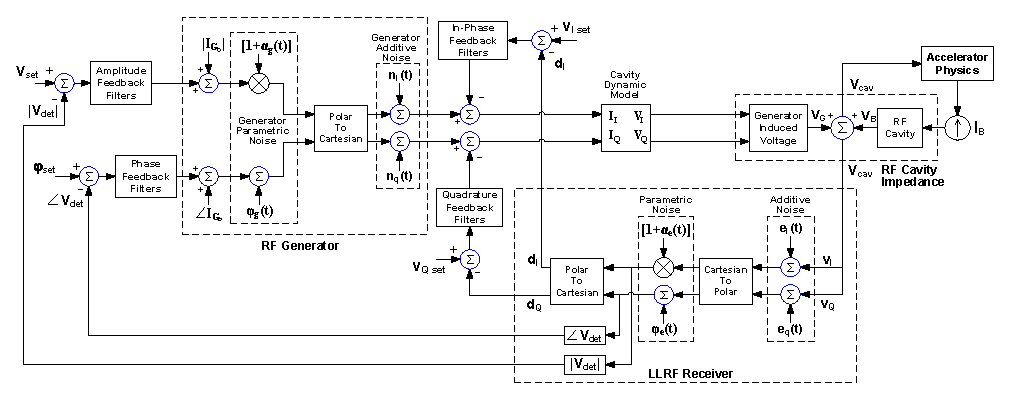
\includegraphics{rfFeedbackModel}
\caption{Rf feedback model used by the {\tt RFMODE} element.}
\label{fig:rfFeedbackModel}
\end{figure}

Normally, the field dumped in the cavity by one particle affects trailing particles in the same turn.
However, if one is also using a \verb|WAKE| or \verb|ZLONGIT| element to simulate the short-range wake of the cavity, this would be double-counting.
In that case, one can use \verb|LONG_RANGE_ONLY=1| to suppress the same-turn effects of the \verb|RFMODE| element.

Two output files are available: the \verb|RECORD| file includes bunch-by-bunch data on the beam-induced fields and the total cavity fields.
The \verb|FEEDBACK_RECORD| file includes tick-by-tick data from the feedback system simulation; {\em writing this file this can significantly impact performance.}

NB: when \verb|BUNCHED_BEAM_MODE| is set to a value other than 1, in order to obtain the effect of several bunches while tracking
only one bunch, the total charge set with the \verb|TOTAL| parameter of the \verb|CHARGE| element should equal the charge in
a single bunch, not the entire beam. However, when \verb|BUNCHED_BEAM_MODE|=1 (allowing an indeterminant number of bunches to be
actually present), then \verb|TOTAL| should be the total for all bunches together.

\vspace*{0.5in}
\input{xyWaveforms.tex}
\newpage
\begin{center}{\Large\verb|RFTM110|}\end{center}
\subsection{RFTM110---Tracks through a TM110-mode (deflecting) rf cavity with all magnetic and electric field components.  NOT RECOMMENDED---See below.}
Tracks through a TM110-mode (deflecting) rf cavity with all magnetic and electric field components.  NOT RECOMMENDED---See below.
\\
Parallel capable? : yes\\
GPU capable? : no\\
Back-tracking capable? : no\\
\begin{tabular}{|l|l|l|l|p{\descwidth}|} \hline
Parameter Name & Units & Type & Default & Description \\ \hline 
PHASE & $DEG$ & double &  0.0 & phase  \\ \hline 
TILT & $RAD$ & double &  0.0 & rotation about longitudinal axis  \\ \hline 
FREQUENCY & $HZ$ & double &   2856000000 & frequency  \\ \hline 
VOLTAGE & $V$ & double &  0.0 & peak deflecting voltage  \\ \hline 
PHASE\_REFERENCE &  & long &  \verb|0| & phase reference number (to link with other time-dependent elements)  \\ \hline 
VOLTAGE\_WAVEFORM &  & STRING &   NULL            & $<$filename$>$=$<$x$>$+$<$y$>$ form specification of input file giving voltage waveform factor vs time  \\ \hline 
VOLTAGE\_PERIODIC &  & short &  \verb|0| & If non-zero, voltage waveform is periodic with period given by time span.  \\ \hline 
ALIGN\_WAVEFORMS &  & short &  \verb|0| & If non-zero, waveforms' t=0 is aligned with first bunch arrival time.  \\ \hline 
VOLTAGE\_NOISE &  & double &  0.0 & Rms fractional noise level for voltage.  \\ \hline 
PHASE\_NOISE & $DEG$ & double &  0.0 & Rms noise level for phase.  \\ \hline 
GROUP\_VOLTAGE\_NOISE &  & double &  0.0 & Rms fractional noise level for voltage linked to group.  \\ \hline 
GROUP\_PHASE\_NOISE & $DEG$ & double &  0.0 & Rms noise level for phase linked to group.  \\ \hline 
VOLTAGE\_NOISE\_GROUP &  & long &  \verb|0| & Group number for voltage noise.  \\ \hline 
PHASE\_NOISE\_GROUP &  & long &  \verb|0| & Group number for phase noise.  \\ \hline 
START\_PASS &  & long &   -1              & If non-negative, pass on which to start modeling cavity.  \\ \hline 
END\_PASS &  & long &   -1              & If non-negative, pass on which to end modeling cavity.  \\ \hline 
GROUP &  & string & NULL & Optionally used to assign an element to a group, with a user-defined name.  Group names will appear in the parameter output file in the column ElementGroup  \\ \hline 
\end{tabular}

\vspace*{0.5in}
\documentclass{article}[12pt]

To derive the field expansion, we start with some results from
Jackson\cite{Jackson}, section 8.7.  The longitudinal electric field
for a TM mode is just
\begin{equation}
E_z = - i E_0 \Psi(\rho, \phi) \cos \left(\frac{p \pi z}{d}\right) e^{-i\omega t},
\end{equation}
where $p$ is an integer, $d$ is the length of the cavity, and we use
cylindrical coordinates $(\rho, \phi, z)$.  The factor of $-i$ represents a
choice of sign and phase convention.  We are interested in the
TM110 mode, so we set $p=0$.  In this case, we have
\begin{equation}
E_x = E_y = 0 
\end{equation}
and (using CGS units)
\begin{equation}
\vec{H} = - i E_0 \frac{i \epsilon \omega}{c k^2} \hat{z} \times \nabla \Psi e^{-i \omega t}.
\end{equation}
For a cylindrical cavity, the function $\Psi$ for the $m=1$ aximuthal mode is 
\begin{equation}
\Psi(\rho, \phi) = J_1 (k \rho) \cos \phi,
\end{equation}
where $k = x_{11}/R$, $x_{11}$ is the first zero of $J_1(x)$, and $R$ is the cavity radius.
We don't need to know the cavity radius, since $k = \omega/c$, where $\omega$ is the
resonant frequency.  By choosing $\cos\phi$ for the aximuthal dependence, we'll get 
a magnetic field primarily in the vertical direction.

In MKS units, the magnetic field is
\begin{equation}
\vec{B} = \frac{E_0}{k c} e^{-i \omega t} \left( \hat{\rho} \frac{J_1(k\rho)}{\rho} \sin \phi
        + \hat{\phi} \cos\phi \frac{\partial J_1(k\rho)}{\partial \rho}\right).
\end{equation}

Using {\tt mathematica}, we expanded these expressions to sixth order
in $k*\rho$.  Here, we present only the expressions to second
order. Taking the real parts only, we now have
\begin{eqnarray}
E_z & \approx & \frac{-1}{2} E_0 k \rho \cos \phi \sin \omega t \\
c B_\rho  & \approx & E_0 \left(\frac{1}{2} - \frac{k^2 \rho^2}{16}\right)\sin\phi \cos\omega t \\
c B_\phi  & \approx & E_0 \left(\frac{1}{2} - \frac{3 k^2 \rho^2}{16}\right)\cos\phi \cos\omega t 
\end{eqnarray}
The Cartesian components of $\vec{B}$ can be computed easily
\begin{eqnarray}
c B_x & = & c B_\rho\cos\phi - c B_\phi\sin\phi \\
      & = & \frac{E_0}{8} \rho^2 k^2 \cos\phi \sin\phi \cos\omega t \\
c B_y & = & c B_\rho\sin\phi + c B_\phi\cos\phi \\
      & = & E_0 \left(\frac{1}{2} - \frac{k^2\rho^2 (2 \cos^2\phi + 1)}{16}\right) \cos\omega t 
\end{eqnarray}

The Lorentz force on an electron is $F = -e E_z \hat{z} - e c \vec{\beta} \times \vec{B}$,
giving
\begin{eqnarray}
F_x/e & = & \beta_z c B_y \\
F_y/e & = & -\beta_z c B_x \\
F_z/e & = & -E_z - \beta_x c B_y + \beta_y c B_x 
\end{eqnarray}
We see that for $\rho \rightarrow 0$, we have $E_z = 0$, $B_x = 0$, and
\begin{equation}
c B_y = \frac{E_0}{2} \cos \omega t.
\end{equation}
Hence, for $\omega t=0$ and $E_0>0$ we have $F_x>0$.  This explains
our choice of sign and phase convention above.

\vspace*{0.5in}
\input{xyWaveforms.tex}
\newpage
\begin{center}{\Large\verb|RFTMEZ0|}\end{center}
\subsection{RFTMEZ0---A TM-mode RF cavity specified by the on-axis Ez field.}
A TM-mode RF cavity specified by the on-axis Ez field.
\\
Parallel capable? : yes\\
GPU capable? : no\\
Back-tracking capable? : no\\
\begin{tabular}{|l|l|l|l|p{\descwidth}|} \hline
Parameter Name & Units & Type & Default & Description \\ \hline 
L & $M$ & double &  0.0 & length  \\ \hline 
FREQUENCY & $HZ$ & double &   2856000000 & frequency  \\ \hline 
PHASE & $RAD$ & double &  0.0 & phase  \\ \hline 
EZ\_PEAK & $V$ & double &  0.0 & Peak on-axis longitudinal electric field  \\ \hline 
TIME\_OFFSET & $S$ & double &  0.0 & time offset (adds to phase)  \\ \hline 
PHASE\_REFERENCE &  & long &  \verb|0| & phase reference number (to link to other time-dependent elements)  \\ \hline 
DX & $M$ & double &  0.0 & misalignment  \\ \hline 
DY & $M$ & double &  0.0 & misalignment  \\ \hline 
DZ & $M$ & double &  0.0 & misalignment  \\ \hline 
ETILT & $RAD$ & double &  0.0 & misalignment  \\ \hline 
EYAW & $RAD$ & double &  0.0 & misalignment  \\ \hline 
EPITCH & $RAD$ & double &  0.0 & misalignment  \\ \hline 
N\_STEPS &  & long &   100             & number of steps (for nonadaptive integration)  \\ \hline 
RADIAL\_ORDER &  & short &   1               & highest order in off-axis expansion  \\ \hline 
CHANGE\_P0 &  & short &  \verb|0| & does element change central momentum?  \\ \hline 
INPUTFILE &  & STRING &   NULL            & file containing Ez vs z at r=0  \\ \hline 
ZCOLUMN &  & STRING &   NULL            & column containing z values  \\ \hline 
EZCOLUMN &  & STRING &   NULL            & column containing Ez values  \\ \hline 
SOLENOID\_FILE &  & STRING &   NULL            & file containing map of Bz and Br vs z and r.  Each page contains values for a single r.  \\ \hline 
SOLENOID\_ZCOLUMN &  & STRING &   NULL            & column containing z values for solenoid map.  \\ \hline 
SOLENOID\_RCOLUMN &  & STRING &   NULL            & column containing r values for solenoid map.  If omitted, data is assumed to be for r=0 and an on-axis expansion is performed.  \\ \hline 
\end{tabular}

\newpage
\begin{center}{\Large\verb|RFTMEZ0| continued}\end{center}
A TM-mode RF cavity specified by the on-axis Ez field.
\\
\begin{tabular}{|l|l|l|l|p{\descwidth}|} \hline
Parameter Name & Units & Type & Default & Description \\ \hline 
SOLENOID\_BZCOLUMN &  & STRING &   NULL            & column containing Bz values for solenoid map.  \\ \hline 
SOLENOID\_BRCOLUMN &  & STRING &   NULL            & column containing Br values for solenoid map. If omitted, data is assumed to be for r=0 and an on-axis expansion is performed.  \\ \hline 
SOLENOID\_FACTOR &  & double &   1 & factor by which to multiply solenoid fields.  \\ \hline 
SOLENOID\_DX & $M$ & double &  0.0 & misalignment  \\ \hline 
SOLENOID\_DY & $M$ & double &  0.0 & misalignment  \\ \hline 
SOLENOID\_DZ & $M$ & double &  0.0 & misalignment  \\ \hline 
SOLENOID\_ETILT & $RAD$ & double &  0.0 & misalignment  \\ \hline 
SOLENOID\_EYAW & $RAD$ & double &  0.0 & misalignment  \\ \hline 
SOLENOID\_EPITCH & $RAD$ & double &  0.0 & misalignment  \\ \hline 
BX\_STRAY &  & double &  0.0 & Uniform stray horizontal field  \\ \hline 
BY\_STRAY &  & double &  0.0 & Uniform stray vertical field  \\ \hline 
ACCURACY &  & double &   0.0001 & integration accuracy  \\ \hline 
METHOD & $ $ & STRING &   runge-kutta     & integration method (runge-kutta, bulirsch-stoer, non-adaptive runge-kutta, modified midpoint)  \\ \hline 
FIDUCIAL &  & STRING &   t,median        & \{t$|$p\},\{median$|$min$|$max$|$ave$|$first$|$light\} (e.g., "t,median")  \\ \hline 
FIELD\_TEST\_FILE &  & STRING &   NULL            & filename for output of test fields (r=0)  \\ \hline 
GROUP &  & string & NULL & Optionally used to assign an element to a group, with a user-defined name.  Group names will appear in the parameter output file in the column ElementGroup  \\ \hline 
\end{tabular}

\newpage
\begin{center}{\Large\verb|RIMULT|}\end{center}
\subsection{RIMULT---Multiplies radiation integrals by a given factor.  Use to compute emittance for collection of various types of cells.}
Multiplies radiation integrals by a given factor.  Use to compute emittance for collection of various types of cells.
\\
Parallel capable? : yes\\
GPU capable? : no\\
Back-tracking capable? : no\\
\begin{tabular}{|l|l|l|l|p{\descwidth}|} \hline
Parameter Name & Units & Type & Default & Description \\ \hline 
FACTOR &  & double &   1 & factor  \\ \hline 
GROUP &  & string & NULL & Optionally used to assign an element to a group, with a user-defined name.  Group names will appear in the parameter output file in the column ElementGroup  \\ \hline 
\end{tabular}

\newpage
\begin{center}{\Large\verb|RMDF|}\end{center}
\subsection{RMDF---A linearly-ramped electric field deflector, using an approximate analytical solution FOR LOW ENERGY PARTICLES.}
A linearly-ramped electric field deflector, using an approximate analytical solution FOR LOW ENERGY PARTICLES.
\\
Parallel capable? : no\\
GPU capable? : no\\
Back-tracking capable? : no\\
\begin{tabular}{|l|l|l|l|p{\descwidth}|} \hline
Parameter Name & Units & Type & Default & Description \\ \hline 
L & $M$ & double &  0.0 & length  \\ \hline 
TILT & $RAD$ & double &  0.0 & rotation about longitudinal axis  \\ \hline 
RAMP\_TIME & $S$ & double &   1e-09 & length of ramp  \\ \hline 
VOLTAGE & $V$ & double &  0.0 & full voltage  \\ \hline 
GAP & $M$ & double &   0.01 & gap between plates  \\ \hline 
TIME\_OFFSET & $S$ & double &  0.0 & time offset of ramp start  \\ \hline 
N\_SECTIONS &  & long &   10              & number of sections  \\ \hline 
PHASE\_REFERENCE &  & long &  \verb|0| & phase reference number (to link with other time-dependent elements)  \\ \hline 
DX & $M$ & double &  0.0 & misalignment  \\ \hline 
DY & $M$ & double &  0.0 & misalignment  \\ \hline 
GROUP &  & string & NULL & Optionally used to assign an element to a group, with a user-defined name.  Group names will appear in the parameter output file in the column ElementGroup  \\ \hline 
\end{tabular}

\newpage
\begin{center}{\Large\verb|ROTATE|}\end{center}
\subsection{ROTATE---An element that rotates the beam about the longitudinal axis.}
An element that rotates the beam about the longitudinal axis.
\\
Parallel capable? : yes\\
GPU capable? : yes\\
Back-tracking capable? : yes\\
\begin{tabular}{|l|l|l|l|p{\descwidth}|} \hline
Parameter Name & Units & Type & Default & Description \\ \hline 
TILT & $RAD$ & double &  0.0 & rotation about longitudinal axis  \\ \hline 
EXCLUDE\_FLOOR &  & short &  \verb|0| & if non-zero, does not affect the floor coordinates  \\ \hline 
EXCLUDE\_OPTICS &  & short &  \verb|0| & if non-zero, does not affect the optics (i.e., transfer matrix is unit matrix)  \\ \hline 
GROUP &  & string & NULL & Optionally used to assign an element to a group, with a user-defined name.  Group names will appear in the parameter output file in the column ElementGroup  \\ \hline 
\end{tabular}

\vspace*{0.5in}
\input{rotate.tex}
\newpage
\begin{center}{\Large\verb|SAMPLE|}\end{center}
\subsection{SAMPLE---An element that reduces the number of particles in the beam by interval-based or random sampling.}
An element that reduces the number of particles in the beam by interval-based or random sampling.
\\
Parallel capable? : yes\\
GPU capable? : no\\
Back-tracking capable? : no\\
\begin{tabular}{|l|l|l|l|p{\descwidth}|} \hline
Parameter Name & Units & Type & Default & Description \\ \hline 
FRACTION &  & double &   1 & fraction to keep  \\ \hline 
INTERVAL &  & long &   1               & interval between sampled particles  \\ \hline 
GROUP &  & string & NULL & Optionally used to assign an element to a group, with a user-defined name.  Group names will appear in the parameter output file in the column ElementGroup  \\ \hline 
\end{tabular}

\newpage
\begin{center}{\Large\verb|SBEN|}\end{center}
\subsection{SBEN---A sector dipole implemented as a matrix, up to 2nd order. Use CSBEND for symplectic tracking.}
A sector dipole implemented as a matrix, up to 2nd order. Use CSBEND for symplectic tracking.
\\
Parallel capable? : yes\\
GPU capable? : yes\\
Back-tracking capable? : yes\\
\begin{tabular}{|l|l|l|l|p{\descwidth}|} \hline
Parameter Name & Units & Type & Default & Description \\ \hline 
L & $M$ & double &  0.0 & arc length  \\ \hline 
ANGLE & $RAD$ & double &  0.0 & bend angle  \\ \hline 
K1 & $1/M^{2}$ & double &  0.0 & geometric focusing strength  \\ \hline 
E1 & $RAD$ & double &  0.0 & entrance edge angle  \\ \hline 
E2 & $RAD$ & double &  0.0 & exit edge angle  \\ \hline 
TILT & $RAD$ & double &  0.0 & rotation about incoming longitudinal axis  \\ \hline 
K2 & $1/M^{3}$ & double &  0.0 & geometric sextupole strength  \\ \hline 
H1 & $1/M$ & double &  0.0 & entrance pole-face curvature  \\ \hline 
H2 & $1/M$ & double &  0.0 & exit pole-face curvature  \\ \hline 
HGAP & $M$ & double &  0.0 & half-gap between poles  \\ \hline 
FINT &  & double &   0.5 & edge-field integral  \\ \hline 
DX & $M$ & double &  0.0 & misaligment of entrance  \\ \hline 
DY & $M$ & double &  0.0 & misalignment of entrance  \\ \hline 
DZ & $M$ & double &  0.0 & misalignment of entrance  \\ \hline 
FSE &  & double &  0.0 & fractional strength error of all components  \\ \hline 
FSE\_DIPOLE &  & double &  0.0 & fractional strength error of dipole component  \\ \hline 
FSE\_QUADRUPOLE &  & double &  0.0 & fractional strength error of quadrupole component  \\ \hline 
ETILT & $RAD$ & double &  0.0 & error rotation about incoming longitudinal axis  \\ \hline 
ETILT\_SIGN &  & short &   -1              & Sign of ETILT relative to TILT. -1 is the old convention and is the default for backwards compatibility  \\ \hline 
EDGE1\_EFFECTS &  & short &   1               & include entrance edge effects?  \\ \hline 
EDGE2\_EFFECTS &  & short &   1               & include exit edge effects?  \\ \hline 
ORDER &  & short &  \verb|0| & matrix order  \\ \hline 
EDGE\_ORDER &  & short &  \verb|0| & edge matrix order  \\ \hline 
TRANSPORT &  & short &  \verb|0| & use (incorrect) TRANSPORT equations for T436 of edge?  \\ \hline 
\end{tabular}

\newpage
\begin{center}{\Large\verb|SBEN| continued}\end{center}
A sector dipole implemented as a matrix, up to 2nd order. Use CSBEND for symplectic tracking.
\\
\begin{tabular}{|l|l|l|l|p{\descwidth}|} \hline
Parameter Name & Units & Type & Default & Description \\ \hline 
USE\_BN &  & short &  \verb|0| & use B1 and B2 instead of K1 and K2 values?  \\ \hline 
B1 & $1/M$ & double &  0.0 & K1 = B1/rho, where rho is bend radius  \\ \hline 
B2 & $1/M^{2}$ & double &  0.0 & K2 = B2/rho  \\ \hline 
GROUP &  & string & NULL & Optionally used to assign an element to a group, with a user-defined name.  Group names will appear in the parameter output file in the column ElementGroup  \\ \hline 
\end{tabular}

\vspace*{0.5in}
{\em Special note about splitting dipoles}: when dipoles are long, it is
common to want to split them into several pieces, to get a better look
at the interior optics.  When doing this, care must be exercised not
to change the optics.  {\tt elegant} has some special features that
are designed to reduce or manage potential problems. At issue is the
need to turn off edge effects between the portions of the same dipole.

First, one can simply use the \verb|divide_elements| command to set up
the splitting.  Using this command, {\tt elegant} takes care of everything.

Second, one can use a series of dipoles {\em with the same name}.  In this case,
elegant automatically turns off interior edge effects.  This is true when the
dipole elements directly follow one another or are separated by a MARK element.

Third, one can use a series of dipoles with different names.  In this case, you
must also use the \verb|EDGE1_EFFECTS| and \verb|EDGE2_EFFECTS| parameters to
turn off interior edge effects.  

\newpage
\begin{center}{\Large\verb|SCATTER|}\end{center}
\subsection{SCATTER---A scattering element to add gaussian random numbers to particle coordinates.}
A scattering element to add gaussian random numbers to particle coordinates.
\\
Parallel capable? : yes\\
GPU capable? : no\\
Back-tracking capable? : no\\
\begin{tabular}{|l|l|l|l|p{\descwidth}|} \hline
Parameter Name & Units & Type & Default & Description \\ \hline 
X & $M$ & double &  0.0 & rms scattering level for x  \\ \hline 
XP &  & double &  0.0 & rms scattering level for x'  \\ \hline 
Y & $M$ & double &  0.0 & rms scattering level for y  \\ \hline 
YP &  & double &  0.0 & rms scattering level for y'  \\ \hline 
DP &  & double &  0.0 & rms scattering level for (p-pCentral)/pCentral  \\ \hline 
PROBABILITY &  & double &   1 & Probability that any particle will be selected for scattering.  \\ \hline 
STARTONPASS &  & long &  \verb|0| & Pass number to start on.  \\ \hline 
ENDONPASS &  & long &   -1              & Pass number to end on (inclusive).  Ignored if negative.  \\ \hline 
GROUP &  & string & NULL & Optionally used to assign an element to a group, with a user-defined name.  Group names will appear in the parameter output file in the column ElementGroup  \\ \hline 
\end{tabular}

\newpage
\begin{center}{\Large\verb|SCMULT|}\end{center}
\subsection{SCMULT---Tracks through a zero length multipole to simulate space charge effects}
Tracks through a zero length multipole to simulate space charge effects
\\
Parallel capable? : yes\\
GPU capable? : no\\
Back-tracking capable? : no\\
\begin{tabular}{|l|l|l|l|p{\descwidth}|} \hline
Parameter Name & Units & Type & Default & Description \\ \hline 
GROUP &  & string & NULL & Optionally used to assign an element to a group, with a user-defined name.  Group names will appear in the parameter output file in the column ElementGroup  \\ \hline 
\end{tabular}

\vspace*{0.5in}
\input{scmult.tex}
\newpage
\begin{center}{\Large\verb|SCRAPER|}\end{center}
\subsection{SCRAPER---A collimating element that sticks into the beam from one side only.  The directions 0, 1, 2, and 3 are from +x, +y, -x, and -y, respectively.}
A collimating element that sticks into the beam from one side only.  The directions 0, 1, 2, and 3 are from +x, +y, -x, and -y, respectively.
\\
Parallel capable? : yes\\
GPU capable? : yes\\
Back-tracking capable? : yes\\
\begin{tabular}{|l|l|l|l|p{\descwidth}|} \hline
Parameter Name & Units & Type & Default & Description \\ \hline 
L & $M$ & double &  0.0 & length  \\ \hline 
XO & $M$ & double &  0.0 & radiation length  \\ \hline 
ENERGY\_DECAY &  & long &  \verb|0| & If nonzero, then particles will lose energy due to material using a simple exponential model.  \\ \hline 
ENERGY\_STRAGGLE &  & long &  \verb|0| & Use simple-minded energy straggling model coupled with ENERGY\_DECAY=1?  \\ \hline 
NUCLEAR\_BREMSSTRAHLUNG &  & long &  \verb|0| & Model energy loss to nuclear bremsstrahlung? If enabled, set ENERGY\_DECAY=0 to disable simpler model.  \\ \hline 
ELECTRON\_RECOIL &  & long &  \verb|0| & If non-zero, electron recoil during Coulomb scattering is included (results in energy change).  \\ \hline 
Z &  & long &  \verb|0| & Atomic number  \\ \hline 
A & $AMU$ & double &  0.0 & Atomic mass  \\ \hline 
RHO & $KG/M^3$ & double &  0.0 & Density  \\ \hline 
PLIMIT &  & double &   0.05 & Probability cutoff for each slice  \\ \hline 
POSITION & $M$ & double &  0.0 & position of edge  \\ \hline 
DX & $M$ & double &  0.0 & misalignment  \\ \hline 
DY & $M$ & double &  0.0 & misalignment  \\ \hline 
INSERT\_FROM &  & STRING &   NULL            & direction from which inserted (+x, -x, x, +y, -y, y)  \\ \hline 
DIRECTION &  & long &   -1              & Deprecated. use INSERT\_FROM.  \\ \hline 
GROUP &  & string & NULL & Optionally used to assign an element to a group, with a user-defined name.  Group names will appear in the parameter output file in the column ElementGroup  \\ \hline 
\end{tabular}

\vspace*{0.5in}
The method used for material modeling is the same as that used for the \verb|MATTER| element.

\newpage
\begin{center}{\Large\verb|SCRIPT|}\end{center}
\subsection{SCRIPT---An element that allows transforming the beam using an external script.}
An element that allows transforming the beam using an external script.
\\
Parallel capable? : yes\\
GPU capable? : no\\
Back-tracking capable? : yes\\
\begin{tabular}{|l|l|l|l|p{\descwidth}|} \hline
Parameter Name & Units & Type & Default & Description \\ \hline 
L & $M$ & double &  0.0 & Length to be used for matrix-based operations such as twiss parameter computation.  \\ \hline 
COMMAND &  & STRING &   NULL            & SDDS-compliant command to apply to the beam.  Use the sequence \%i to represent the input filename and \%o to represent the output filename.  \\ \hline 
USE\_CSH &  & short &   1               & Use C-shell for execution (may be slower)?  \\ \hline 
VERBOSITY &  & short &  \verb|0| & Set the verbosity level.  \\ \hline 
RPN\_PARAMETERS &  & short &  \verb|0| & If nonzero, then parameters from the script output file are loaded into RPN variables.  \\ \hline 
START\_PASS &  & long &   -1              & Start script action on this pass.  Before that, behaves like a drift space.  \\ \hline 
END\_PASS &  & long &   -1              & End script action after this pass.  Before that, behaves like a drift space.  \\ \hline 
PASS\_INTERVAL &  & long &   -1              & Execute script only every Nth pass following START\_PASS, including START\_PASS. Otherwise, behaves like a drift space.  \\ \hline 
ON\_PASS &  & long &   -1              & Perform script action only on this pass, overriding other pass controls. Other than that, behaves like a drift space.  \\ \hline 
DIRECTORY &  & STRING &   NULL            & Directory in which to place input and output files.  If blank, the present working directory is used.  \\ \hline 
ROOTNAME &  & STRING &   NULL            & Rootname for use in naming input and output files.  \%s may be used to represent the run rootname.  \\ \hline 
\end{tabular}

\newpage
\begin{center}{\Large\verb|SCRIPT| continued}\end{center}
An element that allows transforming the beam using an external script.
\\
\begin{tabular}{|l|l|l|l|p{\descwidth}|} \hline
Parameter Name & Units & Type & Default & Description \\ \hline 
INPUT\_EXTENSION &  & STRING &   in              & Extension for the script input file.  \\ \hline 
OUTPUT\_EXTENSION &  & STRING &   out             & Extension for the script output file.  \\ \hline 
KEEP\_FILES &  & short &  \verb|0| & If nonzero, then script input and output files are not deleted after use.  By default, they are deleted.  \\ \hline 
DRIFT\_MATRIX &  & short &  \verb|0| & If nonzero, then for non-tracking calculations the element is treated as a drift space.  \\ \hline 
USE\_PARTICLE\_ID &  & short &   1               & If nonzero, then the output file will supply particle IDs. Otherwise, particles are renumbered.  \\ \hline 
NO\_NEW\_PARTICLES &  & short &   1               & If nonzero, then no new particles will be added in the script output file.  \\ \hline 
DETERMINE\_LOSSES\_FROM\_PID &  & short &   1               & If nonzero and if USE\_PARTICLE\_ID is nonzero, then particleID data from script output is used to determine which particles were lost.  \\ \hline 
SOFT\_FAILURE &  & short &   1               & If output file does not exist or can't be read, consider all particles lost.  \\ \hline 
NP0 &  & double &  0.0 & User-defined numerical parameter for command substitution for sequence \%np0  \\ \hline 
NP1 &  & double &  0.0 & User-defined numerical parameter for command substitution for sequence \%np1  \\ \hline 
NP2 &  & double &  0.0 & User-defined numerical parameter for command substitution for sequence \%np2  \\ \hline 
\end{tabular}

\newpage
\begin{center}{\Large\verb|SCRIPT| continued}\end{center}
An element that allows transforming the beam using an external script.
\\
\begin{tabular}{|l|l|l|l|p{\descwidth}|} \hline
Parameter Name & Units & Type & Default & Description \\ \hline 
NP3 &  & double &  0.0 & User-defined numerical parameter for command substitution for sequence \%np3  \\ \hline 
NP4 &  & double &  0.0 & User-defined numerical parameter for command substitution for sequence \%np4  \\ \hline 
NP5 &  & double &  0.0 & User-defined numerical parameter for command substitution for sequence \%np5  \\ \hline 
NP6 &  & double &  0.0 & User-defined numerical parameter for command substitution for sequence \%np6  \\ \hline 
NP7 &  & double &  0.0 & User-defined numerical parameter for command substitution for sequence \%np7  \\ \hline 
NP8 &  & double &  0.0 & User-defined numerical parameter for command substitution for sequence \%np8  \\ \hline 
NP9 &  & double &  0.0 & User-defined numerical parameter for command substitution for sequence \%np9  \\ \hline 
SP0 &  & STRING &   NULL            & User-defined string parameter for command substitution for sequence \%sp0  \\ \hline 
SP1 &  & STRING &   NULL            & User-defined string parameter for command substitution for sequence \%sp1  \\ \hline 
SP2 &  & STRING &   NULL            & User-defined string parameter for command substitution for sequence \%sp2  \\ \hline 
SP3 &  & STRING &   NULL            & User-defined string parameter for command substitution for sequence \%sp3  \\ \hline 
SP4 &  & STRING &   NULL            & User-defined string parameter for command substitution for sequence \%sp4  \\ \hline 
\end{tabular}

\newpage
\begin{center}{\Large\verb|SCRIPT| continued}\end{center}
An element that allows transforming the beam using an external script.
\\
\begin{tabular}{|l|l|l|l|p{\descwidth}|} \hline
Parameter Name & Units & Type & Default & Description \\ \hline 
SP5 &  & STRING &   NULL            & User-defined string parameter for command substitution for sequence \%sp5  \\ \hline 
SP6 &  & STRING &   NULL            & User-defined string parameter for command substitution for sequence \%sp6  \\ \hline 
SP7 &  & STRING &   NULL            & User-defined string parameter for command substitution for sequence \%sp7  \\ \hline 
SP8 &  & STRING &   NULL            & User-defined string parameter for command substitution for sequence \%sp8  \\ \hline 
SP9 &  & STRING &   NULL            & User-defined string parameter for command substitution for sequence \%sp9  \\ \hline 
GROUP &  & string & NULL & Optionally used to assign an element to a group, with a user-defined name.  Group names will appear in the parameter output file in the column ElementGroup  \\ \hline 
\end{tabular}

\vspace*{0.5in}
\input{script.tex}
\newpage
\begin{center}{\Large\verb|SEXT|}\end{center}
\subsection{SEXT---A sextupole implemented as a matrix, up to 3rd order. Use KSEXT for symplectic tracking.}
A sextupole implemented as a matrix, up to 3rd order. Use KSEXT for symplectic tracking.
\\
Parallel capable? : yes\\
GPU capable? : yes\\
Back-tracking capable? : yes\\
\begin{tabular}{|l|l|l|l|p{\descwidth}|} \hline
Parameter Name & Units & Type & Default & Description \\ \hline 
L & $M$ & double &  0.0 & length  \\ \hline 
K2 & $1/M^{3}$ & double &  0.0 & geometric strength  \\ \hline 
K1 & $1/M^{2}$ & double &  0.0 & geometric quadrupole strength error. See notes below!  \\ \hline 
J1 & $1/M^{2}$ & double &  0.0 & geometric skew quadrupole strength error. See notes below!  \\ \hline 
TILT & $RAD$ & double &  0.0 & rotation about longitudinal axis  \\ \hline 
DX & $M$ & double &  0.0 & misalignment  \\ \hline 
DY & $M$ & double &  0.0 & misalignment  \\ \hline 
DZ & $M$ & double &  0.0 & misalignment  \\ \hline 
FSE &  & double &  0.0 & fractional strength error  \\ \hline 
FFRINGE &  & double &  0.0 & Length occupied by linear fringe regions as fraction hard-edge length L.  \\ \hline 
ORDER &  & short &  \verb|0| & matrix order  \\ \hline 
GROUP &  & string & NULL & Optionally used to assign an element to a group, with a user-defined name.  Group names will appear in the parameter output file in the column ElementGroup  \\ \hline 
\end{tabular}

\vspace*{0.5in}
This element simulates a sextupole using a matrix, up to third order.

The \verb|K1| and \verb|J1| parameters allow introducing normal and skew quadrupole {\bf error} terms.
The matrix expressions assume that
these are weak effects and high accuracy should not be expected if this is not true.
If \verb|K1| is significant, then use of the \verb|KQUSE| element is preferred.


\newpage
\begin{center}{\Large\verb|SHRFDF|}\end{center}
\subsection{SHRFDF---Simulation through space harmonics of zero length deflecting cavity.}
Simulation through space harmonics of zero length deflecting cavity.
\\
Parallel capable? : yes\\
GPU capable? : no\\
Back-tracking capable? : no\\
\begin{tabular}{|l|l|l|l|p{\descwidth}|} \hline
Parameter Name & Units & Type & Default & Description \\ \hline 
FACTOR &  & double &   1 & A factor by which to multiply all components.  \\ \hline 
TILT & $RAD$ & double &  0.0 & rotation about longitudinal axis  \\ \hline 
PERIOD\_LENGTH & $M$ & double &  0.0 & cavity period length, or cell length  \\ \hline 
PERIOD\_PHASE & $RAD$ & double &  0.0 & cavity period phase advance, or so-called working mode  \\ \hline 
V0 & $V$ & double &  0.0 & effective voltage of space harmonic n=0  \\ \hline 
V1 & $V$ & double &  0.0 & effective voltage of space harmonic n=1  \\ \hline 
V2 & $V$ & double &  0.0 & effective voltage of space harmonic n=2  \\ \hline 
V3 & $V$ & double &  0.0 & effective voltage of space harmonic n=3  \\ \hline 
V4 & $V$ & double &  0.0 & effective voltage of space harmonic n=4  \\ \hline 
V5 & $V$ & double &  0.0 & effective voltage of space harmonic n=5  \\ \hline 
V6 & $V$ & double &  0.0 & effective voltage of space harmonic n=6  \\ \hline 
V7 & $V$ & double &  0.0 & effective voltage of space harmonic n=7  \\ \hline 
V8 & $V$ & double &  0.0 & effective voltage of space harmonic n=8  \\ \hline 
V9 & $V$ & double &  0.0 & effective voltage of space harmonic n=9  \\ \hline 
PHASE0 & $HZ$ & double &  0.0 & Phase of space harmonic n=0  \\ \hline 
PHASE1 & $HZ$ & double &  0.0 & Phase of space harmonic n=1  \\ \hline 
PHASE2 & $HZ$ & double &  0.0 & Phase of space harmonic n=2  \\ \hline 
PHASE3 & $HZ$ & double &  0.0 & Phase of space harmonic n=3  \\ \hline 
PHASE4 & $HZ$ & double &  0.0 & Phase of space harmonic n=4  \\ \hline 
PHASE5 & $HZ$ & double &  0.0 & Phase of space harmonic n=5  \\ \hline 
PHASE6 & $HZ$ & double &  0.0 & Phase of space harmonic n=6  \\ \hline 
PHASE7 & $HZ$ & double &  0.0 & Phase of space harmonic n=7  \\ \hline 
\end{tabular}

\newpage
\begin{center}{\Large\verb|SHRFDF| continued}\end{center}
Simulation through space harmonics of zero length deflecting cavity.
\\
\begin{tabular}{|l|l|l|l|p{\descwidth}|} \hline
Parameter Name & Units & Type & Default & Description \\ \hline 
PHASE8 & $HZ$ & double &  0.0 & Phase of space harmonic n=8  \\ \hline 
PHASE9 & $HZ$ & double &  0.0 & Phase of space harmonic n=9  \\ \hline 
PHASE\_REFERENCE &  & long &  \verb|0| & phase reference number (to link with other time-dependent elements)  \\ \hline 
GROUP &  & string & NULL & Optionally used to assign an element to a group, with a user-defined name.  Group names will appear in the parameter output file in the column ElementGroup  \\ \hline 
\end{tabular}

\vspace*{0.5in}
This element simulates an rf deflector with specified space harmonic parameters (voltage, phase).
The thin kicks from the fundamental deflecting mode are the same as for the element RFDF. The thin kicks from the space
harmonics ($n\ge 1$) are \cite{Sun-NAPAC19}

\begin{equation}
\renewcommand{\arraystretch}{1.5}
\begin{array}{lcl}
\Delta P_x & = & -\frac{\partial ({\bf H} - H_0)}{\partial x} \\
  &  = & \sum\limits_{n=1}^{\infty} -q \bar{ V_n} \cdot \sin (k_n z + \phi_n) \cdot (\frac{1}{2}\alpha_n + \frac{1}{16}\alpha_n^3 \cdot (3x^2 + y^2)) \\
\end{array}
\end{equation}

\begin{equation}
\renewcommand{\arraystretch}{1.5}
\begin{array}{lcl}
\Delta P_z & = & -\frac{\partial ({\bf H} - H_0)}{\partial z} \\
           & = & \sum\limits_{n=1}^{\infty} -q \bar{ V_n} \cdot k_n \cdot \cos (k_n z + \phi_n) 
           \cdot (\frac{1}{2}\alpha_n \cdot x + \frac{1}{16}\alpha_n^3 \cdot (x^2 + y^2)\cdot x)\\
\end{array}
\end{equation} 

The wave numbers $k_n$ and $\alpha_n$ are listed below.
\begin{equation}\label{Equa1}
k_n = \frac{\varphi_0 + 2\pi n}{d}
\end{equation} 
\begin{equation}\label{Equa1}
\alpha_n^2 + k_n^2 = k_0^2
\end{equation} 
where $k_n$ is wave number of $n^{th}$ space harmonic, $n$ an integer number, $\varphi_0$ the phase advance per cavity
period, $d$ the cavity period length, $\alpha_n$ the wave number in the radial direction, $m$ wave number (per $2\pi$)
in the angular direction.


\newpage
\begin{center}{\Large\verb|SLICE|}\end{center}
\subsection{SLICE---Performs slice-by-slice analysis of the beam for output to a file.}
Performs slice-by-slice analysis of the beam for output to a file.
\\
Parallel capable? : yes\\
GPU capable? : no\\
Back-tracking capable? : no\\
\begin{tabular}{|l|l|l|l|p{\descwidth}|} \hline
Parameter Name & Units & Type & Default & Description \\ \hline 
N\_SLICES &  & long &   10              & number of slices  \\ \hline 
START\_PID &  & long &   -1              & starting particleID for particles to dump  \\ \hline 
END\_PID &  & long &   -1              & ending particleID for particles to dump  \\ \hline 
INTERVAL &  & long &   1               & interval for data output (in turns)  \\ \hline 
START\_PASS &  & long &  \verb|0| & pass on which to start  \\ \hline 
END\_PASS &  & long &   -1              & pass on which to end (inclusive).  Ignored if negative.  \\ \hline 
FILENAME &  & STRING &                   & output filename, possibly incomplete (see below)  \\ \hline 
LABEL &  & STRING &                   & output label  \\ \hline 
INDEX\_OFFSET &  & long &  \verb|0| & Offset for file indices for sequential file naming.  \\ \hline 
REFERENCE\_FREQUENCY &  & double &   -1 & If non-zero, the indicated frequency is used to define the bucket center for purposes of computing time offsets.  \\ \hline 
DISABLE &  & short &  \verb|0| & If nonzero, no output will be generated.  \\ \hline 
USE\_DISCONNECT &  & short &  \verb|0| & If nonzero, files are disconnected between each write operation. May be useful for parallel operation.  Ignored otherwise.  \\ \hline 
GROUP &  & string & NULL & Optionally used to assign an element to a group, with a user-defined name.  Group names will appear in the parameter output file in the column ElementGroup  \\ \hline 
\end{tabular}

\vspace*{0.5in}
NB: This element has very poor parallel efficiency. Hence, the \verb|START_PASS|, \verb|END_PASS|, and
\verb|INTERVAL| options should be used to limit the frequency of computations to the minimum needed.

\newpage
\begin{center}{\Large\verb|SOLE|}\end{center}
\subsection{SOLE---A solenoid implemented as a matrix, up to 2nd order.}
A solenoid implemented as a matrix, up to 2nd order.
\\
Parallel capable? : yes\\
GPU capable? : yes\\
Back-tracking capable? : yes\\
\begin{tabular}{|l|l|l|l|p{\descwidth}|} \hline
Parameter Name & Units & Type & Default & Description \\ \hline 
L & $M$ & double &  0.0 & length  \\ \hline 
KS & $RAD/M$ & double &  0.0 & geometric strength, -Bs/(B*Rho)  \\ \hline 
B & $T$ & double &  0.0 & field strength (used if KS is zero)  \\ \hline 
DX & $M$ & double &  0.0 & misalignment  \\ \hline 
DY & $M$ & double &  0.0 & misalignment  \\ \hline 
DZ & $M$ & double &  0.0 & misalignment  \\ \hline 
ORDER &  & short &  \verb|0| & matrix order  \\ \hline 
GROUP &  & string & NULL & Optionally used to assign an element to a group, with a user-defined name.  Group names will appear in the parameter output file in the column ElementGroup  \\ \hline 
\end{tabular}

\newpage
\begin{center}{\Large\verb|SPEEDBUMP|}\end{center}
\subsection{SPEEDBUMP---Simulates a semi-circular protuberance from one or both walls of the chamber.}
Simulates a semi-circular protuberance from one or both walls of the chamber.
\\
Parallel capable? : yes\\
GPU capable? : no\\
Back-tracking capable? : no\\
\begin{tabular}{|l|l|l|l|p{\descwidth}|} \hline
Parameter Name & Units & Type & Default & Description \\ \hline 
L & $M$ & double &  0.0 & insertion length  \\ \hline 
CHORD & $M$ & double &  0.0 & z length of speed bump  \\ \hline 
DZCENTER & $M$ & double &  0.0 & z center displacement of speed bump relative to middle of object  \\ \hline 
HEIGHT & $M$ & double &  0.0 & height above the surrounding chamber  \\ \hline 
POSITION & $M$ & double &  0.0 & position of peak relative to ideal trajectory  \\ \hline 
DX & $M$ & double &  0.0 & horizontal misalignment  \\ \hline 
DY & $M$ & double &  0.0 & vertical misalignment  \\ \hline 
INSERT\_FROM &  & STRING &   NULL            & direction from which inserted (x, +x, -x, y, +y, -y)  \\ \hline 
GROUP &  & string & NULL & Optionally used to assign an element to a group, with a user-defined name.  Group names will appear in the parameter output file in the column ElementGroup  \\ \hline 
\end{tabular}

\vspace*{0.5in}
This element simulates a commonplace type of aperture restriction, consisting of a
bump on one or both sides of a chamber. The parameters of the speedbump are
illustrated in Fig. \ref{fig:speedbump}

\begin{figure}[htb]
\center
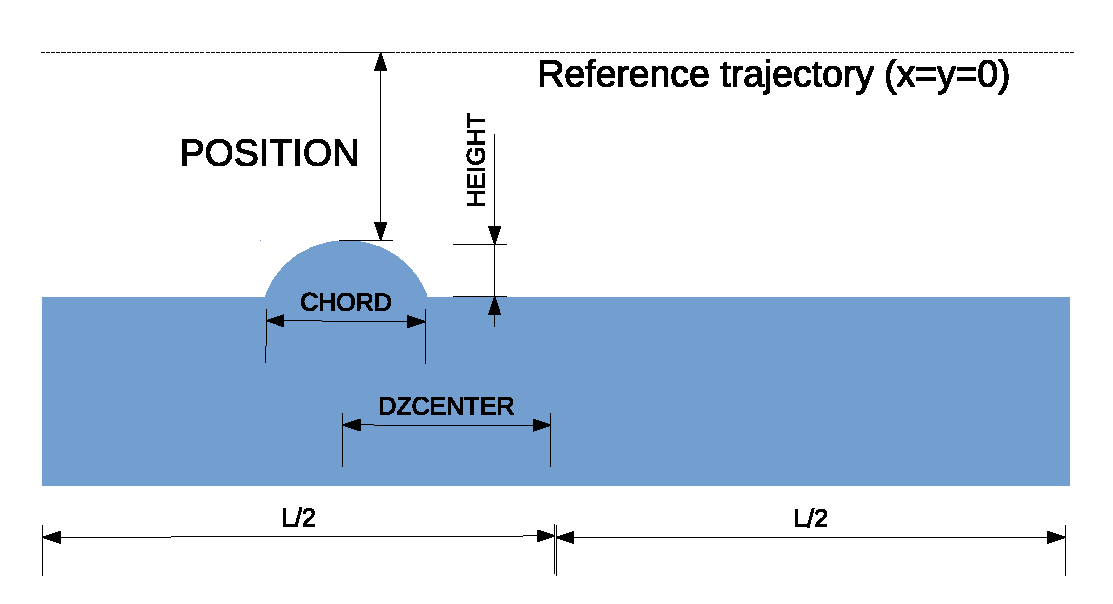
\includegraphics[width=0.8\linewidth]{speedbump}
\caption{Illustration of the parameters used in specifying a speedbump.}
\label{fig:speedbump}
\end{figure}

\clearpage

\newpage
\begin{center}{\Large\verb|SREFFECTS|}\end{center}
\subsection{SREFFECTS---Lumped simulation of synchrotron radiation effects (damping and quantum excitation) for rings.}
Lumped simulation of synchrotron radiation effects (damping and quantum excitation) for rings.
\\
Parallel capable? : yes\\
GPU capable? : no\\
Back-tracking capable? : no\\
\begin{tabular}{|l|l|l|l|p{\descwidth}|} \hline
Parameter Name & Units & Type & Default & Description \\ \hline 
JX &  & double &   1 & x damping partition number  \\ \hline 
JY &  & double &   1 & y damping partition number  \\ \hline 
JDELTA &  & double &   2 & momentum damping partition number  \\ \hline 
EXREF & $m$ & double &  0.0 & reference equilibrium x emittance  \\ \hline 
EYREF & $m$ & double &  0.0 & reference equilibrium y emittance  \\ \hline 
SDELTAREF &  & double &  0.0 & reference equilibrium fractional momentum spread  \\ \hline 
DDELTAREF &  & double &  0.0 & reference fractional momentum change per turn due to SR (negative value)  \\ \hline 
PREF & $m_{e}c$ & double &  0.0 & reference momentum (to which other reference values pertain)  \\ \hline 
COUPLING &  & double &  0.0 & x-y coupling  \\ \hline 
FRACTION &  & double &   1 & fraction of implied SR effect to simulate with each instance  \\ \hline 
DAMPING &  & long &   1               & include damping, less rf effects?  \\ \hline 
QEXCITATION &  & long &   1               & include quantum excitation?  \\ \hline 
LOSSES &  & long &   1               & include average losses?  \\ \hline 
CUTOFF &  & double &   100 & cutoff (in sigmas) for gaussian random numbers  \\ \hline 
INCLUDE\_OFFSETS &  & long &   1               & include orbit offsets in tracking (see below)?  \\ \hline 
GROUP &  & string & NULL & Optionally used to assign an element to a group, with a user-defined name.  Group names will appear in the parameter output file in the column ElementGroup  \\ \hline 
\end{tabular}

\vspace*{0.5in}
This element allows simulation of synchrotron radiation effects in a
lumped fashion for quick, approximate results.  There are two ways to
set up the element: explicit initialization or automatic
initialization.  

In explicit initialization, the user supplies the quantities {\tt
EXREF}, {\tt EYREF}, {\tt SDELTAREF}, {\tt DDELTAREF}, and {\tt
PREF}.  These are, respectively, the reference values for the x-plane
emittance, y-plane emittance, fractional momentum spread, energy loss
per turn, and momentum.  The first four values pertain to the
reference momentum.  {\tt JX}, {\tt JY}, and {\tt JDELTA} may also
be given, although the defaults work for typical lattices.

In automatic initialization, the user turns on the radiation integral
feature in {\tt twiss\_output}, causing {\tt elegant} to automatically
compute the above quantities.  This will occur only if {\tt PREF=0}.
The {\tt COUPLING} parameter can be used to change the partitioning of
quantum excitation between the horizontal and vertical planes.

In versions 19.0 and later, {\tt elegant} includes the effect of {\tt
SREFFECTS} on the closed orbit.  This presents a dilemna when
automatic initialization is used, because in order to perform
automatic initialization, {\tt elegant} has to compute the optics
functions.  However, it must determine the closed orbit to compute the
optics functions.  The solution to this is for the user to pre-compute
the twiss parameters and radiation integrals using \verb|twiss_output|
with \verb|output_at_each_step=0|.  The user is free to subsequently give
\verb|twiss_output| with \verb|output_at_each_step=1| to obtain the
results on the closed orbit.

N.B.: Computation of Twiss parameters does not fully include the
effects of synchrotron radiation losses when these are imposed using
{\tt SREFFECTS} elements.  If {\tt PREF=0} (automatic initialization),
these effects are completely missing.  If {\tt PREF} is non-zero, then
{\tt elegant} will use the {\tt DDELTAREF} parameter to compute the
energy offset from the element, and thus its effect on the beam
trajectory.




\newpage
\begin{center}{\Large\verb|STRAY|}\end{center}
\subsection{STRAY---A stray field element with local and global components.  Global components are defined relative to the initial beamline direction.}
A stray field element with local and global components.  Global components are defined relative to the initial beamline direction.
\\
Parallel capable? : yes\\
GPU capable? : no\\
Back-tracking capable? : no\\
\begin{tabular}{|l|l|l|l|p{\descwidth}|} \hline
Parameter Name & Units & Type & Default & Description \\ \hline 
L & $M$ & double &  0.0 & length  \\ \hline 
LBX & $T$ & double &  0.0 & local Bx  \\ \hline 
LBY & $T$ & double &  0.0 & local By  \\ \hline 
GBX & $T$ & double &  0.0 & global Bx  \\ \hline 
GBY & $T$ & double &  0.0 & global By  \\ \hline 
GBZ & $T$ & double &  0.0 & global Bz  \\ \hline 
ORDER &  & long &  \verb|0| & matrix order  \\ \hline 
GROUP &  & string & NULL & Optionally used to assign an element to a group, with a user-defined name.  Group names will appear in the parameter output file in the column ElementGroup  \\ \hline 
\end{tabular}

\vspace*{0.5in}
\input{stray.tex}
\newpage
\begin{center}{\Large\verb|TAPERAPC|}\end{center}
\subsection{TAPERAPC---A tapered aperture that is a section of a circular cylinder.}
A tapered aperture that is a section of a circular cylinder.
\\
Parallel capable? : yes\\
GPU capable? : no\\
Back-tracking capable? : no\\
\begin{tabular}{|l|l|l|l|p{\descwidth}|} \hline
Parameter Name & Units & Type & Default & Description \\ \hline 
L & $M$ & double &  0.0 & length  \\ \hline 
RSTART & $M$ & double &  0.0 & radius at the start  \\ \hline 
REND & $M$ & double &  0.0 & radius at the end  \\ \hline 
DX & $M$ & double &  0.0 & misalignment  \\ \hline 
DY & $M$ & double &  0.0 & misalignment  \\ \hline 
STICKY & $NULL$ & short &  \verb|0| & final aperture holds downstream until next TAPERAPC, TAPERAPE, TAPERAPR, or MAXAMP  \\ \hline 
GROUP &  & string & NULL & Optionally used to assign an element to a group, with a user-defined name.  Group names will appear in the parameter output file in the column ElementGroup  \\ \hline 
\end{tabular}

\newpage
\begin{center}{\Large\verb|TAPERAPE|}\end{center}
\subsection{TAPERAPE---A tapered elliptical aperture.}
A tapered elliptical aperture.
\\
Parallel capable? : yes\\
GPU capable? : no\\
Back-tracking capable? : no\\
\begin{tabular}{|l|l|l|l|p{\descwidth}|} \hline
Parameter Name & Units & Type & Default & Description \\ \hline 
L & $M$ & double &  0.0 & length  \\ \hline 
ASTART & $M$ & double &  0.0 & horizontal semi-axis at the start  \\ \hline 
AEND & $M$ & double &  0.0 & horizontal semi-axis at the end  \\ \hline 
BSTART & $M$ & double &  0.0 & vertical semi-axis at the start  \\ \hline 
BEND & $M$ & double &  0.0 & vertical semi-axis at the end  \\ \hline 
DX & $M$ & double &  0.0 & misalignment  \\ \hline 
DY & $M$ & double &  0.0 & misalignment  \\ \hline 
TILT & $RAD$ & double &  0.0 & misalignment  \\ \hline 
RESOLUTION & $M$ & double &   1e-06 & z resolution of finding intersection  \\ \hline 
XEXPONENT & $NULL$ & short &   2               & super-elliptical exponent (even number)  \\ \hline 
YEXPONENT & $NULL$ & short &   2               & super-elliptical exponent (even number)  \\ \hline 
STICKY & $NULL$ & short &  \verb|0| & final aperture holds downstream until next TAPERAPC, TAPERAPE, TAPERAPR, or MAXAMP  \\ \hline 
GROUP &  & string & NULL & Optionally used to assign an element to a group, with a user-defined name.  Group names will appear in the parameter output file in the column ElementGroup  \\ \hline 
\end{tabular}

\newpage
\begin{center}{\Large\verb|TAPERAPR|}\end{center}
\subsection{TAPERAPR---A tapered rectangular aperture.}
A tapered rectangular aperture.
\\
Parallel capable? : yes\\
GPU capable? : no\\
Back-tracking capable? : no\\
\begin{tabular}{|l|l|l|l|p{\descwidth}|} \hline
Parameter Name & Units & Type & Default & Description \\ \hline 
L & $M$ & double &  0.0 & length  \\ \hline 
XSTART & $M$ & double &  0.0 & horizontal half-aperture at the start  \\ \hline 
XEND & $M$ & double &  0.0 & horizontal half-aperture at the end  \\ \hline 
YSTART & $M$ & double &  0.0 & vertical half-aperture at the start  \\ \hline 
YEND & $M$ & double &  0.0 & vertical half-aperture at the end  \\ \hline 
DX & $M$ & double &  0.0 & misalignment  \\ \hline 
DY & $M$ & double &  0.0 & misalignment  \\ \hline 
TILT & $RAD$ & double &  0.0 & misalignment  \\ \hline 
STICKY & $NULL$ & short &  \verb|0| & final aperture holds downstream until next TAPERAPC, TAPERAPE, TAPERAPR, or MAXAMP  \\ \hline 
GROUP &  & string & NULL & Optionally used to assign an element to a group, with a user-defined name.  Group names will appear in the parameter output file in the column ElementGroup  \\ \hline 
\end{tabular}

\newpage
\begin{center}{\Large\verb|TFBDRIVER|}\end{center}
\subsection{TFBDRIVER---Driver for a turn-by-turn feedback loop}
Driver for a turn-by-turn feedback loop
\\
Parallel capable? : yes\\
GPU capable? : no\\
Back-tracking capable? : no\\
\begin{tabular}{|l|l|l|l|p{\descwidth}|} \hline
Parameter Name & Units & Type & Default & Description \\ \hline 
ID &  & STRING &   NULL            & System identifier  \\ \hline 
STRENGTH &  & double &  0.0 & Strength factor  \\ \hline 
KICK\_LIMIT &  & double &  0.0 & Limit on applied kick, nominally in radians.  \\ \hline 
FREQUENCY & $Hz$ & double &  0.0 & Resonant frequency of the unloaded kicker cavity.  \\ \hline 
DRIVE\_FREQUENCY & $Hz$ & double &  0.0 & Drive frequency. If zero, defaults to resonant frequency of the loaded cavity.  \\ \hline 
CLOCK\_FREQUENCY & $Hz$ & double &  0.0 & Clock frequency used for timing of the changes to generator current. Typically the rf or bunch frequency is used.  \\ \hline 
CLOCK\_OFFSET & $s$ & double &  0.0 & Offset of the generator current change relative to clock tick. Clock tick is nominally aligned to the bunch center.  \\ \hline 
PHASE & $Deg$ & double &  0.0 & Phase of the applied voltage relative to the bunch center, with 0 being on-crest.  \\ \hline 
RAOVERQ & $Ohm$ & double &  0.0 & Shunt impedance, Ra/Q=V\^2/(P*Q).  \\ \hline 
QLOADED &  & double &  0.0 & Loaded Q of the cavity.  \\ \hline 
OUTPUT\_FILE &  & STRING &   NULL            & File for logging filter output and driver output  \\ \hline 
GAIN\_FACTOR\_FILE &  & STRING &   NULL            & File providing gain factors for individual bunches.  \\ \hline 
GAIN\_FACTOR\_COLUMN &  & STRING &   NULL            & Column from GAIN\_FACTOR\_FILE containing gain factors.  \\ \hline 
DELAY &  & long &  \verb|0| & Delay (in turns)  \\ \hline 
A0 &  & double &   1 & Filter coefficient  \\ \hline 
A1 &  & double &  0.0 & Filter coefficient  \\ \hline 
A2 &  & double &  0.0 & Filter coefficient  \\ \hline 
A3 &  & double &  0.0 & Filter coefficient  \\ \hline 
\end{tabular}

\newpage
\begin{center}{\Large\verb|TFBDRIVER| continued}\end{center}
Driver for a turn-by-turn feedback loop
\\
\begin{tabular}{|l|l|l|l|p{\descwidth}|} \hline
Parameter Name & Units & Type & Default & Description \\ \hline 
A4 &  & double &  0.0 & Filter coefficient  \\ \hline 
A5 &  & double &  0.0 & Filter coefficient  \\ \hline 
A6 &  & double &  0.0 & Filter coefficient  \\ \hline 
A7 &  & double &  0.0 & Filter coefficient  \\ \hline 
A8 &  & double &  0.0 & Filter coefficient  \\ \hline 
A9 &  & double &  0.0 & Filter coefficient  \\ \hline 
A10 &  & double &  0.0 & Filter coefficient  \\ \hline 
A11 &  & double &  0.0 & Filter coefficient  \\ \hline 
A12 &  & double &  0.0 & Filter coefficient  \\ \hline 
A13 &  & double &  0.0 & Filter coefficient  \\ \hline 
A14 &  & double &  0.0 & Filter coefficient  \\ \hline 
A15 &  & double &  0.0 & Filter coefficient  \\ \hline 
A16 &  & double &  0.0 & Filter coefficient  \\ \hline 
A17 &  & double &  0.0 & Filter coefficient  \\ \hline 
A18 &  & double &  0.0 & Filter coefficient  \\ \hline 
A19 &  & double &  0.0 & Filter coefficient  \\ \hline 
A20 &  & double &  0.0 & Filter coefficient  \\ \hline 
A21 &  & double &  0.0 & Filter coefficient  \\ \hline 
A22 &  & double &  0.0 & Filter coefficient  \\ \hline 
A23 &  & double &  0.0 & Filter coefficient  \\ \hline 
A24 &  & double &  0.0 & Filter coefficient  \\ \hline 
A25 &  & double &  0.0 & Filter coefficient  \\ \hline 
A26 &  & double &  0.0 & Filter coefficient  \\ \hline 
A27 &  & double &  0.0 & Filter coefficient  \\ \hline 
A28 &  & double &  0.0 & Filter coefficient  \\ \hline 
A29 &  & double &  0.0 & Filter coefficient  \\ \hline 
UPDATE\_INTERVAL &  & long &  \verb|0| & Interval in units of pickup update interval for sampling pickup data and updating filter output.  \\ \hline 
OUTPUT\_INTERVAL &  & long &   1024            & Number of samples to buffer between writing output file updates.  \\ \hline 
START\_PASS &  & long &   -1              & If positive, first pass on which to drive beam.  \\ \hline 
END\_PASS &  & long &   -1              & If positive, last pass on which to drive beam.  \\ \hline 
\end{tabular}

\newpage
\begin{center}{\Large\verb|TFBDRIVER| continued}\end{center}
Driver for a turn-by-turn feedback loop
\\
\begin{tabular}{|l|l|l|l|p{\descwidth}|} \hline
Parameter Name & Units & Type & Default & Description \\ \hline 
LONGITUDINAL &  & short &  \verb|0| & If non-zero, kick is in the longituidinal plane. KICK\_LIMIT is in fractional momentum deviation.  \\ \hline 
BUNCHED\_BEAM\_MODE &  & short &   1               & If non-zero, run in bunched beam mode.  \\ \hline 
GROUP &  & string & NULL & Optionally used to assign an element to a group, with a user-defined name.  Group names will appear in the parameter output file in the column ElementGroup  \\ \hline 
\end{tabular}

\vspace*{0.5in}
This element is used together with the {\tt TFBPICKUP} element to
simulate a digital turn-by-turn feedback system.  Each {\tt TFBDRIVER}
element must have a unique identification string assigned to it using
the {\tt ID} parameter.  The same identifier must be used on a {\tt
TFBPICKUP} element.  This is the pickup from which the driver gets its
signal.  Each pickup may feed more than one driver, but a driver can
use only one pickup.

A 30-term FIR filter can be defined using the {\tt A0} through {\tt
A29} parameters.  The output of the filter is simply $\sum_{i=0}^{29}
a_i P_i$, where $P_i$ is the pickup filter output from $i*U$ turns ago,
where $U$ is the \verb|UPDATE_INTERVAL| value specified for the pickup.
The output of the filter is optionally delayed by the number of update intervals
given by the {\tt DELAY} parameter.

To some extent, the {\tt DELAY} is redundant.  For example, the filter
$a_0=0, a_1=1$ with a delay of 0 is equivalent to $a_0=1, a_1=0$ with
a delay of 1.  However, for long delays or delays combined with
many-term filters, the {\tt DELAY} feature must be used.

The output of the filter is multiplied by the {\tt STRENGTH} parameter
to get the kick to apply to the beam.  The {\tt KICK\_LIMIT} parameter
provides a very basic way to simulate saturation of the kicker output.

The plane that the \verb|TFBDRIVER| kicks is determined by the 
\verb|PLANE| parameter on the corresponding \verb|TFBPICKUP| element, and
additionally by the \verb|LONGITUDINAL| parameter, as described in 
Table \ref{tab:tfbdriver}

\begin{table}[htb]
\begin{tabular}{llll}
\hline
\verb|TFBPICKUP| & \verb|TFBDRIVER| & coordinate & note \\
\verb|PLANE| & \verb|LONGITUDINAL| & kicked & \\
\hline
x & 0 & $x^\prime$ & \\
x & 1 & $\delta$ & pickup should have $\eta_x\neq 0$ \\
y & 0 & $y\prime$ & \\
y & 1 & $\delta$ & pickup should have $\eta_y\neq 0$ \\
delta & 0 & - & invalid \\
delta & 1 & $\delta$ & \\
\hline
\end{tabular}
\caption{Correspondence between {\tt PLANE} parameter of {\tt TFBPICKUP}, {\tt LONGITUDINAL} parameter of {\tt TFBDRIVER}, and action of feedback loop.}
\label{tab:tfbdriver}
\end{table}

Note: The \verb|OUTPUT_FILE| will produce a file with missing data at the end of
the buffer if the \verb|OUTPUT_INTERVAL| parameter is not a divisor of the number of passes.

The \verb|FREQUENCY| and \verb|PHASE| parameters may be used to specify the resonant frequency of 
the driving cavity and its phase relative to the center of the bunch.
If the frequency is not specified, the kicker is assumed to kick all particles in a bunch by the
same amount.

For longitudinal feedback only, a more sophicated approach is available using a
circuit model developed by T. Berenc (APS) may be employed to simulate driving the cavity resonance.
To invoke this, the user must provide the loaded Q of the cavity using the \verb|QLOADED| parameter,
the $(R_a/Q)$ using \verb|RAOVERQ|, and the resonant frequency of the unloaded 
cavity using \verb|FREQUENCY|. Optionally, the drive frequency may be specified using
\verb|DRIVE_FREQUENCY|; it defaults to the unloaded resonant frequency.
Typically one should choose the resonant frequency to be $(n\pm \frac{1}{4})f_b$, where
$f_b$ is the bunch frequency and $n$ is an integer.
This will ensure that the kick to one bunch from the residual voltage from the previous
bunch (both beam-loading and generator terms), is approximately minimized.
Beam loading is not included in the model, but can be superimposed by inserting an \verb|RFMODE| element
with matching parameters.

See Section 7.2.14 of {\em Handbook of Accelerator Physics and Engineering}
(Chao and Tigner, eds.) for a discussion of feedback systems.

\newpage
\begin{center}{\Large\verb|TFBPICKUP|}\end{center}
\subsection{TFBPICKUP---Pickup for a turn-by-turn feedback loop}
Pickup for a turn-by-turn feedback loop
\\
Parallel capable? : yes\\
GPU capable? : no\\
Back-tracking capable? : no\\
\begin{tabular}{|l|l|l|l|p{\descwidth}|} \hline
Parameter Name & Units & Type & Default & Description \\ \hline 
ID &  & STRING &   NULL            & System identifier  \\ \hline 
PLANE &  & STRING &   x               & "x", "y", "delta", or "phase"  \\ \hline 
RMS\_NOISE & $M$ & double &  0.0 & RMS noise to add to position readings.  \\ \hline 
A0 &  & double &  0.0 & Filter coefficient  \\ \hline 
A1 &  & double &  0.0 & Filter coefficient  \\ \hline 
A2 &  & double &  0.0 & Filter coefficient  \\ \hline 
A3 &  & double &  0.0 & Filter coefficient  \\ \hline 
A4 &  & double &  0.0 & Filter coefficient  \\ \hline 
A5 &  & double &  0.0 & Filter coefficient  \\ \hline 
A6 &  & double &  0.0 & Filter coefficient  \\ \hline 
A7 &  & double &  0.0 & Filter coefficient  \\ \hline 
A8 &  & double &  0.0 & Filter coefficient  \\ \hline 
A9 &  & double &  0.0 & Filter coefficient  \\ \hline 
A10 &  & double &  0.0 & Filter coefficient  \\ \hline 
A11 &  & double &  0.0 & Filter coefficient  \\ \hline 
A12 &  & double &  0.0 & Filter coefficient  \\ \hline 
A13 &  & double &  0.0 & Filter coefficient  \\ \hline 
A14 &  & double &  0.0 & Filter coefficient  \\ \hline 
A15 &  & double &  0.0 & Filter coefficient  \\ \hline 
A16 &  & double &  0.0 & Filter coefficient  \\ \hline 
A17 &  & double &  0.0 & Filter coefficient  \\ \hline 
A18 &  & double &  0.0 & Filter coefficient  \\ \hline 
A19 &  & double &  0.0 & Filter coefficient  \\ \hline 
A20 &  & double &  0.0 & Filter coefficient  \\ \hline 
A21 &  & double &  0.0 & Filter coefficient  \\ \hline 
A22 &  & double &  0.0 & Filter coefficient  \\ \hline 
A23 &  & double &  0.0 & Filter coefficient  \\ \hline 
A24 &  & double &  0.0 & Filter coefficient  \\ \hline 
A25 &  & double &  0.0 & Filter coefficient  \\ \hline 
A26 &  & double &  0.0 & Filter coefficient  \\ \hline 
A27 &  & double &  0.0 & Filter coefficient  \\ \hline 
A28 &  & double &  0.0 & Filter coefficient  \\ \hline 
A29 &  & double &  0.0 & Filter coefficient  \\ \hline 
UPDATE\_INTERVAL &  & long &  \verb|0| & Interval in turns for sampling data and updating filter output.  \\ \hline 
\end{tabular}

\newpage
\begin{center}{\Large\verb|TFBPICKUP| continued}\end{center}
Pickup for a turn-by-turn feedback loop
\\
\begin{tabular}{|l|l|l|l|p{\descwidth}|} \hline
Parameter Name & Units & Type & Default & Description \\ \hline 
START\_PASS &  & long &   -1              & If positive, first pass on which to perform computations.  \\ \hline 
END\_PASS &  & long &   -1              & If positive, last pass on which to perform computations.  \\ \hline 
REFERENCE\_FREQUENCY &  & double &  0.0 & Reference frequency for computing phase offsets.  \\ \hline 
DX & $M$ & double &  0.0 & Horizontal offset (subtracted from pickup signal).  \\ \hline 
DY & $M$ & double &  0.0 & Vertical offset (subtracted from pickup signal)  \\ \hline 
BUNCHED\_BEAM\_MODE &  & short &   1               & If non-zero, run in bunched beam mode.  \\ \hline 
GROUP &  & string & NULL & Optionally used to assign an element to a group, with a user-defined name.  Group names will appear in the parameter output file in the column ElementGroup  \\ \hline 
\end{tabular}

\vspace*{0.5in}
This element is used together with the {\tt TFBDRIVER} element to
simulate a digital turn-by-turn feedback system.  Each {\tt TFBPICKUP}
element must have a unique identification string assigned to it using
the {\tt ID} parameter.  This is used to identify which drivers get
signals from the pickup.

A 15-term FIR filter can be defined using the {\tt A0} through {\tt
A14} parameters.  The input to the filter is the turn-by-turn beam
centroid at the pickup location.  The output of the filter is simply
$\sum_{i=0}^{14} a_i C_i$, where $C_i$ is the position from $i$ turns
ago.  Note that $\sum_{i=0}^{14} a_i$ must be zero. Otherwise, the
system will attempt to correct the DC orbit.  The output of the filter
is the input to the driver element(s).

The \verb|PLANE| parameter can take three values: ``x'', ``y'', and ``delta'', specifying
what centroid property of the beam is measured by the pickup. The ``delta''-mode pickup
is nonphysical, but could have applications to cases where is not convenient to put a 
pickup in a high-dispersion area.

See Section 7.2.14 of {\em Handbook of Accelerator Physics and Engineering}
(Chao and Tigner, eds.) for a discussion of feedback systems.

\newpage
\begin{center}{\Large\verb|TMCF|}\end{center}
\subsection{TMCF---A numerically-integrated accelerating TM RF cavity with spatially-constant fields.}
A numerically-integrated accelerating TM RF cavity with spatially-constant fields.
\\
Parallel capable? : yes\\
GPU capable? : no\\
Back-tracking capable? : no\\
\begin{tabular}{|l|l|l|l|p{\descwidth}|} \hline
Parameter Name & Units & Type & Default & Description \\ \hline 
L & $M$ & double &  0.0 & length  \\ \hline 
FREQUENCY & $HZ$ & double &   2856000000 & frequency  \\ \hline 
PHASE & $S$ & double &  0.0 & phase  \\ \hline 
TIME\_OFFSET & $S$ & double &  0.0 & time offset (adds to phase)  \\ \hline 
RADIAL\_OFFSET & $M$ & double &   1 & not recommended  \\ \hline 
TILT & $RAD$ & double &  0.0 & rotation about longitudinal axis  \\ \hline 
ER & $V$ & double &  0.0 & radial electric field  \\ \hline 
BPHI & $T$ & double &  0.0 & azimuthal magnetic field  \\ \hline 
EZ & $V$ & double &  0.0 & longitudinal electric field  \\ \hline 
ACCURACY &  & double &   0.0001 & integration accuracy  \\ \hline 
X\_MAX & $M$ & double &  0.0 & x half-aperture  \\ \hline 
Y\_MAX & $M$ & double &  0.0 & y half-aperture  \\ \hline 
DX & $M$ & double &  0.0 & misalignment  \\ \hline 
DY & $M$ & double &  0.0 & misalignment  \\ \hline 
PHASE\_REFERENCE &  & long &  \verb|0| & phase reference number (to link with other time-dependent elements)  \\ \hline 
N\_STEPS &  & long &   100             & number of steps (for nonadaptive integration)  \\ \hline 
METHOD & $ $ & STRING &   runge-kutta     & integration method (runge-kutta, bulirsch-stoer, non-adaptive runge-kutta, modified midpoint)  \\ \hline 
FIDUCIAL &  & STRING &   t,median        & \{t$|$p\},\{median$|$min$|$max$|$ave$|$first$|$light\} (e.g., "t,median")  \\ \hline 
GROUP &  & string & NULL & Optionally used to assign an element to a group, with a user-defined name.  Group names will appear in the parameter output file in the column ElementGroup  \\ \hline 
\end{tabular}

\newpage
\begin{center}{\Large\verb|TRCOUNT|}\end{center}
\subsection{TRCOUNT---An element that defines the point from which transmission calculations are made.}
An element that defines the point from which transmission calculations are made.
\\
Parallel capable? : no\\
GPU capable? : no\\
Back-tracking capable? : no\\
\begin{tabular}{|l|l|l|l|p{\descwidth}|} \hline
Parameter Name & Units & Type & Default & Description \\ \hline 
DUMMY &  & long &  \verb|0| & \\ \hline 
GROUP &  & string & NULL & Optionally used to assign an element to a group, with a user-defined name.  Group names will appear in the parameter output file in the column ElementGroup  \\ \hline 
\end{tabular}

\newpage
\begin{center}{\Large\verb|TRFMODE|}\end{center}
\subsection{TRFMODE---A simulation of a beam-driven TM dipole mode of an RF cavity.}
A simulation of a beam-driven TM dipole mode of an RF cavity.
\\
Parallel capable? : yes\\
GPU capable? : no\\
Back-tracking capable? : no\\
\begin{tabular}{|l|l|l|l|p{\descwidth}|} \hline
Parameter Name & Units & Type & Default & Description \\ \hline 
RA & $Ohm/m$ & double &  0.0 & shunt impedance, Ra=V\^2/P  \\ \hline 
RS & $Ohm/m$ & double &  0.0 & shunt impedance (Rs=Ra/2)  \\ \hline 
Q &  & double &  0.0 & cavity Q  \\ \hline 
FREQ & $Hz$ & double &  0.0 & frequency  \\ \hline 
CHARGE & $C$ & double &  0.0 & beam charge (or use CHARGE element)  \\ \hline 
BETA &  & double &  0.0 & normalized load impedance  \\ \hline 
BIN\_SIZE & $S$ & double &  0.0 & bin size for current histogram (use 0 for autosize)  \\ \hline 
N\_BINS &  & long &   20              & number of bins for current histogram  \\ \hline 
INTERPOLATE &  & long &  \verb|0| & if non-zero, interpolate voltage within bins  \\ \hline 
PLANE &  & STRING &   both            & x, y, or both  \\ \hline 
SAMPLE\_INTERVAL &  & long &   1               & passes between output to RECORD file  \\ \hline 
PER\_PARTICLE\_OUTPUT &  & long &  \verb|0| & If non-zero, then in BINLESS mode, provides per-particle output of RECORD data.  \\ \hline 
RECORD &  & STRING &   NULL            & output file for cavity data  \\ \hline 
SINGLE\_PASS &  & long &  \verb|0| & if nonzero, don't accumulate field from pass to pass  \\ \hline 
RIGID\_UNTIL\_PASS &  & long &  \verb|0| & don't affect the beam until this pass  \\ \hline 
DX & $M$ & double &  0.0 & misalignment  \\ \hline 
DY & $M$ & double &  0.0 & misalignment  \\ \hline 
XFACTOR &  & double &   1 & factor by which to multiply shunt impedances  \\ \hline 
YFACTOR &  & double &   1 & factor by which to multiply shunt impedances  \\ \hline 
RAMP\_PASSES &  & long &  \verb|0| & Number of passes over which to linearly ramp up the impedance to full strength.  \\ \hline 
BINLESS &  & long &  \verb|0| & If nonzero, use algorithm that doesn't requiring binning.  Best for few particles, widely spaced.  \\ \hline 
\end{tabular}

\newpage
\begin{center}{\Large\verb|TRFMODE| continued}\end{center}
A simulation of a beam-driven TM dipole mode of an RF cavity.
\\
\begin{tabular}{|l|l|l|l|p{\descwidth}|} \hline
Parameter Name & Units & Type & Default & Description \\ \hline 
RESET\_FOR\_EACH\_STEP &  & long &   1               & If nonzero, voltage and phase are reset for each simulation step.  \\ \hline 
LONG\_RANGE\_ONLY &  & long &  \verb|0| & If nonzero, induced voltage from present turn does not affect bunch. Short range wake should be included via TRWAKE or ZTRANSVERSE element.  \\ \hline 
N\_CAVITIES &  & long &   1               & effect is multiplied by this number, simulating N identical cavities  \\ \hline 
BUNCHED\_BEAM\_MODE &  & long &   1               & If non-zero, then do calculations bunch-by-bunch.  \\ \hline 
GROUP &  & string & NULL & Optionally used to assign an element to a group, with a user-defined name.  Group names will appear in the parameter output file in the column ElementGroup  \\ \hline 
\end{tabular}

\vspace*{0.5in}
\input{trfmode.tex}
\newpage
\begin{center}{\Large\verb|TRWAKE|}\end{center}
\subsection{TRWAKE---Transverse wake specified as a function of time lag behind the particle.}
Transverse wake specified as a function of time lag behind the particle.
\\
Parallel capable? : yes\\
GPU capable? : yes\\
Back-tracking capable? : yes\\
\begin{tabular}{|l|l|l|l|p{\descwidth}|} \hline
Parameter Name & Units & Type & Default & Description \\ \hline 
INPUTFILE &  & STRING &   NULL            & name of file giving Green functions  \\ \hline 
TCOLUMN &  & STRING &   NULL            & column in INPUTFILE containing time data  \\ \hline 
WXCOLUMN &  & STRING &   NULL            & column in INPUTFILE containing x Green function  \\ \hline 
WYCOLUMN &  & STRING &   NULL            & column in INPUTFILE containing y Green function  \\ \hline 
CHARGE & $C$ & double &  0.0 & beam charge (or use CHARGE element)  \\ \hline 
FACTOR &  & double &   1 & factor by which to multiply both wakes  \\ \hline 
XFACTOR &  & double &   1 & factor by which to multiply x wake  \\ \hline 
YFACTOR &  & double &   1 & factor by which to multiply y wake  \\ \hline 
N\_BINS &  & long &  \verb|0| & number of bins for current histogram  \\ \hline 
INTERPOLATE &  & long &  \verb|0| & interpolate wake?  \\ \hline 
SMOOTHING &  & long &  \verb|0| & Use Savitzky-Golay filter to smooth current histogram?  \\ \hline 
SG\_HALFWIDTH &  & long &   4               & Savitzky-Golay filter half-width for smoothing  \\ \hline 
SG\_ORDER &  & long &   1               & Savitzky-Golay filter order for smoothing  \\ \hline 
DX & $M$ & double &  0.0 & misalignment  \\ \hline 
DY & $M$ & double &  0.0 & misalignment  \\ \hline 
TILT & $RAD$ & double &  0.0 & rotation about longitudinal axis  \\ \hline 
X\_DRIVE\_EXPONENT &  & long &   1               & Exponent applied to x coordinates of drive particles  \\ \hline 
Y\_DRIVE\_EXPONENT &  & long &   1               & Exponent applied to y coordinates of drive particles  \\ \hline 
X\_PROBE\_EXPONENT &  & long &  \verb|0| & Exponent applied to x coordinates of probe particles  \\ \hline 
Y\_PROBE\_EXPONENT &  & long &  \verb|0| & Exponent applied to y coordinates of probe particles  \\ \hline 
\end{tabular}

\newpage
\begin{center}{\Large\verb|TRWAKE| continued}\end{center}
Transverse wake specified as a function of time lag behind the particle.
\\
\begin{tabular}{|l|l|l|l|p{\descwidth}|} \hline
Parameter Name & Units & Type & Default & Description \\ \hline 
RAMP\_PASSES &  & long &  \verb|0| & Number of passes over which to linearly ramp up the wake to full strength.  \\ \hline 
BUNCHED\_BEAM\_MODE &  & long &   1               & If non-zero, then do calculations bunch-by-bunch.  \\ \hline 
ACAUSAL\_ALLOWED &  & long &  \verb|0| & If non-zero, then an acausal wake is allowed.  \\ \hline 
GROUP &  & string & NULL & Optionally used to assign an element to a group, with a user-defined name.  Group names will appear in the parameter output file in the column ElementGroup  \\ \hline 
\end{tabular}

\vspace*{0.5in}
The input file for this element gives the transverse-wake Green
functions, $W_x(t)$ and $W_y(t)$, versus time behind the particle. The
units of the wakes are V/C/m, so this element simulates the integrated
wake of some structure (e.g., a cell or series of cells).  If you
have, for example, the wake for a cell and you need the wake for N
cells, then you may use the {\tt FACTOR} parameter to make the
appropriate multiplication.  The values of the time coordinate should
begin at 0 and be equi-spaced.  A positive value of time represents
the distance behind the exciting particle.  

The sign convention for $W_q$ ($q$ being $x$ or $y$) is as follows: a
particle with $q>0$ will impart a positive kick ($\Delta q^\prime >
0$) to a trailing particle following $t$ seconds behind if $W_q(t)>0$.
A physical wake function should be zero at $t=0$ and also be initially
positive as $t$ increases from 0.

Use of the {\tt CHARGE} parameter on the {\tt TRWAKE} element is
disparaged.  It is preferred to use the {\tt CHARGE} element as part
of your beamline to define the charge.  

Setting the {\tt N\_BINS} paramater to 0 is recommended.  This results
in auto-scaling of the number of bins to accomodate the beam.  The bin
size is fixed by the spacing of the time points in the wake.

The default degree of smoothing ({\tt SG\_HALFWIDTH=4}) may be excessive.
It is suggested that users vary this parameter to verify that results
are reliable if smoothing is employed ({\tt SMOOTHING=1}).


\newpage
\begin{center}{\Large\verb|TSCATTER|}\end{center}
\subsection{TSCATTER---An element to simulate Touschek scattering.}
An element to simulate Touschek scattering.
\\
Parallel capable? : yes\\
GPU capable? : no\\
Back-tracking capable? : no\\
\begin{tabular}{|l|l|l|l|p{\descwidth}|} \hline
Parameter Name & Units & Type & Default & Description \\ \hline 
DUMMY &  & long &  \verb|0| & \\ \hline 
GROUP &  & string & NULL & Optionally used to assign an element to a group, with a user-defined name.  Group names will appear in the parameter output file in the column ElementGroup  \\ \hline 
\end{tabular}

\newpage
\begin{center}{\Large\verb|TUBEND|}\end{center}
\subsection{TUBEND---A special rectangular bend element for top-up backtracking.}
A special rectangular bend element for top-up backtracking.
\\
Parallel capable? : yes\\
GPU capable? : no\\
Back-tracking capable? : no\\
\begin{tabular}{|l|l|l|l|p{\descwidth}|} \hline
Parameter Name & Units & Type & Default & Description \\ \hline 
L & $M$ & double &  0.0 & arc length  \\ \hline 
ANGLE & $RAD$ & double &  0.0 & bend angle  \\ \hline 
FSE &  & double &  0.0 & fractional strength error  \\ \hline 
OFFSET &  & double &  0.0 & horizontal offset of magnet center from arc center  \\ \hline 
MAGNET\_WIDTH &  & double &  0.0 & horizontal width of the magnet pole  \\ \hline 
MAGNET\_ANGLE &  & double &  0.0 & angle that the magnet was designed for  \\ \hline 
GROUP &  & string & NULL & Optionally used to assign an element to a group, with a user-defined name.  Group names will appear in the parameter output file in the column ElementGroup  \\ \hline 
\end{tabular}

\newpage
\begin{center}{\Large\verb|TWISS|}\end{center}
\subsection{TWISS---Sets Twiss parameter values.}
Sets Twiss parameter values.
\\
Parallel capable? : yes\\
GPU capable? : no\\
Back-tracking capable? : no\\
\begin{tabular}{|l|l|l|l|p{\descwidth}|} \hline
Parameter Name & Units & Type & Default & Description \\ \hline 
BETAX & $M$ & double &   1 & horizontal beta function  \\ \hline 
ALPHAX &  & double &  0.0 & horizontal alpha function  \\ \hline 
ETAX & $M$ & double &  0.0 & horizontal eta function  \\ \hline 
ETAXP &  & double &  0.0 & slope of horizontal eta function  \\ \hline 
BETAY & $M$ & double &   1 & vertical beta function  \\ \hline 
ALPHAY &  & double &  0.0 & vertical alpha function  \\ \hline 
ETAY & $M$ & double &  0.0 & vertical eta function  \\ \hline 
ETAYP &  & double &  0.0 & slope of vertical eta function  \\ \hline 
FROM\_BEAM &  & short &  \verb|0| & compute transformation from tracked beam properties instead of Twiss parameters?  \\ \hline 
FROM\_0VALUES &  & short &  \verb|0| & if non-zero, transformation is from the "0" values provided in the element definition  \\ \hline 
COMPUTE\_ONCE &  & short &  \verb|0| & compute transformation only for first beam or lattice functions?  \\ \hline 
APPLY\_ONCE &  & short &   1               & apply correction only on first pass through for each beam?  \\ \hline 
VERBOSE &  & short &  \verb|0| & if non-zero, print extra information about transformations  \\ \hline 
DISABLE &  & short &  \verb|0| & if non-zero, element is ignored  \\ \hline 
BETAX0 & $M$ & double &   1 & initial horizontal beta function (if FROM\_0VALUES nonzero)  \\ \hline 
ALPHAX0 &  & double &  0.0 & initial horizontal alpha function (if FROM\_0VALUES nonzero)  \\ \hline 
ETAX0 & $M$ & double &  0.0 & initial horizontal eta function (if FROM\_0VALUES nonzero)  \\ \hline 
\end{tabular}

\newpage
\begin{center}{\Large\verb|TWISS| continued}\end{center}
Sets Twiss parameter values.
\\
\begin{tabular}{|l|l|l|l|p{\descwidth}|} \hline
Parameter Name & Units & Type & Default & Description \\ \hline 
ETAXP0 &  & double &  0.0 & initial slope of horizontal eta function (if FROM\_0VALUES nonzero)  \\ \hline 
BETAY0 & $M$ & double &   1 & initial vertical beta function (if FROM\_0VALUES nonzero)  \\ \hline 
ALPHAY0 &  & double &  0.0 & initial vertical alpha function (if FROM\_0VALUES nonzero)  \\ \hline 
ETAY0 & $M$ & double &  0.0 & initial vertical eta function (if FROM\_0VALUES nonzero)  \\ \hline 
ETAYP0 &  & double &  0.0 & initial slope of vertical eta function (if FROM\_0VALUES nonzero)  \\ \hline 
GROUP &  & string & NULL & Optionally used to assign an element to a group, with a user-defined name.  Group names will appear in the parameter output file in the column ElementGroup  \\ \hline 
\end{tabular}

\vspace*{0.5in}
\input{twiss.tex}
\newpage
\begin{center}{\Large\verb|TWLA|}\end{center}
\subsection{TWLA---A numerically-integrated first-space-harmonic traveling-wave linear accelerator.}
A numerically-integrated first-space-harmonic traveling-wave linear accelerator.
\\
Parallel capable? : yes\\
GPU capable? : no\\
Back-tracking capable? : no\\
\begin{tabular}{|l|l|l|l|p{\descwidth}|} \hline
Parameter Name & Units & Type & Default & Description \\ \hline 
L & $M$ & double &  0.0 & length  \\ \hline 
FREQUENCY & $HZ$ & double &   2856000000 & frequency  \\ \hline 
PHASE & $RAD$ & double &  0.0 & phase  \\ \hline 
TIME\_OFFSET & $S$ & double &  0.0 & time offset (adds to phase)  \\ \hline 
EZ & $V/M$ & double &  0.0 & electric field  \\ \hline 
B\_SOLENOID & $T$ & double &  0.0 & solenoid field  \\ \hline 
ACCURACY &  & double &   0.0001 & integration accuracy  \\ \hline 
X\_MAX & $M$ & double &  0.0 & x half-aperture  \\ \hline 
Y\_MAX & $M$ & double &  0.0 & y half-aperture  \\ \hline 
DX & $M$ & double &  0.0 & misalignment  \\ \hline 
DY & $M$ & double &  0.0 & misalignment  \\ \hline 
BETA\_WAVE &  & double &   1 & (phase velocity)/c  \\ \hline 
ALPHA & $1/M$ & double &  0.0 & field attenuation factor  \\ \hline 
PHASE\_REFERENCE &  & long &  \verb|0| & phase reference number (to link with other time-dependent elements)  \\ \hline 
N\_STEPS &  & long &   100             & number of steps (for nonadaptive integration)  \\ \hline 
FOCUSSING &  & long &   1               & include focusing effects?  \\ \hline 
METHOD & $ $ & STRING &   runge-kutta     & integration method (runge-kutta, bulirsch-stoer, non-adaptive runge-kutta, modified midpoint)  \\ \hline 
FIDUCIAL &  & STRING &   t,median        & \{t$|$p\},\{median$|$min$|$max$|$ave$|$first$|$light\} (e.g., "t,median")  \\ \hline 
CHANGE\_P0 &  & long &  \verb|0| & does element change central momentum?  \\ \hline 
SUM\_BN2 &  & double &  0.0 & sum of squares of amplitudes of n!=0 space harmonics  \\ \hline 
GROUP &  & string & NULL & Optionally used to assign an element to a group, with a user-defined name.  Group names will appear in the parameter output file in the column ElementGroup  \\ \hline 
\end{tabular}

\newpage
\begin{center}{\Large\verb|TWMTA|}\end{center}
\subsection{TWMTA---A numerically-integrated traveling-wave muffin-tin accelerator.}
A numerically-integrated traveling-wave muffin-tin accelerator.
\\
Parallel capable? : yes\\
GPU capable? : no\\
Back-tracking capable? : no\\
\begin{tabular}{|l|l|l|l|p{\descwidth}|} \hline
Parameter Name & Units & Type & Default & Description \\ \hline 
L & $M$ & double &  0.0 & length  \\ \hline 
FREQUENCY & $HZ$ & double &   2856000000 & frequency  \\ \hline 
PHASE & $RAD$ & double &  0.0 & phase  \\ \hline 
EZ & $V/M$ & double &  0.0 & electric field  \\ \hline 
ACCURACY &  & double &   0.0001 & integration accuracy  \\ \hline 
X\_MAX & $M$ & double &  0.0 & x half-aperture  \\ \hline 
Y\_MAX & $M$ & double &  0.0 & y half-aperture  \\ \hline 
DX & $M$ & double &  0.0 & misalignment  \\ \hline 
DY & $M$ & double &  0.0 & misalignment  \\ \hline 
KX & $1/M$ & double &  0.0 & horizontal wave number  \\ \hline 
BETA\_WAVE &  & double &   1 & (phase velocity)/c  \\ \hline 
BSOL &  & double &  0.0 & solenoid field  \\ \hline 
ALPHA & $1/M$ & double &  0.0 & field attenuation factor  \\ \hline 
PHASE\_REFERENCE &  & long &  \verb|0| & phase reference number (to link with other time-dependent elements)  \\ \hline 
N\_STEPS &  & long &   100             & number of kicks  \\ \hline 
METHOD & $ $ & STRING &   runge-kutta     & integration method (runge-kutta, bulirsch-stoer, non-adaptive runge-kutta, modified midpoint)  \\ \hline 
FIDUCIAL &  & STRING &   t,median        & \{t$|$p\},\{median$|$min$|$max$|$ave$|$first$|$light\} (e.g., "t,median")  \\ \hline 
GROUP &  & string & NULL & Optionally used to assign an element to a group, with a user-defined name.  Group names will appear in the parameter output file in the column ElementGroup  \\ \hline 
\end{tabular}

\newpage
\begin{center}{\Large\verb|TWPL|}\end{center}
\subsection{TWPL---A numerically-integrated traveling-wave stripline deflector.}
A numerically-integrated traveling-wave stripline deflector.
\\
Parallel capable? : yes\\
GPU capable? : no\\
Back-tracking capable? : no\\
\begin{tabular}{|l|l|l|l|p{\descwidth}|} \hline
Parameter Name & Units & Type & Default & Description \\ \hline 
L & $M$ & double &  0.0 & length  \\ \hline 
RAMP\_TIME & $S$ & double &   1e-09 & time to ramp to full strenth  \\ \hline 
TIME\_OFFSET & $S$ & double &  0.0 & offset of ramp-start time  \\ \hline 
VOLTAGE & $V$ & double &  0.0 & maximum voltage between plates due to ramp  \\ \hline 
GAP & $M$ & double &   0.01 & gap between plates  \\ \hline 
STATIC\_VOLTAGE & $V$ & double &  0.0 & static component of voltage  \\ \hline 
TILT & $RAD$ & double &  0.0 & rotation about longitudinal axis  \\ \hline 
ACCURACY &  & double &   0.0001 & integration accuracy  \\ \hline 
X\_MAX & $M$ & double &  0.0 & x half-aperture  \\ \hline 
Y\_MAX & $M$ & double &  0.0 & y half-aperture  \\ \hline 
DX & $M$ & double &  0.0 & misalignment  \\ \hline 
DY & $M$ & double &  0.0 & misalignment  \\ \hline 
PHASE\_REFERENCE &  & long &  \verb|0| & phase reference number (to link with other time-dependent elements)  \\ \hline 
N\_STEPS &  & long &   100             & number of steps (for nonadaptive integration)  \\ \hline 
METHOD & $ $ & STRING &   runge-kutta     & integration method (runge-kutta, bulirsch-stoer, non-adaptive runge-kutta, modified midpoint)  \\ \hline 
FIDUCIAL &  & STRING &   t,median        & \{t$|$p\},\{median$|$min$|$max$|$ave$|$first$|$light\} (e.g., "t,median")  \\ \hline 
GROUP &  & string & NULL & Optionally used to assign an element to a group, with a user-defined name.  Group names will appear in the parameter output file in the column ElementGroup  \\ \hline 
\end{tabular}

\newpage
\begin{center}{\Large\verb|UKICKMAP|}\end{center}
\subsection{UKICKMAP---An undulator kick map (e.g., using data from RADIA).}
An undulator kick map (e.g., using data from RADIA).
\\
Parallel capable? : yes\\
GPU capable? : no\\
Back-tracking capable? : yes\\
\begin{tabular}{|l|l|l|l|p{\descwidth}|} \hline
Parameter Name & Units & Type & Default & Description \\ \hline 
L & $M$ & double &  0.0 & length  \\ \hline 
TILT & $RAD$ & double &  0.0 & rotation about longitudinal axis  \\ \hline 
DX & $M$ & double &  0.0 & misalignment  \\ \hline 
DY & $M$ & double &  0.0 & misalignment  \\ \hline 
DZ & $M$ & double &  0.0 & misalignment  \\ \hline 
FIELD\_FACTOR &  & double &   1 & Factor by which to multiply the magnetic fields.  \\ \hline 
XY\_FACTOR &  & double &   1 & Factor by which to multiply the x and y values in the input file.  \\ \hline 
YAW &  & double &  0.0 & Yaw angle of the device. Meaningful only if N\_KICKS is not 1.  \\ \hline 
INPUT\_FILE & $ $ & STRING &   NULL            & Name of SDDS file with undulator kickmap data.  \\ \hline 
N\_KICKS &  & long &   1               & Number of kicks into which to split the element.  \\ \hline 
PERIODS &  & long &  \verb|0| & Number of periods (for radiation integral computations only).  \\ \hline 
KREF &  & double &  0.0 & Reference value of undulator parameter. K=KREF*FIELD\_FACTOR is used for radiation integral calculations only assuming period=L/PERIODS.  \\ \hline 
KACTUAL &  & double &  0.0 & Value of undulator parameter, used for radiation integral calculations only assuming period=L/PERIODS.  \\ \hline 
SYNCH\_RAD &  & short &  \verb|0| & include classical, single-particle synchrotron radiation?  \\ \hline 
ISR &  & short &  \verb|0| & include incoherent synchrotron radiation (quantum excitation)?  \\ \hline 
\end{tabular}

\newpage
\begin{center}{\Large\verb|UKICKMAP| continued}\end{center}
An undulator kick map (e.g., using data from RADIA).
\\
\begin{tabular}{|l|l|l|l|p{\descwidth}|} \hline
Parameter Name & Units & Type & Default & Description \\ \hline 
YAW\_END &  & short &  \verb|0| & -1=Entrance, 0=Center, 1=Exit  \\ \hline 
SINGLE\_PERIOD\_MAP &  & short &  \verb|0| & if non-zero, the map file is for a single period. L still pertains to the full device. Set N\_KICKS to the number of periods.  \\ \hline 
GROUP &  & string & NULL & Optionally used to assign an element to a group, with a user-defined name.  Group names will appear in the parameter output file in the column ElementGroup  \\ \hline 
\end{tabular}

\vspace*{0.5in}
This element provides simulation of undulators using RADIA kick maps.
A script (\verb|km2sdds|) is provided with the {\tt elegant}
distribution to translate the RADIA output into SDDS for use by
\verb|elegant|.

This was requested by W. Guo (BNL), who also assisted with the
implementation.

\newpage
\begin{center}{\Large\verb|VKICK|}\end{center}
\subsection{VKICK---A vertical steering dipole implemented as a matrix, up to 2nd order. Use EVKICK for symplectic tracking.}
A vertical steering dipole implemented as a matrix, up to 2nd order. Use EVKICK for symplectic tracking.
\\
Parallel capable? : yes\\
GPU capable? : yes\\
Back-tracking capable? : no\\
\begin{tabular}{|l|l|l|l|p{\descwidth}|} \hline
Parameter Name & Units & Type & Default & Description \\ \hline 
L & $M$ & double &  0.0 & length  \\ \hline 
KICK & $RAD$ & double &  0.0 & kick strength  \\ \hline 
TILT & $RAD$ & double &  0.0 & rotation about longitudinal axis  \\ \hline 
B2 & $1/M^{2}$ & double &  0.0 & normalized sextupole strength (kick = KICK*(1+B2*y\^2))  \\ \hline 
CALIBRATION &  & double &   1 & strength multiplier  \\ \hline 
EDGE\_EFFECTS &  & short &  \verb|0| & include edge effects?  \\ \hline 
ORDER &  & short &  \verb|0| & matrix order  \\ \hline 
STEERING &  & short &   1               & use for steering?  \\ \hline 
SYNCH\_RAD &  & short &  \verb|0| & include classical, single-particle synchrotron radiation?  \\ \hline 
ISR &  & short &  \verb|0| & include incoherent synchrotron radiation (quantum excitation)?  \\ \hline 
LERAD &  & double &  0.0 & if L=0, use this length for radiation computations  \\ \hline 
GROUP &  & string & NULL & Optionally used to assign an element to a group, with a user-defined name.  Group names will appear in the parameter output file in the column ElementGroup  \\ \hline 
\end{tabular}

\newpage
\begin{center}{\Large\verb|VMON|}\end{center}
\subsection{VMON---A vertical position monitor, accepting a rpn equation for the readout as a function of the actual position (y).}
A vertical position monitor, accepting a rpn equation for the readout as a function of the actual position (y).
\\
Parallel capable? : yes\\
GPU capable? : yes\\
Back-tracking capable? : yes\\
\begin{tabular}{|l|l|l|l|p{\descwidth}|} \hline
Parameter Name & Units & Type & Default & Description \\ \hline 
L & $M$ & double &  0.0 & length  \\ \hline 
DX & $M$ & double &  0.0 & misalignment  \\ \hline 
DY & $M$ & double &  0.0 & misalignment  \\ \hline 
WEIGHT &  & double &   1 & weight in correction  \\ \hline 
TILT &  & double &  0.0 & rotation about longitudinal axis  \\ \hline 
CALIBRATION &  & double &   1 & calibration factor for readout  \\ \hline 
SETPOINT & $M$ & double &  0.0 & steering setpoint  \\ \hline 
ORDER &  & short &  \verb|0| & matrix order  \\ \hline 
READOUT &  & STRING &   NULL            & rpn expression for readout (actual position supplied in variable y)  \\ \hline 
CO\_FITPOINT &  & short &  \verb|0| & If nonzero, then closed orbit value is placed in variable $<$name$>$\#$<$occurence$>$.yco  \\ \hline 
GROUP &  & string & NULL & Optionally used to assign an element to a group, with a user-defined name.  Group names will appear in the parameter output file in the column ElementGroup  \\ \hline 
\end{tabular}

\newpage
\begin{center}{\Large\verb|WAKE|}\end{center}
\subsection{WAKE---Longitudinal wake specified as a function of time lag behind the particle.}
Longitudinal wake specified as a function of time lag behind the particle.
\\
Parallel capable? : yes\\
GPU capable? : yes\\
Back-tracking capable? : yes\\
\begin{tabular}{|l|l|l|l|p{\descwidth}|} \hline
Parameter Name & Units & Type & Default & Description \\ \hline 
INPUTFILE &  & STRING &   NULL            & name of file giving Green function  \\ \hline 
TCOLUMN &  & STRING &   NULL            & column in INPUTFILE containing time data  \\ \hline 
WCOLUMN &  & STRING &   NULL            & column in INPUTFILE containing Green function  \\ \hline 
CHARGE & $C$ & double &  0.0 & beam charge (or use CHARGE element)  \\ \hline 
FACTOR & $C$ & double &   1 & factor by which to multiply wake  \\ \hline 
N\_BINS &  & long &  \verb|0| & number of bins for current histogram  \\ \hline 
INTERPOLATE &  & long &  \verb|0| & interpolate wake?  \\ \hline 
SMOOTHING &  & long &  \verb|0| & Use Savitzky-Golay filter to smooth current histogram?  \\ \hline 
SG\_HALFWIDTH &  & long &   4               & Savitzky-Golay filter half-width for smoothing  \\ \hline 
SG\_ORDER &  & long &   1               & Savitzky-Golay filter order for smoothing  \\ \hline 
CHANGE\_P0 &  & long &  \verb|0| & change central momentum?  \\ \hline 
ALLOW\_LONG\_BEAM &  & long &  \verb|0| & allow beam longer than wake data?  \\ \hline 
RAMP\_PASSES &  & long &  \verb|0| & Number of passes over which to linearly ramp up the wake to full strength.  \\ \hline 
BUNCHED\_BEAM\_MODE &  & long &   1               & If non-zero, then do calculations bunch-by-bunch.  \\ \hline 
ACAUSAL\_ALLOWED &  & long &  \verb|0| & If non-zero, then an acausal wake is allowed.  \\ \hline 
GROUP &  & string & NULL & Optionally used to assign an element to a group, with a user-defined name.  Group names will appear in the parameter output file in the column ElementGroup  \\ \hline 
\end{tabular}

\vspace*{0.5in}
The input file for this element gives the longitudinal Green function,
$W(t)$ versus time behind the particle. The units of the wake are V/C,
so this element simulates the integrated wake of some structure (e.g.,
a cell or series of cells).  If you have, for example, the wake for a
cell and you need the wake for N cells, then you may use the {\tt
FACTOR} parameter to make the appropriate multiplication.  The values
of the time coordinate should begin at 0 and be equi-spaced.  A
positive value of time represents the distance behind the exciting
particle.

Use of the {\tt CHARGE} parameter on the {\tt WAKE} element is
disparaged.  It is preferred to use the {\tt CHARGE} element as part
of your beamline to define the charge.  

Setting the {\tt N\_BINS} paramater to 0 is recommended.  This results
in auto-scaling of the number of bins to accomodate the beam.  The bin
size is fixed by the spacing of the time points in the wake.

The default degree of smoothing ({\tt SG\_HALFWIDTH=4}) may be excessive.
It is suggested that users vary this parameter to verify that results
are reliable if smoothing is employed ({\tt SMOOTHING=1}).


\newpage
\begin{center}{\Large\verb|WATCH|}\end{center}
\subsection{WATCH---A beam property/motion monitor--allowed modes are centroid, parameter, coordinate, and fft.}
A beam property/motion monitor--allowed modes are centroid, parameter, coordinate, and fft.
\\
Parallel capable? : yes\\
GPU capable? : no\\
Back-tracking capable? : yes\\
\begin{tabular}{|l|l|l|l|p{\descwidth}|} \hline
Parameter Name & Units & Type & Default & Description \\ \hline 
FRACTION &  & double &   1 & fraction of particles to dump (coordinate mode)  \\ \hline 
START\_PID &  & long &   -1              & starting particleID for particles to dump  \\ \hline 
END\_PID &  & long &   -1              & ending particleID for particles to dump  \\ \hline 
INTERVAL &  & long &   1               & interval for data output (in turns)  \\ \hline 
START\_PASS &  & long &  \verb|0| & pass on which to start  \\ \hline 
END\_PASS &  & long &   -1              & pass on which to end (inclusive).  Ignored if negative.  \\ \hline 
FILENAME &  & STRING &                   & output filename, possibly incomplete (see below)  \\ \hline 
LABEL &  & STRING &                   & output label  \\ \hline 
MODE &  & STRING &   coordinates     & coordinate, parameter, centroid, or fft.  For fft mode, you may add a space and a qualifer giving the window type: hanning (default), parzen, welch, or uniform.  \\ \hline 
X\_DATA &  & short &   1               & include x data in coordinate mode?  \\ \hline 
Y\_DATA &  & short &   1               & include y data in coordinate mode?  \\ \hline 
LONGIT\_DATA &  & short &   1               & include longitudinal data in coordinate mode?  \\ \hline 
EXCLUDE\_SLOPES &  & short &  \verb|0| & exclude slopes in coordinate mode?  \\ \hline 
FLUSH\_INTERVAL &  & long &   100             & file flushing interval (parameter or centroid mode)  \\ \hline 
SPARSE\_INTERVAL &  & long &   1               & interval for particle output (coordinate mode)  \\ \hline 
DISABLE &  & short &  \verb|0| & If nonzero, no output will be generated.  \\ \hline 
USE\_DISCONNECT &  & short &  \verb|0| & If nonzero, files are disconnected between each write operation. May be useful for parallel operation.  Ignored otherwise.  \\ \hline 
\end{tabular}

\newpage
\begin{center}{\Large\verb|WATCH| continued}\end{center}
A beam property/motion monitor--allowed modes are centroid, parameter, coordinate, and fft.
\\
\begin{tabular}{|l|l|l|l|p{\descwidth}|} \hline
Parameter Name & Units & Type & Default & Description \\ \hline 
INDEX\_OFFSET &  & long &  \verb|0| & Offset for file indices for sequential file naming.  \\ \hline 
REFERENCE\_FREQUENCY &  & double &   -1 & If non-zero, the indicated frequency is used to define the bucket center for purposes of computing time offsets.  \\ \hline 
GROUP &  & string & NULL & Optionally used to assign an element to a group, with a user-defined name.  Group names will appear in the parameter output file in the column ElementGroup  \\ \hline 
\end{tabular}

\vspace*{0.5in}
N.B.: confusion sometimes occurs about some of the quantities related
to the {\tt s} coordinate in this file when in parameter mode.  Please
see Section \ref{sec:longitCoord} above.

\newpage
\begin{center}{\Large\verb|WIGGLER|}\end{center}
\subsection{WIGGLER---A wiggler or undulator for damping or excitation of the beam.}
A wiggler or undulator for damping or excitation of the beam.
\\
Parallel capable? : yes\\
GPU capable? : no\\
Back-tracking capable? : no\\
\begin{tabular}{|l|l|l|l|p{\descwidth}|} \hline
Parameter Name & Units & Type & Default & Description \\ \hline 
L & $M$ & double &  0.0 & length  \\ \hline 
RADIUS & $M$ & double &  0.0 & Peak bending radius.  Ignored if K or B is non-negative.  \\ \hline 
K &  & double &  0.0 & Dimensionless strength parameter.  \\ \hline 
B & $T$ & double &  0.0 & Peak vertical magnetic field. Ignored if K is non-negative  \\ \hline 
DX &  & double &  0.0 & Misaligment.  \\ \hline 
DY &  & double &  0.0 & Misaligment.  \\ \hline 
DZ &  & double &  0.0 & Misaligment.  \\ \hline 
TILT &  & double &  0.0 & Rotation about beam axis.  \\ \hline 
POLES &  & long &  \verb|0| & Number of wiggler poles  \\ \hline 
FOCUSING &  & short &   1               & If 0, turn off vertical focusing (this is unphysical!)  \\ \hline 
GROUP &  & string & NULL & Optionally used to assign an element to a group, with a user-defined name.  Group names will appear in the parameter output file in the column ElementGroup  \\ \hline 
\end{tabular}

\vspace*{0.5in}
This element simulates a wiggler or undulator.  There are two aspects
to the simulation: the effect on radiation integrals and the vertical
focusing.  Both are included as of release 15.2 of elegant.  

If the number of poles should be an odd integer, we include
half-strength end poles to match the dispersion, but only for the
radiation integral calculation.  For the focusing, we assume all the
poles are full strength.  If the number of poles is an even integer,
no special end poles are required, but we make the unphysical
assumption that the field at the entrance (exit) of the device jumps
instantaneously from 0 (full field) to full field (0).

The radiation integrals are computed by summing the contributions for
a series of half-poles.  The integrals for a single half-pole were
computed analytically using Mathematica, using a sinusoidal field
variation.  The horizontal beta function and dispersion are propogated
correctly for these computations.  Of course, the beta function
propagates as in a drift space.

The vertical focusing is implemented as a distributed quadrupole-like
term (affecting ony the vertical, unlike a true quadrupole).  The
strength of the quadrupole is (see Wiedemann, {\em Particle Accelerator
Physics II}, section 2.3.2)
\begin{equation}
K_1 = \frac{1}{2\rho^2},
\end{equation}
where $\rho$ is the bending radius at the center of a pole.  The
undulator is focusing in the vertical plane.

The wiggler field strength may be specified either as a peak bending 
radius $\rho$ (RADIUS parameter) or using the dimensionless strength parameter
K (K parameter).  These are related by
\begin{equation}
K = \frac{\gamma \lambda_u}{2 \pi \rho},
\end{equation}
where $\gamma$ is the relativistic factor for the beam and $\lambda_u$ is
the period length.


\newpage
\begin{center}{\Large\verb|ZLONGIT|}\end{center}
\subsection{ZLONGIT---A simulation of a single-pass broad-band or functionally specified longitudinal impedance.}
A simulation of a single-pass broad-band or functionally specified longitudinal impedance.
\\
Parallel capable? : yes\\
GPU capable? : no\\
Back-tracking capable? : no\\
\begin{tabular}{|l|l|l|l|p{\descwidth}|} \hline
Parameter Name & Units & Type & Default & Description \\ \hline 
CHARGE & $C$ & double &  0.0 & beam charge (or use CHARGE element)  \\ \hline 
BROAD\_BAND &  & long &  \verb|0| & broad-band impedance?  \\ \hline 
RA & $Ohm$ & double &  0.0 & shunt impedance, Ra=V\^2/P  \\ \hline 
RS & $Ohm$ & double &  0.0 & shunt impedance (Rs=Ra/2)  \\ \hline 
Q &  & double &  0.0 & cavity Q  \\ \hline 
FREQ & $Hz$ & double &  0.0 & frequency (BROAD\_BAND=1)  \\ \hline 
ZREAL &  & STRING &   NULL            & $<$filename$>$=$<$x$>$+$<$y$>$ form specification of input file giving real part of impedance vs f (BROAD\_BAND=0)  \\ \hline 
ZIMAG &  & STRING &   NULL            & $<$filename$>$=$<$x$>$+$<$y$>$ form specification of input file giving imaginary part of impedance vs f (BROAD\_BAND=0)  \\ \hline 
BIN\_SIZE & $S$ & double &  0.0 & bin size for current histogram (use 0 for autosize)  \\ \hline 
N\_BINS &  & long &   128             & number of bins for current histogram  \\ \hline 
MAX\_N\_BINS &  & long &  \verb|0| & Maximum number of bins for current histogram  \\ \hline 
WAKES &  & STRING &   NULL            & filename for output of wake  \\ \hline 
WAKE\_INTERVAL &  & long &   1               & interval in passes at which to output wake  \\ \hline 
WAKE\_START &  & long &  \verb|0| & pass at which to start to output wake  \\ \hline 
WAKE\_END &  & long &   9223372036854775807 & pass at which to stop to output wake  \\ \hline 
AREA\_WEIGHT &  & long &  \verb|0| & use area-weighting in assigning charge to histogram?  \\ \hline 
INTERPOLATE &  & long &  \verb|0| & interpolate wake?  \\ \hline 
SMOOTHING &  & long &  \verb|0| & Use Savitzky-Golay filter to smooth current histogram?  \\ \hline 
SG\_ORDER &  & long &   1               & Savitzky-Golay filter order for smoothing  \\ \hline 
SG\_HALFWIDTH &  & long &   4               & Savitzky-Golay filter halfwidth for smoothing  \\ \hline 
\end{tabular}

\newpage
\begin{center}{\Large\verb|ZLONGIT| continued}\end{center}
A simulation of a single-pass broad-band or functionally specified longitudinal impedance.
\\
\begin{tabular}{|l|l|l|l|p{\descwidth}|} \hline
Parameter Name & Units & Type & Default & Description \\ \hline 
REVERSE\_TIME\_ORDER &  & long &  \verb|0| & Reverse time-order of particles for wake computation?  \\ \hline 
FACTOR &  & double &   1 & Factor by which to multiply impedance.  \\ \hline 
START\_ON\_PASS &  & long &  \verb|0| & The pass on which the impedance effects start.  \\ \hline 
RAMP\_PASSES &  & long &  \verb|0| & Number of passes over which to linearly ramp up the impedance to full strength.  \\ \hline 
HIGH\_FREQUENCY\_CUTOFF0 &  & double &   -1 & Frequency at which smoothing filter begins.  If not positive, no frequency filter smoothing is done.  Frequency is in units of Nyquist (0.5/binsize).  \\ \hline 
HIGH\_FREQUENCY\_CUTOFF1 &  & double &   -1 & Frequency at which smoothing filter is 0.  If not given, defaults to HIGH\_FREQUENCY\_CUTOFF0.  \\ \hline 
BUNCHED\_BEAM\_MODE &  & long &   1               & If non-zero, then do calculations bunch-by-bunch.  \\ \hline 
ALLOW\_LONG\_BEAM &  & long &  \verb|0| & Allow beam longer than covered by impedance data?  \\ \hline 
GROUP &  & string & NULL & Optionally used to assign an element to a group, with a user-defined name.  Group names will appear in the parameter output file in the column ElementGroup  \\ \hline 
\end{tabular}

\vspace*{0.5in}
\input{zlongit.tex}
\vspace*{0.5in}
\input{xyWaveforms.tex}
\newpage
\begin{center}{\Large\verb|ZTRANSVERSE|}\end{center}
\subsection{ZTRANSVERSE---A simulation of a single-pass broad-band or functionally-specified transverse impedance.}
A simulation of a single-pass broad-band or functionally-specified transverse impedance.
\\
Parallel capable? : yes\\
GPU capable? : no\\
Back-tracking capable? : no\\
\begin{tabular}{|l|l|l|l|p{\descwidth}|} \hline
Parameter Name & Units & Type & Default & Description \\ \hline 
CHARGE & $C$ & double &  0.0 & beam charge (or use CHARGE element)  \\ \hline 
BROAD\_BAND &  & long &  \verb|0| & broad-band impedance?  \\ \hline 
RS & $Ohm/m$ & double &  0.0 & shunt impedance (Rs=Ra/2=V\^2/(2*P))  \\ \hline 
Q &  & double &  0.0 & cavity Q  \\ \hline 
FREQ & $Hz$ & double &  0.0 & frequency (BROAD\_BAND=1)  \\ \hline 
INPUTFILE &  & STRING &   NULL            & name of file giving impedance (BROAD\_BAND=0)  \\ \hline 
FREQCOLUMN &  & STRING &   NULL            & column in INPUTFILE containing frequency  \\ \hline 
ZXREAL &  & STRING &   NULL            & column in INPUTFILE containing real impedance for x plane  \\ \hline 
ZXIMAG &  & STRING &   NULL            & column in INPUTFILE containing imaginary impedance for x plane  \\ \hline 
ZYREAL &  & STRING &   NULL            & column in INPUTFILE containing real impedance for y plane  \\ \hline 
ZYIMAG &  & STRING &   NULL            & column in INPUTFILE containing imaginary impedance for y plane  \\ \hline 
BIN\_SIZE & $S$ & double &  0.0 & bin size for current histogram (use 0 for autosize)  \\ \hline 
INTERPOLATE &  & long &  \verb|0| & interpolate wake?  \\ \hline 
N\_BINS &  & long &   128             & number of bins for current histogram  \\ \hline 
MAX\_N\_BINS &  & long &  \verb|0| & Maximum number of bins for current histogram  \\ \hline 
SMOOTHING &  & long &  \verb|0| & Use Savitzky-Golay filter to smooth current histogram?  \\ \hline 
SG\_ORDER &  & long &   1               & Savitzky-Golay filter order for smoothing  \\ \hline 
SG\_HALFWIDTH &  & long &   4               & Savitzky-Golay filter halfwidth for smoothing  \\ \hline 
\end{tabular}

\newpage
\begin{center}{\Large\verb|ZTRANSVERSE| continued}\end{center}
A simulation of a single-pass broad-band or functionally-specified transverse impedance.
\\
\begin{tabular}{|l|l|l|l|p{\descwidth}|} \hline
Parameter Name & Units & Type & Default & Description \\ \hline 
DX & $M$ & double &  0.0 & misalignment  \\ \hline 
DY & $M$ & double &  0.0 & misalignment  \\ \hline 
FACTOR &  & double &   1 & Factor by which to multiply x and y impedances.  \\ \hline 
XFACTOR &  & double &   1 & Factor by which to multiply x impedance.  \\ \hline 
YFACTOR &  & double &   1 & Factor by which to multiply y impedance.  \\ \hline 
WAKES &  & STRING &   NULL            & filename for output of wake  \\ \hline 
WAKE\_INTERVAL &  & long &   1               & interval in passes at which to output wake  \\ \hline 
WAKE\_START &  & long &  \verb|0| & pass at which to start to output wake  \\ \hline 
WAKE\_END &  & long &   9223372036854775807 & pass at which to stop to output wake  \\ \hline 
START\_ON\_PASS &  & long &  \verb|0| & The pass on which the impedance effects start.  \\ \hline 
RAMP\_PASSES &  & long &  \verb|0| & Number of passes over which to linearly ramp up the impedance to full strength.  \\ \hline 
HIGH\_FREQUENCY\_CUTOFF0 &  & double &   -1 & Frequency at which smoothing filter begins.  If not positive, no frequency filter smoothing is done.  Frequency is in units of Nyquist (0.5/binsize).  \\ \hline 
HIGH\_FREQUENCY\_CUTOFF1 &  & double &   -1 & Frequency at which smoothing filter is 0.  If not given, defaults to HIGH\_FREQUENCY\_CUTOFF0.  \\ \hline 
X\_DRIVE\_EXPONENT &  & long &   1               & Exponent applied to x coordinates of drive particles  \\ \hline 
Y\_DRIVE\_EXPONENT &  & long &   1               & Exponent applied to y coordinates of drive particles  \\ \hline 
X\_PROBE\_EXPONENT &  & long &  \verb|0| & Exponent applied to x coordinates of probe particles  \\ \hline 
\end{tabular}

\newpage
\begin{center}{\Large\verb|ZTRANSVERSE| continued}\end{center}
A simulation of a single-pass broad-band or functionally-specified transverse impedance.
\\
\begin{tabular}{|l|l|l|l|p{\descwidth}|} \hline
Parameter Name & Units & Type & Default & Description \\ \hline 
Y\_PROBE\_EXPONENT &  & long &  \verb|0| & Exponent applied to y coordinates of probe particles  \\ \hline 
BUNCHED\_BEAM\_MODE &  & long &   1               & If non-zero, then do calculations bunch-by-bunch.  \\ \hline 
ALLOW\_LONG\_BEAM &  & long &  \verb|0| & Allow beam longer than covered by impedance data?  \\ \hline 
GROUP &  & string & NULL & Optionally used to assign an element to a group, with a user-defined name.  Group names will appear in the parameter output file in the column ElementGroup  \\ \hline 
\end{tabular}

\vspace*{0.5in}
This element allows simulation of a transverse impedance using a
``broad-band'' resonator or an impedance function specified in a file.
The impedance is defined as the Fourier transform of the wake function
\begin{equation}
Z(\omega) = \int_{-\infty}^{+\infty} e^{-i \omega t} W(t) dt
\end{equation}
where $i = \sqrt{-1}$, $W(t)=0 for t<0$, and $W(t)$ has units of
$V/C/m$.  Note that there is no factor of $i$ in front of the
integral.

For a resonator impedance, the functional form is
\begin{equation}
Z(\omega) = \frac{1}{\omega} \frac{R_s}{1 + iQ(\frac{\omega}{\omega_r} - \frac{\omega_r}{\omega})},
\end{equation}
where $R_s$ is the shunt impedance in $Ohms/m$, $Q$ is the quality
factor, and $\omega_r$ is the resonant frequency.

When providing an impedance in a file, the user must be careful to conform to these
conventions.

Note that the default smoothing setting ({\tt SG\_HALFWIDTH=4}), may apply too much smoothing.
It is recommended that the user vary this parameter if smoothing is employed.

